%%%%%%%%%%%%%%%%%%%% book.tex %%%%%%%%%%%%%%%%%%%%%%%%%%%%%
%
% sample root file for	 the chapters of your "monograph"
%
% Use this file as a template for your own input.
%
%%%%%%%%%%%%%%%% Springer-Verlag %%%%%%%%%%%%%%%%%%%%%%%%%%


% RECOMMENDED %%%%%%%%%%%%%%%%%%%%%%%%%%%%%%%%%%%%%%%%%%%%%%%%%%%
\documentclass[graybox,envcountchap,sectrefs]{svmono}

% choose options for [] as required from the list
% in the Reference Guide

\usepackage{chapterbib}
\usepackage{mathptmx}
\usepackage{helvet}
\usepackage{courier}
\usepackage{amsmath}
\usepackage{type1cm}         
\usepackage{framed}
\usepackage{lscape}
\usepackage{booktabs}
\usepackage{multirow}
\usepackage{makeidx}         % allows index generation
\usepackage{graphicx}        % standard LaTeX graphics tool
                             % when including figure files
\usepackage{multicol}        % used for the two-column index
\usepackage[bottom]{footmisc}% places footnotes at page bottom
\usepackage{mathtools}

% see the list of further useful packages
% in the Reference Guide

\makeindex             % used for the subject index
                       % please use the style svind.ist with
                       % your makeindex program

%%%%%%%%%%%%%%%%%%%%%%%%%%%%%%%%%%%%%%%%%%%%%%%%%%%%%%%%%%%%%%%%%%%%%

\begin{document}

\author{Matthew Heun, Michael Dale,  Becky Haney}
\title{A dynamic approach to input-output modeling}
\subtitle{-- Monograph --}
\maketitle

\frontmatter%%%%%%%%%%%%%%%%%%%%%%%%%%%%%%%%%%%%%%%%%%%%%%%%%%%%%%

%\include{dedic}
%\include{foreword}
%\include{preface}
%\include{acknow}

\tableofcontents

%\include{acronym}


\mainmatter%%%%%%%%%%%%%%%%%%%%%%%%%%%%%%%%%%%%%%%%%%%%%%%%%%%%%%%

%!TEX root = ../../Heun_Dale_Haney_A_dynamic_approach_to_input_output_modeling.tex
%%%%%%%%%%%%%%%%%%%%% chapter.tex %%%%%%%%%%%%%%%%%%%%%%%%%%%%%%%%%
%
% sample chapter
%
% Use this file as a template for your own input.
%
%%%%%%%%%%%%%%%%%%%%%%%% Springer-Verlag %%%%%%%%%%%%%%%%%%%%%%%%%%
%\motto{Use the template \emph{chapter.tex} to style the various elements of your chapter content.}
\motto{Need a motto.~\emph{\cite[p.~26]{Berry1998}}

\hfill---\emph{Wendell Berry}}


%%%%%%%%%%%%%%%%%%%%%%%%%%%%%%%%%%
%%%%%%%%%% Introduction %%%%%%%%%%
%%%%%%%%%%%%%%%%%%%%%%%%%%%%%%%%%%
\chapter{Introduction: The end of an era}
% Always give a unique label
\label{chap:intro}
% use \chaptermark{}
% to alter or adjust the chapter heading in the running head
\chaptermark{Introduction}
%%%%%%%%%%%%%%%%%%%%%%%%%%%%%%%%%%
%%%%%%%%%%%%%%%%%%%%%%%%%%%%%%%%%%
%%%%%%%%%%%%%%%%%%%%%%%%%%%%%%%%%%


%% \abstract{Each chapter should be preceded by an abstract (10--15 lines long) that summarizes the content. The abstract will appear \textit{online} at \url{www.SpringerLink.com} and be available with unrestricted access. This allows unregistered users to read the abstract as a teaser for the complete chapter. As a general rule the abstracts will not appear in the printed version of your book unless it is the style of your particular book or that of the series to which your book belongs.\newline\indent
%% Please use the 'starred' version of the new Springer \texttt{abstract} command for typesetting the text of the online abstracts (cf. source file of this chapter template \texttt{abstract}) and include them with the source files of your manuscript. Use the plain \texttt{abstract} command if the abstract is also to appear in the printed version of the book.}

%% Use the template \emph{chapter.tex} together with the Springer document class SVMono (monograph-type books) or SVMult (edited books) to style the various elements of your chapter content in the Springer layout.

\abstract*{**** Re-write the abstract. ****
In this chapter we give our motivation for writing this book. 
We outline some of the models and subsequent metaphors 
that have been used to describe the economy---clockwork, 
machine, engine---and suggest a new metaphor---the 
metabolism of an organism.
We give an overview of Leontief Input-Output methods
and their extension to include energy and material inputs
and waste flows out of the economy.
We then propose a new Input-Output analysis method,
fitting to the new metaphor of the metabolic economy;
a dynamic accounting framework that includes accumulation of stocks
within economic sectors.}




%%%%%%%%%% Growth has stalled %%%%%%%%%%
\section{[BRH] Economic growth (growth rate of GDP) has stalled for mature (OECD, developed?) economies}
\label{sec:growth_has_slowed}
%%%%%%%%%%

In Chapter~\ref{chap:intro}.


%%%%%%%%%% Stalled growth is a problem %%%%%%%%%%
\section{[BRH] Stalling economic growth is a problem}
\label{sec:stall_is_a_problem}
%%%%%%%%%%

In Chapter~\ref{chap:intro}.


%%%%%%%%%% Endogenous factors %%%%%%%%%%
\section{[BRH] Endogenous factors}
\label{sec:endogenous_factors}
%%%%%%%%%%

In Chapter~\ref{chap:intro}.


%%%%%%%%%% Exogenous factors %%%%%%%%%%
\section{[MKH] Exogenous factors}
\label{sec:exogenous_factors}
%%%%%%%%%%

In Chapter~\ref{chap:intro}.


%%%%%%%%%% Stall related to non-renewable stocks %%%%%%%%%%
\section{[MKH] Stall is related to non-renewable stocks}
\label{sec:stall_non-renewable_stocks}
%%%%%%%%%%

In Chapter~\ref{chap:intro}.


%%%%%%%%%% Stall related to capital stock %%%%%%%%%%
\section{Stall is related to capital stock}
\label{sec:stall_capital_stock}
%%%%%%%%%%

In Chapter~\ref{chap:intro}.


%%%%%%%%%% Policy focused on flows %%%%%%%%%%
\section{[BRH] Policy solutions focus on flows}
\label{sec:policy_flows}
%%%%%%%%%%

In Chapter~\ref{chap:intro}.


%%%%%%%%%% Consumption-driven policies are unsustainable %%%%%%%%%%
\section{[MKH] Consumption-driven policies are unsustainable}
\label{sec:consumption_unsustainable}
%%%%%%%%%%

In Chapter~\ref{chap:intro}.


%%%%%%%%%% Don't understand real economy %%%%%%%%%%
\section{[MKH] We do not fully understand how the real economy operates}
\label{sec:dont_understand_real_economy}
%%%%%%%%%%

In Chapter~\ref{chap:intro}.


%%%%%%%%%% Prescriptions worse than disease %%%%%%%%%%
\section{[MKH] Prescriptions are worse than the disease}
\label{sec:prescriptions_disease}
%%%%%%%%%%

In Chapter~\ref{chap:intro}.


%%%%%%%%%% Change needed %%%%%%%%%%
\section{[MKH] Change is needed}
\label{sec:change_needed}
%%%%%%%%%%

In Chapter~\ref{chap:intro}.



Here are some citations.~\cite{Berry:1973vo, Sullivan1995, Stodolsky1995, 
							Sullivan1998, McCleese2002, Sullivan2010, Hawkins2012}

\bibliographystyle{unsrt}
\bibliography{../../Metabolic}


% Always give a unique label
% and use \ref{<label>} for cross-references
% and \cite{<label>} for bibliographic references
% use \sectionmark{}
% to alter or adjust the section heading in the running head
%% Instead of simply listing headings of different levels we recommend to let every heading be followed by at least a short passage of text. Furtheron please use the \LaTeX\ automatism for all your cross-references and citations.

%% Please note that the first line of text that follows a heading is not indented, whereas the first lines of all sequent paragraphs are.

%% Use the standard \verb|equation| environment to typeset your equations, e.g.
%
%% \begin{equation}
%% a \times b = c\;,
%% \end{equation}
%
%% however, for multiline equations we recommend to use the \verb|eqnarray|
%% environment\footnote{In physics texts please activate the class option \texttt{vecphys} to depict your vectors in \textbf{\itshape boldface-italic} type - as is customary for a wide range of physical jects.}.
%% \begin{eqnarray}
%% a \times b = c \nonumber\\
%% \vec{a} \cdot \vec{b}=\vec{c}
%% \label{eq:01}
%% \end{eqnarray}

%% \section{section Heading}
%% \label{sec:2}
%% Instead of simply listing headings of different levels we recommend to let every heading be followed by at least a short passage of text. Furtheron please use the \LaTeX\ automatism for all your cross-references\index{cross-references} and citations\index{citations} as has already been described in Sect.~\ref{sec:2}.

%% \begin{quotation}
%% Please do not use quotation marks when quoting texts! Simply use the \verb|quotation| environment -- it will automatically render Springer's preferred layout.
%% \end{quotation}


%% \section{section Heading}
%% Instead of simply listing headings of different levels we recommend to let every heading be followed by at least a short passage of text. Furtheron please use the \LaTeX\ automatism for all your cross-references and citations as has already been described in Sect.~\ref{sec:2}, see also Fig.~\ref{fig:1}\footnote{If you copy text passages, figures, or tables from other works, you must obtain \textit{permission} from the copyright holder (usually the original publisher). Please enclose the signed permission with the manucript. The sources\index{permission to print} must be acknowledged either in the captions, as footnotes or in a separate section of the book.}

%% Please note that the first line of text that follows a heading is not indented, whereas the first lines of all sequent paragraphs are.

% For figures use
%
%% \begin{figure}[b]
%% \sidecaption
% Use the relevant command for your figure-insertion program
% to insert the figure file.
% For example, with the option graphics use
%% \includegraphics[scale=.65]{figure}
%
% If not, use
%\picplace{5cm}{2cm} % Give the correct figure height and width in cm
%
%% \caption{If the width of the figure is less than 7.8 cm use the \texttt{sidecapion} command to flush the caption on the left side of the page. If the figure is positioned at the top of the page, align the sidecaption with the top of the figure -- to achieve this you simply need to use the optional argument \texttt{[t]} with the \texttt{sidecaption} command}
%% \label{fig:1}       % Give a unique label
%% \end{figure}


%% \paragraph{Paragraph Heading} %
%% Instead of simply listing headings of different levels we recommend to let every heading be followed by at least a short passage of text. Furtheron please use the \LaTeX\ automatism for all your cross-references and citations as has already been described in Sect.~\ref{sec:2}.

%% Please note that the first line of text that follows a heading is not indented, whereas the first lines of all sequent paragraphs are.

%% For typesetting numbered lists we recommend to use the \verb|enumerate| environment -- it will automatically render Springer's preferred layout.

%% \begin{enumerate}
%% \item{Livelihood and survival mobility are oftentimes coutcomes of uneven socioeconomic development.}
%% \begin{enumerate}
%% \item{Livelihood and survival mobility are oftentimes coutcomes of uneven socioeconomic development.}
%% \item{Livelihood and survival mobility are oftentimes coutcomes of uneven socioeconomic development.}
%% \end{enumerate}
%% \item{Livelihood and survival mobility are oftentimes coutcomes of uneven socioeconomic development.}
%% \end{enumerate}


%% \paragraph{paragraph Heading} In order to avoid simply listing headings of different levels we recommend to let every heading be followed by at least a short passage of text. Use the \LaTeX\ automatism for all your cross-references and citations as has already been described in Sect.~\ref{sec:2}, see also Fig.~\ref{fig:2}.

%% Please note that the first line of text that follows a heading is not indented, whereas the first lines of all sequent paragraphs are.

%% For unnumbered list we recommend to use the \verb|itemize| environment -- it will automatically render Springer's preferred layout.

%% \begin{itemize}
%% \item{Livelihood and survival mobility are oftentimes coutcomes of uneven socioeconomic development, cf. Table~\ref{tab:1}.}
%% \begin{itemize}
%% \item{Livelihood and survival mobility are oftentimes coutcomes of uneven socioeconomic development.}
%% \item{Livelihood and survival mobility are oftentimes coutcomes of uneven socioeconomic development.}
%% \end{itemize}
%% \item{Livelihood and survival mobility are oftentimes coutcomes of uneven socioeconomic development.}
%% \end{itemize}

%% \begin{figure}[t]
%% \sidecaption[t]
% Use the relevant command for your figure-insertion program
% to insert the figure file.
% For example, with the option graphics use
%% \includegraphics[scale=.65]{figure}
%
% If not, use
%\picplace{5cm}{2cm} % Give the correct figure height and width in cm
%
%% \caption{Please write your figure caption here}
%% \label{fig:2}       % Give a unique label
%% \end{figure}

%% \runinhead{Run-in Heading Boldface Version} Use the \LaTeX\ automatism for all your cross-references and citations as has already been described in Sect.~\ref{sec:2}.

%% \runinhead{Run-in Heading Italic Version} Use the \LaTeX\ automatism for all your cross-refer\-ences and citations as has already been described in Sect.~\ref{sec:2}\index{paragraph}.
% Use the \index{} command to code your index words
%
% For tables use
%
%% \begin{table}
%% \caption{Please write your table caption here}
%% \label{tab:1}       % Give a unique label
%
% For LaTeX tables use
%
%% \begin{tabular}{p{2cm}p{2.4cm}p{2cm}p{4.9cm}}
%% \hline\noalign{\smallskip}
%% Classes & class & Length & Action Mechanism  \\
%% \noalign{\smallskip}\svhline\noalign{\smallskip}
%% Translation & mRNA$^a$  & 22 (19--25) & Translation repression, mRNA cleavage\\
%% Translation & mRNA cleavage & 21 & mRNA cleavage\\
%% Translation & mRNA  & 21--22 & mRNA cleavage\\
%%Translation & mRNA  & 24--26 & Histone and DNA Modification\\
%%\noalign{\smallskip}\hline\noalign{\smallskip}
%%\end{tabular}
%%$^a$ Table foot note (with superscript)
%%\end{table}
%
%% \section{Section Heading}
%%\label{sec:3}
% Always give a unique label
% and use \ref{<label>} for cross-references
% and \cite{<label>} for bibliographic references
% use \sectionmark{}
% to alter or adjust the section heading in the running head
%% Instead of simply listing headings of different levels we recommend to let every heading be followed by at least a short passage of text. Furtheron please use the \LaTeX\ automatism for all your cross-references and citations as has already been described in Sect.~\ref{sec:2}.

%% Please note that the first line of text that follows a heading is not indented, whereas the first lines of all sequent paragraphs are.

%%If you want to list definitions or the like we recommend to use the Springer-enhanced \verb|description| environment -- it will automatically render Springer's preferred layout.

%%\begin{description}[Type 1]
%%\item[Type 1]{That addresses central themes pertainng to migration, health, and disease. In Sect.~\ref{sec:1}, Wilson discusses the role of human migration in infectious disease distributions and patterns.}
%%\item[Type 2]{That addresses central themes pertainng to migration, health, and disease. In Sect.~\ref{sec:2}, Wilson discusses the role of human migration in infectious disease distributions and patterns.}
%%\end{description}

%%\section{section Heading} %
%% In order to avoid simply listing headings of different levels we recommend to let every heading be followed by at least a short passage of text. Use the \LaTeX\ automatism for all your cross-references and citations citations as has already been described in Sect.~\ref{sec:2}.

%% Please note that the first line of text that follows a heading is not indented, whereas the first lines of all sequent paragraphs are.

%% \begin{svgraybox}
%% If you want to emphasize complete paragraphs of texts we recommend to use the newly defined Springer class option \verb|graybox| and the newly defined environment \verb|svgraybox|. This will produce a 15 percent screened box 'behind' your text.

%% If you want to emphasize complete paragraphs of texts we recommend to use the newly defined Springer class option and environment \verb|svgraybox|. This will produce a 15 percent screened box 'behind' your text.
%% \end{svgraybox}


%% \section{section Heading}
%%Instead of simply listing headings of different levels we recommend to let every heading be followed by at least a short passage of text. Furtheron please use the \LaTeX\ automatism for all your cross-references and citations as has already been described in Sect.~\ref{sec:2}.

%% Please note that the first line of text that follows a heading is not indented, whereas the first lines of all sequent paragraphs are.

%% \begin{theorem}
%% Theorem text goes here.
%% \end{theorem}
%
% or
%
%% \begin{definition}
%% Definition text goes here.
%% \end{definition}

%% \begin{proof}
%\smartqed
%% Proof text goes here.
%% \qed
%% \end{proof}

%%\paragraph{Paragraph Heading} %
%% Instead of simply listing headings of different levels we recommend to let every heading be followed by at least a short passage of text. Furtheron please use the \LaTeX\ automatism for all your cross-references and citations as has already been described in Sect.~\ref{sec:2}.

%% Note that the first line of text that follows a heading is not indented, whereas the first lines of all subsequent paragraphs are.
%
% For built-in environments use
%
%%\begin{theorem}
%%Theorem text goes here.
%%\end{theorem}
%
%%\begin{definition}
%%Definition text goes here.
%%\end{definition}
%
%%\begin{proof}
%%\smartqed
%% Proof text goes here.
%%\qed
%%\end{proof}
%
%% \begin{acknowledgement}
%% If you want to include acknowledgments of assistance and the like at the end of an individual chapter please use the \verb|acknowledgement| environment -- it will automatically render Springer's preferred layout.
%% \end{acknowledgement}
%
%% \section*{Appendix}
%% \addcontentsline{toc}{section}{Appendix}
%
%% When placed at the end of a chapter or contribution (as opposed to at the end of the book), the numbering of tables, figures, and equations in the appendix section continues on from that in the main text. Hence please \textit{do not} use the \verb|appendix| command when writing an appendix at the end of your chapter or contribution. If there is only one the appendix is designated ``Appendix'', or ``Appendix 1'', or ``Appendix 2'', etc. if there is more than one.

%% \begin{equation}
%% a \times b = c
%% \end{equation}
% Problems or Exercises should be sorted chapterwise
%% \section*{Problems}
%% \addcontentsline{toc}{section}{Problems}
%
% Use the following environment.
% Don't forget to label each problem;
% the label is needed for the solutions' environment
%% \begin{prob}
%% \label{prob1}
%% A given problem or Excercise is described here. The
%% problem is described here. The problem is described here.
%% \end{prob}

%% \begin{prob}
%% \label{prob2}
%% \textbf{Problem Heading}\\
%% (a) The first part of the problem is described here.\\
%% (b) The second part of the problem is described here.
%% \end{prob}




%%%%%%%%%%%%%%%%%%%%% chapter.tex %%%%%%%%%%%%%%%%%%%%%%%%%%%%%%%%%
%
% sample chapter
%
% Use this file as a template for your own input.
%
%%%%%%%%%%%%%%%%%%%%%%%% Springer-Verlag %%%%%%%%%%%%%%%%%%%%%%%%%%
%\motto{Use the template \emph{chapter.tex} to style the various elements of your chapter content.}
\chapter{Methodology}
\chaptermark{Methodology}
\label{chap:meth} % Always give a unique label
% use \chaptermark{}
% to alter or adjust the chapter heading in the running head

\abstract*{[NEED TO ADD ABSTRACT HERE]}

%% \abstract{Each chapter should be preceded by an abstract (10--15 lines long) that summarizes the content. The abstract will appear \textit{online} at \url{www.SpringerLink.com} and be available with unrestricted access. This allows unregistered users to read the abstract as a teaser for the complete chapter. As a general rule the abstracts will not appear in the printed version of your book unless it is the style of your particular book or that of the series to which your book belongs.\newline\indent
%% Please use the 'starred' version of the new Springer \texttt{abstract} command for typesetting the text of the online abstracts (cf. source file of this chapter template \texttt{abstract}) and include them with the source files of your manuscript. Use the plain \texttt{abstract} command if the abstract is also to appear in the printed version of the book.}

%% Use the template \emph{chapter.tex} together with the Springer document class SVMono (monograph-type books) or SVMult (edited books) to style the various elements of your chapter content in the Springer layout.

%%%%%%%%%% Methodology %%%%%%%%%%
\section{Model economy}
%%%%%%%%%%

The model economy employed herein consists of sectors that produce a single product, either an energy product (energy sectors) or other goods and services (non-energy sectors). Economic sectors receive as inputs direct energy ($E$) and materials in which energy is embodied ($B$).\footnote{A formal definition for embodied energy ($B$) is presented in Section \ref{sec:embodied_energy}.} Economic sectors emit waste heat ($Q$).

%%%%%%%%%% Methodology %%%%%%%%%%
\section{Direct energy ($E$), indirect (embodied) energy ($B$), and waste heat ($Q$)}
%%%%%%%%%%

We distinguish between direct energy resources ($E$), such as coal or oil, and indirect energy ($B$) ``embodied'' in outputs from economic sectors. $E$ represents the energetic value of an energy resource (measured as heating value, chemical potential energy, or exergy). In contrast, $B$ represents the energy expended in the production and delivery of goods in the economy, and, as such, measures accumulated upstream energy consumption from the network of economic sectors within the economy. `Indirect' energy and `embodied' energy are synonyms. Both $E$ and $B$ are measured in energy units (joules or BTUs). The flow rates of direct energy ($\dot{E}$) and indirect energy ($\dot{B}$) among sectors of the economy, the Earth, and society are in units of power (energy per unit time, J/time or BTU/time).

Waste heat ($\dot{Q}$) flows from sectors of the economy and society to the Earth and its atmosphere, the necessary result of inefficient consumption of direct energy $E$. Like $\dot{E}$ and $\dot{B}$, the units of $\dot{Q}$ are energy per unit time.

\begin{figure}[H]
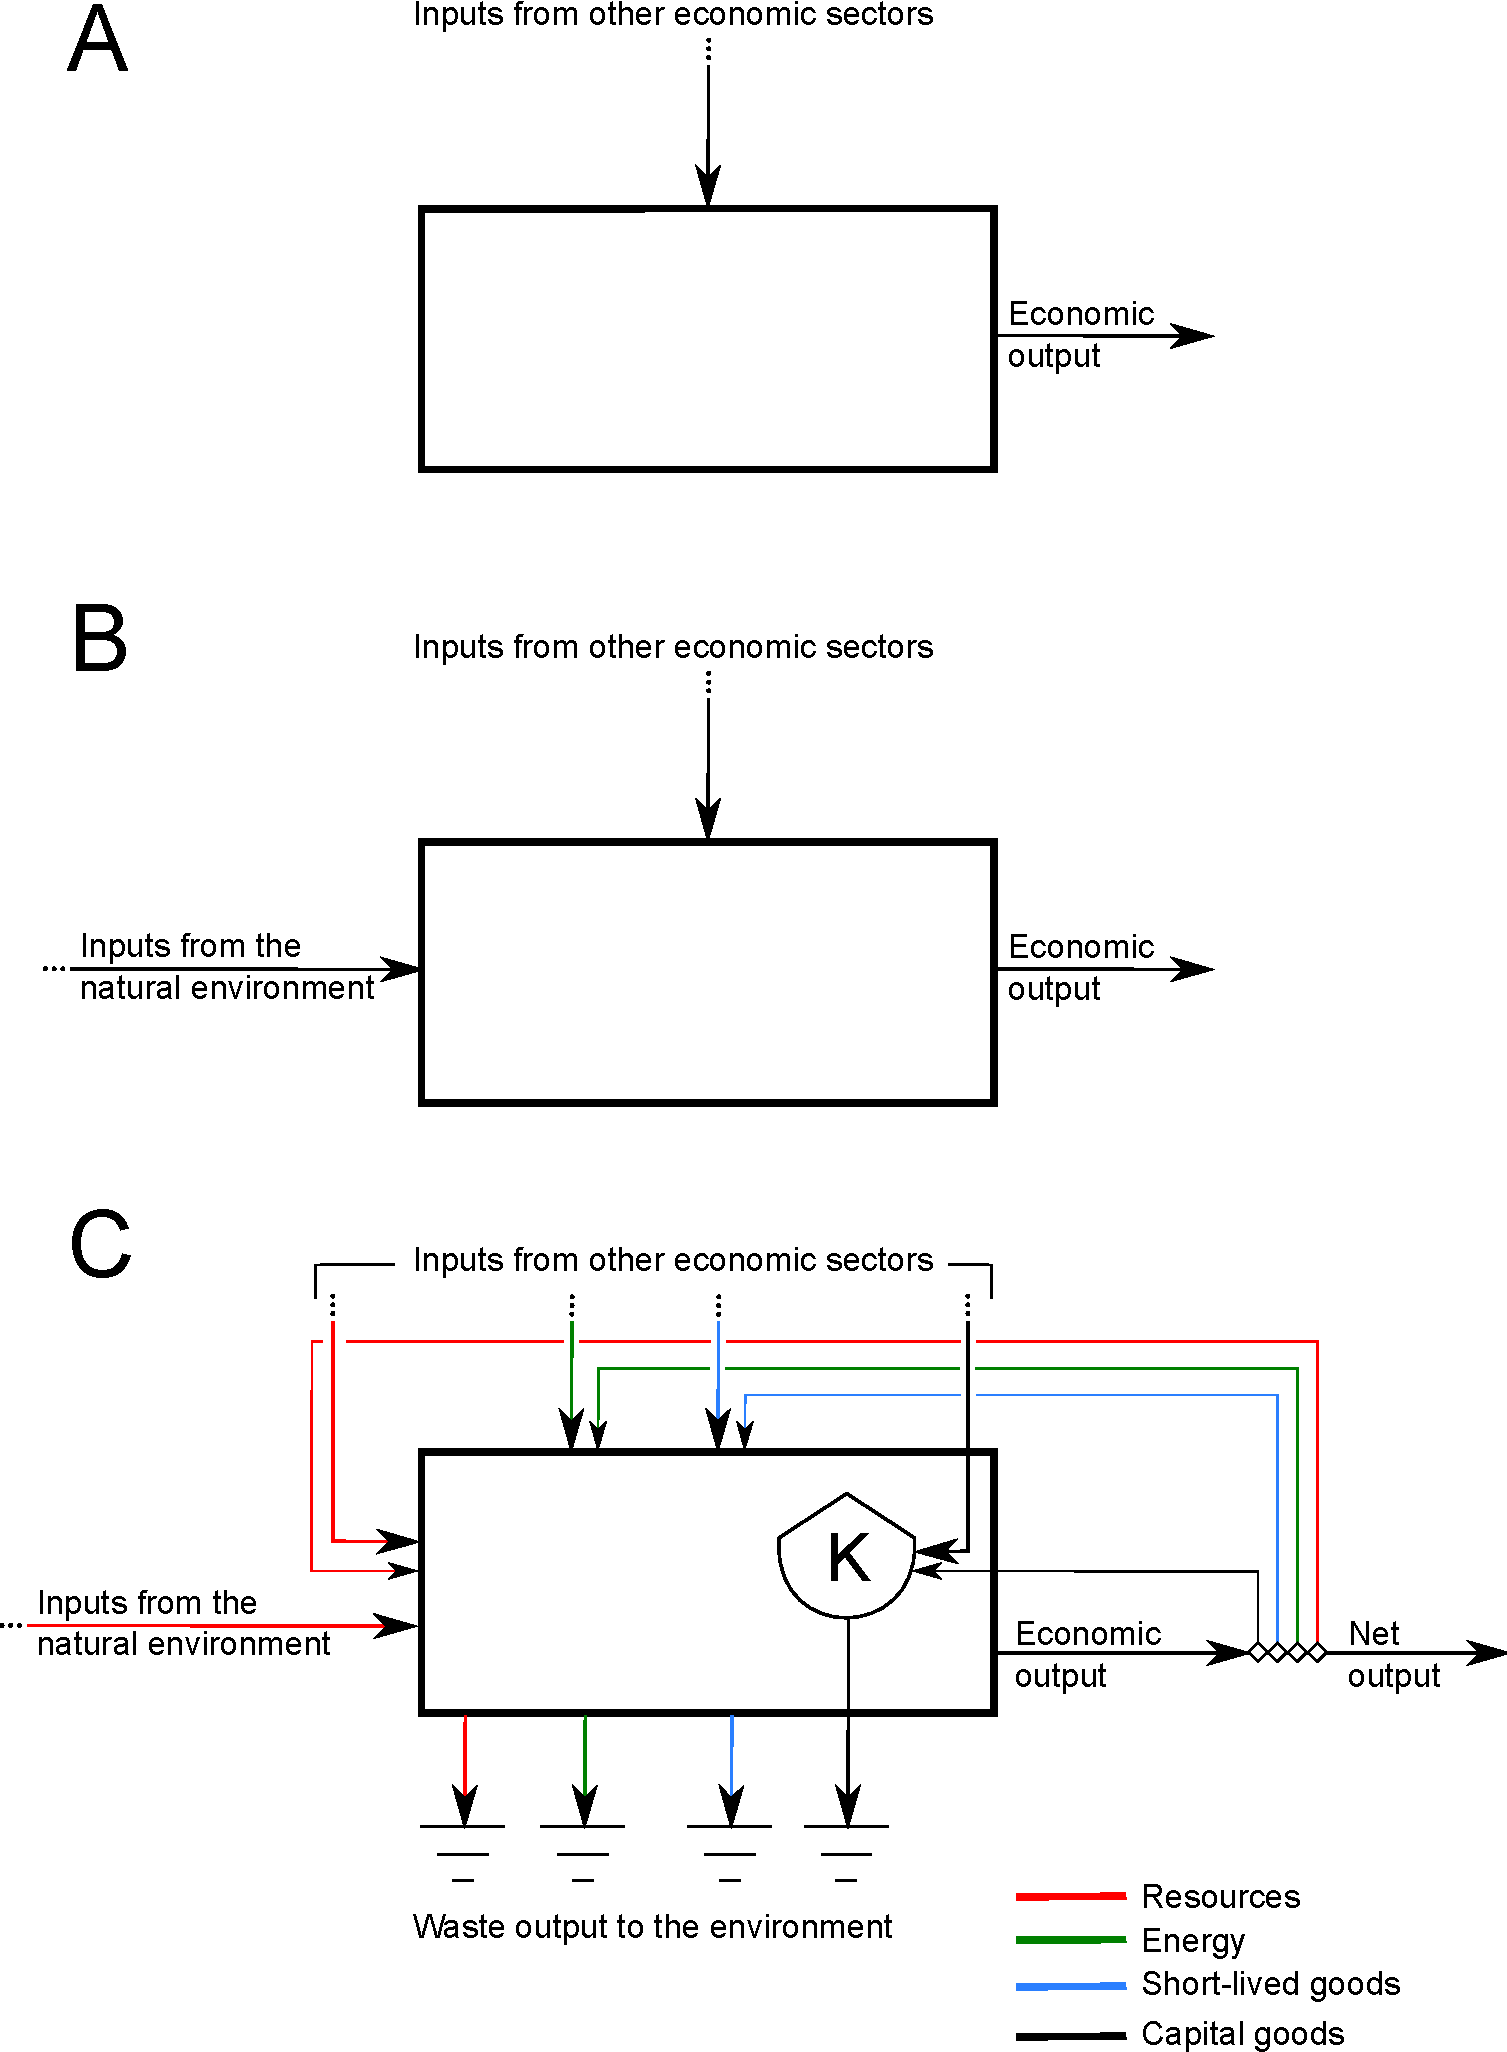
\includegraphics[width=0.8\linewidth]{Chapter_Methodology/images/Basic_unit_v5.pdf}
\caption{The basic unit of input-output modeling: A) the standard economic approach includes only transactions among sectors of the economy; B) the ecological economics approach models inputs from the natural environment outside the economy as factors of production and; C) the method presented here accounts also for accumulation, K, of embodied energy within materials in economic sectors.}
\label{fig:basic_unit}
\end{figure}

%%%%%%%%%% Methodology %%%%%%%%%%
\section{Total energy ($T$)}
%%%%%%%%%%

Total energy ($T$) is the sum of the direct and indirect (embodied) energy.

\begin{equation} \label{eq:T_def}
	T \equiv E + B
\end{equation}

In general, the flow rate of total energy among sectors in the economy, the earth, and society is given by

\begin{equation} \label{eq:T_dot_def}
	\dot{T} = \dot{E} + \dot{B}.
\end{equation}

In some cases, total energy flows may consist of direct energy ($\dot{E}$) or embodied energy ($\dot{B}$) exclusively. For example, the flow of extracted crude oil from the earth consists of direct energy only ($\dot{B} = 0$ and $\dot{T} = \dot{E}$), because, in this method, no embodied energy ($B$) has been added to the crude oil until it reaches the downstream side of the pump. The flow of goods produced by a non-energy sector of the economy consists of indirect energy only ($\dot{E} = 0$, and therefore $\dot{T} = \dot{B}$), because no direct energy ($E$) is produced by a non-energy sector in this model economy. 

In other cases, total energy flows may have both direct \emph{and} indirect components. For example, the flow of refined petroleum from the energy sector has both a direct energy ($\dot{E}$, the energy content of the oil product, usually represented by chemical potential energy) and embodied energy ($\dot{B}$, which accounts for the energy consumed in upstream processes to extract and refine the crude oil).\footnote{Outputs from agricultural sectors will be similar: both the direct energy component (comprising chemical potential energy) and the embodied energy component will be non-zero.}

Single subscripts on $T$, $E$, or $B$ can mean one of two things: $\dot{T}_{i}$ indicates the outflow of total energy from sector $i$, whereas $T_{i}$ denotes the total energy content of sector $i$. Double subscripts on $T$, $E$, or $B$ (e.g., $\dot{T}_{ij}$) indicate a flow from sector $i$ to sector $j$,\footnote{In the following discussion, the first index always indicates the sector \emph{from} which a quantity flows, and the second index indicates the sector \emph{to} which a quantity flows.} in this case for total energy ($T$).  

The I-O literature \cite{Bullard1975, Herendeen1978} [REF TO BULLARD AND HERENDEEN, ETC. HERE --MKH] assumes (a) that steady state conditions exist (i.e., no accumulation of total energy in economic sectors) and (b) that flows of total energy ($\dot{T}$) are \emph{conserved}, where by \emph{conserved}, it is meant that total energy can be neither created nor destroyed. Like the literature, we assume that total energy is conserved. However, we depart from the literature to allow durability of goods as represented by total energy accumulation in economic sectors. Steady state, this approach is not.

Total energy may accumulate within an economic sector as stocks of direct energy materials (piles of coal or tanks of oil) but also as embodied energy in stocks of capital goods (e.g. machinery or buildings). The rate of accumulation of total energy ($\frac{dT}{dt}$) in a sector of the economy, the Earth, or society is given by the time derivative of total energy:

\begin{equation} \label{eq:T_accum_def}
	\frac{\mathrm{d}T}{\mathrm{d}t} = \frac{\mathrm{d}E}{\mathrm{d}t} + \frac{\mathrm{d}B}{\mathrm{d}t}.
\end{equation}

We note that the definition of total energy (Equation \ref{eq:T_def}) includes direct energy ($E$) and embodied energy ($B$) terms. On the other hand, the First Law of Thermodynamics includes direct energy ($E$) and waste heat ($Q$) terms. The consequence of the foregoing difference is that an interesting relationship exists between embodied energy ($B$) and waste heat ($Q$). We shall see in the following example that waste heat from an economic sector can be considered to contribute to energy embodied within the products of that sector.


\bibliography{EROI_review_v2}
\bibliographystyle{unsrt}


% Always give a unique label
% and use \ref{<label>} for cross-references
% and \cite{<label>} for bibliographic references
% use \sectionmark{}
% to alter or adjust the section heading in the running head
%% Instead of simply listing headings of different levels we recommend to let every heading be followed by at least a short passage of text. Furtheron please use the \LaTeX\ automatism for all your cross-references and citations.

%% Please note that the first line of text that follows a heading is not indented, whereas the first lines of all subsequent paragraphs are.

%% Use the standard \verb|equation| environment to typeset your equations, e.g.
%
%% \begin{equation}
%% a \times b = c\;,
%% \end{equation}
%
%% however, for multiline equations we recommend to use the \verb|eqnarray|
%% environment\footnote{In physics texts please activate the class option \texttt{vecphys} to depict your vectors in \textbf{\itshape boldface-italic} type - as is customary for a wide range of physical subjects.}.
%% \begin{eqnarray}
%% a \times b = c \nonumber\\
%% \vec{a} \cdot \vec{b}=\vec{c}
%% \label{eq:01}
%% \end{eqnarray}

%% \subsection{Subsection Heading}
%% \label{subsec:2}
%% Instead of simply listing headings of different levels we recommend to let every heading be followed by at least a short passage of text. Furtheron please use the \LaTeX\ automatism for all your cross-references\index{cross-references} and citations\index{citations} as has already been described in Sect.~\ref{sec:2}.

%% \begin{quotation}
%% Please do not use quotation marks when quoting texts! Simply use the \verb|quotation| environment -- it will automatically render Springer's preferred layout.
%% \end{quotation}


%% \subsubsection{Subsubsection Heading}
%% Instead of simply listing headings of different levels we recommend to let every heading be followed by at least a short passage of text. Furtheron please use the \LaTeX\ automatism for all your cross-references and citations as has already been described in Sect.~\ref{subsec:2}, see also Fig.~\ref{fig:1}\footnote{If you copy text passages, figures, or tables from other works, you must obtain \textit{permission} from the copyright holder (usually the original publisher). Please enclose the signed permission with the manucript. The sources\index{permission to print} must be acknowledged either in the captions, as footnotes or in a separate section of the book.}

%% Please note that the first line of text that follows a heading is not indented, whereas the first lines of all subsequent paragraphs are.

% For figures use
%
%% \begin{figure}[b]
%% \sidecaption
% Use the relevant command for your figure-insertion program
% to insert the figure file.
% For example, with the option graphics use
%% \includegraphics[scale=.65]{figure}
%
% If not, use
%\picplace{5cm}{2cm} % Give the correct figure height and width in cm
%
%% \caption{If the width of the figure is less than 7.8 cm use the \texttt{sidecapion} command to flush the caption on the left side of the page. If the figure is positioned at the top of the page, align the sidecaption with the top of the figure -- to achieve this you simply need to use the optional argument \texttt{[t]} with the \texttt{sidecaption} command}
%% \label{fig:1}       % Give a unique label
%% \end{figure}


%% \paragraph{Paragraph Heading} %
%% Instead of simply listing headings of different levels we recommend to let every heading be followed by at least a short passage of text. Furtheron please use the \LaTeX\ automatism for all your cross-references and citations as has already been described in Sect.~\ref{sec:2}.

%% Please note that the first line of text that follows a heading is not indented, whereas the first lines of all subsequent paragraphs are.

%% For typesetting numbered lists we recommend to use the \verb|enumerate| environment -- it will automatically render Springer's preferred layout.

%% \begin{enumerate}
%% \item{Livelihood and survival mobility are oftentimes coutcomes of uneven socioeconomic development.}
%% \begin{enumerate}
%% \item{Livelihood and survival mobility are oftentimes coutcomes of uneven socioeconomic development.}
%% \item{Livelihood and survival mobility are oftentimes coutcomes of uneven socioeconomic development.}
%% \end{enumerate}
%% \item{Livelihood and survival mobility are oftentimes coutcomes of uneven socioeconomic development.}
%% \end{enumerate}


%% \subparagraph{Subparagraph Heading} In order to avoid simply listing headings of different levels we recommend to let every heading be followed by at least a short passage of text. Use the \LaTeX\ automatism for all your cross-references and citations as has already been described in Sect.~\ref{sec:2}, see also Fig.~\ref{fig:2}.

%% Please note that the first line of text that follows a heading is not indented, whereas the first lines of all subsequent paragraphs are.

%% For unnumbered list we recommend to use the \verb|itemize| environment -- it will automatically render Springer's preferred layout.

%% \begin{itemize}
%% \item{Livelihood and survival mobility are oftentimes coutcomes of uneven socioeconomic development, cf. Table~\ref{tab:1}.}
%% \begin{itemize}
%% \item{Livelihood and survival mobility are oftentimes coutcomes of uneven socioeconomic development.}
%% \item{Livelihood and survival mobility are oftentimes coutcomes of uneven socioeconomic development.}
%% \end{itemize}
%% \item{Livelihood and survival mobility are oftentimes coutcomes of uneven socioeconomic development.}
%% \end{itemize}

%% \begin{figure}[t]
%% \sidecaption[t]
% Use the relevant command for your figure-insertion program
% to insert the figure file.
% For example, with the option graphics use
%% \includegraphics[scale=.65]{figure}
%
% If not, use
%\picplace{5cm}{2cm} % Give the correct figure height and width in cm
%
%% \caption{Please write your figure caption here}
%% \label{fig:2}       % Give a unique label
%% \end{figure}

%% \runinhead{Run-in Heading Boldface Version} Use the \LaTeX\ automatism for all your cross-references and citations as has already been described in Sect.~\ref{sec:2}.

%% \subruninhead{Run-in Heading Italic Version} Use the \LaTeX\ automatism for all your cross-refer\-ences and citations as has already been described in Sect.~\ref{sec:2}\index{paragraph}.
% Use the \index{} command to code your index words
%
% For tables use
%
%% \begin{table}
%% \caption{Please write your table caption here}
%% \label{tab:1}       % Give a unique label
%
% For LaTeX tables use
%
%% \begin{tabular}{p{2cm}p{2.4cm}p{2cm}p{4.9cm}}
%% \hline\noalign{\smallskip}
%% Classes & Subclass & Length & Action Mechanism  \\
%% \noalign{\smallskip}\svhline\noalign{\smallskip}
%% Translation & mRNA$^a$  & 22 (19--25) & Translation repression, mRNA cleavage\\
%% Translation & mRNA cleavage & 21 & mRNA cleavage\\
%% Translation & mRNA  & 21--22 & mRNA cleavage\\
%%Translation & mRNA  & 24--26 & Histone and DNA Modification\\
%%\noalign{\smallskip}\hline\noalign{\smallskip}
%%\end{tabular}
%%$^a$ Table foot note (with superscript)
%%\end{table}
%
%% \section{Section Heading}
%%\label{sec:3}
% Always give a unique label
% and use \ref{<label>} for cross-references
% and \cite{<label>} for bibliographic references
% use \sectionmark{}
% to alter or adjust the section heading in the running head
%% Instead of simply listing headings of different levels we recommend to let every heading be followed by at least a short passage of text. Furtheron please use the \LaTeX\ automatism for all your cross-references and citations as has already been described in Sect.~\ref{sec:2}.

%% Please note that the first line of text that follows a heading is not indented, whereas the first lines of all subsequent paragraphs are.

%%If you want to list definitions or the like we recommend to use the Springer-enhanced \verb|description| environment -- it will automatically render Springer's preferred layout.

%%\begin{description}[Type 1]
%%\item[Type 1]{That addresses central themes pertainng to migration, health, and disease. In Sect.~\ref{sec:1}, Wilson discusses the role of human migration in infectious disease distributions and patterns.}
%%\item[Type 2]{That addresses central themes pertainng to migration, health, and disease. In Sect.~\ref{subsec:2}, Wilson discusses the role of human migration in infectious disease distributions and patterns.}
%%\end{description}

%%\subsection{Subsection Heading} %
%% In order to avoid simply listing headings of different levels we recommend to let every heading be followed by at least a short passage of text. Use the \LaTeX\ automatism for all your cross-references and citations citations as has already been described in Sect.~\ref{sec:2}.

%% Please note that the first line of text that follows a heading is not indented, whereas the first lines of all subsequent paragraphs are.

%% \begin{svgraybox}
%% If you want to emphasize complete paragraphs of texts we recommend to use the newly defined Springer class option \verb|graybox| and the newly defined environment \verb|svgraybox|. This will produce a 15 percent screened box 'behind' your text.

%% If you want to emphasize complete paragraphs of texts we recommend to use the newly defined Springer class option and environment \verb|svgraybox|. This will produce a 15 percent screened box 'behind' your text.
%% \end{svgraybox}


%% \subsubsection{Subsubsection Heading}
%%Instead of simply listing headings of different levels we recommend to let every heading be followed by at least a short passage of text. Furtheron please use the \LaTeX\ automatism for all your cross-references and citations as has already been described in Sect.~\ref{sec:2}.

%% Please note that the first line of text that follows a heading is not indented, whereas the first lines of all subsequent paragraphs are.

%% \begin{theorem}
%% Theorem text goes here.
%% \end{theorem}
%
% or
%
%% \begin{definition}
%% Definition text goes here.
%% \end{definition}

%% \begin{proof}
%\smartqed
%% Proof text goes here.
%% \qed
%% \end{proof}

%%\paragraph{Paragraph Heading} %
%% Instead of simply listing headings of different levels we recommend to let every heading be followed by at least a short passage of text. Furtheron please use the \LaTeX\ automatism for all your cross-references and citations as has already been described in Sect.~\ref{sec:2}.

%% Note that the first line of text that follows a heading is not indented, whereas the first lines of all subsequent paragraphs are.
%
% For built-in environments use
%
%%\begin{theorem}
%%Theorem text goes here.
%%\end{theorem}
%
%%\begin{definition}
%%Definition text goes here.
%%\end{definition}
%
%%\begin{proof}
%%\smartqed
%% Proof text goes here.
%%\qed
%%\end{proof}
%
%% \begin{acknowledgement}
%% If you want to include acknowledgments of assistance and the like at the end of an individual chapter please use the \verb|acknowledgement| environment -- it will automatically render Springer's preferred layout.
%% \end{acknowledgement}
%
%% \section*{Appendix}
%% \addcontentsline{toc}{section}{Appendix}
%
%% When placed at the end of a chapter or contribution (as opposed to at the end of the book), the numbering of tables, figures, and equations in the appendix section continues on from that in the main text. Hence please \textit{do not} use the \verb|appendix| command when writing an appendix at the end of your chapter or contribution. If there is only one the appendix is designated ``Appendix'', or ``Appendix 1'', or ``Appendix 2'', etc. if there is more than one.

%% \begin{equation}
%% a \times b = c
%% \end{equation}
% Problems or Exercises should be sorted chapterwise
%% \section*{Problems}
%% \addcontentsline{toc}{section}{Problems}
%
% Use the following environment.
% Don't forget to label each problem;
% the label is needed for the solutions' environment
%% \begin{prob}
%% \label{prob1}
%% A given problem or Excercise is described here. The
%% problem is described here. The problem is described here.
%% \end{prob}

%% \begin{prob}
%% \label{prob2}
%% \textbf{Problem Heading}\\
%% (a) The first part of the problem is described here.\\
%% (b) The second part of the problem is described here.
%% \end{prob}




%%%%%%%%%%%%%%%%%%%%% chapter.tex %%%%%%%%%%%%%%%%%%%%%%%%%%%%%%%%%
%
% sample chapter
%
% Use this file as a template for your own input.
%
%%%%%%%%%%%%%%%%%%%%%%%% Springer-Verlag %%%%%%%%%%%%%%%%%%%%%%%%%%
%\motto{Use the template \emph{chapter.tex} to style the various elements of your chapter content.}
\chapter{Example A: single sector economy}
\chaptermark{Example A}
\label{chap:single_sector} % Always give a unique label
% use \chaptermark{}
% to alter or adjust the chapter heading in the running head

\abstract*{[NEED TO ADD ABSTRACT HERE]}

%% \abstract{Each chapter should be preceded by an abstract (10--15 lines long) that summarizes the content. The abstract will appear \textit{online} at \url{www.SpringerLink.com} and be available with unrestricted access. This allows unregistered users to read the abstract as a teaser for the complete chapter. As a general rule the abstracts will not appear in the printed version of your book unless it is the style of your particular book or that of the series to which your book belongs.\newline\indent
%% Please use the 'starred' version of the new Springer \texttt{abstract} command for typesetting the text of the online abstracts (cf. source file of this chapter template \texttt{abstract}) and include them with the source files of your manuscript. Use the plain \texttt{abstract} command if the abstract is also to appear in the printed version of the book.}

%% Use the template \emph{chapter.tex} together with the Springer document class SVMono (monograph-type books) or SVMult (edited books) to style the various elements of your chapter content in the Springer layout.

In this section, we present an example economic analysis using a single-sector economy wherein the economy and society are merged together.

Figure \ref{fig:single_sector_flows_0} shows a single-sector Economy (represented by ``economy/society,'' 2) that extracts direct energy from the earth ($\dot{E}_{12}$). Direct energy and waste heat flows are identified by vectors. No direct energy flows from the economy (2) to the earth (1), only waste heat ($\dot{Q}_{21}$).

\begin{figure}[h!]
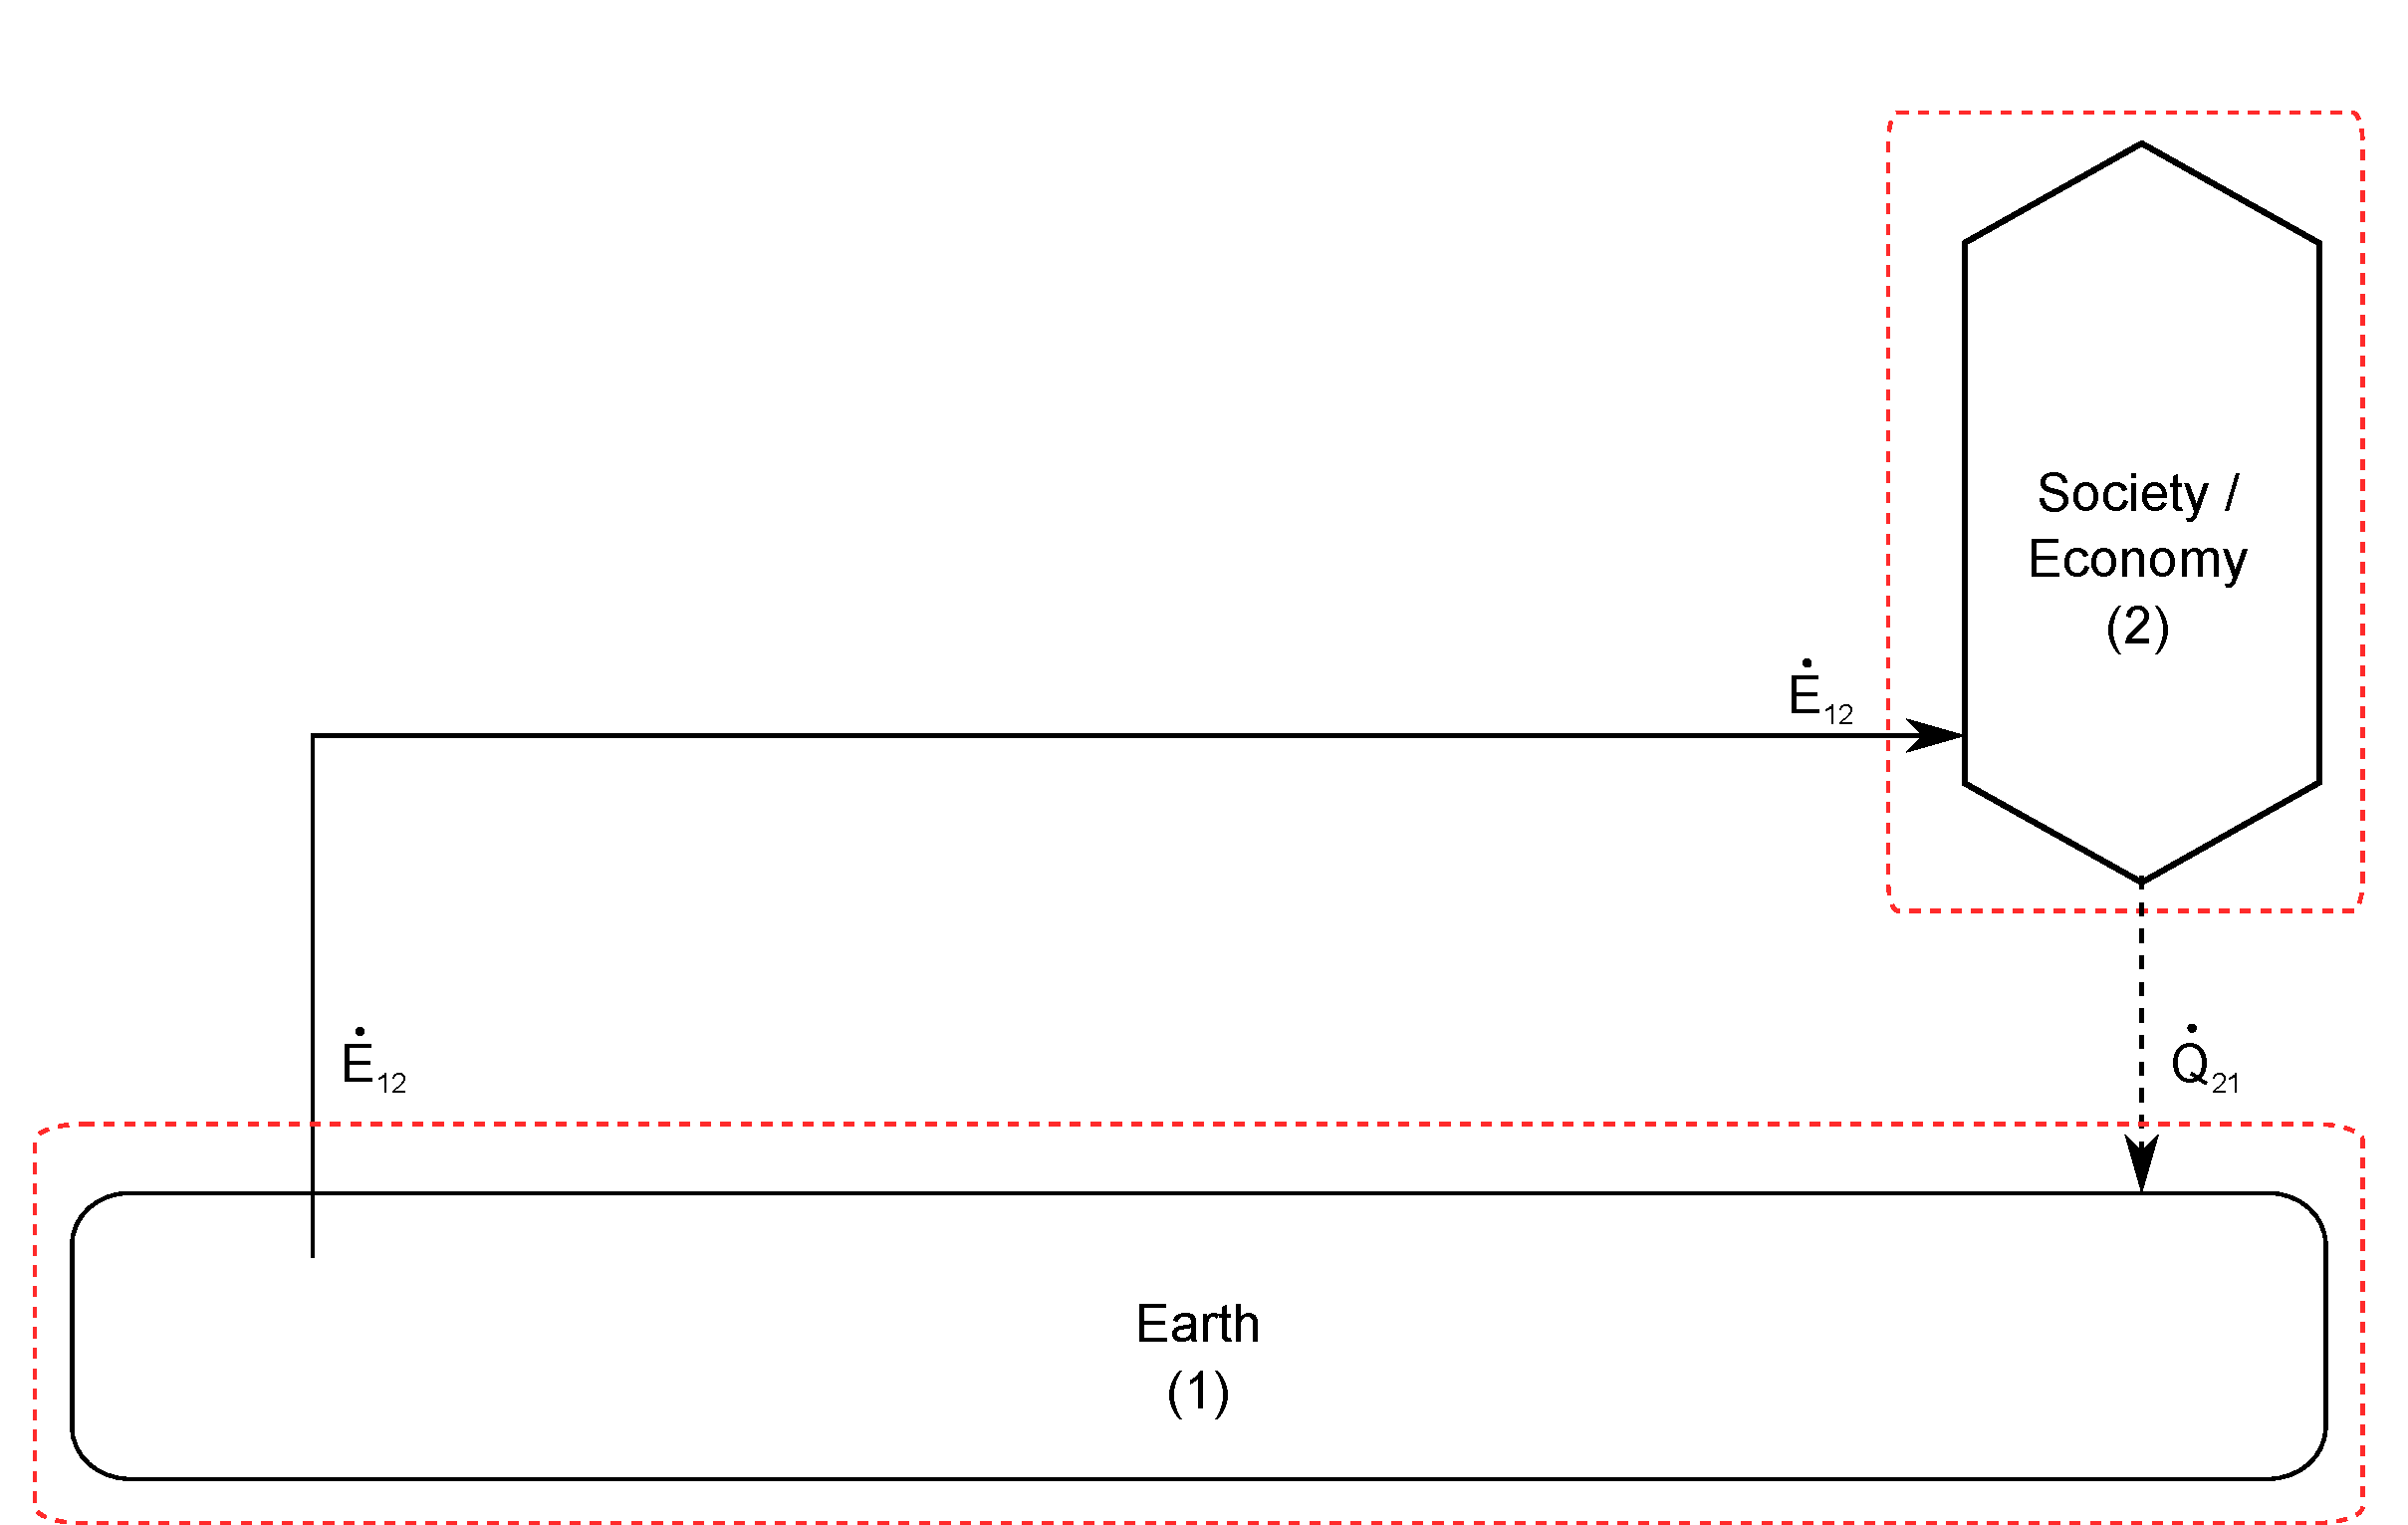
\includegraphics[width=1.0\linewidth]{Chapter_Example_A/images/I-O_one_sector_direct_energy.pdf}
\caption{Direct energy ($\dot{E}$) and waste heat ($\dot{Q}$) flows for a single-sector economy. }
\label{fig:single_sector_flows_0}
\end{figure}

%%%%%%%%%% Example A %%%%%%%%%%
\section{First Law of Thermodynamics}
%%%%%%%%%%

Both direct energy ($\dot{E}$, such as the energy content of coal, oil, and electricity), and waste heat ($\dot{Q}$) are accounted by the First Law of Thermodynamics. Accounting for possible accumulation of direct energy in the economy, the First Law of Thermodynamics indicates that

\begin{equation} \label{eq:dE_2/dt_single_sector}
	\frac{\mathrm{d}E_{2}}{\mathrm{d}t} = \dot{E}_{12} - \dot{Q}_{21}.
\end{equation}

Aside from, for example, the U.S. Strategic Petroleum Reserve, we are not stockpiling oil and coal at any meaningful rate, i.e. we consume fossil fuels at a rate equal to the extraction rate. Thus, the world is not accumulating direct energy in the economy.\footnote{A counter-example could be made for nuclear fuels where `spent' fuel represents a large exergetic stockpile, however, this reserve is not (presently) economically useful.} (The world \emph{is}, however, accumulating embodied energy in the economy as we shall see shortly.) Thus, the accumulation rate for direct energy $\left(\frac{\mathrm{d}E_{2}}{\mathrm{d}t}\right)$ in the above equation can be set to zero to obtain

\begin{equation} \label{eq:single_sector_direct_energy_no_accumulation}
	0 = \dot{E}_{12} - \dot{Q}_{21}.
\end{equation}

%%%%%%%%%% Example A %%%%%%%%%%
\section{Total energy accounting}
%%%%%%%%%%

Figure \ref{fig:single_sector_flows_2} shows the flows of total energy ($\dot{T}$) through the single-sector economy.

\begin{figure}[h!]
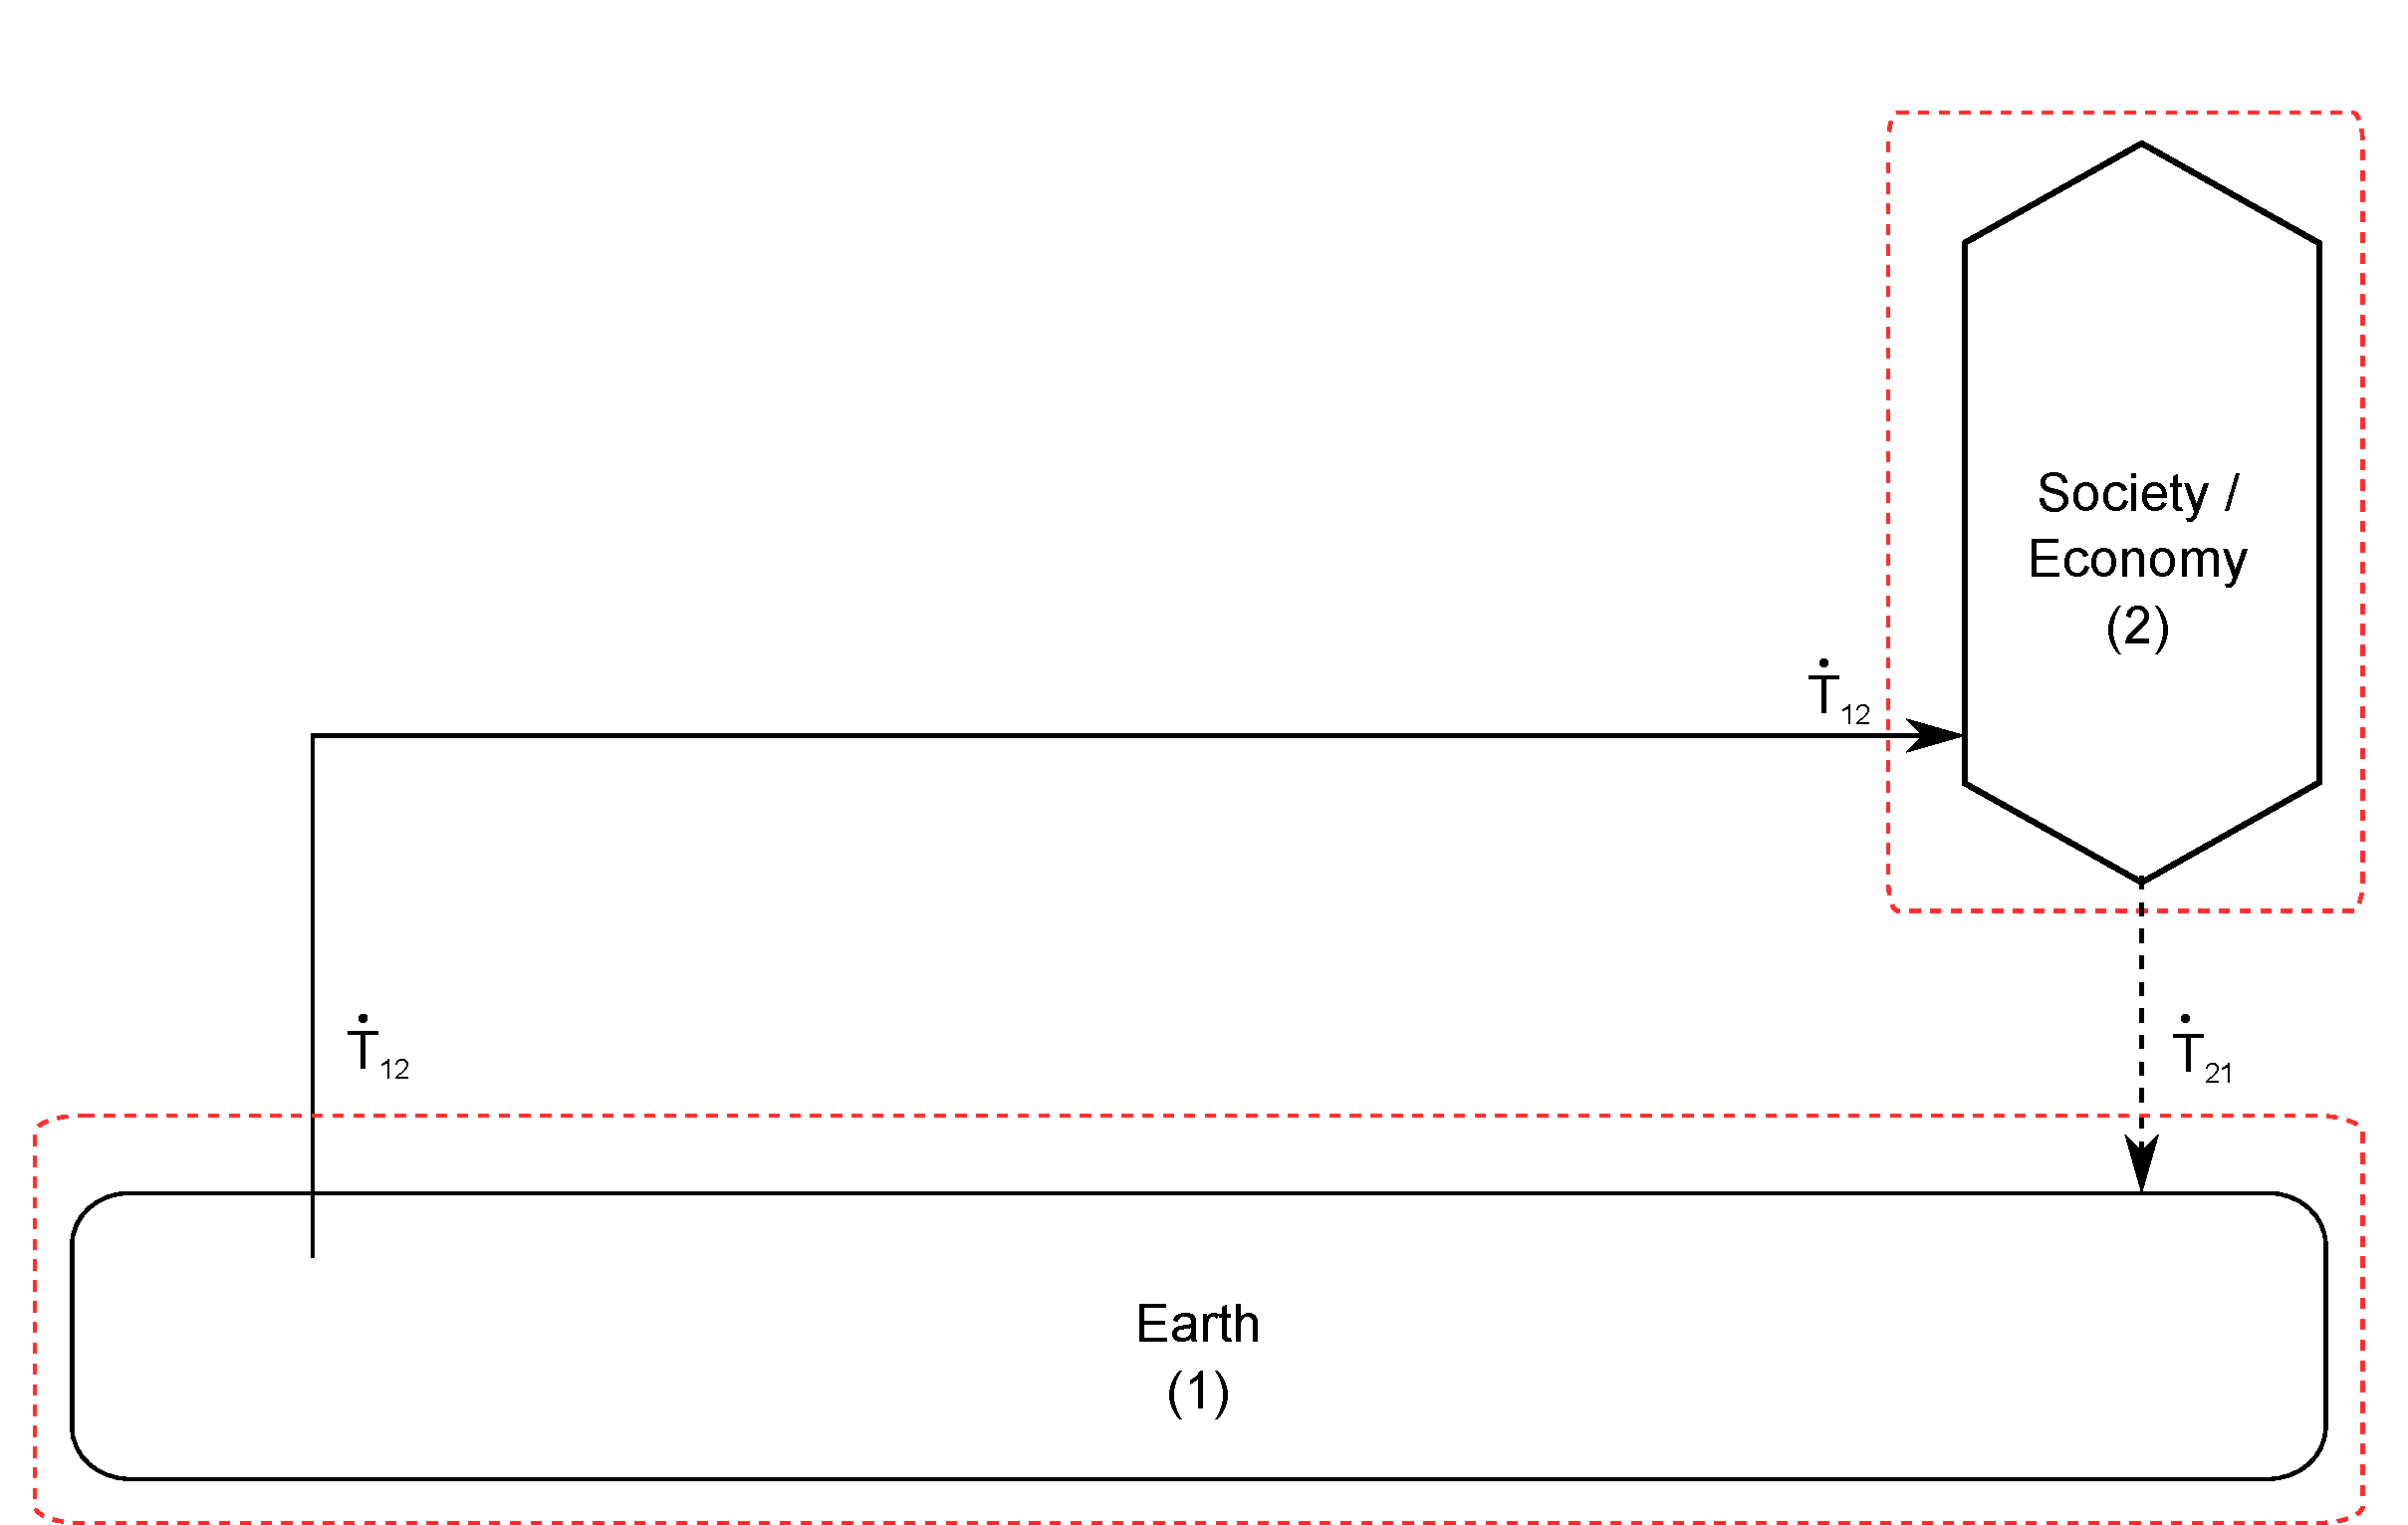
\includegraphics[width=1.0\linewidth]{Chapter_Example_A/images/I-O_one_sector_total_energy.pdf}
\caption{Total Energy Flows ($\dot{T}$) in a Single-sector Economy.}
\label{fig:single_sector_flows_2}
\end{figure}

We follow the I-O literature in assuming that total energy ($T$) is conserved. The I-O literature assumes steady-state operation of the economy with no accumulation of embodied energy in the economic sectors. (We will see later how the assumption in the literature introduces errors into I-O analyses.) We depart from the I-O literature by accounting for both accumulation and depreciation of energy embodied in sectors of the economy and society. By doing so, the present analysis does \emph{not} assume a steady-state economy. A total energy accounting around the single-sector economy (2) gives

\begin{equation} \label{eq:single_sector_T_with_accumulation}
	\frac{\mathrm{d}T_{2}}{\mathrm{d}t} = \dot{T}_{12}  - \dot{T}_{21}.
\end{equation}

%%%%%%%%%% Example A %%%%%%%%%%
\section{Embodied energy accounting}
%%%%%%%%%%

The First Law of Thermodynamics accounts for both direct energy ($E$) and waste heat ($Q$), whereas total energy ($T$) accounting tracks direct energy ($E$) and embodied energy ($B$). If we substitute the First Law into the total energy accounting equation, we can eliminate direct energy ($E$) to arrive at an embodied energy accounting equation. We begin by expanding the $T$ terms in Equation \ref{eq:single_sector_T_with_accumulation} using Equations \ref{eq:T_def} and \ref{eq:T_dot_def} to obtain

\begin{equation} \label{eq:single_sector_T_with_accumulation_expanded_T}
	\frac{\mathrm{d}E_{2}}{\mathrm{d}t} + \frac{\mathrm{d}B_{2}}{\mathrm{d}t} = \dot{E}_{12} + \dot{B}_{12} - \dot{E}_{21} - \dot{B}_{21}.
\end{equation}

\noindent Realizing that $\frac{\mathrm{d}E_2}{\mathrm{d}t} = 0$ (because direct energy does not accumulate in meaningful amounts in the economy) and $\dot{E}_{21} = 0$ (because energy is returned to the earth as waste heat, see Figure \ref{fig:single_sector_flows_0}) yields

\begin{equation} \label{eq:single_sector_B_accumulation}
	\frac{\mathrm{d}B_{2}}{\mathrm{d}t} = \dot{E}_{12} + \dot{B}_{12} - \dot{B}_{21}.
\end{equation}

\noindent Equation \ref{eq:single_sector_B_accumulation} shows that the accumulation rate of embodied energy in the economy is a function of the inflows of direct and embodied energy less the outflow of embodied energy. 

In this example, we substitute\footnote{We shall encounter this move to substitute the First Law of Thermodynamics into the total energy accounting equation repeatedly below.} Equation \ref{eq:single_sector_direct_energy_no_accumulation} into Equation \ref{eq:single_sector_B_accumulation} to obtain an embodied energy accounting equation:

\begin{equation} \label{eq:embodied_energy_accounting}
	\frac{\mathrm{d}B_{2}}{\mathrm{d}t} = \dot{Q}_{21} + \dot{B}_{12} - \dot{B}_{21}.
\end{equation}

An important result of Bullard-Herendeen-style I-O analyses, historically, has been the quantification of the embodied energy content of economic sector outputs, in this case $\dot{B}_{21}$. Equation \ref{eq:single_sector_B_accumulation} can be rearranged to give

\begin{equation} \label{eq:single_sector_B_output}
	\dot{B}_{21} = \dot{Q}_{21} + \dot{B}_{12} - \frac{\mathrm{d}B_{2}}{\mathrm{d}t}.
\end{equation}

Equation \ref{eq:single_sector_B_output} indicates that the embodied energy content of the product of an economic sector (in this case $\dot{B}_{21}$) can be thought of as the sum of the embodied energy inputs to the sector (in this case $\dot{B}_{12}$) and the waste heat from the sector (in this case $\dot{Q}_{21}$) less the accumulation rate of embodied energy in the sector (in this case $\frac{\mathrm{d}B_{2}}{\mathrm{d}t}$). This derivation indicates that waste heat ($\dot{Q}$) plays an important role\footnote{To our knowledge, there has been no prior identification of the role of waste heat in Bullard-Herendeen-style I-O analyses.} in Bullard-Herendeen-style I-O analyses: the accumulation of waste heat along a production path leads to energy being `embodied' in the output of an economic sector. 

In Equation \ref{eq:single_sector_B_output} we also see the first indication that the traditional approach of neglecting dynamic effects in I-O analyses may lead to errors. If $\frac{\mathrm{d}B_2}{\mathrm{d}t}$ is both neglected and nonzero, calculation of the embodied energy outflow rate ($\dot{B}_{21}$) will be in error.

%%%%%%%%%% Example A %%%%%%%%%%
\section{Depreciation}
%%%%%%%%%%

It is worthwhile to note that $\dot{B}_{21}$ represents the disposal rate of embodied energy from the economy back to the earth, akin to depreciation of physical assets. This physical depreciation is different from, but related to, financial depreciation, as financial depreciation is usually faster than physical depreciation. Embodied energy depreciation ($\dot{B}_{21}$ in this example) can be represented by a depreciation term such as

\begin{equation} \label{eq:depreciation_term_defined}
	\dot{B}_{21} = \gamma_{2}B_{2},
\end{equation}

\noindent where $\gamma$ represents the depreciation rate in units of inverse time (e.g., 1/year) with $\gamma > 0$. The depreciation rate ($\gamma$) indicates that a fraction of the total stock of embodied energy is disposed over a period of time (e.g, $\gamma = 0.05$/year). In the absence of other inputs or outputs, this depreciation function provides exponential decay of embodied energy ($B$). $\gamma$ is, in general, a function of time.

Equation \ref{eq:depreciation_term_defined} can be substituted into Equation \ref{eq:embodied_energy_accounting} and rearranged to obtain 

\begin{equation} \label{eq:dB2/dt_single_sector_with_depreciation_gamma}
	\frac{\mathrm{d}B_{2}}{\mathrm{d}t} =  \dot{Q}_{21} + \dot{B}_{12} - \gamma_{2}B_{2}
\end{equation}

\noindent which indicates that the accumulation rate of embodied energy in an economic sector (in this case $\frac{\mathrm{d}B_{2}}{\mathrm{d}t}$) is equal to the sum of the waste heat rate from the economic sector ($\dot{Q}_{21}$) and the inflow rate of embodied energy to the sector ($\dot{B}_{12}$) less the embodied energy disposal rate ($\gamma_{2}B_{2}$).


\bibliography{EROI_review_v2}
\bibliographystyle{unsrt}


% Always give a unique label
% and use \ref{<label>} for cross-references
% and \cite{<label>} for bibliographic references
% use \sectionmark{}
% to alter or adjust the section heading in the running head
%% Instead of simply listing headings of different levels we recommend to let every heading be followed by at least a short passage of text. Furtheron please use the \LaTeX\ automatism for all your cross-references and citations.

%% Please note that the first line of text that follows a heading is not indented, whereas the first lines of all subsequent paragraphs are.

%% Use the standard \verb|equation| environment to typeset your equations, e.g.
%
%% \begin{equation}
%% a \times b = c\;,
%% \end{equation}
%
%% however, for multiline equations we recommend to use the \verb|eqnarray|
%% environment\footnote{In physics texts please activate the class option \texttt{vecphys} to depict your vectors in \textbf{\itshape boldface-italic} type - as is customary for a wide range of physical subjects.}.
%% \begin{eqnarray}
%% a \times b = c \nonumber\\
%% \vec{a} \cdot \vec{b}=\vec{c}
%% \label{eq:01}
%% \end{eqnarray}

%% \subsection{Subsection Heading}
%% \label{subsec:2}
%% Instead of simply listing headings of different levels we recommend to let every heading be followed by at least a short passage of text. Furtheron please use the \LaTeX\ automatism for all your cross-references\index{cross-references} and citations\index{citations} as has already been described in Sect.~\ref{sec:2}.

%% \begin{quotation}
%% Please do not use quotation marks when quoting texts! Simply use the \verb|quotation| environment -- it will automatically render Springer's preferred layout.
%% \end{quotation}


%% \subsubsection{Subsubsection Heading}
%% Instead of simply listing headings of different levels we recommend to let every heading be followed by at least a short passage of text. Furtheron please use the \LaTeX\ automatism for all your cross-references and citations as has already been described in Sect.~\ref{subsec:2}, see also Fig.~\ref{fig:1}\footnote{If you copy text passages, figures, or tables from other works, you must obtain \textit{permission} from the copyright holder (usually the original publisher). Please enclose the signed permission with the manucript. The sources\index{permission to print} must be acknowledged either in the captions, as footnotes or in a separate section of the book.}

%% Please note that the first line of text that follows a heading is not indented, whereas the first lines of all subsequent paragraphs are.

% For figures use
%
%% \begin{figure}[b]
%% \sidecaption
% Use the relevant command for your figure-insertion program
% to insert the figure file.
% For example, with the option graphics use
%% \includegraphics[scale=.65]{figure}
%
% If not, use
%\picplace{5cm}{2cm} % Give the correct figure height and width in cm
%
%% \caption{If the width of the figure is less than 7.8 cm use the \texttt{sidecapion} command to flush the caption on the left side of the page. If the figure is positioned at the top of the page, align the sidecaption with the top of the figure -- to achieve this you simply need to use the optional argument \texttt{[t]} with the \texttt{sidecaption} command}
%% \label{fig:1}       % Give a unique label
%% \end{figure}


%% \paragraph{Paragraph Heading} %
%% Instead of simply listing headings of different levels we recommend to let every heading be followed by at least a short passage of text. Furtheron please use the \LaTeX\ automatism for all your cross-references and citations as has already been described in Sect.~\ref{sec:2}.

%% Please note that the first line of text that follows a heading is not indented, whereas the first lines of all subsequent paragraphs are.

%% For typesetting numbered lists we recommend to use the \verb|enumerate| environment -- it will automatically render Springer's preferred layout.

%% \begin{enumerate}
%% \item{Livelihood and survival mobility are oftentimes coutcomes of uneven socioeconomic development.}
%% \begin{enumerate}
%% \item{Livelihood and survival mobility are oftentimes coutcomes of uneven socioeconomic development.}
%% \item{Livelihood and survival mobility are oftentimes coutcomes of uneven socioeconomic development.}
%% \end{enumerate}
%% \item{Livelihood and survival mobility are oftentimes coutcomes of uneven socioeconomic development.}
%% \end{enumerate}


%% \subparagraph{Subparagraph Heading} In order to avoid simply listing headings of different levels we recommend to let every heading be followed by at least a short passage of text. Use the \LaTeX\ automatism for all your cross-references and citations as has already been described in Sect.~\ref{sec:2}, see also Fig.~\ref{fig:2}.

%% Please note that the first line of text that follows a heading is not indented, whereas the first lines of all subsequent paragraphs are.

%% For unnumbered list we recommend to use the \verb|itemize| environment -- it will automatically render Springer's preferred layout.

%% \begin{itemize}
%% \item{Livelihood and survival mobility are oftentimes coutcomes of uneven socioeconomic development, cf. Table~\ref{tab:1}.}
%% \begin{itemize}
%% \item{Livelihood and survival mobility are oftentimes coutcomes of uneven socioeconomic development.}
%% \item{Livelihood and survival mobility are oftentimes coutcomes of uneven socioeconomic development.}
%% \end{itemize}
%% \item{Livelihood and survival mobility are oftentimes coutcomes of uneven socioeconomic development.}
%% \end{itemize}

%% \begin{figure}[t]
%% \sidecaption[t]
% Use the relevant command for your figure-insertion program
% to insert the figure file.
% For example, with the option graphics use
%% \includegraphics[scale=.65]{figure}
%
% If not, use
%\picplace{5cm}{2cm} % Give the correct figure height and width in cm
%
%% \caption{Please write your figure caption here}
%% \label{fig:2}       % Give a unique label
%% \end{figure}

%% \runinhead{Run-in Heading Boldface Version} Use the \LaTeX\ automatism for all your cross-references and citations as has already been described in Sect.~\ref{sec:2}.

%% \subruninhead{Run-in Heading Italic Version} Use the \LaTeX\ automatism for all your cross-refer\-ences and citations as has already been described in Sect.~\ref{sec:2}\index{paragraph}.
% Use the \index{} command to code your index words
%
% For tables use
%
%% \begin{table}
%% \caption{Please write your table caption here}
%% \label{tab:1}       % Give a unique label
%
% For LaTeX tables use
%
%% \begin{tabular}{p{2cm}p{2.4cm}p{2cm}p{4.9cm}}
%% \hline\noalign{\smallskip}
%% Classes & Subclass & Length & Action Mechanism  \\
%% \noalign{\smallskip}\svhline\noalign{\smallskip}
%% Translation & mRNA$^a$  & 22 (19--25) & Translation repression, mRNA cleavage\\
%% Translation & mRNA cleavage & 21 & mRNA cleavage\\
%% Translation & mRNA  & 21--22 & mRNA cleavage\\
%%Translation & mRNA  & 24--26 & Histone and DNA Modification\\
%%\noalign{\smallskip}\hline\noalign{\smallskip}
%%\end{tabular}
%%$^a$ Table foot note (with superscript)
%%\end{table}
%
%% \section{Section Heading}
%%\label{sec:3}
% Always give a unique label
% and use \ref{<label>} for cross-references
% and \cite{<label>} for bibliographic references
% use \sectionmark{}
% to alter or adjust the section heading in the running head
%% Instead of simply listing headings of different levels we recommend to let every heading be followed by at least a short passage of text. Furtheron please use the \LaTeX\ automatism for all your cross-references and citations as has already been described in Sect.~\ref{sec:2}.

%% Please note that the first line of text that follows a heading is not indented, whereas the first lines of all subsequent paragraphs are.

%%If you want to list definitions or the like we recommend to use the Springer-enhanced \verb|description| environment -- it will automatically render Springer's preferred layout.

%%\begin{description}[Type 1]
%%\item[Type 1]{That addresses central themes pertainng to migration, health, and disease. In Sect.~\ref{sec:1}, Wilson discusses the role of human migration in infectious disease distributions and patterns.}
%%\item[Type 2]{That addresses central themes pertainng to migration, health, and disease. In Sect.~\ref{subsec:2}, Wilson discusses the role of human migration in infectious disease distributions and patterns.}
%%\end{description}

%%\subsection{Subsection Heading} %
%% In order to avoid simply listing headings of different levels we recommend to let every heading be followed by at least a short passage of text. Use the \LaTeX\ automatism for all your cross-references and citations citations as has already been described in Sect.~\ref{sec:2}.

%% Please note that the first line of text that follows a heading is not indented, whereas the first lines of all subsequent paragraphs are.

%% \begin{svgraybox}
%% If you want to emphasize complete paragraphs of texts we recommend to use the newly defined Springer class option \verb|graybox| and the newly defined environment \verb|svgraybox|. This will produce a 15 percent screened box 'behind' your text.

%% If you want to emphasize complete paragraphs of texts we recommend to use the newly defined Springer class option and environment \verb|svgraybox|. This will produce a 15 percent screened box 'behind' your text.
%% \end{svgraybox}


%% \subsubsection{Subsubsection Heading}
%%Instead of simply listing headings of different levels we recommend to let every heading be followed by at least a short passage of text. Furtheron please use the \LaTeX\ automatism for all your cross-references and citations as has already been described in Sect.~\ref{sec:2}.

%% Please note that the first line of text that follows a heading is not indented, whereas the first lines of all subsequent paragraphs are.

%% \begin{theorem}
%% Theorem text goes here.
%% \end{theorem}
%
% or
%
%% \begin{definition}
%% Definition text goes here.
%% \end{definition}

%% \begin{proof}
%\smartqed
%% Proof text goes here.
%% \qed
%% \end{proof}

%%\paragraph{Paragraph Heading} %
%% Instead of simply listing headings of different levels we recommend to let every heading be followed by at least a short passage of text. Furtheron please use the \LaTeX\ automatism for all your cross-references and citations as has already been described in Sect.~\ref{sec:2}.

%% Note that the first line of text that follows a heading is not indented, whereas the first lines of all subsequent paragraphs are.
%
% For built-in environments use
%
%%\begin{theorem}
%%Theorem text goes here.
%%\end{theorem}
%
%%\begin{definition}
%%Definition text goes here.
%%\end{definition}
%
%%\begin{proof}
%%\smartqed
%% Proof text goes here.
%%\qed
%%\end{proof}
%
%% \begin{acknowledgement}
%% If you want to include acknowledgments of assistance and the like at the end of an individual chapter please use the \verb|acknowledgement| environment -- it will automatically render Springer's preferred layout.
%% \end{acknowledgement}
%
%% \section*{Appendix}
%% \addcontentsline{toc}{section}{Appendix}
%
%% When placed at the end of a chapter or contribution (as opposed to at the end of the book), the numbering of tables, figures, and equations in the appendix section continues on from that in the main text. Hence please \textit{do not} use the \verb|appendix| command when writing an appendix at the end of your chapter or contribution. If there is only one the appendix is designated ``Appendix'', or ``Appendix 1'', or ``Appendix 2'', etc. if there is more than one.

%% \begin{equation}
%% a \times b = c
%% \end{equation}
% Problems or Exercises should be sorted chapterwise
%% \section*{Problems}
%% \addcontentsline{toc}{section}{Problems}
%
% Use the following environment.
% Don't forget to label each problem;
% the label is needed for the solutions' environment
%% \begin{prob}
%% \label{prob1}
%% A given problem or Excercise is described here. The
%% problem is described here. The problem is described here.
%% \end{prob}

%% \begin{prob}
%% \label{prob2}
%% \textbf{Problem Heading}\\
%% (a) The first part of the problem is described here.\\
%% (b) The second part of the problem is described here.
%% \end{prob}




%%%%%%%%%%%%%%%%%%%%% chapter.tex %%%%%%%%%%%%%%%%%%%%%%%%%%%%%%%%%
%
% sample chapter
%
% Use this file as a template for your own input.
%
%%%%%%%%%%%%%%%%%%%%%%%% Springer-Verlag %%%%%%%%%%%%%%%%%%%%%%%%%%
%\motto{Use the template \emph{chapter.tex} to style the various elements of your chapter content.}
\chapter{Value ($X$), energy intensity ($\varepsilon$) and the input-output ratio ($a$)}
\chaptermark{Value}
\label{chap:value} % Always give a unique label
% use \chaptermark{}
% to alter or adjust the chapter heading in the running head

\abstract*{[NEED TO ADD ABSTRACT HERE]}

%% \abstract{Each chapter should be preceded by an abstract (10--15 lines long) that summarizes the content. The abstract will appear \textit{online} at \url{www.SpringerLink.com} and be available with unrestricted access. This allows unregistered users to read the abstract as a teaser for the complete chapter. As a general rule the abstracts will not appear in the printed version of your book unless it is the style of your particular book or that of the series to which your book belongs.\newline\indent
%% Please use the 'starred' version of the new Springer \texttt{abstract} command for typesetting the text of the online abstracts (cf. source file of this chapter template \texttt{abstract}) and include them with the source files of your manuscript. Use the plain \texttt{abstract} command if the abstract is also to appear in the printed version of the book.}

%% Use the template \emph{chapter.tex} together with the Springer document class SVMono (monograph-type books) or SVMult (edited books) to style the various elements of your chapter content in the Springer layout.

We now turn to defining flows of value ($\dot{X}$), energy intensity ($\varepsilon$), and input-output ratios ($a$).

%%%%%%%%%% X, epsilon, a %%%%%%%%%%
\section{Value flows ($\dot{X}$)}
%%%%%%%%%%

Among sectors of the economy and society, value ($\dot{X}$) flows in the same direction as goods, services, and energy, but in the opposite direction from currency payments. Typical of the Bullard-Herendeen I-O analyses technique [NEED REFERENCE HERE --MKH], we allow value flows to be in either monetary units or physical units. For non-energy sectors of the economy, value outflows are in currency units per time (\$/time). For energy-producing sectors, value outflows are in units of J/time or BTU/time.

******* This change made by Matt to demonstrate to Becky. ****

%%%%%%%%%% X, epsilon, a %%%%%%%%%%
\section{Energy intensity ($\varepsilon$)}
%%%%%%%%%%

Energy intensity ($\varepsilon$) is the ratio of total energy and value outflow rates from an economic sector, such that for the $j^{\mathrm{th}}$ economic sector,

\begin{equation} \label{eq:epsilon_output_def}
	\varepsilon_{j} \equiv \frac{\dot{T}_{j}}{\dot{X}_{j}}.
\end{equation}

For goods and services sectors of the economy, $\varepsilon$ is in units of J/\$, but for energy-producing sectors of the economy, the units of $\varepsilon$ are J/J. For inter-sector flows, we have

\begin{equation} \label{eq:epsilon_transfers_1}
	\varepsilon_{ij} = \frac{\dot{T}_{ij}}{\dot{X}_{ij}}.
\end{equation}

\noindent Furthermore, we note that 

\begin{equation} \label{eq:epsilon_equiv_1}
	\varepsilon_{i} = \varepsilon_{ij}
\end{equation}

\noindent for all $j$, because the energy intensity of a sector's output is the same regardless of its destination. I.e., we assume that all goods produced within a sector are produced at the average energy intensity of that sector.\footnote{If this approach is unsatisfactory, the sector may be divided into sub-sectors with different energy intensities.}

%%%%%%%%%% X, epsilon, a %%%%%%%%%%
\section{Input-output ratios ($a$)}
%%%%%%%%%%

We define a parameter $a_{ij}$ that represents the input of good $i$ required to produce a unit of output from sector $j$.

\begin{equation} \label{eq:aij_def}
	a_{ij} \equiv \frac{\dot{X}_{ij}}{\dot{X}_{j}}
\end{equation}

Input-output ratios are given in mixed units, depending on the purpose of each sector of the economy and the type of input as shown in Table \ref{table: A_matrix_units}.

\begin{table}
\caption{Units for input-output ratios ($a$).}
\begin{center}
  \begin{tabular}{ ll | c  c | }
 			& 							& \multicolumn{2}{|c|}{Output of} \\
    		&	 						& Non-energy sector 		& Energy sector \\ \hline
\multirow{2}{*}{Inputs from}    		& Non-energy sector 	& $\frac{\text{\$}}{\text{\$}}$ 	& $\frac{\text{\$}}{\text{J}}$ \\ 
    		& Energy sector	 	& $\frac{\text{J}}{\text{\$}}$ 	& $\frac{\text{J}}{\text{J}}$ \\ \hline
  \end{tabular}
\end{center}
\label{table: A_matrix_units}
\end{table}


\bibliography{EROI_review_v2}
\bibliographystyle{unsrt}


% Always give a unique label
% and use \ref{<label>} for cross-references
% and \cite{<label>} for bibliographic references
% use \sectionmark{}
% to alter or adjust the section heading in the running head
%% Instead of simply listing headings of different levels we recommend to let every heading be followed by at least a short passage of text. Furtheron please use the \LaTeX\ automatism for all your cross-references and citations.

%% Please note that the first line of text that follows a heading is not indented, whereas the first lines of all subsequent paragraphs are.

%% Use the standard \verb|equation| environment to typeset your equations, e.g.
%
%% \begin{equation}
%% a \times b = c\;,
%% \end{equation}
%
%% however, for multiline equations we recommend to use the \verb|eqnarray|
%% environment\footnote{In physics texts please activate the class option \texttt{vecphys} to depict your vectors in \textbf{\itshape boldface-italic} type - as is customary for a wide range of physical subjects.}.
%% \begin{eqnarray}
%% a \times b = c \nonumber\\
%% \vec{a} \cdot \vec{b}=\vec{c}
%% \label{eq:01}
%% \end{eqnarray}

%% \subsection{Subsection Heading}
%% \label{subsec:2}
%% Instead of simply listing headings of different levels we recommend to let every heading be followed by at least a short passage of text. Furtheron please use the \LaTeX\ automatism for all your cross-references\index{cross-references} and citations\index{citations} as has already been described in Sect.~\ref{sec:2}.

%% \begin{quotation}
%% Please do not use quotation marks when quoting texts! Simply use the \verb|quotation| environment -- it will automatically render Springer's preferred layout.
%% \end{quotation}


%% \subsubsection{Subsubsection Heading}
%% Instead of simply listing headings of different levels we recommend to let every heading be followed by at least a short passage of text. Furtheron please use the \LaTeX\ automatism for all your cross-references and citations as has already been described in Sect.~\ref{subsec:2}, see also Fig.~\ref{fig:1}\footnote{If you copy text passages, figures, or tables from other works, you must obtain \textit{permission} from the copyright holder (usually the original publisher). Please enclose the signed permission with the manucript. The sources\index{permission to print} must be acknowledged either in the captions, as footnotes or in a separate section of the book.}

%% Please note that the first line of text that follows a heading is not indented, whereas the first lines of all subsequent paragraphs are.

% For figures use
%
%% \begin{figure}[b]
%% \sidecaption
% Use the relevant command for your figure-insertion program
% to insert the figure file.
% For example, with the option graphics use
%% \includegraphics[scale=.65]{figure}
%
% If not, use
%\picplace{5cm}{2cm} % Give the correct figure height and width in cm
%
%% \caption{If the width of the figure is less than 7.8 cm use the \texttt{sidecapion} command to flush the caption on the left side of the page. If the figure is positioned at the top of the page, align the sidecaption with the top of the figure -- to achieve this you simply need to use the optional argument \texttt{[t]} with the \texttt{sidecaption} command}
%% \label{fig:1}       % Give a unique label
%% \end{figure}


%% \paragraph{Paragraph Heading} %
%% Instead of simply listing headings of different levels we recommend to let every heading be followed by at least a short passage of text. Furtheron please use the \LaTeX\ automatism for all your cross-references and citations as has already been described in Sect.~\ref{sec:2}.

%% Please note that the first line of text that follows a heading is not indented, whereas the first lines of all subsequent paragraphs are.

%% For typesetting numbered lists we recommend to use the \verb|enumerate| environment -- it will automatically render Springer's preferred layout.

%% \begin{enumerate}
%% \item{Livelihood and survival mobility are oftentimes coutcomes of uneven socioeconomic development.}
%% \begin{enumerate}
%% \item{Livelihood and survival mobility are oftentimes coutcomes of uneven socioeconomic development.}
%% \item{Livelihood and survival mobility are oftentimes coutcomes of uneven socioeconomic development.}
%% \end{enumerate}
%% \item{Livelihood and survival mobility are oftentimes coutcomes of uneven socioeconomic development.}
%% \end{enumerate}


%% \subparagraph{Subparagraph Heading} In order to avoid simply listing headings of different levels we recommend to let every heading be followed by at least a short passage of text. Use the \LaTeX\ automatism for all your cross-references and citations as has already been described in Sect.~\ref{sec:2}, see also Fig.~\ref{fig:2}.

%% Please note that the first line of text that follows a heading is not indented, whereas the first lines of all subsequent paragraphs are.

%% For unnumbered list we recommend to use the \verb|itemize| environment -- it will automatically render Springer's preferred layout.

%% \begin{itemize}
%% \item{Livelihood and survival mobility are oftentimes coutcomes of uneven socioeconomic development, cf. Table~\ref{tab:1}.}
%% \begin{itemize}
%% \item{Livelihood and survival mobility are oftentimes coutcomes of uneven socioeconomic development.}
%% \item{Livelihood and survival mobility are oftentimes coutcomes of uneven socioeconomic development.}
%% \end{itemize}
%% \item{Livelihood and survival mobility are oftentimes coutcomes of uneven socioeconomic development.}
%% \end{itemize}

%% \begin{figure}[t]
%% \sidecaption[t]
% Use the relevant command for your figure-insertion program
% to insert the figure file.
% For example, with the option graphics use
%% \includegraphics[scale=.65]{figure}
%
% If not, use
%\picplace{5cm}{2cm} % Give the correct figure height and width in cm
%
%% \caption{Please write your figure caption here}
%% \label{fig:2}       % Give a unique label
%% \end{figure}

%% \runinhead{Run-in Heading Boldface Version} Use the \LaTeX\ automatism for all your cross-references and citations as has already been described in Sect.~\ref{sec:2}.

%% \subruninhead{Run-in Heading Italic Version} Use the \LaTeX\ automatism for all your cross-refer\-ences and citations as has already been described in Sect.~\ref{sec:2}\index{paragraph}.
% Use the \index{} command to code your index words
%
% For tables use
%
%% \begin{table}
%% \caption{Please write your table caption here}
%% \label{tab:1}       % Give a unique label
%
% For LaTeX tables use
%
%% \begin{tabular}{p{2cm}p{2.4cm}p{2cm}p{4.9cm}}
%% \hline\noalign{\smallskip}
%% Classes & Subclass & Length & Action Mechanism  \\
%% \noalign{\smallskip}\svhline\noalign{\smallskip}
%% Translation & mRNA$^a$  & 22 (19--25) & Translation repression, mRNA cleavage\\
%% Translation & mRNA cleavage & 21 & mRNA cleavage\\
%% Translation & mRNA  & 21--22 & mRNA cleavage\\
%%Translation & mRNA  & 24--26 & Histone and DNA Modification\\
%%\noalign{\smallskip}\hline\noalign{\smallskip}
%%\end{tabular}
%%$^a$ Table foot note (with superscript)
%%\end{table}
%
%% \section{Section Heading}
%%\label{sec:3}
% Always give a unique label
% and use \ref{<label>} for cross-references
% and \cite{<label>} for bibliographic references
% use \sectionmark{}
% to alter or adjust the section heading in the running head
%% Instead of simply listing headings of different levels we recommend to let every heading be followed by at least a short passage of text. Furtheron please use the \LaTeX\ automatism for all your cross-references and citations as has already been described in Sect.~\ref{sec:2}.

%% Please note that the first line of text that follows a heading is not indented, whereas the first lines of all subsequent paragraphs are.

%%If you want to list definitions or the like we recommend to use the Springer-enhanced \verb|description| environment -- it will automatically render Springer's preferred layout.

%%\begin{description}[Type 1]
%%\item[Type 1]{That addresses central themes pertainng to migration, health, and disease. In Sect.~\ref{sec:1}, Wilson discusses the role of human migration in infectious disease distributions and patterns.}
%%\item[Type 2]{That addresses central themes pertainng to migration, health, and disease. In Sect.~\ref{subsec:2}, Wilson discusses the role of human migration in infectious disease distributions and patterns.}
%%\end{description}

%%\subsection{Subsection Heading} %
%% In order to avoid simply listing headings of different levels we recommend to let every heading be followed by at least a short passage of text. Use the \LaTeX\ automatism for all your cross-references and citations citations as has already been described in Sect.~\ref{sec:2}.

%% Please note that the first line of text that follows a heading is not indented, whereas the first lines of all subsequent paragraphs are.

%% \begin{svgraybox}
%% If you want to emphasize complete paragraphs of texts we recommend to use the newly defined Springer class option \verb|graybox| and the newly defined environment \verb|svgraybox|. This will produce a 15 percent screened box 'behind' your text.

%% If you want to emphasize complete paragraphs of texts we recommend to use the newly defined Springer class option and environment \verb|svgraybox|. This will produce a 15 percent screened box 'behind' your text.
%% \end{svgraybox}


%% \subsubsection{Subsubsection Heading}
%%Instead of simply listing headings of different levels we recommend to let every heading be followed by at least a short passage of text. Furtheron please use the \LaTeX\ automatism for all your cross-references and citations as has already been described in Sect.~\ref{sec:2}.

%% Please note that the first line of text that follows a heading is not indented, whereas the first lines of all subsequent paragraphs are.

%% \begin{theorem}
%% Theorem text goes here.
%% \end{theorem}
%
% or
%
%% \begin{definition}
%% Definition text goes here.
%% \end{definition}

%% \begin{proof}
%\smartqed
%% Proof text goes here.
%% \qed
%% \end{proof}

%%\paragraph{Paragraph Heading} %
%% Instead of simply listing headings of different levels we recommend to let every heading be followed by at least a short passage of text. Furtheron please use the \LaTeX\ automatism for all your cross-references and citations as has already been described in Sect.~\ref{sec:2}.

%% Note that the first line of text that follows a heading is not indented, whereas the first lines of all subsequent paragraphs are.
%
% For built-in environments use
%
%%\begin{theorem}
%%Theorem text goes here.
%%\end{theorem}
%
%%\begin{definition}
%%Definition text goes here.
%%\end{definition}
%
%%\begin{proof}
%%\smartqed
%% Proof text goes here.
%%\qed
%%\end{proof}
%
%% \begin{acknowledgement}
%% If you want to include acknowledgments of assistance and the like at the end of an individual chapter please use the \verb|acknowledgement| environment -- it will automatically render Springer's preferred layout.
%% \end{acknowledgement}
%
%% \section*{Appendix}
%% \addcontentsline{toc}{section}{Appendix}
%
%% When placed at the end of a chapter or contribution (as opposed to at the end of the book), the numbering of tables, figures, and equations in the appendix section continues on from that in the main text. Hence please \textit{do not} use the \verb|appendix| command when writing an appendix at the end of your chapter or contribution. If there is only one the appendix is designated ``Appendix'', or ``Appendix 1'', or ``Appendix 2'', etc. if there is more than one.

%% \begin{equation}
%% a \times b = c
%% \end{equation}
% Problems or Exercises should be sorted chapterwise
%% \section*{Problems}
%% \addcontentsline{toc}{section}{Problems}
%
% Use the following environment.
% Don't forget to label each problem;
% the label is needed for the solutions' environment
%% \begin{prob}
%% \label{prob1}
%% A given problem or Excercise is described here. The
%% problem is described here. The problem is described here.
%% \end{prob}

%% \begin{prob}
%% \label{prob2}
%% \textbf{Problem Heading}\\
%% (a) The first part of the problem is described here.\\
%% (b) The second part of the problem is described here.
%% \end{prob}




%%%%%%%%%%%%%%%%%%%%% chapter.tex %%%%%%%%%%%%%%%%%%%%%%%%%%%%%%%%%
%
% sample chapter
%
% Use this file as a template for your own input.
%
%%%%%%%%%%%%%%%%%%%%%%%% Springer-Verlag %%%%%%%%%%%%%%%%%%%%%%%%%%
%\motto{Use the template \emph{chapter.tex} to style the various elements of your chapter content.}
\chapter{Example B: single sector economy with external demand}
\chaptermark{Example B}
\label{chap:single_sector_ext_demand} % Always give a unique label
% use \chaptermark{}
% to alter or adjust the chapter heading in the running head

\abstract*{[NEED TO ADD ABSTRACT HERE]}

%% \abstract{Each chapter should be preceded by an abstract (10--15 lines long) that summarizes the content. The abstract will appear \textit{online} at \url{www.SpringerLink.com} and be available with unrestricted access. This allows unregistered users to read the abstract as a teaser for the complete chapter. As a general rule the abstracts will not appear in the printed version of your book unless it is the style of your particular book or that of the series to which your book belongs.\newline\indent
%% Please use the 'starred' version of the new Springer \texttt{abstract} command for typesetting the text of the online abstracts (cf. source file of this chapter template \texttt{abstract}) and include them with the source files of your manuscript. Use the plain \texttt{abstract} command if the abstract is also to appear in the printed version of the book.}

%% Use the template \emph{chapter.tex} together with the Springer document class SVMono (monograph-type books) or SVMult (edited books) to style the various elements of your chapter content in the Springer layout.


At this point, we move to a second example wherein a single economic sector (3) interacts with Society (2, which provides final demand) and the Earth (1, the destination for waste heat and the source of all resources). In this economy, we assume that the purpose of the goods and services sector is to produce goods and provide services, including the provision of direct energy available to the economy and society.

%%%%%%%%%% Example B %%%%%%%%%%
\section{First Law of Thermodynamics}
%%%%%%%%%%

The First Law of Thermodynamics requires that energy (direct and waste heat) is conserved around each Sector of the economy (3) as well as around the Earth (1) and Society (2) as shown in Figure \ref{fig:direct_energy_flows}. 

\begin{figure}[h!]
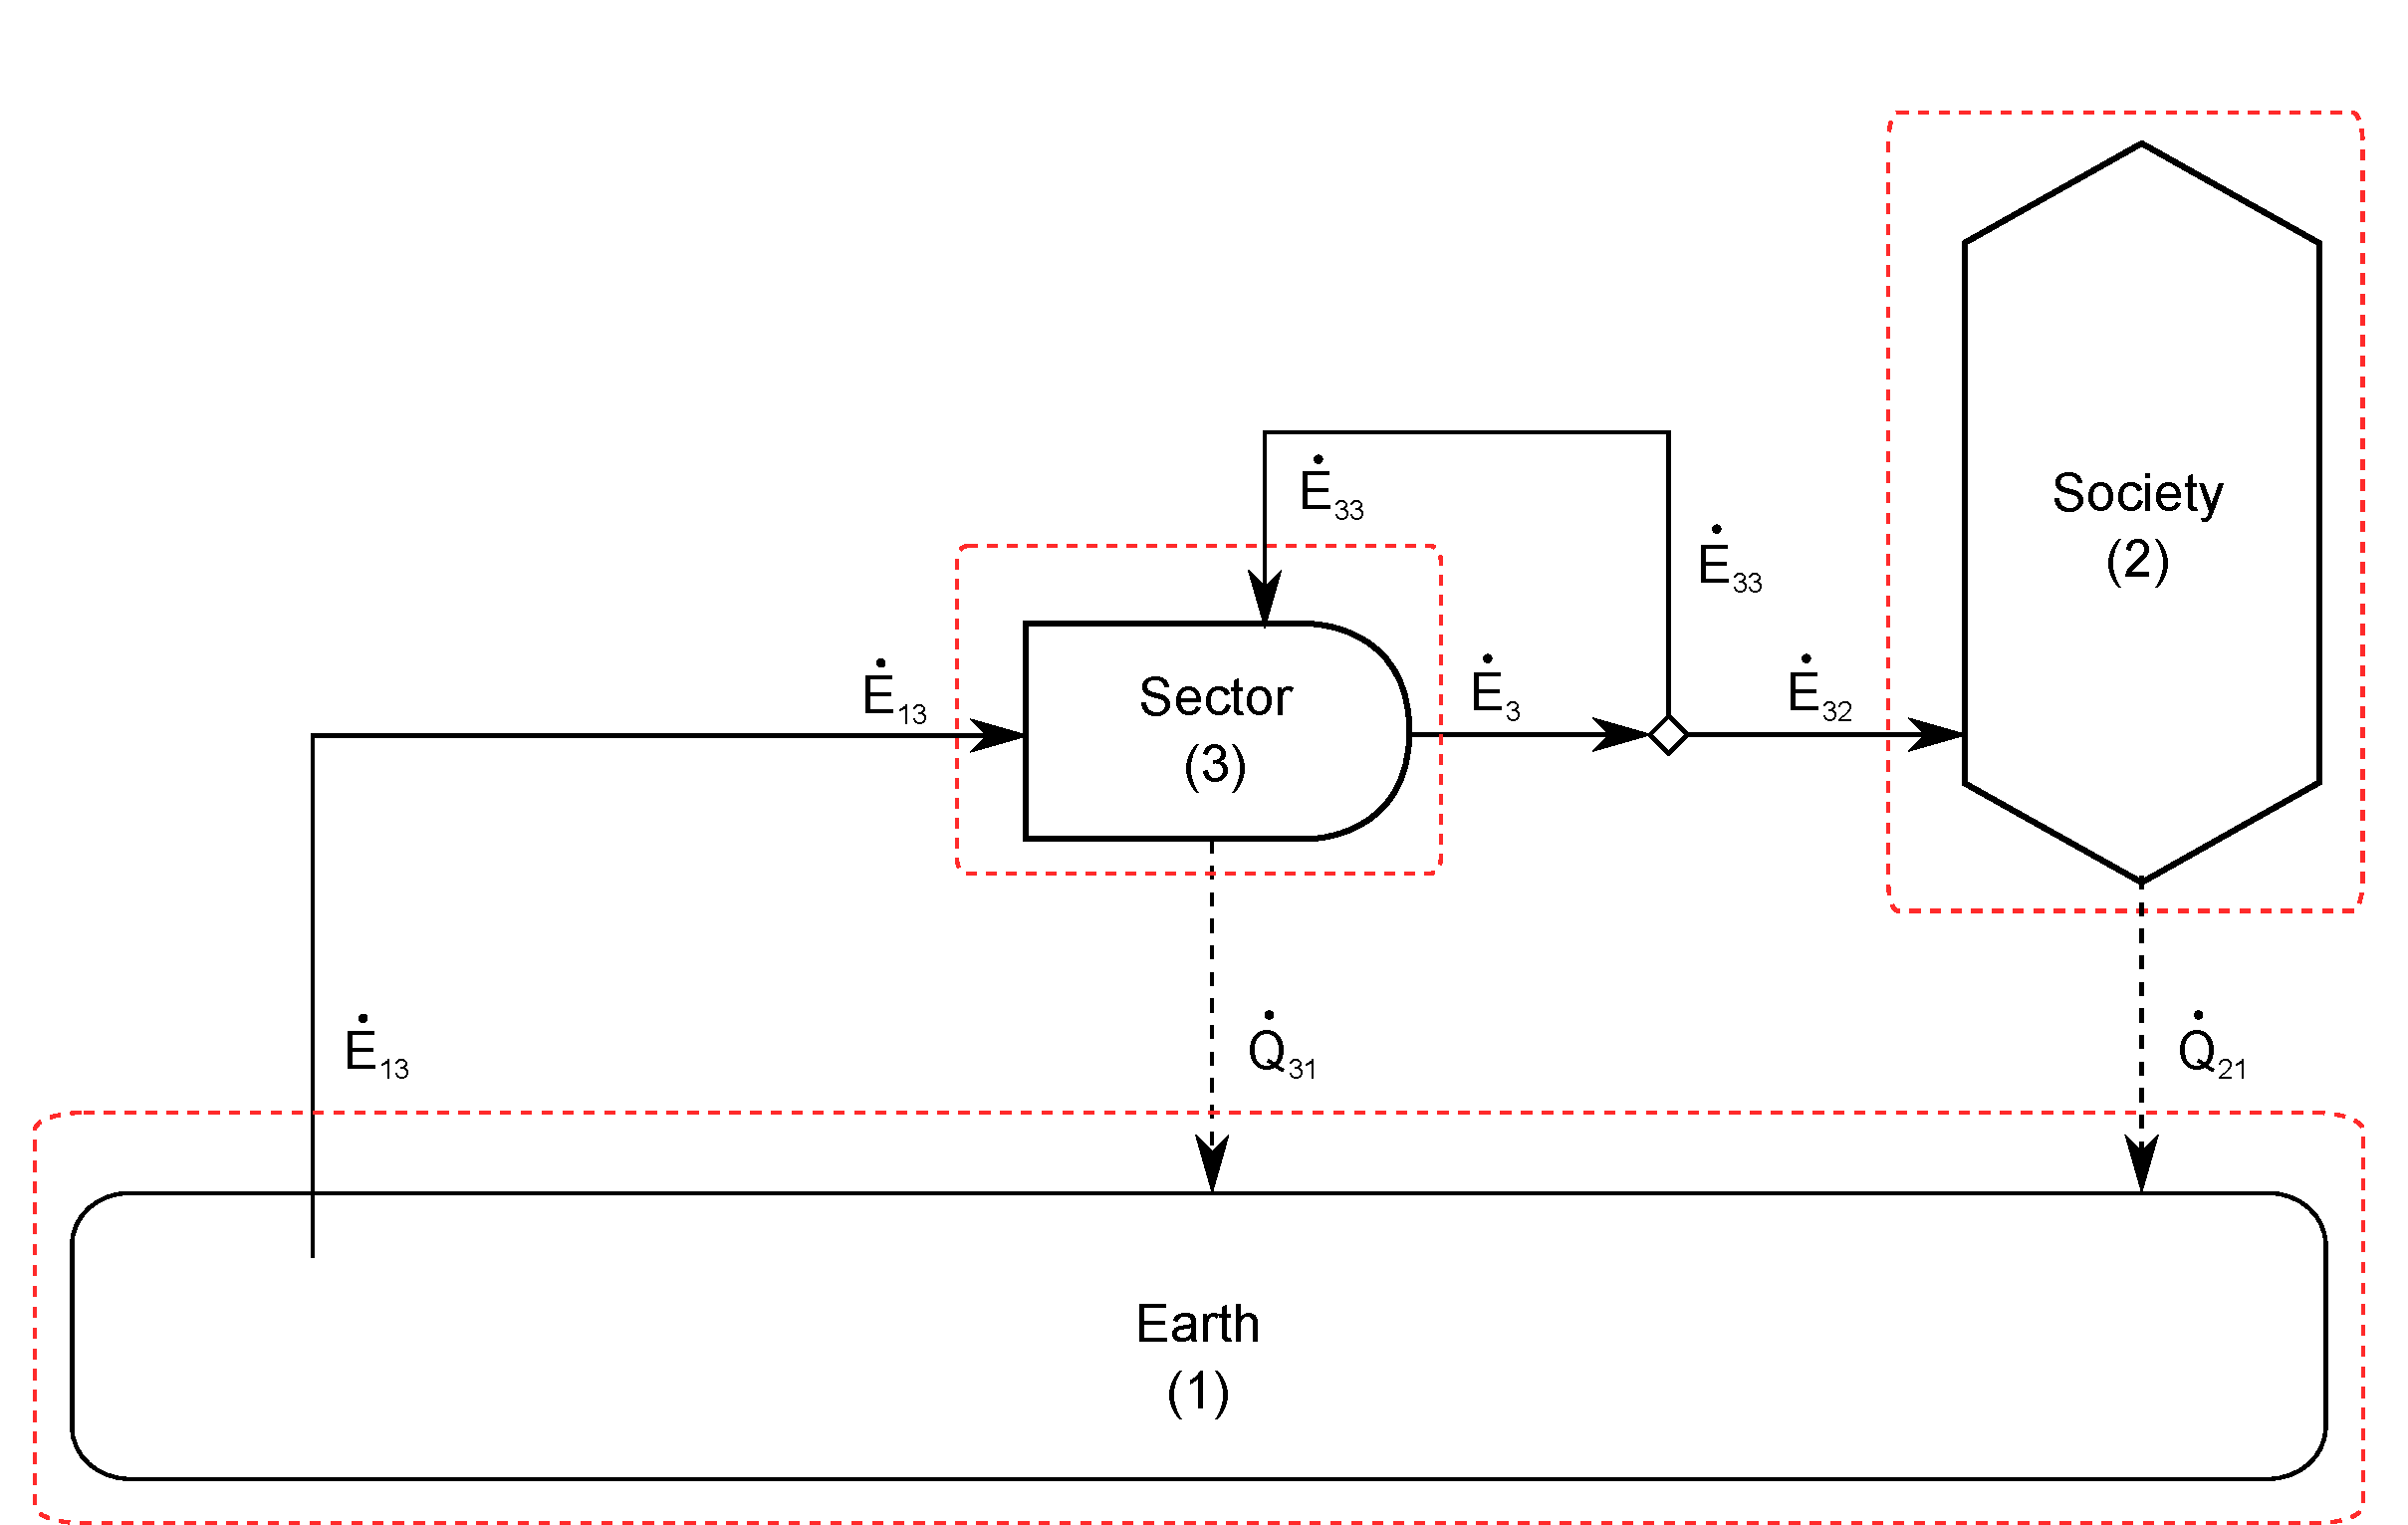
\includegraphics[width=1.0\linewidth]{Chapter_Example_B/images/I-O_two_sector_direct_energy.pdf}
\caption{Flows of direct energy ($\dot{E}$) and waste heat ($\dot{Q}$) in a one-sector economy with separate demand.}
\label{fig:direct_energy_flows}
\end{figure}

The First Law around the economic Sector (3) including the accumulation rate of direct energy in the sector $\left(\frac{\mathrm{d}E_{3}}{\mathrm{d}t}\right)$ yields

\begin{equation} \label{eq:CV_E_dot_3}
	\frac{\mathrm{d}E_{3}}{\mathrm{d}t} 	 = \dot{E}_{13} + \dot{E}_{33} - \dot{E}_{3} - \dot{Q}_{31}.
\end{equation}

\noindent It is notable that the economic Sector (3) consumes a portion of its own energy output ($\dot{E}_{33}$) as it produces its goods and services: it takes energy to make energy.

First Law energy accounting around the Earth (1) and Society (2) gives

\begin{equation} \label{eq:CV_E_dot_1}
	\frac{\mathrm{d}E_{1}}{\mathrm{d}t} 	 =  \dot{Q}_{21} + \dot{Q}_{31} - \dot{E}_{13},
\end{equation}

\noindent and 

\begin{equation} \label{eq:CV_E_dot_2}
	\frac{\mathrm{d}E_{2}}{\mathrm{d}t} 	 = \dot{E}_{32} - \dot{Q}_{21}.
\end{equation}

As in Example A, we can set the accumulation of direct energy within each sector to zero to obtain

\begin{equation} \label{eq:CV_E_dot_3_SS}
	0 =\dot{E}_{13} + \dot{E}_{33} - \dot{E}_{3} - \dot{Q}_{31},
\end{equation}

\begin{equation} \label{eq:CV_E_dot_1_SS}
	0 =  \dot{Q}_{21} + \dot{Q}_{31} - \dot{E}_{13},
\end{equation}

\noindent and 

\begin{equation} \label{eq:CV_E_dot_2_SS}
	0 =\dot{E}_{32} - \dot{Q}_{21},
\end{equation}

%%%%%%%%%%% Example B %%%%%%%%%%
%\section{Energy ratios}
%%%%%%%%%%%
%
%[IS THERE ANY POINT IN DEFINING THESE HERE IF THEY ARE NOT USED? I HAVE COMMENTED THEM OUT AS I THINK THEY HAVE BEEN MOVED TO LATER SECTION IN EXAMPLE C - MD]
%
%Several important energy ratios can be observed in Figure \ref{fig:direct_energy_flows}. The Gross Energy Ratio ($GER$) is defined as 
%
%\begin{equation} \label{eq:GER_def_ch_5}
%	GER \equiv \frac{\dot{E}_{3}}{\dot{E}_{33}}.
%\end{equation}
%
%\noindent The Net Energy Ratio ($NER$) is defined as
%
%\begin{equation} \label{eq:NER_def_ch_5}
%	NER \equiv \frac{\dot{E}_{32}}{\dot{E}_{33}} = GER - 1.
%\end{equation}
%
%[THESE DEFINITIONS ARE EQUIVALENT TO $\beta$ BOUNDARY DEFINED IN BRANDT AND DALE (2011). WE CANNOT DISTINGUISH EXTERNAL ENERGY RATIOS AT THIS POINT. NOT SURE ABOUT COMMENTED WORK BELOW - CHECK TEX FILE.]

%The rate of energy extracted from the Earth can be expressed as either
%
%\begin{equation} \label{eq:E_dot_13_a}
%	\dot{E}_{13} = \frac{GER - 1}{NEER}\dot{E}_{22}
%\end{equation}
%
%\noindent or
%
%\begin{equation} \label{eq:E_dot_32_b}
%	\dot{E}_{32} = \frac{1 - \frac{1}{GER}}{NEER}\dot{E}_{2}.
%\end{equation}

%%%%%%%%%% Example B %%%%%%%%%%
\section{Total energy accounting}
%%%%%%%%%%

Again, we follow the I-O literature in assuming that total energy (i.e., the sum of direct energy and indirect energy) is conserved. Thus, we can draw a diagram similar to Figure \ref{fig:direct_energy_flows} for total energy flows. See Figure \ref{fig:total_energy_flows_1S}.

\begin{figure}[h!]
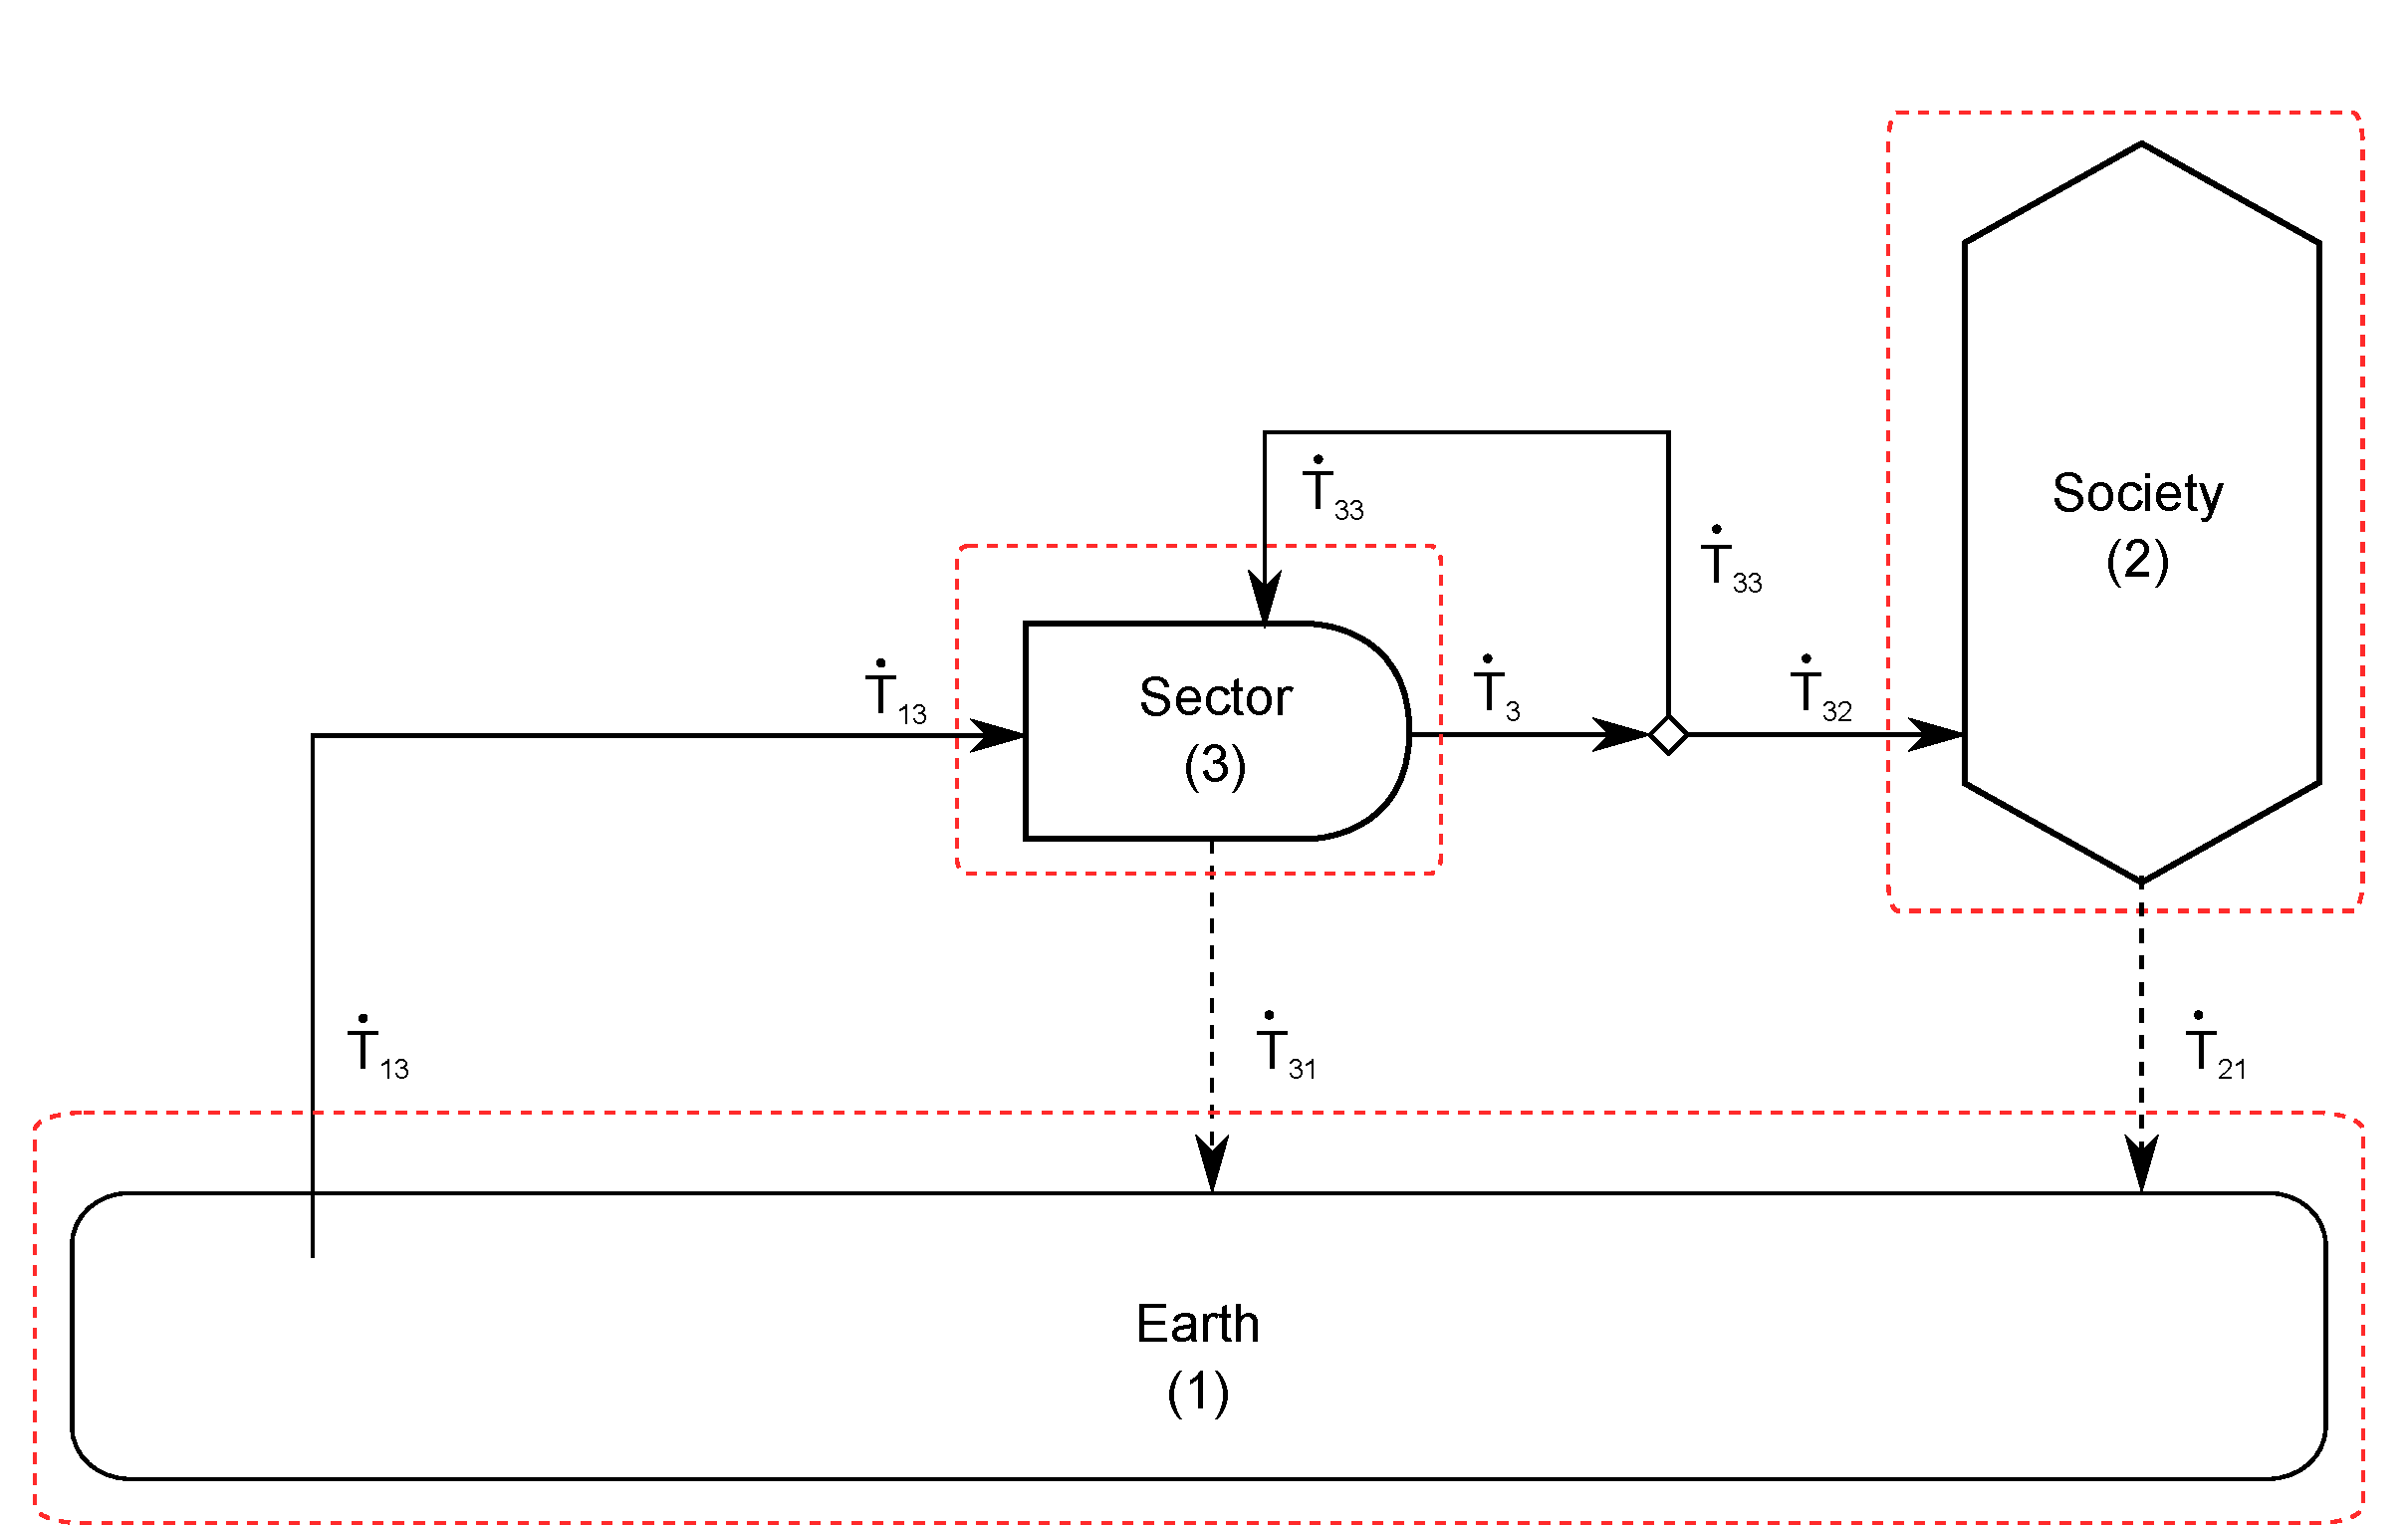
\includegraphics[width=1.0\linewidth]{Chapter_Example_B/images/I-O_two_sector_total_energy.pdf}
\caption{Flows of total energy ($\dot{T}$) in a one-sector economy with separate demand.}
\label{fig:total_energy_flows_1S}
\end{figure}

Accounting for accumulation of total energy and using the assumption that total energy is conserved, we can write the following equations.

\begin{equation} \label{eq:CV_T_1}
	\frac{\mathrm{d}T_{1}}{\mathrm{d}t} 	 = \dot{T}_{21} + \dot{T}_{31} - \dot{T}_{13},
\end{equation}

\begin{equation} \label{eq:CV_T_2}
	\frac{\mathrm{d}T_{2}}{\mathrm{d}t} 	 = \dot{T}_{32} - \dot{T}_{21},
\end{equation}

\noindent and

\begin{equation} \label{eq:CV_T_3}
	\frac{\mathrm{d}T_{3}}{\mathrm{d}t} 	 = \dot{T}_{13} + \dot{T}_{33} - \dot{T}_{3} - \dot{T}_{31}.
\end{equation}

%%%%%%%%%% Example B %%%%%%%%%%
\section{Embodied energy accounting}
%%%%%%%%%%

Given that $\frac{\mathrm{d}E_{i}}{\mathrm{d}t} = 0$ and $\dot{T} = \dot{E} + \dot{B}$, we note that

\begin{equation} \label{eq:T_dot_equals_B_dot}
	\frac{\mathrm{d}T_i}{\mathrm{d}t} = \frac{\mathrm{d}B_i}{\mathrm{d}t},
\end{equation}

\noindent and we can rewrite the total energy accumulation accounting equations as

\begin{equation} \label{eq:CV_dB_1}
	\frac{\mathrm{d}B_{1}}{\mathrm{d}t} = \dot{E}_{21} + \dot{B}_{21} + \dot{E}_{31} + \dot{B}_{31} - \dot{E}_{13} + \dot{B}_{13},
\end{equation}

\begin{equation} \label{eq:CV_dB_2}
	\frac{\mathrm{d}B_{2}}{\mathrm{d}t} = \dot{E}_{32} + \dot{B}_{32} - \dot{E}_{21} - \dot{B}_{21},
\end{equation}

\noindent and 

\begin{equation} \label{eq:CV_dB_3}
	\frac{\mathrm{d}B_{3}}{\mathrm{d}t} = \dot{E}_{13} + \dot{B}_{13} + \dot{E}_{33} + \dot{B}_{33} - \dot{E}_{3} - \dot{B}_{3} - \dot{E}_{31} - \dot{B}_{31}.
\end{equation}

As in Example A, we can substitute the First Law of Thermodynamics for the economic Sector (Equation \ref{eq:CV_E_dot_3_SS}) into the total energy accounting equation for the economic Sector (Equation \ref{eq:CV_dB_3}). Assuming that $\dot{E}_{31} = 0$ (because energy is returned to the Earth as waste heat, not direct energy), we obtain

\begin{equation} \label{eq:ExB_embodied_energy_accounting}
	\frac{\mathrm{d}B_3}{\mathrm{d}t} = \dot{Q}_{31} + \dot{B}_{13} + \dot{B}_{33} - \dot{B}_{31}
\end{equation}

Similar to Example A, we observe that the accumulation rate of embodied energy in the Goods and Services sector (3) is the sum of the rates of waste heat from the sector ($\dot{Q}_{31}$) and embodied energy into the sector ($\dot{B}_{13} + \dot{B}_{33}$) less the rate of embodied energy leaving the sector on its output stream ($\dot{B}_{31}$).

%%%%%%%%%% Example B %%%%%%%%%%
\section{Depreciation}
%%%%%%%%%%

We can substitute a depreciation term for the flow rate of embodied energy from the economic Sector (3) to the Earth (1) to obtain

\begin{equation} \label{eq:ExB_embodied_energy_accounting_with_depreciation}
	\frac{\mathrm{d}B_3}{\mathrm{d}t} = \dot{Q}_{31} + \dot{B}_{13} + \dot{B}_{33} - \gamma_3 B_3.
\end{equation}

%%%%%%%%%% Example B %%%%%%%%%%
\section{Estimating energy intensity ($\varepsilon$) of the economy}
%%%%%%%%%%

The following figure shows value flows ($\dot{X}$) in the one-sector economy with separate demand.

\begin{figure}[H]
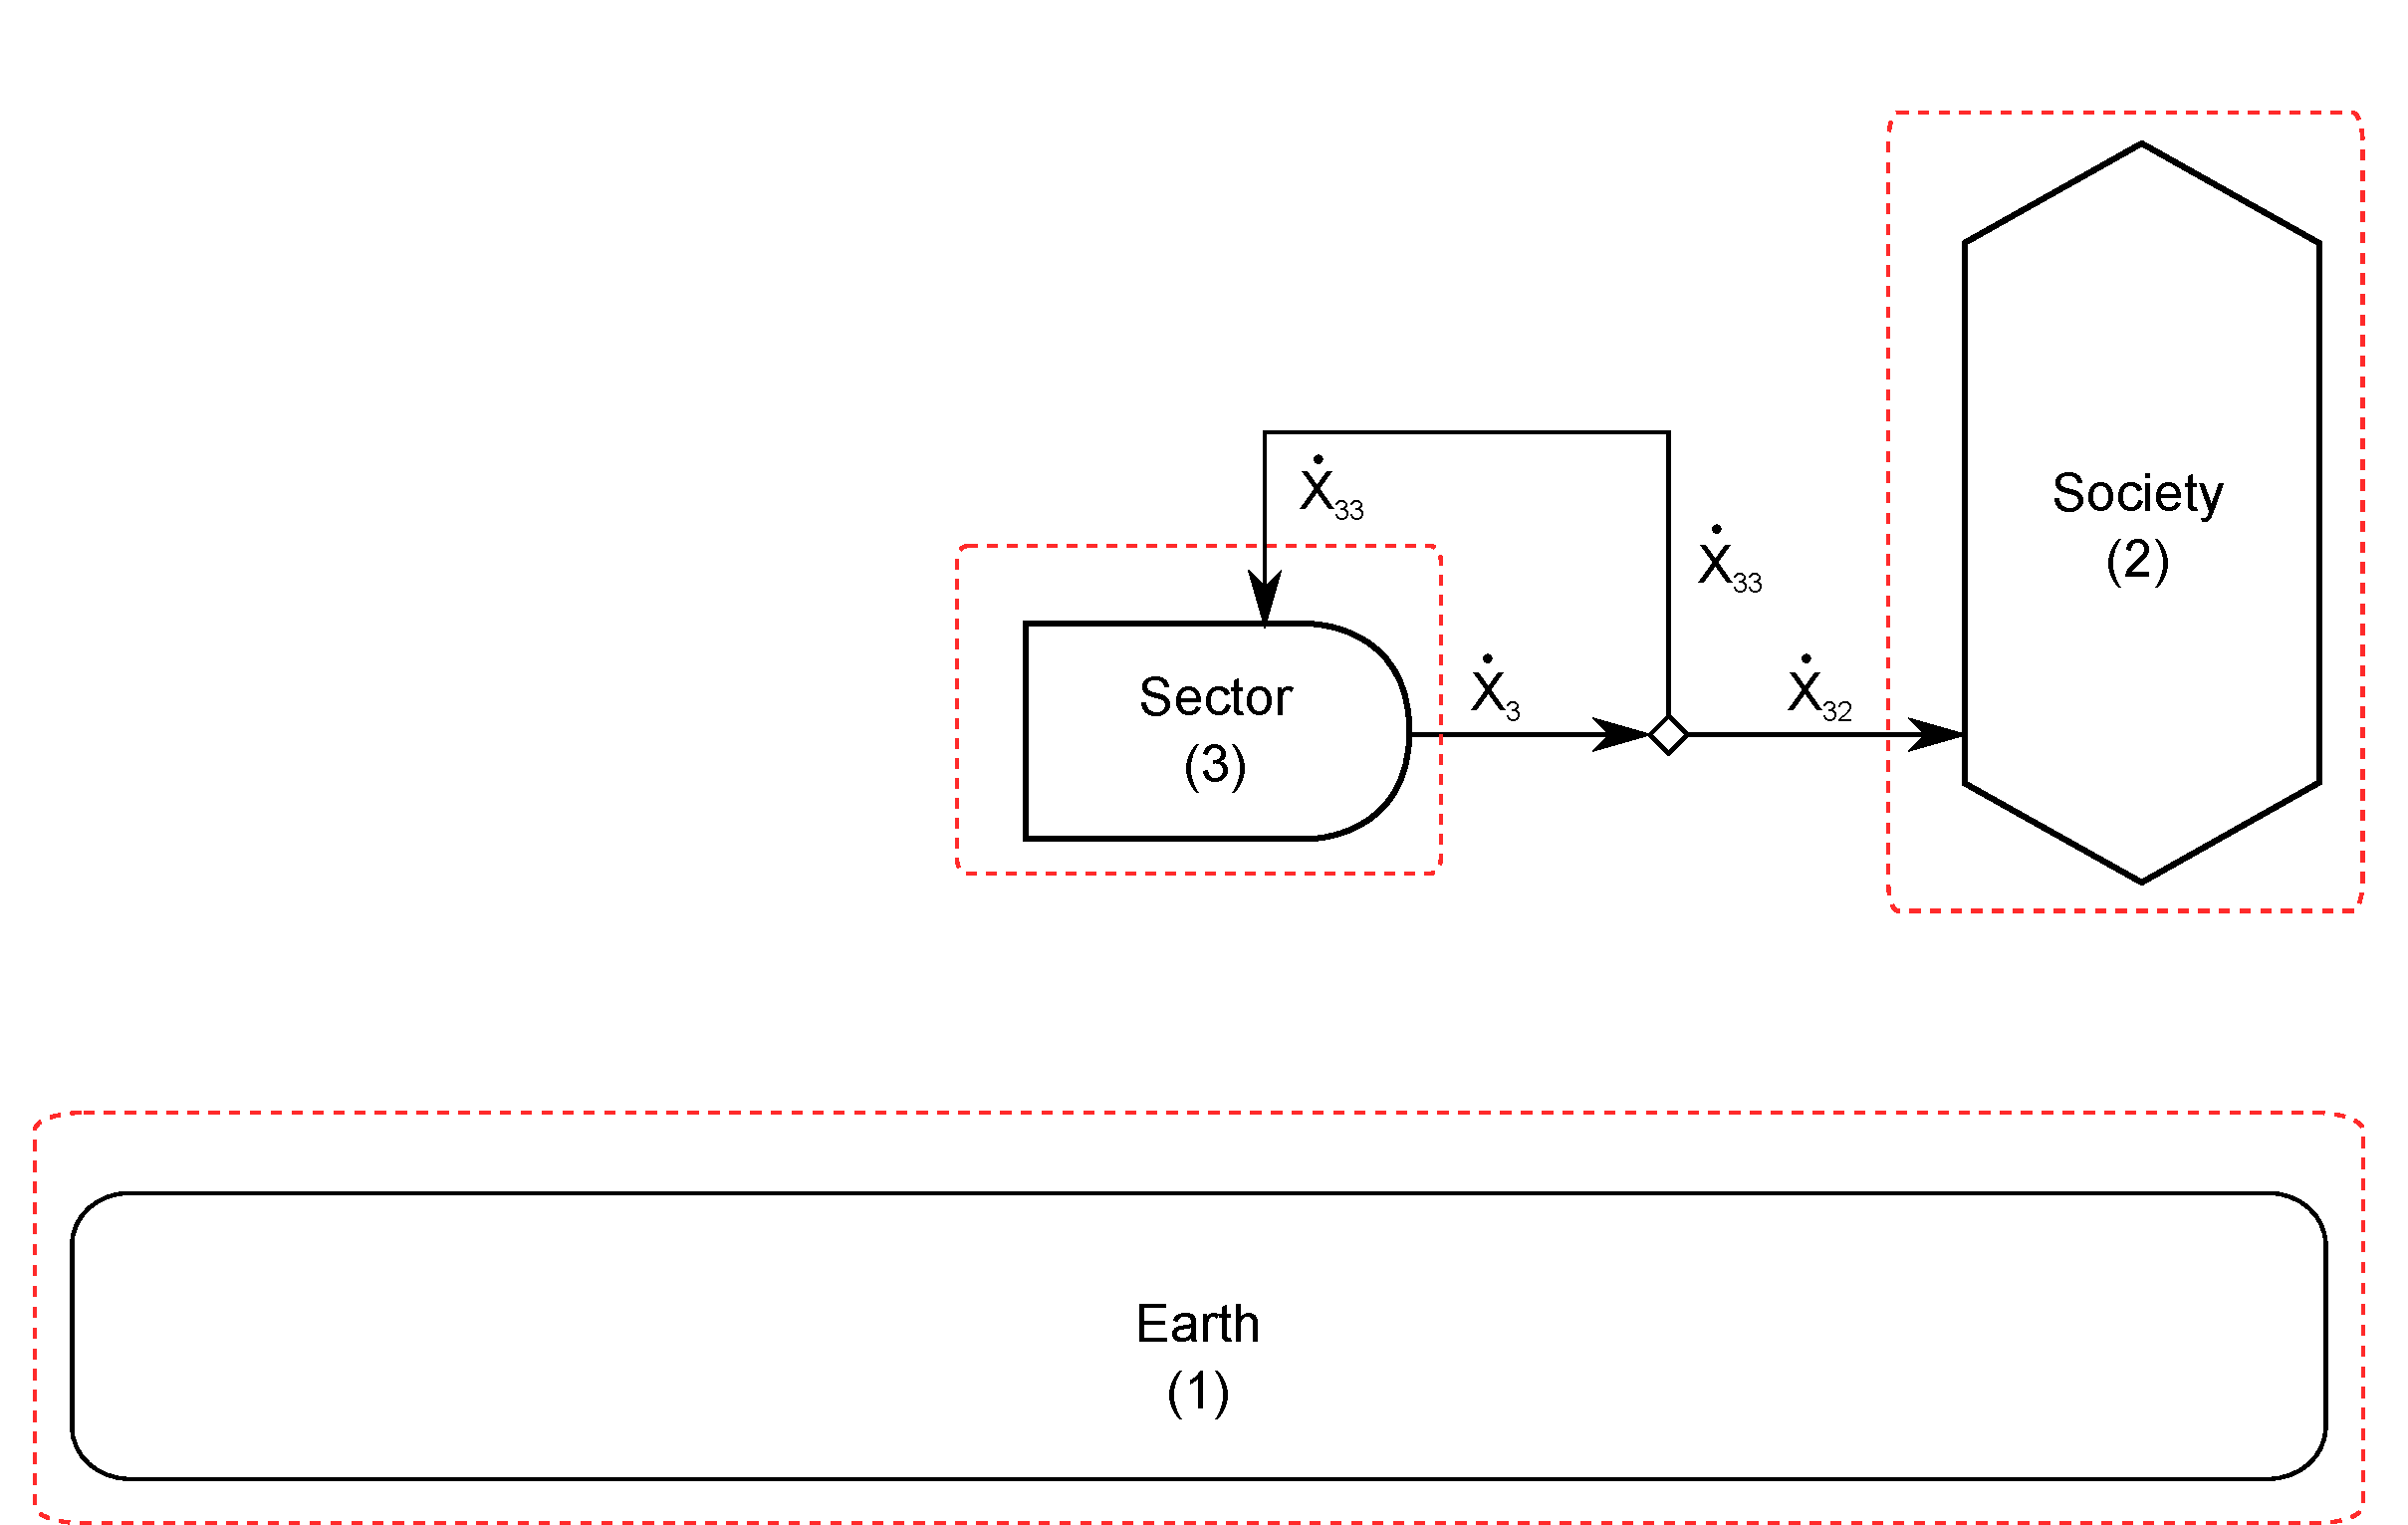
\includegraphics[width=1.0\linewidth]{Chapter_Example_B/images/I-O_two_sector_value.pdf}
\caption{Flows of economic value ($\dot{X}$) in a one-sector economy with separate demand.}
\label{fig:economic_value_flows}
\end{figure}

The energy intensity ($\varepsilon$) of the economic Sector (3) is given by

\begin{equation} \label{eq:single_sector_energy_intensity}
	\varepsilon_{3} = \frac{\dot{T}_{3}}{\dot{X}_{3}} = \frac{\dot{T}_{33}}{\dot{X}_{33}}.
\end{equation}

The input-output ratio ($a$) for the economic Sector (3) is

\begin{equation} \label{eq:io_ratio_single_sector}
	a_{33} = \frac{\dot{X}_{33}}{\dot{X}_{3}}.
\end{equation}

\noindent Thus,

\begin{equation} \label{eq:T_dot_1_single_sector}
	\dot{T}_{3} = \varepsilon_{3}\dot{X}_{3},
\end{equation}

\noindent and

\begin{equation} \label{eq:T_dot_11_single_sector}
	\dot{T}_{33} = \varepsilon_{3}a_{33}\dot{X}_{3}.
\end{equation}

Realizing that (a) $\frac{\mathrm{d}T_3}{\mathrm{d}t} = \frac{\mathrm{d}B_3}{\mathrm{d}t}$ because $\frac{\mathrm{d}E_3}{\mathrm{d}t} = 0$, (b) $\dot{T}_{13} = \dot{E}_{13}$ because $\dot{B}_{13} = 0$ due to processing of raw energy carriers occurring \emph{within} the economic Sector (3), and (c) substituting Equations \ref{eq:T_dot_1_single_sector} and \ref{eq:T_dot_11_single_sector} into Equation \ref{eq:CV_T_3} gives

\begin{equation} \label{eq:dB1/dt_single_sector_after_substituting_eps_and_a}
	\frac{\mathrm{d}B_{3}}{\mathrm{d}t} = \varepsilon_{3}a_{33}\dot{X}_{3} + \dot{E}_{13} - \varepsilon_{3}\dot{X}_{3} - \gamma_{3}B_{3}.
\end{equation}

We can estimate the energy intensity of the economy by solving Equation \ref{eq:dB1/dt_single_sector_after_substituting_eps_and_a} for $\varepsilon_{3}$.

\begin{equation} \label{eq:eps3_ss_IO}
	\varepsilon_{3} = (1 - a_{33})^{-1} \dot{X}_{3}^{-1} \left[\dot{E}_{13} - \left(\frac{\mathrm{d}B_{3}}{\mathrm{d}t} + \gamma_{3}B_{3}\right)\right]
\end{equation}

Equation \ref{eq:eps3_ss_IO} is similar to the typical energy intensity equation found in the I-O literature [REFERENCE BULLARD AND OTHERS HERE. --MKH], except that Equation \ref{eq:eps3_ss_IO} applies to a single economic sector and contains scalar (as opposed to matrix) terms. Using Example C below, we will derive a matrix representation of Equation \ref{eq:eps3_ss_IO} that is directly comparable to energy intensity equations found in the I-O literature.

%%%%%%%%% Example B %%%%%%%%%%
\section{Derivation of economic sector energy intensity ($\varepsilon$) by a convergent infinite series}
%%%%%%%%%%

The single-sector economy of Figures \ref{fig:direct_energy_flows} through \ref{fig:economic_value_flows} can be re-drawn as shown in Figure \ref{fig:single_sector_flows_3}.

\begin{figure}[h!]
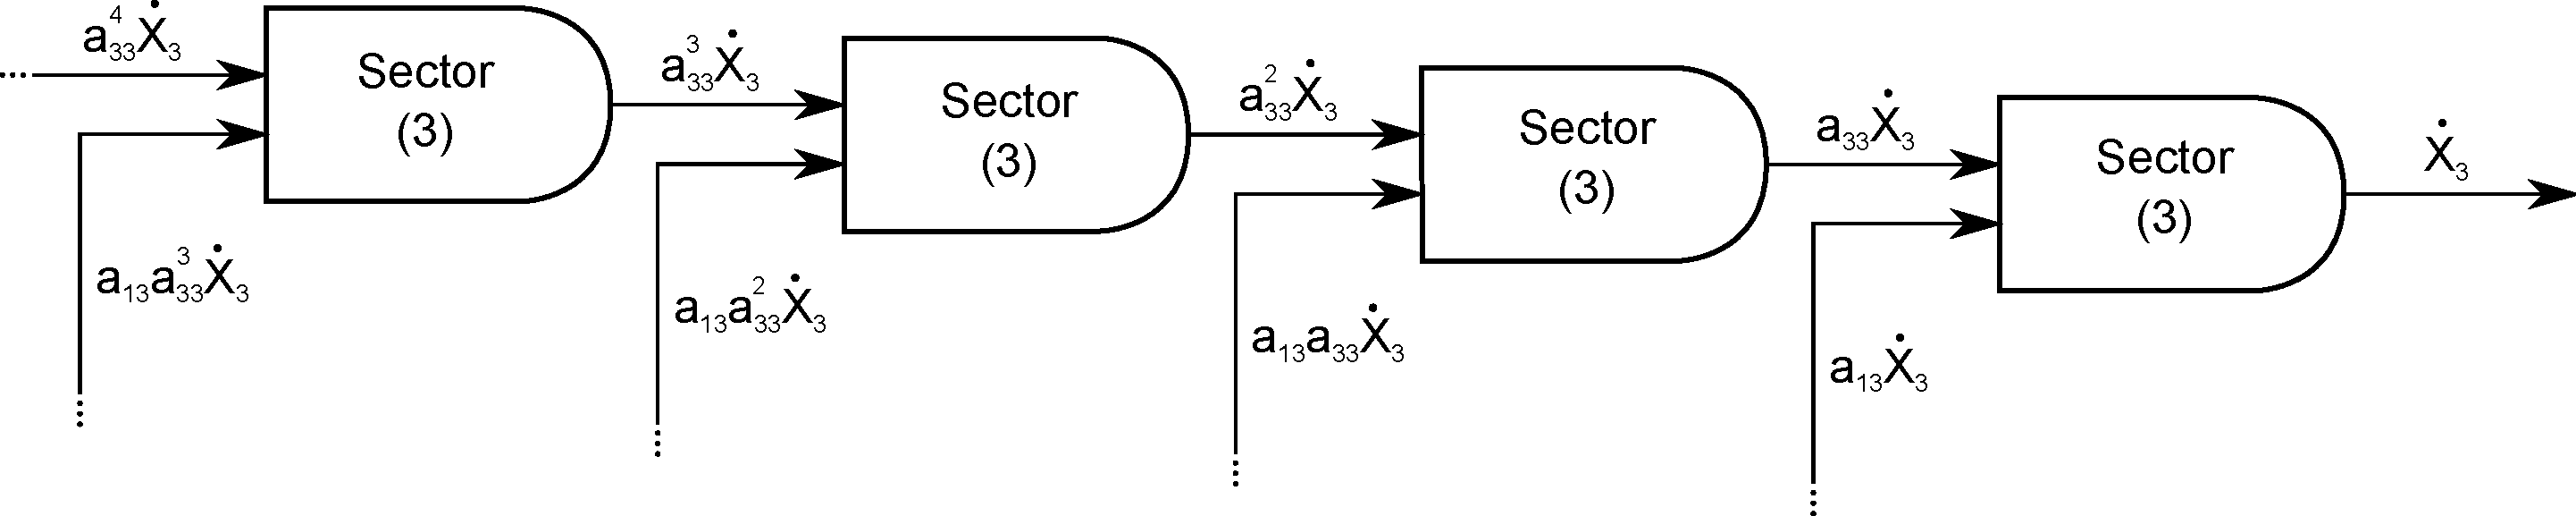
\includegraphics[width=1.0\linewidth]{Chapter_Example_B/images/Heun_I-O_Process_Equivalence_3.pdf}
\caption{Process flows in a single-sector economy.}
\label{fig:single_sector_flows_3}
\end{figure}

The economy produces output at a rate of $\dot{X}_{3}$, but it requires energy from the Earth ($\dot{E}_{13} = a_{13}\dot{X}_{3}$) to do so. The economy also consumes a fraction of its own gross output ($\dot{X}_{33} = a_{33}\dot{X}_{3}$). To produce $a_{33}\dot{X}_{3}$, the economy requires an additional $a_{13}a_{33}\dot{X}_{3}$ of energy from the Earth. The total energy required for the economy to produce at a rate of $\dot{X}_{3}$ is an infinite sum.

\begin{equation} \label{eq:E_dot_demand_SS}
	\dot{E}_{demand} = a_{13}\dot{X}_{3} + a_{13}a_{33}\dot{X}_{3} + a_{13}a_{33}^2\dot{X}_{3} + \cdots
\end{equation}

The energy intensity of the economy ($\varepsilon_{3}$) is 

\begin{equation} \label{eq:epsilon_process_SS_intermediate}
	\varepsilon_{3} = \frac{\dot{E}_{demand}}{\dot{X}_{3}} = a_{13}(1 + a_{33} + a_{33}^2) + \cdots = a_{13}\sum_{n=0}^{\infty}a_{33}^{n}.
\end{equation}

Realizing that $\sum_{n=0}^{\infty}a_{33}^{n} = \frac{1}{1-a_{33}}$ and $a_{13} = \frac{\dot{E}_{13}}{\dot{X}_{3}}$ gives

\begin{equation} \label{eq:epsilon_process_SS}
	\varepsilon_{1} = (1-a_{33})^{-1} \dot{X}^{-1} \dot{E}_{13}.
\end{equation}

Neglecting accumulation of embodied energy in the economy $\left(\frac{\mathrm{d}B_{3}}{\mathrm{d}t}\right)$ and depreciation $\left(\gamma_{3}B_{3}\right)$, Equations \ref{eq:eps3_ss_IO} and \ref{eq:epsilon_process_SS} are identical (assuming $\frac{\mathrm{d}B_{3}}{\mathrm{d}t} =\gamma_{3} = 0$), indicating that the I-O approach accounts for the infinite recursion of energy demand by the economy.




\bibliography{EROI_review_v2}
\bibliographystyle{unsrt}


% Always give a unique label
% and use \ref{<label>} for cross-references
% and \cite{<label>} for bibliographic references
% use \sectionmark{}
% to alter or adjust the section heading in the running head
%% Instead of simply listing headings of different levels we recommend to let every heading be followed by at least a short passage of text. Furtheron please use the \LaTeX\ automatism for all your cross-references and citations.

%% Please note that the first line of text that follows a heading is not indented, whereas the first lines of all subsequent paragraphs are.

%% Use the standard \verb|equation| environment to typeset your equations, e.g.
%
%% \begin{equation}
%% a \times b = c\;,
%% \end{equation}
%
%% however, for multiline equations we recommend to use the \verb|eqnarray|
%% environment\footnote{In physics texts please activate the class option \texttt{vecphys} to depict your vectors in \textbf{\itshape boldface-italic} type - as is customary for a wide range of physical subjects.}.
%% \begin{eqnarray}
%% a \times b = c \nonumber\\
%% \vec{a} \cdot \vec{b}=\vec{c}
%% \label{eq:01}
%% \end{eqnarray}

%% \subsection{Subsection Heading}
%% \label{subsec:2}
%% Instead of simply listing headings of different levels we recommend to let every heading be followed by at least a short passage of text. Furtheron please use the \LaTeX\ automatism for all your cross-references\index{cross-references} and citations\index{citations} as has already been described in Sect.~\ref{sec:2}.

%% \begin{quotation}
%% Please do not use quotation marks when quoting texts! Simply use the \verb|quotation| environment -- it will automatically render Springer's preferred layout.
%% \end{quotation}


%% \subsubsection{Subsubsection Heading}
%% Instead of simply listing headings of different levels we recommend to let every heading be followed by at least a short passage of text. Furtheron please use the \LaTeX\ automatism for all your cross-references and citations as has already been described in Sect.~\ref{subsec:2}, see also Fig.~\ref{fig:1}\footnote{If you copy text passages, figures, or tables from other works, you must obtain \textit{permission} from the copyright holder (usually the original publisher). Please enclose the signed permission with the manucript. The sources\index{permission to print} must be acknowledged either in the captions, as footnotes or in a separate section of the book.}

%% Please note that the first line of text that follows a heading is not indented, whereas the first lines of all subsequent paragraphs are.

% For figures use
%
%% \begin{figure}[b]
%% \sidecaption
% Use the relevant command for your figure-insertion program
% to insert the figure file.
% For example, with the option graphics use
%% \includegraphics[scale=.65]{figure}
%
% If not, use
%\picplace{5cm}{2cm} % Give the correct figure height and width in cm
%
%% \caption{If the width of the figure is less than 7.8 cm use the \texttt{sidecapion} command to flush the caption on the left side of the page. If the figure is positioned at the top of the page, align the sidecaption with the top of the figure -- to achieve this you simply need to use the optional argument \texttt{[t]} with the \texttt{sidecaption} command}
%% \label{fig:1}       % Give a unique label
%% \end{figure}


%% \paragraph{Paragraph Heading} %
%% Instead of simply listing headings of different levels we recommend to let every heading be followed by at least a short passage of text. Furtheron please use the \LaTeX\ automatism for all your cross-references and citations as has already been described in Sect.~\ref{sec:2}.

%% Please note that the first line of text that follows a heading is not indented, whereas the first lines of all subsequent paragraphs are.

%% For typesetting numbered lists we recommend to use the \verb|enumerate| environment -- it will automatically render Springer's preferred layout.

%% \begin{enumerate}
%% \item{Livelihood and survival mobility are oftentimes coutcomes of uneven socioeconomic development.}
%% \begin{enumerate}
%% \item{Livelihood and survival mobility are oftentimes coutcomes of uneven socioeconomic development.}
%% \item{Livelihood and survival mobility are oftentimes coutcomes of uneven socioeconomic development.}
%% \end{enumerate}
%% \item{Livelihood and survival mobility are oftentimes coutcomes of uneven socioeconomic development.}
%% \end{enumerate}


%% \subparagraph{Subparagraph Heading} In order to avoid simply listing headings of different levels we recommend to let every heading be followed by at least a short passage of text. Use the \LaTeX\ automatism for all your cross-references and citations as has already been described in Sect.~\ref{sec:2}, see also Fig.~\ref{fig:2}.

%% Please note that the first line of text that follows a heading is not indented, whereas the first lines of all subsequent paragraphs are.

%% For unnumbered list we recommend to use the \verb|itemize| environment -- it will automatically render Springer's preferred layout.

%% \begin{itemize}
%% \item{Livelihood and survival mobility are oftentimes coutcomes of uneven socioeconomic development, cf. Table~\ref{tab:1}.}
%% \begin{itemize}
%% \item{Livelihood and survival mobility are oftentimes coutcomes of uneven socioeconomic development.}
%% \item{Livelihood and survival mobility are oftentimes coutcomes of uneven socioeconomic development.}
%% \end{itemize}
%% \item{Livelihood and survival mobility are oftentimes coutcomes of uneven socioeconomic development.}
%% \end{itemize}

%% \begin{figure}[t]
%% \sidecaption[t]
% Use the relevant command for your figure-insertion program
% to insert the figure file.
% For example, with the option graphics use
%% \includegraphics[scale=.65]{figure}
%
% If not, use
%\picplace{5cm}{2cm} % Give the correct figure height and width in cm
%
%% \caption{Please write your figure caption here}
%% \label{fig:2}       % Give a unique label
%% \end{figure}

%% \runinhead{Run-in Heading Boldface Version} Use the \LaTeX\ automatism for all your cross-references and citations as has already been described in Sect.~\ref{sec:2}.

%% \subruninhead{Run-in Heading Italic Version} Use the \LaTeX\ automatism for all your cross-refer\-ences and citations as has already been described in Sect.~\ref{sec:2}\index{paragraph}.
% Use the \index{} command to code your index words
%
% For tables use
%
%% \begin{table}
%% \caption{Please write your table caption here}
%% \label{tab:1}       % Give a unique label
%
% For LaTeX tables use
%
%% \begin{tabular}{p{2cm}p{2.4cm}p{2cm}p{4.9cm}}
%% \hline\noalign{\smallskip}
%% Classes & Subclass & Length & Action Mechanism  \\
%% \noalign{\smallskip}\svhline\noalign{\smallskip}
%% Translation & mRNA$^a$  & 22 (19--25) & Translation repression, mRNA cleavage\\
%% Translation & mRNA cleavage & 21 & mRNA cleavage\\
%% Translation & mRNA  & 21--22 & mRNA cleavage\\
%%Translation & mRNA  & 24--26 & Histone and DNA Modification\\
%%\noalign{\smallskip}\hline\noalign{\smallskip}
%%\end{tabular}
%%$^a$ Table foot note (with superscript)
%%\end{table}
%
%% \section{Section Heading}
%%\label{sec:3}
% Always give a unique label
% and use \ref{<label>} for cross-references
% and \cite{<label>} for bibliographic references
% use \sectionmark{}
% to alter or adjust the section heading in the running head
%% Instead of simply listing headings of different levels we recommend to let every heading be followed by at least a short passage of text. Furtheron please use the \LaTeX\ automatism for all your cross-references and citations as has already been described in Sect.~\ref{sec:2}.

%% Please note that the first line of text that follows a heading is not indented, whereas the first lines of all subsequent paragraphs are.

%%If you want to list definitions or the like we recommend to use the Springer-enhanced \verb|description| environment -- it will automatically render Springer's preferred layout.

%%\begin{description}[Type 1]
%%\item[Type 1]{That addresses central themes pertainng to migration, health, and disease. In Sect.~\ref{sec:1}, Wilson discusses the role of human migration in infectious disease distributions and patterns.}
%%\item[Type 2]{That addresses central themes pertainng to migration, health, and disease. In Sect.~\ref{subsec:2}, Wilson discusses the role of human migration in infectious disease distributions and patterns.}
%%\end{description}

%%\subsection{Subsection Heading} %
%% In order to avoid simply listing headings of different levels we recommend to let every heading be followed by at least a short passage of text. Use the \LaTeX\ automatism for all your cross-references and citations citations as has already been described in Sect.~\ref{sec:2}.

%% Please note that the first line of text that follows a heading is not indented, whereas the first lines of all subsequent paragraphs are.

%% \begin{svgraybox}
%% If you want to emphasize complete paragraphs of texts we recommend to use the newly defined Springer class option \verb|graybox| and the newly defined environment \verb|svgraybox|. This will produce a 15 percent screened box 'behind' your text.

%% If you want to emphasize complete paragraphs of texts we recommend to use the newly defined Springer class option and environment \verb|svgraybox|. This will produce a 15 percent screened box 'behind' your text.
%% \end{svgraybox}


%% \subsubsection{Subsubsection Heading}
%%Instead of simply listing headings of different levels we recommend to let every heading be followed by at least a short passage of text. Furtheron please use the \LaTeX\ automatism for all your cross-references and citations as has already been described in Sect.~\ref{sec:2}.

%% Please note that the first line of text that follows a heading is not indented, whereas the first lines of all subsequent paragraphs are.

%% \begin{theorem}
%% Theorem text goes here.
%% \end{theorem}
%
% or
%
%% \begin{definition}
%% Definition text goes here.
%% \end{definition}

%% \begin{proof}
%\smartqed
%% Proof text goes here.
%% \qed
%% \end{proof}

%%\paragraph{Paragraph Heading} %
%% Instead of simply listing headings of different levels we recommend to let every heading be followed by at least a short passage of text. Furtheron please use the \LaTeX\ automatism for all your cross-references and citations as has already been described in Sect.~\ref{sec:2}.

%% Note that the first line of text that follows a heading is not indented, whereas the first lines of all subsequent paragraphs are.
%
% For built-in environments use
%
%%\begin{theorem}
%%Theorem text goes here.
%%\end{theorem}
%
%%\begin{definition}
%%Definition text goes here.
%%\end{definition}
%
%%\begin{proof}
%%\smartqed
%% Proof text goes here.
%%\qed
%%\end{proof}
%
%% \begin{acknowledgement}
%% If you want to include acknowledgments of assistance and the like at the end of an individual chapter please use the \verb|acknowledgement| environment -- it will automatically render Springer's preferred layout.
%% \end{acknowledgement}
%
%% \section*{Appendix}
%% \addcontentsline{toc}{section}{Appendix}
%
%% When placed at the end of a chapter or contribution (as opposed to at the end of the book), the numbering of tables, figures, and equations in the appendix section continues on from that in the main text. Hence please \textit{do not} use the \verb|appendix| command when writing an appendix at the end of your chapter or contribution. If there is only one the appendix is designated ``Appendix'', or ``Appendix 1'', or ``Appendix 2'', etc. if there is more than one.

%% \begin{equation}
%% a \times b = c
%% \end{equation}
% Problems or Exercises should be sorted chapterwise
%% \section*{Problems}
%% \addcontentsline{toc}{section}{Problems}
%
% Use the following environment.
% Don't forget to label each problem;
% the label is needed for the solutions' environment
%% \begin{prob}
%% \label{prob1}
%% A given problem or Excercise is described here. The
%% problem is described here. The problem is described here.
%% \end{prob}

%% \begin{prob}
%% \label{prob2}
%% \textbf{Problem Heading}\\
%% (a) The first part of the problem is described here.\\
%% (b) The second part of the problem is described here.
%% \end{prob}


 

%%%%%%%%%%%%%%%%%%%%% chapter.tex %%%%%%%%%%%%%%%%%%%%%%%%%%%%%%%%%
%
% sample chapter
%
% Use this file as a template for your own input.
%
%%%%%%%%%%%%%%%%%%%%%%%% Springer-Verlag %%%%%%%%%%%%%%%%%%%%%%%%%%
%\motto{Use the template \emph{chapter.tex} to style the various elements of your chapter content.}
\chapter{Example C: two sector economy}
\chaptermark{Example C}
\label{chap:two_sector} % Always give a unique label
% use \chaptermark{}
% to alter or adjust the chapter heading in the running head

\abstract*{[NEED TO ADD ABSTRACT HERE]}

%% \abstract{Each chapter should be preceded by an abstract (10--15 lines long) that summarizes the content. The abstract will appear \textit{online} at \url{www.SpringerLink.com} and be available with unrestricted access. This allows unregistered users to read the abstract as a teaser for the complete chapter. As a general rule the abstracts will not appear in the printed version of your book unless it is the style of your particular book or that of the series to which your book belongs.\newline\indent
%% Please use the 'starred' version of the new Springer \texttt{abstract} command for typesetting the text of the online abstracts (cf. source file of this chapter template \texttt{abstract}) and include them with the source files of your manuscript. Use the plain \texttt{abstract} command if the abstract is also to appear in the printed version of the book.}

%% Use the template \emph{chapter.tex} together with the Springer document class SVMono (monograph-type books) or SVMult (edited books) to style the various elements of your chapter content in the Springer layout.


We extend single-sector Example B to derive a matrix representation for the I-O method that can be generalized to any number of economic sectors. A two-sector economy consisting of an Energy sector (3) and a Goods and Services sector (4) is considered. Both the Earth (1) and Society (2) are also included. Resources are extracted from the Earth (1), and Society (2) provides the final demand for both the Goods and Services (4) and the Energy (3) sectors.

%%%%%%%%%% Example C %%%%%%%%%%
\section{First Law of Thermodynamics}
%%%%%%%%%%

The First Law of Thermodynamics requires that energy is conserved around each sector of the economy as well as around the Earth (1) and Society (2) as shown in Figure \ref{fig:direct_energy_flows_2}. 

\begin{figure}[h!]
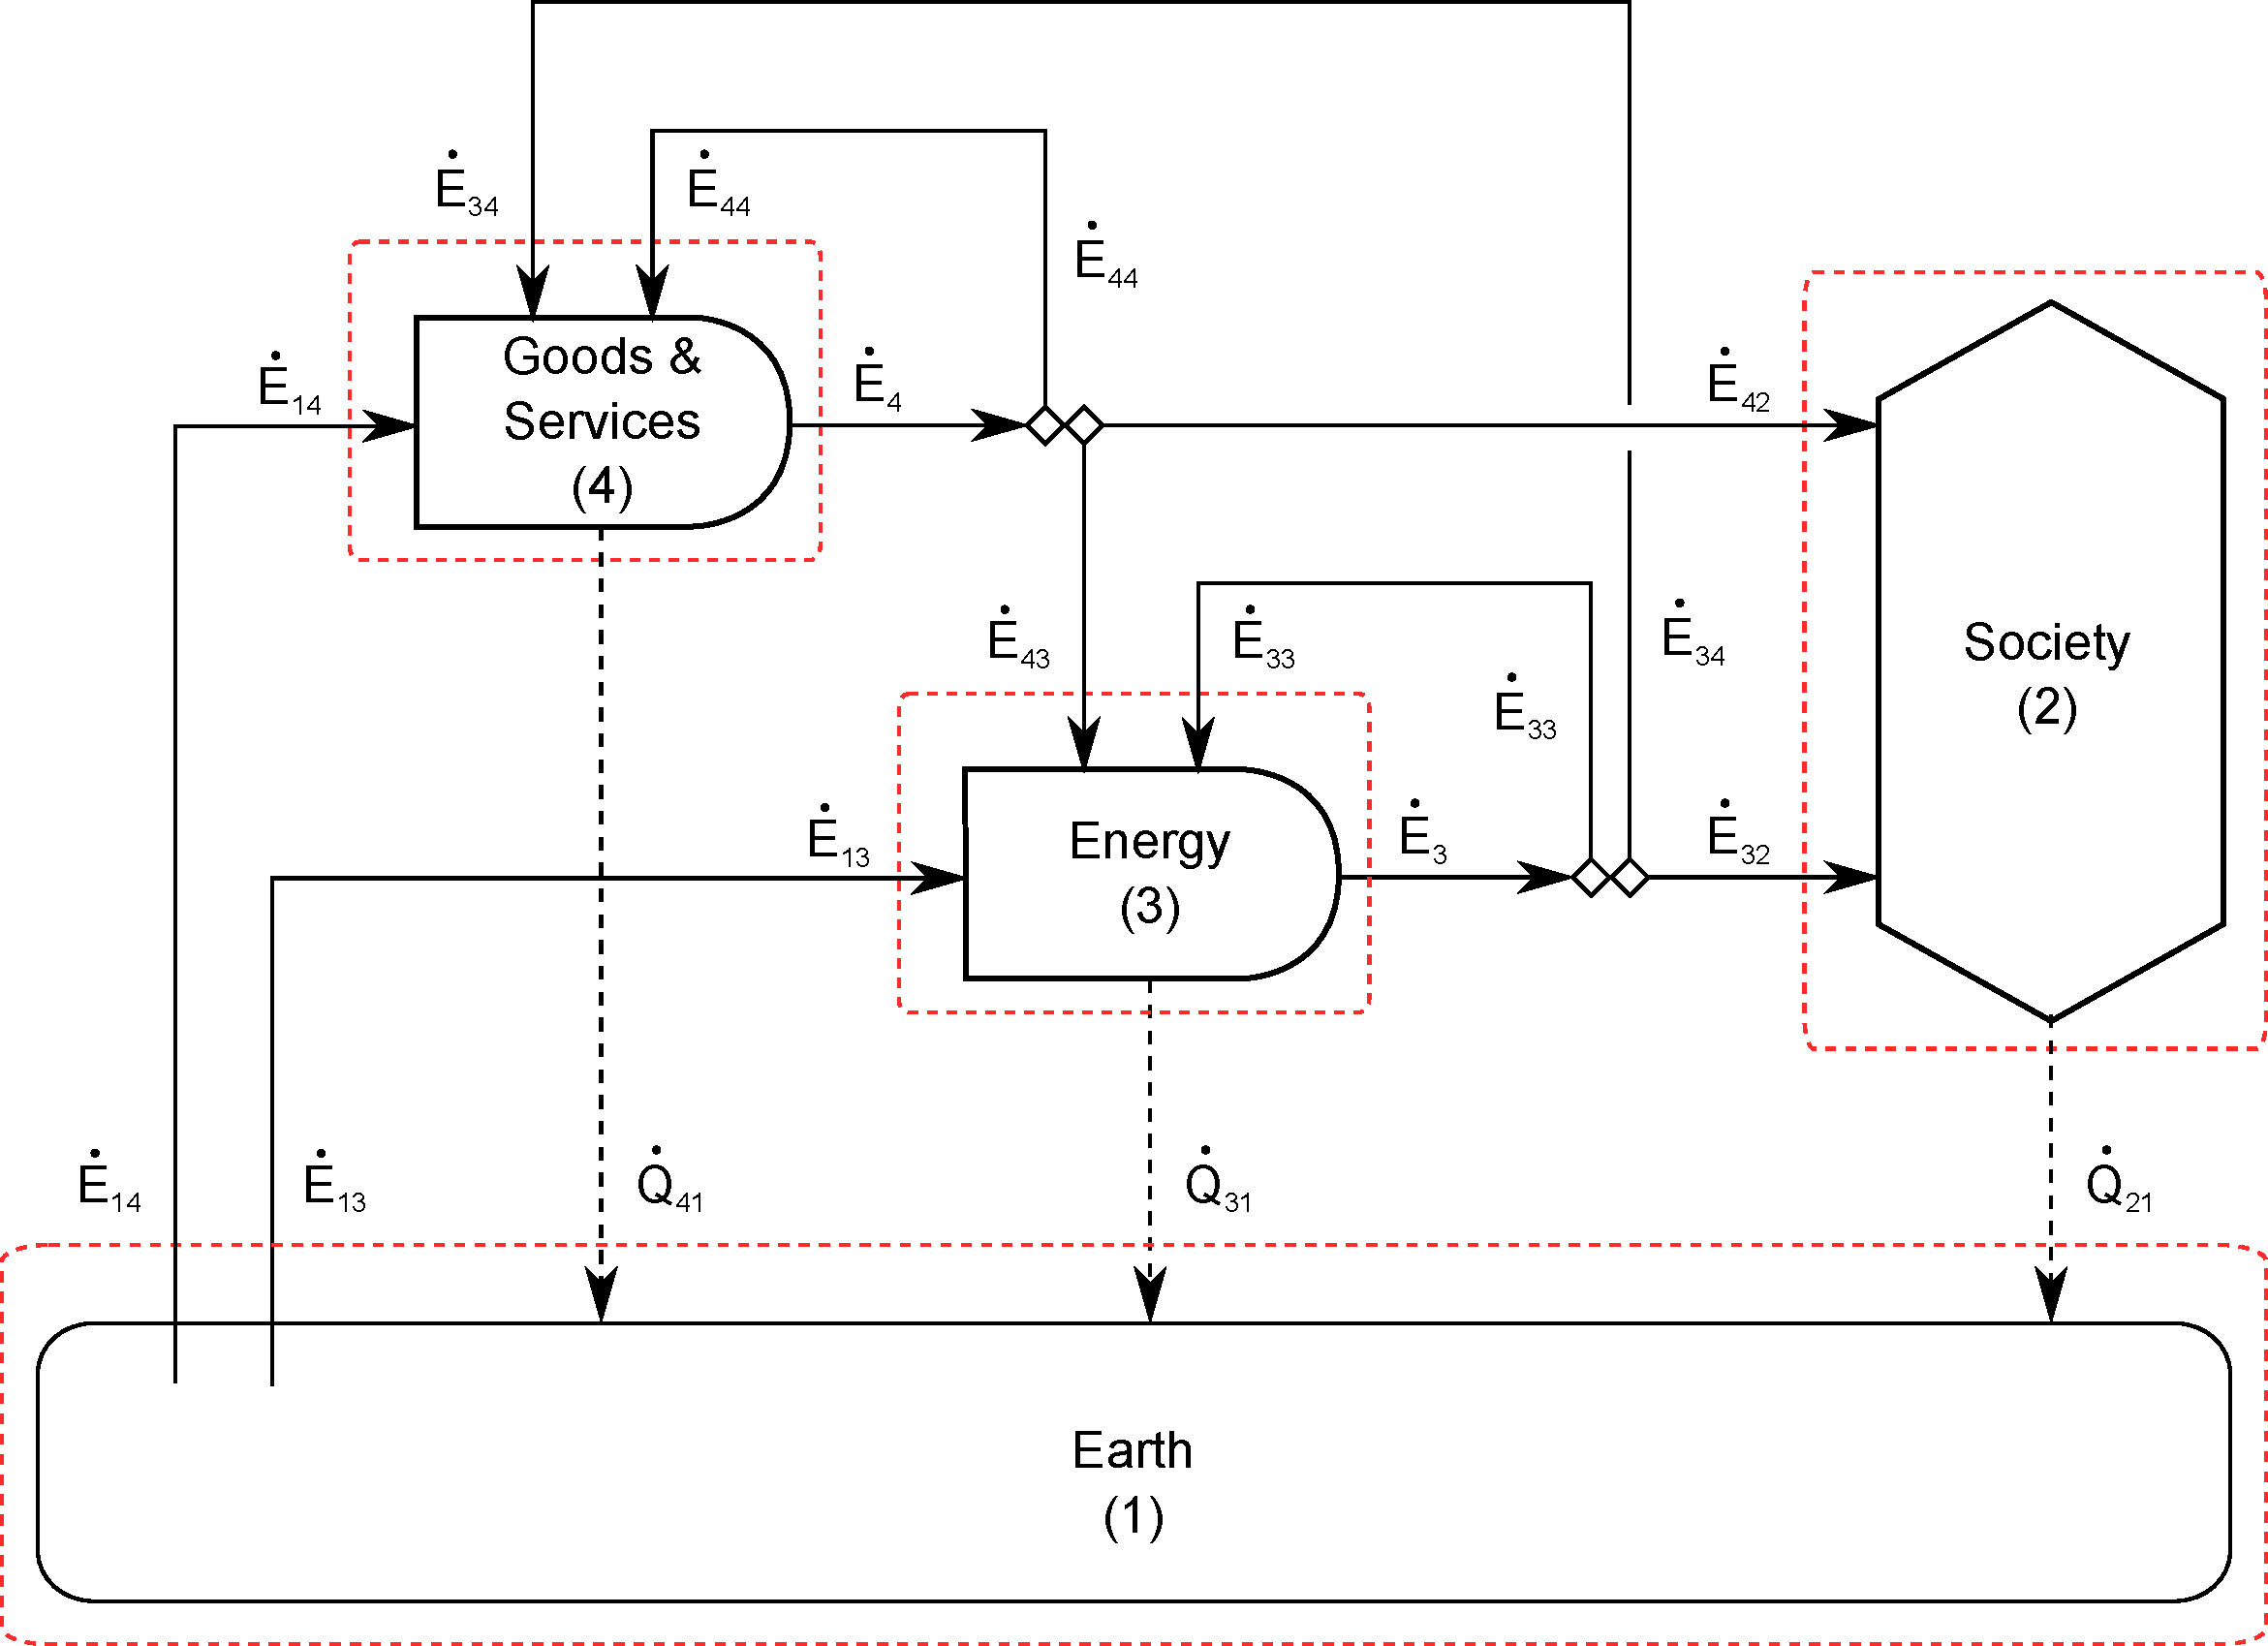
\includegraphics[width=1.0\linewidth]{Chapter_Example_C/images/I-O_three_sector_direct_energy.pdf}
\caption{Flows of direct energy ($\dot{E}$) and waste heat ($\dot{Q}$) in a two-sector economy.}
\label{fig:direct_energy_flows_2}
\end{figure}

In this economy, we assume that the purpose of the Goods and Services sector (4) is to produce goods and provide services, it provides no direct energy to society. The purpose of the Energy sector (3) is to make direct energy ($\dot{E}$) available to the economy and society in a useful form. Both direct energy ($\dot{E}$) (such as chemical potential energy in coal, oil, and electricity) and waste heat ($\dot{Q}$) are accounted by the First Law of Thermodynamics. The First Law around the Goods and Services sector (4) including, for now, the accumulation rate of direct energy in the sector $\left(\frac{\mathrm{d}E_{4}}{\mathrm{d}t}\right)$ yields

\begin{equation} \label{eq:C-CV_E_dot_4}
	\frac{\mathrm{d}E_{4}}{\mathrm{d}t} 	 =  \dot{E}_{14} + \dot{E}_{34} + \dot{E}_{44} - \dot{E}_4 - \dot{Q}_{41}.
\end{equation}

Note that we may simplify Equation \ref{eq:C-CV_E_dot_4} by realizing that $\dot{E}_{4} = \dot{E}_{4i} = 0$, because the goods and services sector is assumed to produce no flows of energy, and that $\dot{E}_{14} = 0$, since sector (4) receives no direct energy from the earth, except via the energy sector (3), hence:

\begin{equation} \label{eq:C-CV_E_dot_4_simp}
	\frac{\mathrm{d}E_{4}}{\mathrm{d}t} 	 =  \dot{E}_{34} - \dot{Q}_{41}.
\end{equation}

% [HOW DO WE WANT TO ACCOUNT FOR FOOD (i.e. ENERGY) OUTPUT FROM SECTOR (4) WHICH FLOWS INTO SECTOR (2) IN THIS FRAMEWORK? SIMILARLY, THERE ARE ENERGY FLOWS WHICH ARE USED INTERNALLY (E.G. FERTILIZERS, SO SHOULD WE HAVE $\dot{E}_{4}$ and $\dot{E}_{44}$ TERMS] 
% [ANOTHER CONCEPTUAL QUESTION IS WHETHER AN $\dot{E}_{24}$ TERM SHOULD BE INCLUDED. LABOR IS SUPPLIED FROM SOCIETY TO THE GOODS AND SERVICES SECTOR. LABOR IS A FORM OF DIRECT ENERGY, NO? --MKH]
% [FOOTNOTE ADDED TO DEAL WITH TWO COMMENTS ABOVE - MD]

%[I DECIDED TO INCLUDE THE $\dot{E_4}$ TERM IN THE ABOVE EQUATION. WE DON'T NEED AN $\dot{E}_{44}$ TERM. --MKH. I DON'T FOLLOW WHY WE DON'T NEED THE $\dot{E}_{44}$ TERM? - MD.]



The First Law of Thermodynamics around the Earth (1), Society (2), and the Energy sector (3) gives

\begin{equation} \label{eq:C-CV_E_dot_1}
	\frac{\mathrm{d}E_{1}}{\mathrm{d}t} 	 =  \dot{Q}_{21} + \dot{Q}_{31} + \dot{Q}_{41} - \dot{E}_{13} - \dot{E}_{14},
\end{equation}

\begin{equation} \label{eq:C-CV_E_dot_2}
	\frac{\mathrm{d}E_{2}}{\mathrm{d}t} 	 = \dot{E}_{32}  + \dot{E}_{42} - \dot{Q}_{21},
\end{equation}

\noindent and 

\begin{equation} \label{eq:C-CV_E_dot_3}
	\frac{\mathrm{d}E_{3}}{\mathrm{d}t} 	 = \dot{E}_{13} + \dot{E}_{33} + \dot{E}_{43} - \dot{E}_{3} - \dot{Q}_{31}.
\end{equation}

As in Examples A and B, we can set the accumulation of direct energy to zero.

\begin{equation} \label{eq:C-CV_E_dot_1_SS}
	0 =  \dot{Q}_{21} + \dot{Q}_{31} + \dot{Q}_{41} - \dot{E}_{13} - \dot{E}_{14}
\end{equation}

\begin{equation} \label{eq:C-CV_E_dot_2_SS}
	0  = \dot{E}_{32}  + \dot{E}_{42} - \dot{Q}_{21}
\end{equation}

\begin{equation} \label{eq:C-CV_E_dot_3_SS}
	0 = \dot{E}_{13} + \dot{E}_{33} + \dot{E}_{43} - \dot{E}_{3} - \dot{Q}_{31}
\end{equation}

\noindent and 

\begin{equation} \label{eq:C-CV_E_dot_4_SS}
	0 = \dot{E}_{14} + \dot{E}_{34} + \dot{E}_{44} - \dot{E}_4 - \dot{Q}_{41}
\end{equation}

%%%%%%%%%% Example C %%%%%%%%%%
\section{Total energy accounting}
%%%%%%%%%%

Again, we follow the I-O literature in assuming that total energy (i.e., the sum of direct energy and embodied energy) is conserved. Thus, we can draw a diagram similar to Figure \ref{fig:direct_energy_flows_2} for total energy flows.

\begin{figure}[h!]
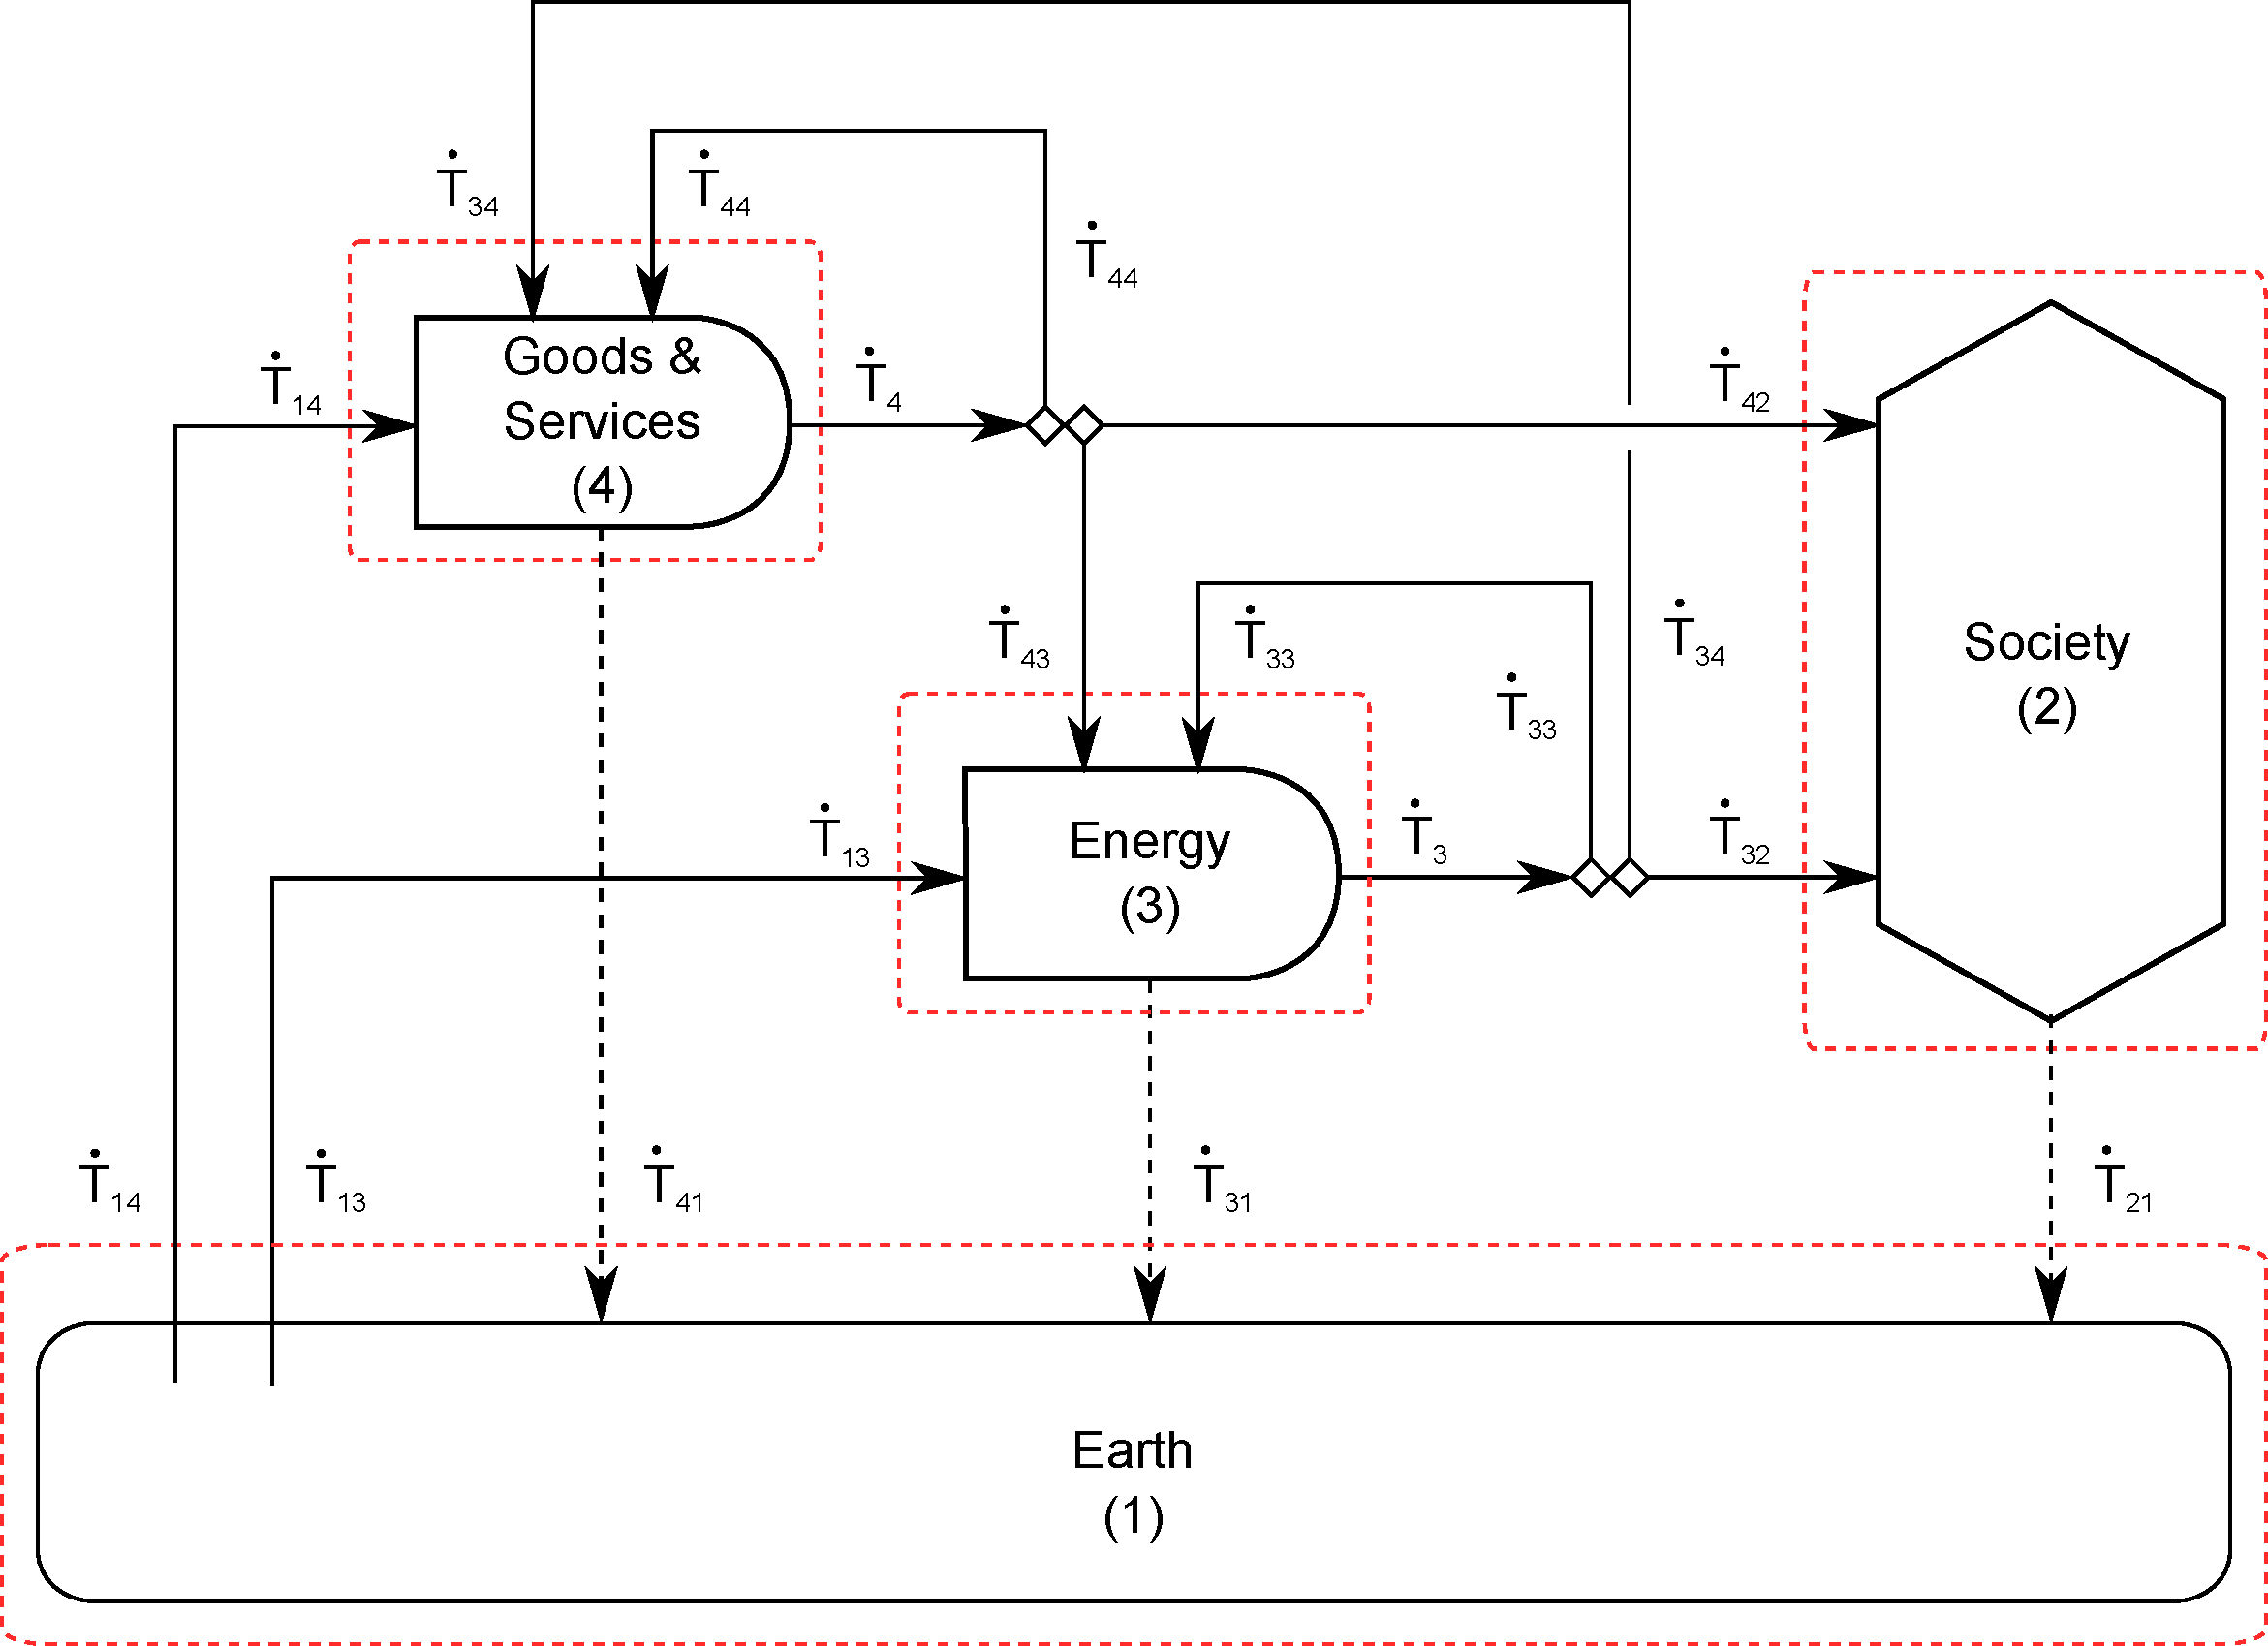
\includegraphics[width=1.0\linewidth]{Chapter_Example_C/images/I-O_three_sector_total_energy.pdf}
\caption{Flows of total energy ($\dot{T}$) in a two-sector economy.}
\label{fig:total_energy_flows_2S}
\end{figure}

Accounting for accumulation of total energy and using the assumption that total energy is conserved, we can write the following equations.

\begin{equation} \label{eq:C-CV_T_1}
	\frac{\mathrm{d}T_{1}}{\mathrm{d}t} 	 = \dot{T}_{21} + \dot{T}_{31} + \dot{T}_{41} - \dot{T}_{13} - \dot{T}_{14},
\end{equation}

\begin{equation} \label{eq:C-CV_T_2}
	\frac{\mathrm{d}T_{2}}{\mathrm{d}t} 	 = \dot{T}_{32} + \dot{T}_{42} - \dot{T}_{21},
\end{equation}

\begin{equation} \label{eq:C-CV_T_3}
	\frac{\mathrm{d}T_{3}}{\mathrm{d}t} 	 = \dot{T}_{13} + \dot{T}_{33} + \dot{T}_{43} - \dot{T}_{3} - \dot{T}_{31},
\end{equation}

\noindent and 

\begin{equation} \label{eq:C-CV_T_4}
	\frac{\mathrm{d}T_{4}}{\mathrm{d}t} 	 = \dot{T}_{14} + \dot{T}_{34} + \dot{T}_{44} - \dot{T}_{4} - \dot{T}_{41}.
\end{equation}

%%%%%%%%%% Example C %%%%%%%%%%
\section{Embodied energy accounting}
%%%%%%%%%%

Given that $\frac{\mathrm{d}E_{i}}{\mathrm{d}t} = 0$, we again note that $\frac{\mathrm{d}T_i}{\mathrm{d}t} = \frac{\mathrm{d}B_i}{\mathrm{d}t}$. Substituting $\dot{T} = \dot{E} + \dot{B}$ into the total energy accounting equations gives

\begin{equation} \label{eq:C-CV_dB_1}
	\frac{\mathrm{d}B_{1}}{\mathrm{d}t} 	 = \dot{E}_{21} + \dot{B}_{21} + \dot{E}_{31} + \dot{B}_{31} + \dot{E}_{41} + \dot{B}_{41} - \dot{E}_{13} - \dot{B}_{13} - \dot{E}_{14} - \dot{B}_{14},
\end{equation}

\begin{equation} \label{eq:C-CV_dB_2}
	\frac{\mathrm{d}B_{2}}{\mathrm{d}t} 	 = \dot{E}_{32} + \dot{B}_{32} + \dot{E}_{42} + \dot{B}_{42} - \dot{E}_{21} - \dot{B}_{21},
\end{equation}

\begin{equation} \label{eq:C-CV_dB_3}
	\frac{\mathrm{d}B_{3}}{\mathrm{d}t} 	 = \dot{E}_{13} + \dot{B}_{13} + \dot{E}_{33} + \dot{B}_{33} + \dot{E}_{43} + \dot{B}_{43} - \dot{E}_{3} - \dot{B}_{3} - \dot{E}_{31} - \dot{B}_{31},
\end{equation}

\noindent and 

\begin{equation} \label{eq:C-CV_dB_4}
	\frac{\mathrm{d}B_{4}}{\mathrm{d}t} 	 = \dot{E}_{14} + \dot{B}_{14} + \dot{E}_{34} + \dot{B}_{34} + \dot{E}_{44} + \dot{B}_{44} - \dot{E}_{4} - \dot{B}_{4} - \dot{E}_{41} - \dot{B}_{41}.
\end{equation}

Substituting the First Law of Thermodynamics (Equations \ref{eq:C-CV_E_dot_1_SS} through \ref{eq:C-CV_E_dot_4_SS}) into the total energy accounting equations (Equations \ref{eq:C-CV_dB_1} through \ref{eq:C-CV_dB_4}) gives embodied energy accounting equations for Example C.

\begin{equation} \label{eq:C-embodied_acct_1}
	\frac{\mathrm{d}B_{1}}{\mathrm{d}t} 	 = \dot{B}_{21} + \dot{B}_{31} + \dot{B}_{41} - \dot{B}_{13} - \dot{B}_{14} - \dot{Q}_{21} - \dot{Q}_{31} - \dot{Q}_{41}
\end{equation}

\begin{equation} \label{eq:C-embodied_acct_2}
	\frac{\mathrm{d}B_{2}}{\mathrm{d}t} 	 = \dot{B}_{32} + \dot{B}_{42} + \dot{Q}_{21} - \dot{B}_{21}
\end{equation}

\begin{equation} \label{eq:C-embodied_acct_3}
	\frac{\mathrm{d}B_{3}}{\mathrm{d}t} 	 = \dot{B}_{13} + \dot{B}_{33} + \dot{B}_{43} + \dot{Q}_{31} - \dot{B}_{3} - \dot{B}_{31}
\end{equation}

\begin{equation} \label{eq:C-embodied_acct_4}
	\frac{\mathrm{d}B_{4}}{\mathrm{d}t}	 = \dot{B}_{14} + \dot{B}_{34} + \dot{B}_{44} + \dot{Q}_{41} - \dot{B}_{4} - \dot{B}_{41}
\end{equation}

To verify the above derivation, we sum Equations \ref{eq:C-embodied_acct_1} through \ref{eq:C-embodied_acct_4} and use the following identities:

\begin{equation} \label{eq:C-B_sum_3_output}
	\dot{B}_3 = \dot{B}_{32} + \dot{B}_{33} + \dot{B}_{34}
\end{equation}

\noindent and

\begin{equation} \label{eq:C-B_sum_4_output}
	\dot{B}_4 = \dot{B}_{42} + \dot{B}_{43} + \dot{B}_{44};
\end{equation}

\noindent to obtain

\begin{equation} \label{eq:C-B_sums_to_zero}
	\frac{\mathrm{d}B_{1}}{\mathrm{d}t} + \frac{\mathrm{d}B_{2}}{\mathrm{d}t} + \frac{\mathrm{d}B_{3}}{\mathrm{d}t} + \frac{\mathrm{d}B_{4}}{\mathrm{d}t} = 0
\end{equation}

\noindent as expected. The total embodied energy content of the system (Earth (1), Society (2), Energy sector (3), and Goods and Services sector (4)) is constant with respect to time.


%%%%%%%%%% Example C %%%%%%%%%%
\section{Definition of embodied energy ($\dot{B}$)}\label{sec:embodied_energy}
%%%%%%%%%%

At this point we can develop a rigorous definition of embodied energy. To do so, we use the Goods and Services sector (4) from Example C. Direct energy accounting around the Goods and Services sector (Figure \ref{fig:direct_energy_flows_2}) yields

\begin{equation} \label{eq:CV_around_GS_sector_E_dot}
	\frac{\mathrm{d}E_{4}}{\mathrm{d}t} = \dot{E}_{14} + \dot{E}_{34} + \dot{E}_{44} - \dot{E}_{4} - \dot{Q}_{41},
\end{equation}

Total energy accounting around the Goods and Services sector (Figure \ref{fig:total_energy_flows_2S}) yields

\begin{equation} \label{eq:CV_around_GS_sector_T_dot}
	\frac{\mathrm{d}T_{4}}{\mathrm{d}t} = \dot{T}_{14} + \dot{T}_{34} + \dot{T}_{44} - \dot{T}_{4} + \dot{T}_{41},
\end{equation}

Solving the direct energy equation (Equation \ref{eq:CV_around_GS_sector_E_dot}) for the rate of direct energy input from the Energy sector (3) to the Goods and Services sector (4), namely $\dot{E}_{34}$, substituting into the total energy equation (Equation \ref{eq:CV_around_GS_sector_T_dot}), solving the result for $\dot{B}_{4}$, and assuming that no direct energy is wasted by the Goods and Services sector (4) to the Earth (1), i.e. $\dot{E}_{41} = 0$, yields

\begin{equation} \label{eq:embodied_output_GS}
	\dot{B}_{4} = \dot{B}_{14} + \dot{B}_{34} + \dot{B}_{44} + \dot{Q}_{41} - \frac{\mathrm{d}B_{4}}{\mathrm{d}t} - \dot{B}_{41}.
\end{equation}

Written generally, we obtain a formal definition for embodied energy output from an economic sector:

\begin{equation} \label{eq:embodied_def_1}
	\dot{B}_{j} \equiv \displaystyle\sum_{i} \dot{B}_{ij} - \frac{\mathrm{d}B_{j}}{\mathrm{d}t} - \dot{B}_{j1} + \dot{Q}_{j1}.
\end{equation}

Rearranging, we obtain

\begin{equation} \label{eq:embodied_def_2}
	\frac{\mathrm{d}B_{j}}{\mathrm{d}t} =  \displaystyle\sum_{i} \dot{B}_{ij} - \dot{B}_{j} - \dot{B}_{j1} + \dot{Q}_{j1}.
\end{equation}

In words, the rate of accumulation of embodied energy in a sector of the economy ($\frac{\mathrm{d}B_{j}}{\mathrm{d}t}$) is equal to the sum of the rates of input of embodied energy into the sector ($\displaystyle\sum_{i} \dot{B}_{ij}$) less the rate of useful output of embodied energy from the sector ($\dot{B}_{j}$) less  the rate of wasting embodied energy by the sector ($\dot{B}_{j1}$) \emph{plus} the rate of waste heat from the sector ($\dot{Q}_{j1}$). The first three terms on the right side of the equation are expected: accumulation is the difference between inflow and outflow rates. However, we see that the last term ($+\ \dot{Q}_{j1}$) in the above equations indicates that waste heat is \emph{additive} to both accumulation of embodied energy in a sector of the economy (Equation \ref{eq:embodied_def_2}) and outflow of embodied energy from a sector of the economy (Equation \ref{eq:embodied_def_1}). Furthermore, because the waste heat appears in the embodied energy output from a sector, waste heat accumulates along each step of a process such that the energy embodied in a finished product is the \emph{sum} of waste heats along a process path.


%%%%%%%%%% Example C %%%%%%%%%%
 \section{Depreciation}
%%%%%%%%%%

[SOMEWHERE WE NEED TO DISCUSS THE $\dot{S}_{i1}$ TERMS]

The terms $\dot{B}_{21}$,  $\dot{B}_{31}$, and $\dot{B}_{41}$ represent material depreciation (i.e., disposal) rates. As before, we can represent the embodied energy content of material depreciation as $\dot{B}_{i1} = \gamma_i B_i$ to obtain

\begin{equation} \label{eq:C-embodied_acct_1_depreciation}
	\frac{\mathrm{d}B_{1}}{\mathrm{d}t} 	 = \gamma_2 B_2 + \gamma_3 B_3 + \gamma_4 B_4 - \dot{B}_{13} - \dot{B}_{14} - \dot{Q}_{21} - \dot{Q}_{31} - \dot{Q}_{41}
\end{equation}

\begin{equation} \label{eq:C-embodied_acct_2_depreciation}
	\frac{\mathrm{d}B_{2}}{\mathrm{d}t} 	 = \dot{B}_{32} + \dot{B}_{42} + \dot{Q}_{21} - \gamma_2 B_2
\end{equation}

\begin{equation} \label{eq:C-embodied_acct_3_depreciation}
	\frac{\mathrm{d}B_{3}}{\mathrm{d}t} 	 = \dot{B}_{13} + \dot{B}_{33} + \dot{B}_{43} + \dot{Q}_{31} - \dot{B}_{3} - \gamma_3 B_3
\end{equation}

\begin{equation} \label{eq:C-embodied_acct_4_depreciation}
	\frac{\mathrm{d}B_{4}}{\mathrm{d}t}	 = \dot{B}_{14} + \dot{B}_{34} + \dot{B}_{44} + \dot{Q}_{41} - \dot{B}_{4} - \gamma_4 B_4
\end{equation}

%%%%%%%%%% Example C %%%%%%%%%%
%\section{Energy ratios}
%%%%%%%%%%%
%
%% [MIK: I MOVED THESE ENERGY RATIOS TO HERE FROM EARLIER, BECAUSE THEY NEED TO APPEAR AFTER WE DID THE TOTAL ENERGY ACCOUNTING FOR EXAMPLE C. YOU NEED TO REVIEW THIS SECTION IN LIGHT OF ALL OUR CHANGES. --MKH] 
%
%[THIS SECTION IS INTERESTING TO US, BUT MAY NOT BE GERMANE TO THE PAPER. IF THIS WERE TO BE A BOOK, I THINK WE SHOULD KEEP THIS SECTION IN. IF WE'RE NOW SHOOTING FOR A PAPER, WE CAN PROBABLY LEAVE THIS SECTION OUT. WE SHOULD AT LEAST REFERENCE THE LITERATURE HERE. OR, WE SHOULD MAKE USE OF THESE RATIOS. FOR EXAMPLE, IF WE WANT TO TALK ABOUT DECLINING RESOURCE QUALITY IN TERMS OF $EROI$ OR $GER$, WE SHOULD DO SO. WE SHOULD THEN SUBSTITUTE $GER$ INTO THE DERIVED EQUATIONS AND SHOW HOW A CHANGE IN $GER$ AFFECTS ENERGY FLOWS THROUGH THE ECONOMY.  --MKH]
%
%Several important energy ratios can be observed in Figure \ref{fig:direct_energy_flows_2}. [REFERENCE OTHER PAPERS FOR NOMENCLATURE? --MKH] The Gross Energy Ratio ($GER$) is defined as: 
%
%\begin{equation} \label{eq:C-GER_def}
%	GER_{\beta} \equiv \frac{\dot{E}_{3}}{\dot{E}_{33}}.
%\end{equation}
%
%\noindent The Net Energy Ratio ($NER$) is defined as [SHOULD THE NUMERATOR FOR $NER_\beta$ BE $\dot{E}_{32} + \dot{E}_{34}$? --MKH]
%
%[MIK SHOULD CHECK THE NEXT TWO EQUATIONS. ARE THEY CORRECT? --MKH]
%
%\begin{equation} \label{eq:NER_beta_def}
%	NER_{\beta} \equiv \frac{\dot{E}_{32}}{\dot{E}_{33}} = GER - 1.
%\end{equation}
%
%%[THESE DEFINITIONS ARE EQUIVALENT TO $\beta$ BOUNDARY DEFINED IN BRANDT AND DALE (2011). WE CAN DEFINE EXTERNAL ENERGY RATIO BY ACCOUNTING FOR TOTAL ENERGY FLOWS AS BELOW]
%
%[CAN WE SIMPLIFY THESE? FOR EXAMPLE, $\dot{E}_{43} = 0$, SO THE DENOMINATOR CAN BE SIMPLIFIED TO $\dot{B}_{43}$ --MKH]
%
%\begin{equation} \label{eq:C-GER_delta_def}
%	GER_{\delta} \equiv \frac{\dot{E}_{3}}{\dot{T}_{33} + \dot{T}_{43}};
%\end{equation}
%
%[THIS EQUATION DOESN'T LOOK RIGHT. IT IS SAME AS THE PREVIOUS EQUATION $GER - 1$, BUT HAS A DIFFERENT DENOMINATOR. MIK SHOULD CHECK. --MKH]
%\begin{equation} \label{eq:C-NER_delta_def}
%	NER_{\beta} \equiv \frac{\dot{E}_{32} + \dot{E}_{34}}{\dot{T}_{33} + \dot{T}_{43}} = GER - 1;
%\end{equation}
%
%We may also define a Gross External Energy Ratio (GEER) and Net External Energy Ratio (NEER), which account only for inputs from other sectors in the denominator:
%
%\begin{equation} \label{eq:C-GEER_delta_def}
%	GEER_{\delta} \equiv \frac{\dot{E}_{3}}{\dot{T}_{43}},
%\end{equation}
%
%and
%
%\begin{equation} \label{eq:C-NEER_delta_def}
%	NEER_{\beta} \equiv \frac{\dot{E}_{32}}{\dot{T}_{43}}.
%\end{equation}

%%%%%%%%%% Example C %%%%%%%%%%
\section{Final demand}
%%%%%%%%%%

Society's demand vector for total energy, $\dot{T}$, can be written as 

\begin{equation} \label{eq:demand_vector_T_dot}
	\vec{Y}_{\dot{T}} = 	\begin{Bmatrix} 	\dot{T}_{32}	\\
																\dot{T}_{42}	\\
									\end{Bmatrix}.
\end{equation}

\noindent In terms of total energy, the ultimate demand ($Y_{\dot{T}}$) is given by 

\begin{equation} \label{eq:final_demand_T_sum}
	Y_{\dot{T}} = 	\sum_{i=3}^{N} \dot{T}_{i2} = \dot{T}_{32} + \dot{B}_{42}.
\end{equation}

\noindent after realizing that $\dot{E}_{42} = 0$. 

[IS THE FOLLOWING PARAGRAPH IN THE RIGHT PLACE?]

We acknowledge that there are examples in the real economy which run counter to this model, where output from non-energy sectors are valued for their energetic content, one example being agriculture.  ``Direct'' energy inputs also flow in the opposite direction in the form of labor, which we also neglect. This will serve to introduce errors which will be small for industrial economies and larger for less industrial societies. To illustrate this we may compare the United States with India. To feed an adult requires around 2000 kcal/day $\approx$ 3 GJ/yr. To feed the whole $\sim$300 million population of the States requires around 1$\times 10^{18}$J (1 EJ) which is around 1\% of the roughly 100 EJ of primary energy supply. The US labor force currently stands at around 240 million. Given that a human can supply around 100 W of power and assuming an 8 hour work day, the US labor force will supply 70 TWh/yr $\approx$ 0.25 EJ. For India, the energy to food to feed 1.25 billion people is nearly 4 EJ which is around 15\% of the $\sim$25 EJ of primary energy consumed. Assuming that the labor force makes up 500 million people working at 12 hours per day, the energy supplied by labor is around 0.8 EJ or around 3\% of the total primary energy. As such, we can see that food energy accounts for around 1\% of primary energy in the US and around 15\% in India. Similarly, the labor inputs account for around 0.25\% in the US and around 3\% in India. The implication of including or omitting these flows is different in each case. Our assumptions introduce small errors for industrial societies where most of the world's energy is consumed.

Using $\dot{T}_{32} = \dot{E}_{32} + \dot{B}_{32}$ and rearranging Equation \ref{eq:final_demand_T_sum} gives

\begin{equation} \label{eq:rearranged_final_demand_T_sum}
	\dot{B}_{32} + \dot{B}_{42} = Y_{\dot{T}} - \dot{E}_{32}.
\end{equation}

\noindent Substituting Equation \ref{eq:rearranged_final_demand_T_sum} into Equation \ref{eq:C-embodied_acct_2_depreciation} yields

\begin{equation} \label{eq:intermediate_T_sum_dB2_dt}
	\frac{\mathrm{d}B_2}{\mathrm{d}t} = Y_{\dot{T}} - \dot{E}_{32} + \dot{Q}_{21} - \gamma_2 B_2.
\end{equation}

Substituting Equation \ref{eq:C-CV_E_dot_2_SS} into Eqaution \ref{eq:intermediate_T_sum_dB2_dt} and realizing that $\dot{E}_{42} = 0$ because direct energy is supplied to society by the energy sector only, we obtain 

\begin{equation} \label{eq:compare_demand_and_accumulation}
	\frac{\mathrm{d}B_{2}}{\mathrm{d}t} = Y_{\dot{T}} - \gamma_{2}B_{2},
\end{equation}

[IT WOULD BE GOOD TO FIND SOME VERY ROUGH DATA FOR THIS VALUE, E.G. WHAT IS THE AVERAGE LIFETIME OF MANUFACTURED GOODS - INCLUDING PACKAGING AND NON-CONSUMER GOODS. WHAT IS THE BALANCE OF NON-DURABLE VS. DURABLE GOODS? WHAT PROPORTION OF GOODS (E.G. FOOD) IS WASTED BEFORE EVER BEING CONSUMED?]

[I AGREE. HOW? --MKH]

\noindent indicating that the final demand vector for total energy ($Y_{\dot{T}}$) and the accumulation rate of energy in society $\left(\frac{\mathrm{d}B_{2}}{\mathrm{d}t}\right)$ differ by the rate of disposal from society ($\gamma_{2}B_{2}$). We note that as total embodied energy in society ($B_{2}$) becomes increasingly large, we need an ever-increasing rate of energy supplied to the society ($Y_{\dot{T}}$) to maintain positive growth $\left(\frac{\mathrm{d}B_{2}}{\mathrm{d}t}\right)$. [MAIN POINT THAT MUST BE DISCUSSED IN FURTHER DETAIL LATER, PARTICULARLY IN RELATION TO INCREASING GDP NOT NECESSARILY SIGNALING INCREASING ACCUMULATION OR GROWTH.]

%[WE NEVER USE THE FINAL PARAGRAPHS OF THIS SECTION. I PROPOSE THAT WE DELETE THEM. --MKH]
%
%A control volume around the economy gives
%
%\begin{equation} \label{eq:CV_around_economy_B_dot}
%	Y_{\dot{B}} = \sum_{j=1}^{N} \dot{E}_{1j} - \sum_{i=1}^{N} \dot{B}_{i1} - \dot{Q}_{21},
%\end{equation}
%
%[I HAVE ADDED $\dot{Q}_{21}$ TERM HERE, AS THERE IS DEFINITELY WASTE HEAT FROM CONSUMPTION OF FINAL ENERGY $Y_{\dot{B}}$ THAT IS NOT EMBODIED IN GOOD OR SERVICE, E.G. THE ELECTRICITY I USE TO COOK MY DINNER, OR WATCH TV]
%
%\noindent illustrating that final demand to society ($Y_{\dot{B}}$) can be considered the ultimate energy sink in the absence of depreciation in the economy.
%
%It is also interesting to note that 
%
%\begin{equation} \label{eq:flow_more_than_demand}
%	\sum_{i=1}^{N} \dot{T}_{i} > Y_{\dot{T}},
%\end{equation}
%
%\noindent which is a consequence of the self-demand of sectors within the economy.

%%%%%%%%%% Example C %%%%%%%%%%
\section{Flows of Value ($\dot{X}$)}
%%%%%%%%%%

The following figure shows value flows ($\dot{X}$) in the two-sector economy.

\begin{figure}[h!]
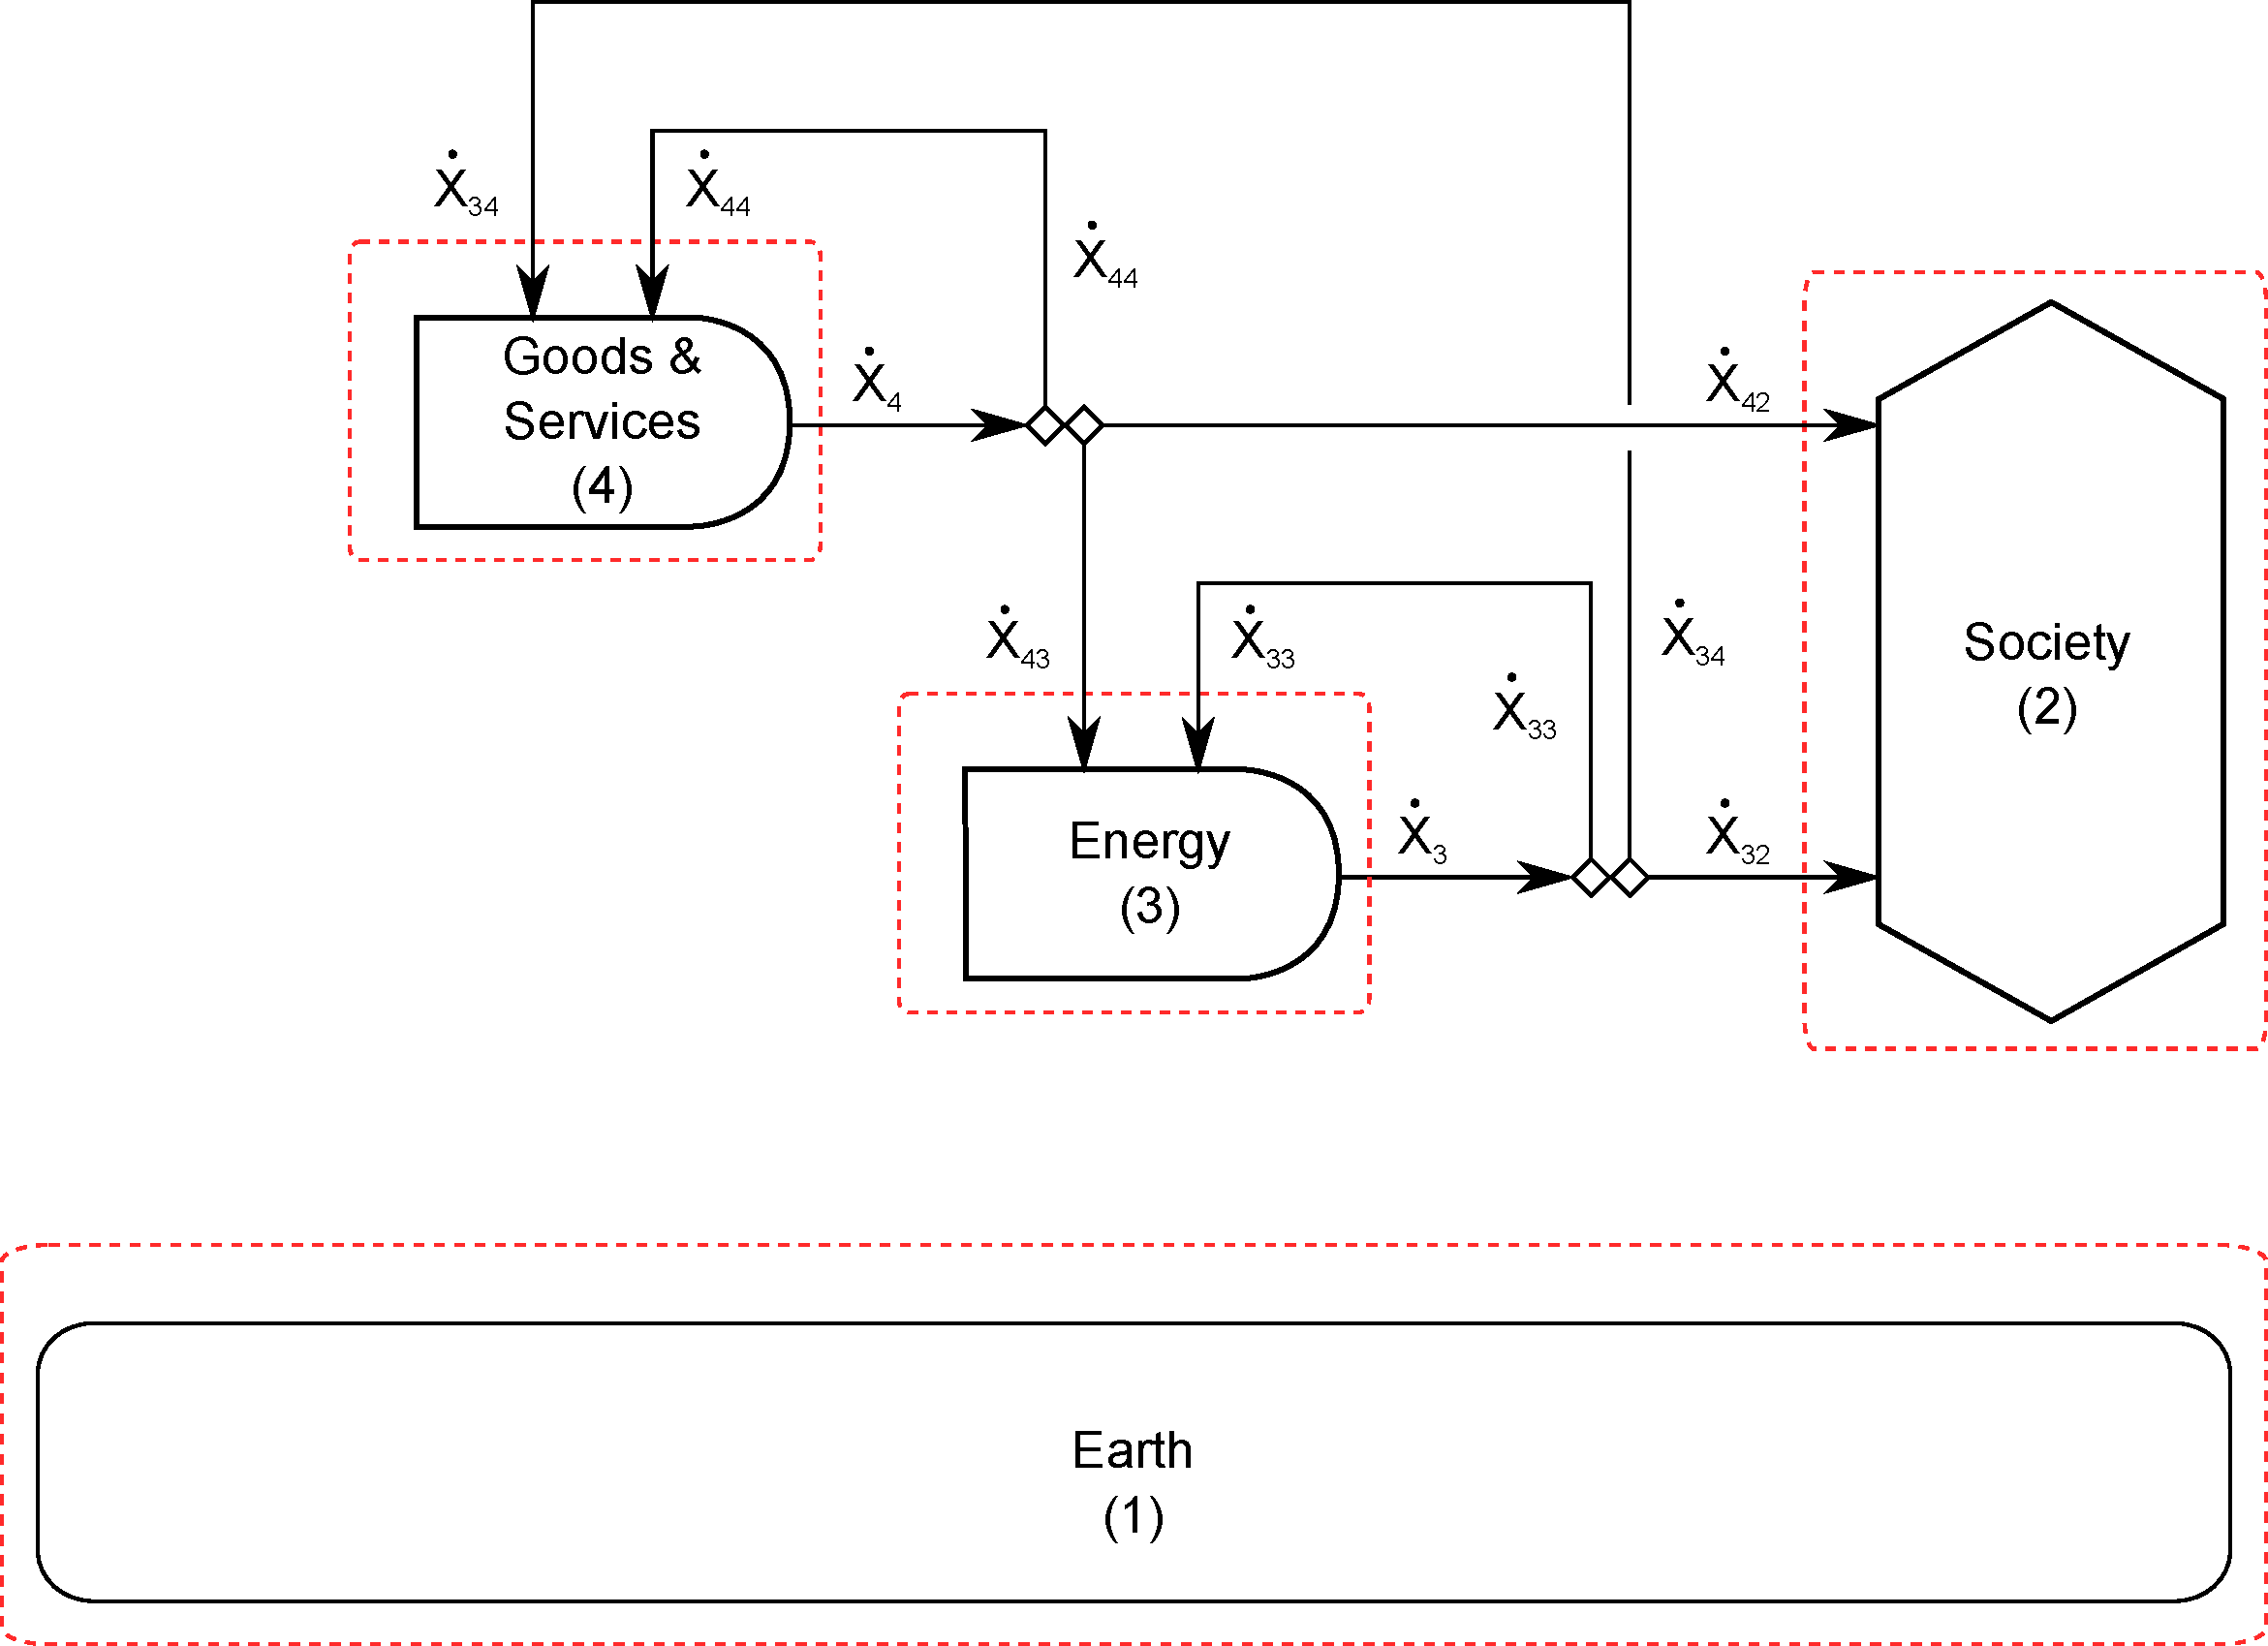
\includegraphics[width=1.0\linewidth]{Chapter_Example_C/images/I-O_three_sector_value.pdf}
\caption{Flows of economic value ($\dot{X}$) in a two-sector economy.}
\label{fig:economic_value_flows_2}
\end{figure}

Realizing that the valuable output from energy sectors is direct energy, $\dot{X}_{3} = \dot{E}_{3}$ and $\dot{X}_{3j} = \dot{E}_{3j}$. Thus, outputs from energy sectors are given in energy units (joules or BTUs). 

%With reference to Equations \ref{eq:GER_def_ch_5} and \ref{eq:NER_def_ch_5}, we can express the Gross Energy Ratio ($GER$) and Net Energy Ratio ($NER$) as
%
%\begin{equation} \label{eq:GER_in_terms_of_a_2}
%	GER_{\gamma} = \frac{\dot{E}_{3}}{\dot{E}_{33}} = \frac{\dot{X}_{3}}{\dot{X}_{33}} = \frac{1}{a_{33}},
%\end{equation}
%
%\noindent and
%
%\begin{equation} \label{eq:NER_in_terms_of_a_2}
%	NER = GER - 1 = \frac{1}{a_{33}} - 1.
%\end{equation}
%
%[DO WE NEED THESE NEXT TWO EQUATIONS? DO WE USE THEM ANYWHERE? THEY MIGHT BE HELPFUL FOR A GDP DISCUSSION, BUT WE HAVEN'T INCLUDED THAT DISCUSSION YET. --MKH]

Written in terms of value flows, the ultimate demand vector ($\vec{Y}$) is given by

\begin{equation} \label{eq:demand_vector_B_dot}
	\vec{Y}_{\dot{X}} = 	\begin{Bmatrix} 	\dot{X}_{32}	\\
																\dot{X}_{42}	\\
									\end{Bmatrix},
\end{equation}

\noindent and the total value demand from society ($Y$) is 

\begin{equation} \label{eq:total_value_demand}
	Y_{\dot{X}} = \sum_{i=1}^{N} \dot{X}_{i2} = \dot{X}_{32} + \dot{X}_{42}.
	\end{equation}


%%%%%%%%%% Example C %%%%%%%%%%
\section{Matrix Formulation}
%%%%%%%%%%

We can use Equations \ref{eq:epsilon_output_def} through \ref{eq:epsilon_equiv_1} to rewrite Equations \ref{eq:C-CV_B_1_depreciation} and \ref{eq:C-CV_B_2_depreciation} as

\begin{equation} \label{eq:CV_B_3_with_eps}
	\dot{X}_{33}\varepsilon_{3} + \dot{X}_{43}\varepsilon_{4} + \dot{E}_{13} - \frac{\mathrm{d}B_{3}}{\mathrm{d}t} - \gamma_{3}B_{3} = \dot{X}_{3}\varepsilon_{3}
\end{equation}

\noindent and 

\begin{equation} \label{eq:CV_B_4_with_eps}
	\dot{X}_{34}\varepsilon_{3} + \dot{X}_{44}\varepsilon_{4} + \dot{E}_{14} - \frac{\mathrm{d}B_{4}}{\mathrm{d}t} - \gamma_{4}B_{4} = \dot{X}_{4}\varepsilon_{4}.
\end{equation}

We can rewrite Equations \ref{eq:CV_B_3_with_eps} and \ref{eq:CV_B_4_with_eps} in matrix notation with the following definitions:

\begin{equation} \label{eq:eps_vec_def}
	\vec{\varepsilon} =		\begin{Bmatrix} 	\varepsilon_{3}	\\
																\varepsilon_{4}	\\
									\end{Bmatrix},
\end{equation}

\begin{equation} \label{eq:E_vec_def}
	\vec{E} =		\begin{Bmatrix} 	\dot{E}_{13}	\\
													\dot{E}_{14}\\
						\end{Bmatrix},
\end{equation}

\begin{equation} \label{eq:dBdt_vec_def}
	\frac{\mathrm{d}\vec{B}}{\mathrm{d}t} =	\begin{Bmatrix}	\frac{\mathrm{d}B_{3}}{\mathrm{d}t}	\\
																									\frac{\mathrm{d}B_{4}}{\mathrm{d}t}\\
																		\end{Bmatrix},
\end{equation}

\begin{equation} \label{eq:B_vec_def}
	\vec{B} =			\begin{Bmatrix}	B_{3}\\
														B_{4}\\
							\end{Bmatrix},
\end{equation}

\begin{equation} \label{eq:A_matrix_def}
	\vec{A} =	\begin{bmatrix} 	a_{33} & a_{34}	\\
												a_{43} & a_{44}	\\
					\end{bmatrix},
\end{equation}

\begin{equation} \label{eq:X_t_matrix_def}
	\vec{X}_{t} =		\begin{bmatrix} 	\dot{X}_{33}		&	\dot{X}_{34}	\\
														\dot{X}_{43}		&	\dot{X}_{44}\\
							\end{bmatrix},
\end{equation}

\begin{equation} \label{eq:X_hat_matrix_def}
	\hat{\vec{X}} = \delta_{ij}\dot{X}_{j} = \begin{bmatrix} 	\dot{X}_{33}		&	0					\\
																								0					&	\dot{X}_{44}	\\
																							\end{bmatrix},
\end{equation}

\begin{equation} \label{eq:B_hat_matrix_def}
	\hat{\vec{\gamma}} = \delta_{ij}\gamma_{j},
\end{equation}

[CAN WE MAKE THIS EQUATION EXPLICIT]

\noindent and

\begin{equation}\label{eq:k_delta}
	\delta_{ij} = \begin{cases}	1 	& 	\text{if  } i = j		\\
												0	&	\text{if  } i \neq j	\\
						\end{cases},
\end{equation}

\noindent such that:

\begin{equation} \label{eq:matrix_leontief}
	\vec{X}_{t}^{\mathrm{T}}\vec{\varepsilon} + \vec{E} - \left(\frac{\mathrm{d}\vec{B}}{\mathrm{d}t} + \hat{\vec{\gamma}}\vec{B}\right) = \hat{\vec{X}}\vec{\varepsilon}.
\end{equation}

Additional relationships that will be helpful later include (derived in Appendix):

\begin{equation} \label{eq:Xhat_X_and_A}
	\hat{\vec{X}}^{-1}\vec{X}_{t} = \vec{A}^{\mathrm{T}},
\end{equation}

\begin{equation} \label{eq:Xdifference1}
	\vec{X}_{t}^{\mathrm{T}} - \hat{\vec{X}} = \hat{\vec{X}}(\vec{A}^{\mathrm{T}} - \vec{I}),
\end{equation}

\begin{equation} \label{eq:Xdifference2}
	\hat{\vec{X}} - \vec{X}_{t}^{\mathrm{T}} = \hat{\vec{X}}(\vec{I} - \vec{A}^{\mathrm{T}}),
\end{equation}

\noindent and

\begin{equation} \label{eq:Xdifference2_inverse}
	\left(\hat{\vec{X}} - \vec{X}_{t}^{\mathrm{T}}\right)^{-1} = (\vec{I} - \vec{A}^{\mathrm{T}})^{-1}\hat{\vec{X}}^{-1}.
\end{equation}


%%%%%%%%%% Example C %%%%%%%%%%
\section{Estimating $\vec{\varepsilon}$ and $\frac{\mathrm{d}\vec{B}}{\mathrm{d}t}$}
%%%%%%%%%%

With Equation \ref{eq:matrix_leontief}, we can solve for either the energy accumulation vector ($\vec{\frac{\mathrm{d}B}{\mathrm{d}t}}$) or the energy intensity vector ($\vec{\varepsilon}$), but not both. 

Solving for the accumulation vector gives

\begin{equation} \label{eq:dB_dt_leontief}
	\frac{\mathrm{d}\vec{B}}{\mathrm{d}t} = (\vec{X}_{t}^{\mathrm{T}} - \hat{\vec{X}})\vec{\varepsilon} + \vec{E} - \hat{\vec{\gamma}}\vec{B}.
\end{equation}

\noindent Finally, we can substutute Equation \ref{eq:Xdifference1} which gives

\begin{equation} \label{eq:dB_dt_leontief_with_A}
	\frac{\mathrm{d}\vec{B}}{\mathrm{d}t} = \hat{\vec{X}} (\vec{A}^{\mathrm{T}} - \vec{I}) \vec{\varepsilon} + \vec{E} - \hat{\vec{\gamma}}\vec{B},
\end{equation}

\noindent which allows estimation of the embodied energy accumulation in economic sectors $\left(\frac{\mathrm{d}\vec{B}}{\mathrm{d}t}\right)$ knowing only sector outputs ($\hat{\vec{X}}$), sector input-output ratios ($\vec{A}$), sector energy intensities ($\vec{\varepsilon}$), energy input to the economy ($\vec{E}$), and sector physical depreciation rates ($\hat{\vec{\gamma}}\vec{b}$). In theory, the transaction matrix ($\vec{X}_{t}$) is not required if the input-ouput ratios ($\vec{A}$) are known, though in reality, knowledge of input-output ratios would be derived from the transaction matrix $\vec{X}_{t}$ .

Solving for the energy intensity vector gives

\begin{equation} \label{eq:epsilon_leontief}
	\vec{\varepsilon} = (\hat{\vec{X}} - \vec{X}_{t}^{\mathrm{T}})^{-1}\left[\vec{E} - \left(\frac{\mathrm{d}\vec{B}}{\mathrm{d}t} + \hat{\vec{\gamma}}\vec{B}\right)\right].
\end{equation}

\noindent Substituting Equation \ref{eq:Xdifference2_inverse} gives

\begin{equation} \label{eq:epsilon_leontief_with_A}
	\vec{\varepsilon} = (\vec{I} - \vec{A}^{\mathrm{T}})^{-1}\hat{\vec{X}}^{-1}\left[\vec{E} - \left(\frac{\mathrm{d}\vec{B}}{\mathrm{d}t} + \hat{\vec{\gamma}}\vec{B}\right)\right],
\end{equation}

\noindent which allows estimation of the energy intensity of economic sectors ($\vec{\varepsilon}$) knowing only sector input-output ratios ($\vec{A}$), sector outputs ($\hat{\vec{X}}$), energy input to the economy ($\vec{E}$), sector embodied energy accumulation rates $\left(\frac{\mathrm{d}\vec{B}}{\mathrm{d}t}\right)$, and sector physical depreciation rates ($\hat{\vec{\gamma}}\vec{B}$).

Comparison of Equations \ref{eq:eps1_ss_IO} and \ref{eq:epsilon_leontief_with_A} shows the similarities between the single-sector algebraic formulation and the multi-sector matrix formulation of the I-O analysis method. This newly developed multi-sector matrix formulation can be extended to any desired level of economic and energy sector disaggregation as shown by Bullard (1975, 1978) and others.

************************** MATT ENDED HERE *************************


\bibliography{EROI_review_v2}
\bibliographystyle{unsrt}


% Always give a unique label
% and use \ref{<label>} for cross-references
% and \cite{<label>} for bibliographic references
% use \sectionmark{}
% to alter or adjust the section heading in the running head
%% Instead of simply listing headings of different levels we recommend to let every heading be followed by at least a short passage of text. Furtheron please use the \LaTeX\ automatism for all your cross-references and citations.

%% Please note that the first line of text that follows a heading is not indented, whereas the first lines of all subsequent paragraphs are.

%% Use the standard \verb|equation| environment to typeset your equations, e.g.
%
%% \begin{equation}
%% a \times b = c\;,
%% \end{equation}
%
%% however, for multiline equations we recommend to use the \verb|eqnarray|
%% environment\footnote{In physics texts please activate the class option \texttt{vecphys} to depict your vectors in \textbf{\itshape boldface-italic} type - as is customary for a wide range of physical subjects.}.
%% \begin{eqnarray}
%% a \times b = c \nonumber\\
%% \vec{a} \cdot \vec{b}=\vec{c}
%% \label{eq:01}
%% \end{eqnarray}

%% \subsection{Subsection Heading}
%% \label{subsec:2}
%% Instead of simply listing headings of different levels we recommend to let every heading be followed by at least a short passage of text. Furtheron please use the \LaTeX\ automatism for all your cross-references\index{cross-references} and citations\index{citations} as has already been described in Sect.~\ref{sec:2}.

%% \begin{quotation}
%% Please do not use quotation marks when quoting texts! Simply use the \verb|quotation| environment -- it will automatically render Springer's preferred layout.
%% \end{quotation}


%% \subsubsection{Subsubsection Heading}
%% Instead of simply listing headings of different levels we recommend to let every heading be followed by at least a short passage of text. Furtheron please use the \LaTeX\ automatism for all your cross-references and citations as has already been described in Sect.~\ref{subsec:2}, see also Fig.~\ref{fig:1}\footnote{If you copy text passages, figures, or tables from other works, you must obtain \textit{permission} from the copyright holder (usually the original publisher). Please enclose the signed permission with the manucript. The sources\index{permission to print} must be acknowledged either in the captions, as footnotes or in a separate section of the book.}

%% Please note that the first line of text that follows a heading is not indented, whereas the first lines of all subsequent paragraphs are.

% For figures use
%
%% \begin{figure}[b]
%% \sidecaption
% Use the relevant command for your figure-insertion program
% to insert the figure file.
% For example, with the option graphics use
%% \includegraphics[scale=.65]{figure}
%
% If not, use
%\picplace{5cm}{2cm} % Give the correct figure height and width in cm
%
%% \caption{If the width of the figure is less than 7.8 cm use the \texttt{sidecapion} command to flush the caption on the left side of the page. If the figure is positioned at the top of the page, align the sidecaption with the top of the figure -- to achieve this you simply need to use the optional argument \texttt{[t]} with the \texttt{sidecaption} command}
%% \label{fig:1}       % Give a unique label
%% \end{figure}


%% \paragraph{Paragraph Heading} %
%% Instead of simply listing headings of different levels we recommend to let every heading be followed by at least a short passage of text. Furtheron please use the \LaTeX\ automatism for all your cross-references and citations as has already been described in Sect.~\ref{sec:2}.

%% Please note that the first line of text that follows a heading is not indented, whereas the first lines of all subsequent paragraphs are.

%% For typesetting numbered lists we recommend to use the \verb|enumerate| environment -- it will automatically render Springer's preferred layout.

%% \begin{enumerate}
%% \item{Livelihood and survival mobility are oftentimes coutcomes of uneven socioeconomic development.}
%% \begin{enumerate}
%% \item{Livelihood and survival mobility are oftentimes coutcomes of uneven socioeconomic development.}
%% \item{Livelihood and survival mobility are oftentimes coutcomes of uneven socioeconomic development.}
%% \end{enumerate}
%% \item{Livelihood and survival mobility are oftentimes coutcomes of uneven socioeconomic development.}
%% \end{enumerate}


%% \subparagraph{Subparagraph Heading} In order to avoid simply listing headings of different levels we recommend to let every heading be followed by at least a short passage of text. Use the \LaTeX\ automatism for all your cross-references and citations as has already been described in Sect.~\ref{sec:2}, see also Fig.~\ref{fig:2}.

%% Please note that the first line of text that follows a heading is not indented, whereas the first lines of all subsequent paragraphs are.

%% For unnumbered list we recommend to use the \verb|itemize| environment -- it will automatically render Springer's preferred layout.

%% \begin{itemize}
%% \item{Livelihood and survival mobility are oftentimes coutcomes of uneven socioeconomic development, cf. Table~\ref{tab:1}.}
%% \begin{itemize}
%% \item{Livelihood and survival mobility are oftentimes coutcomes of uneven socioeconomic development.}
%% \item{Livelihood and survival mobility are oftentimes coutcomes of uneven socioeconomic development.}
%% \end{itemize}
%% \item{Livelihood and survival mobility are oftentimes coutcomes of uneven socioeconomic development.}
%% \end{itemize}

%% \begin{figure}[t]
%% \sidecaption[t]
% Use the relevant command for your figure-insertion program
% to insert the figure file.
% For example, with the option graphics use
%% \includegraphics[scale=.65]{figure}
%
% If not, use
%\picplace{5cm}{2cm} % Give the correct figure height and width in cm
%
%% \caption{Please write your figure caption here}
%% \label{fig:2}       % Give a unique label
%% \end{figure}

%% \runinhead{Run-in Heading Boldface Version} Use the \LaTeX\ automatism for all your cross-references and citations as has already been described in Sect.~\ref{sec:2}.

%% \subruninhead{Run-in Heading Italic Version} Use the \LaTeX\ automatism for all your cross-refer\-ences and citations as has already been described in Sect.~\ref{sec:2}\index{paragraph}.
% Use the \index{} command to code your index words
%
% For tables use
%
%% \begin{table}
%% \caption{Please write your table caption here}
%% \label{tab:1}       % Give a unique label
%
% For LaTeX tables use
%
%% \begin{tabular}{p{2cm}p{2.4cm}p{2cm}p{4.9cm}}
%% \hline\noalign{\smallskip}
%% Classes & Subclass & Length & Action Mechanism  \\
%% \noalign{\smallskip}\svhline\noalign{\smallskip}
%% Translation & mRNA$^a$  & 22 (19--25) & Translation repression, mRNA cleavage\\
%% Translation & mRNA cleavage & 21 & mRNA cleavage\\
%% Translation & mRNA  & 21--22 & mRNA cleavage\\
%%Translation & mRNA  & 24--26 & Histone and DNA Modification\\
%%\noalign{\smallskip}\hline\noalign{\smallskip}
%%\end{tabular}
%%$^a$ Table foot note (with superscript)
%%\end{table}
%
%% \section{Section Heading}
%%\label{sec:3}
% Always give a unique label
% and use \ref{<label>} for cross-references
% and \cite{<label>} for bibliographic references
% use \sectionmark{}
% to alter or adjust the section heading in the running head
%% Instead of simply listing headings of different levels we recommend to let every heading be followed by at least a short passage of text. Furtheron please use the \LaTeX\ automatism for all your cross-references and citations as has already been described in Sect.~\ref{sec:2}.

%% Please note that the first line of text that follows a heading is not indented, whereas the first lines of all subsequent paragraphs are.

%%If you want to list definitions or the like we recommend to use the Springer-enhanced \verb|description| environment -- it will automatically render Springer's preferred layout.

%%\begin{description}[Type 1]
%%\item[Type 1]{That addresses central themes pertainng to migration, health, and disease. In Sect.~\ref{sec:1}, Wilson discusses the role of human migration in infectious disease distributions and patterns.}
%%\item[Type 2]{That addresses central themes pertainng to migration, health, and disease. In Sect.~\ref{subsec:2}, Wilson discusses the role of human migration in infectious disease distributions and patterns.}
%%\end{description}

%%\subsection{Subsection Heading} %
%% In order to avoid simply listing headings of different levels we recommend to let every heading be followed by at least a short passage of text. Use the \LaTeX\ automatism for all your cross-references and citations citations as has already been described in Sect.~\ref{sec:2}.

%% Please note that the first line of text that follows a heading is not indented, whereas the first lines of all subsequent paragraphs are.

%% \begin{svgraybox}
%% If you want to emphasize complete paragraphs of texts we recommend to use the newly defined Springer class option \verb|graybox| and the newly defined environment \verb|svgraybox|. This will produce a 15 percent screened box 'behind' your text.

%% If you want to emphasize complete paragraphs of texts we recommend to use the newly defined Springer class option and environment \verb|svgraybox|. This will produce a 15 percent screened box 'behind' your text.
%% \end{svgraybox}


%% \subsubsection{Subsubsection Heading}
%%Instead of simply listing headings of different levels we recommend to let every heading be followed by at least a short passage of text. Furtheron please use the \LaTeX\ automatism for all your cross-references and citations as has already been described in Sect.~\ref{sec:2}.

%% Please note that the first line of text that follows a heading is not indented, whereas the first lines of all subsequent paragraphs are.

%% \begin{theorem}
%% Theorem text goes here.
%% \end{theorem}
%
% or
%
%% \begin{definition}
%% Definition text goes here.
%% \end{definition}

%% \begin{proof}
%\smartqed
%% Proof text goes here.
%% \qed
%% \end{proof}

%%\paragraph{Paragraph Heading} %
%% Instead of simply listing headings of different levels we recommend to let every heading be followed by at least a short passage of text. Furtheron please use the \LaTeX\ automatism for all your cross-references and citations as has already been described in Sect.~\ref{sec:2}.

%% Note that the first line of text that follows a heading is not indented, whereas the first lines of all subsequent paragraphs are.
%
% For built-in environments use
%
%%\begin{theorem}
%%Theorem text goes here.
%%\end{theorem}
%
%%\begin{definition}
%%Definition text goes here.
%%\end{definition}
%
%%\begin{proof}
%%\smartqed
%% Proof text goes here.
%%\qed
%%\end{proof}
%
%% \begin{acknowledgement}
%% If you want to include acknowledgments of assistance and the like at the end of an individual chapter please use the \verb|acknowledgement| environment -- it will automatically render Springer's preferred layout.
%% \end{acknowledgement}
%
%% \section*{Appendix}
%% \addcontentsline{toc}{section}{Appendix}
%
%% When placed at the end of a chapter or contribution (as opposed to at the end of the book), the numbering of tables, figures, and equations in the appendix section continues on from that in the main text. Hence please \textit{do not} use the \verb|appendix| command when writing an appendix at the end of your chapter or contribution. If there is only one the appendix is designated ``Appendix'', or ``Appendix 1'', or ``Appendix 2'', etc. if there is more than one.

%% \begin{equation}
%% a \times b = c
%% \end{equation}
% Problems or Exercises should be sorted chapterwise
%% \section*{Problems}
%% \addcontentsline{toc}{section}{Problems}
%
% Use the following environment.
% Don't forget to label each problem;
% the label is needed for the solutions' environment
%% \begin{prob}
%% \label{prob1}
%% A given problem or Excercise is described here. The
%% problem is described here. The problem is described here.
%% \end{prob}

%% \begin{prob}
%% \label{prob2}
%% \textbf{Problem Heading}\\
%% (a) The first part of the problem is described here.\\
%% (b) The second part of the problem is described here.
%% \end{prob}


 

%%%%%%%%%%%%%%%%%%%%% chapter.tex %%%%%%%%%%%%%%%%%%%%%%%%%%%%%%%%%
%
% sample chapter
%
% Use this file as a template for your own input.
%
%%%%%%%%%%%%%%%%%%%%%%%% Springer-Verlag %%%%%%%%%%%%%%%%%%%%%%%%%%
%\motto{Use the template \emph{chapter.tex} to style the various elements of your chapter content.}
\chapter{Example D: two sector economy with durable and non-durable demand}
\chaptermark{Durable and non-durable}
\label{chap:two_sector_durable} % Always give a unique label
% use \chaptermark{}
% to alter or adjust the chapter heading in the running head

\abstract*{[NEED TO ADD ABSTRACT HERE]}

%% \abstract{Each chapter should be preceded by an abstract (10--15 lines long) that summarizes the content. The abstract will appear \textit{online} at \url{www.SpringerLink.com} and be available with unrestricted access. This allows unregistered users to read the abstract as a teaser for the complete chapter. As a general rule the abstracts will not appear in the printed version of your book unless it is the style of your particular book or that of the series to which your book belongs.\newline\indent
%% Please use the 'starred' version of the new Springer \texttt{abstract} command for typesetting the text of the online abstracts (cf. source file of this chapter template \texttt{abstract}) and include them with the source files of your manuscript. Use the plain \texttt{abstract} command if the abstract is also to appear in the printed version of the book.}

%% Use the template \emph{chapter.tex} together with the Springer document class SVMono (monograph-type books) or SVMult (edited books) to style the various elements of your chapter content in the Springer layout.


[INSERT QUOTE FROM G-R]

We now extend the two-sector economy from Example C by distinguishing between flows from sector $i$ into sector $j$ which are being processed---such as the tailor's cloth and thread, to use Georgescu-Roegen's example---and are destined to leave in the products of that sector, $\dot{T}_{j}$ (except for some proportion of wastage) and flows which are doing the processing---the tailor's needle and labor. The processed flows we term \emph{resource} flows, $\dot{R}_{ij}$ and may comprise either direct energy or energy embodied in goods or services. We assume that these do not accumulate within a sector, such that $\frac{\textrm{d}R}{\textrm{dt}} = 0$.

\begin{figure}[h!]
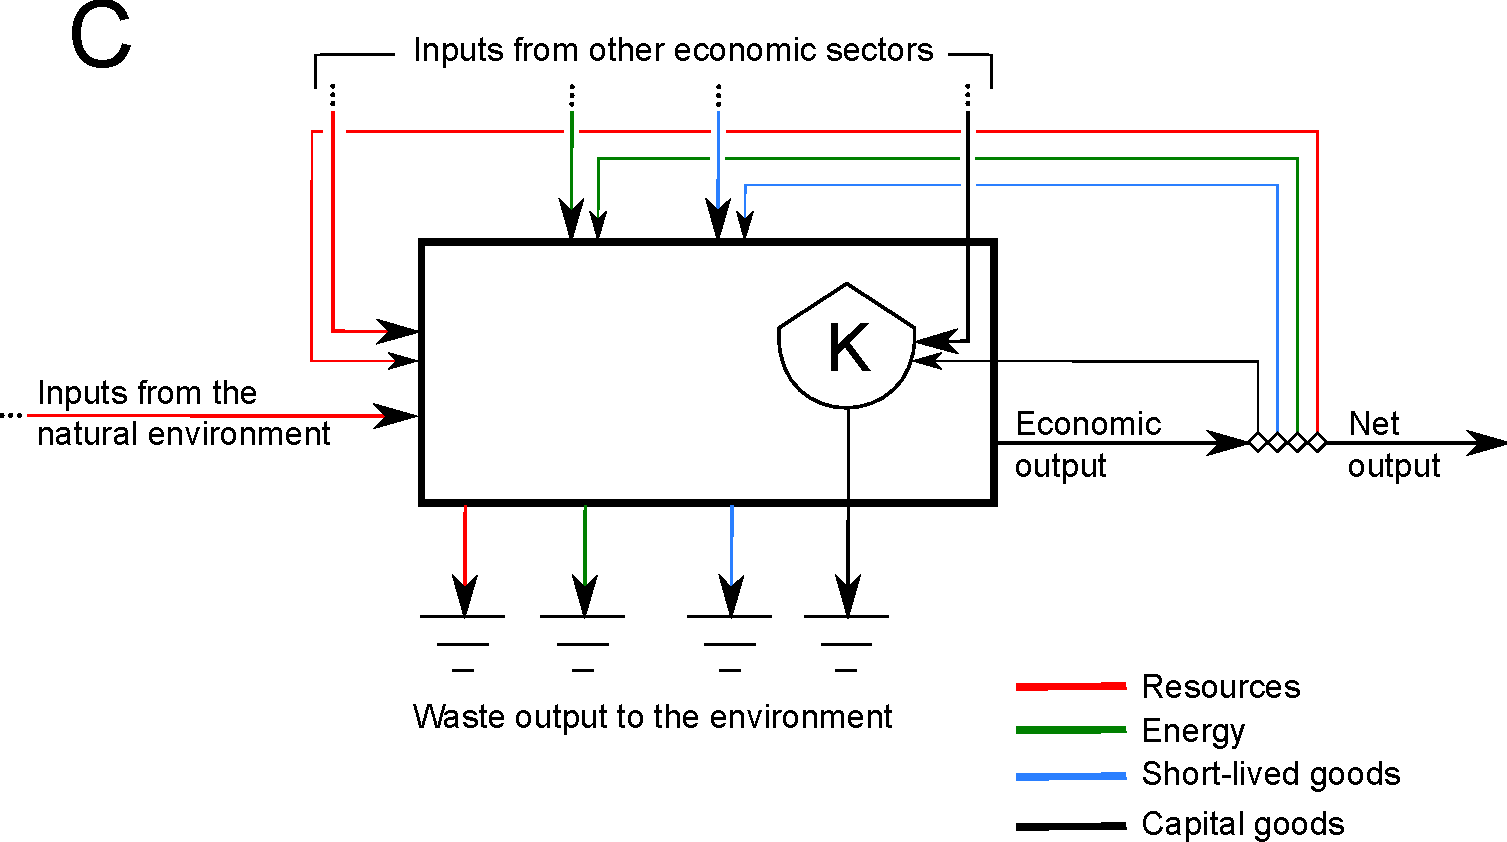
\includegraphics[width=1.0\linewidth]{Chapter_Example_D/images/Basic_unit_C.pdf}
\caption{Flows of resources (red arrows), direct energy ($\dot{E}$, green arrows), short-lived goods (blue arrows), capital goods (black arrows) and waste flows including waste heat ($\dot{Q}$) for a single economic sector. Flows of capital $\dot{K}$ are able to accumulate within the sector; no other flows may accumulate.}
\label{fig:basic_unit_C}
\end{figure}

We also introduce a distinction between two types of embodied energy flows: short-lived, non-durable goods (S), such as packaging, newspapers or the embodied energy content of direct energy flows and long-lived, durable goods (L), such as appliances, capital equipment, roads or buildings. In reality, (as the names suggest) the distinction between short- and long-lived goods is really one of degree rather than a difference in kind such that the distribution in lifetime of goods stretches from a matter of hours or days for some intermediate goods right up to thousands of years for some structures still in use today \cite{Leask2012}. We assume that there is no accumulation of short-lived goods within the economy or society, such that $\frac{\textrm{d}S}{\textrm{dt}} = 0$.  

These flows are shown in Figure XXXX for our two sector economy. Resource flows enter into the sector from the left and products leave from the right, processing flows enter from the top and waste flows leave from the bottom. We may now define the following relationships:

\begin{figure}[h!]
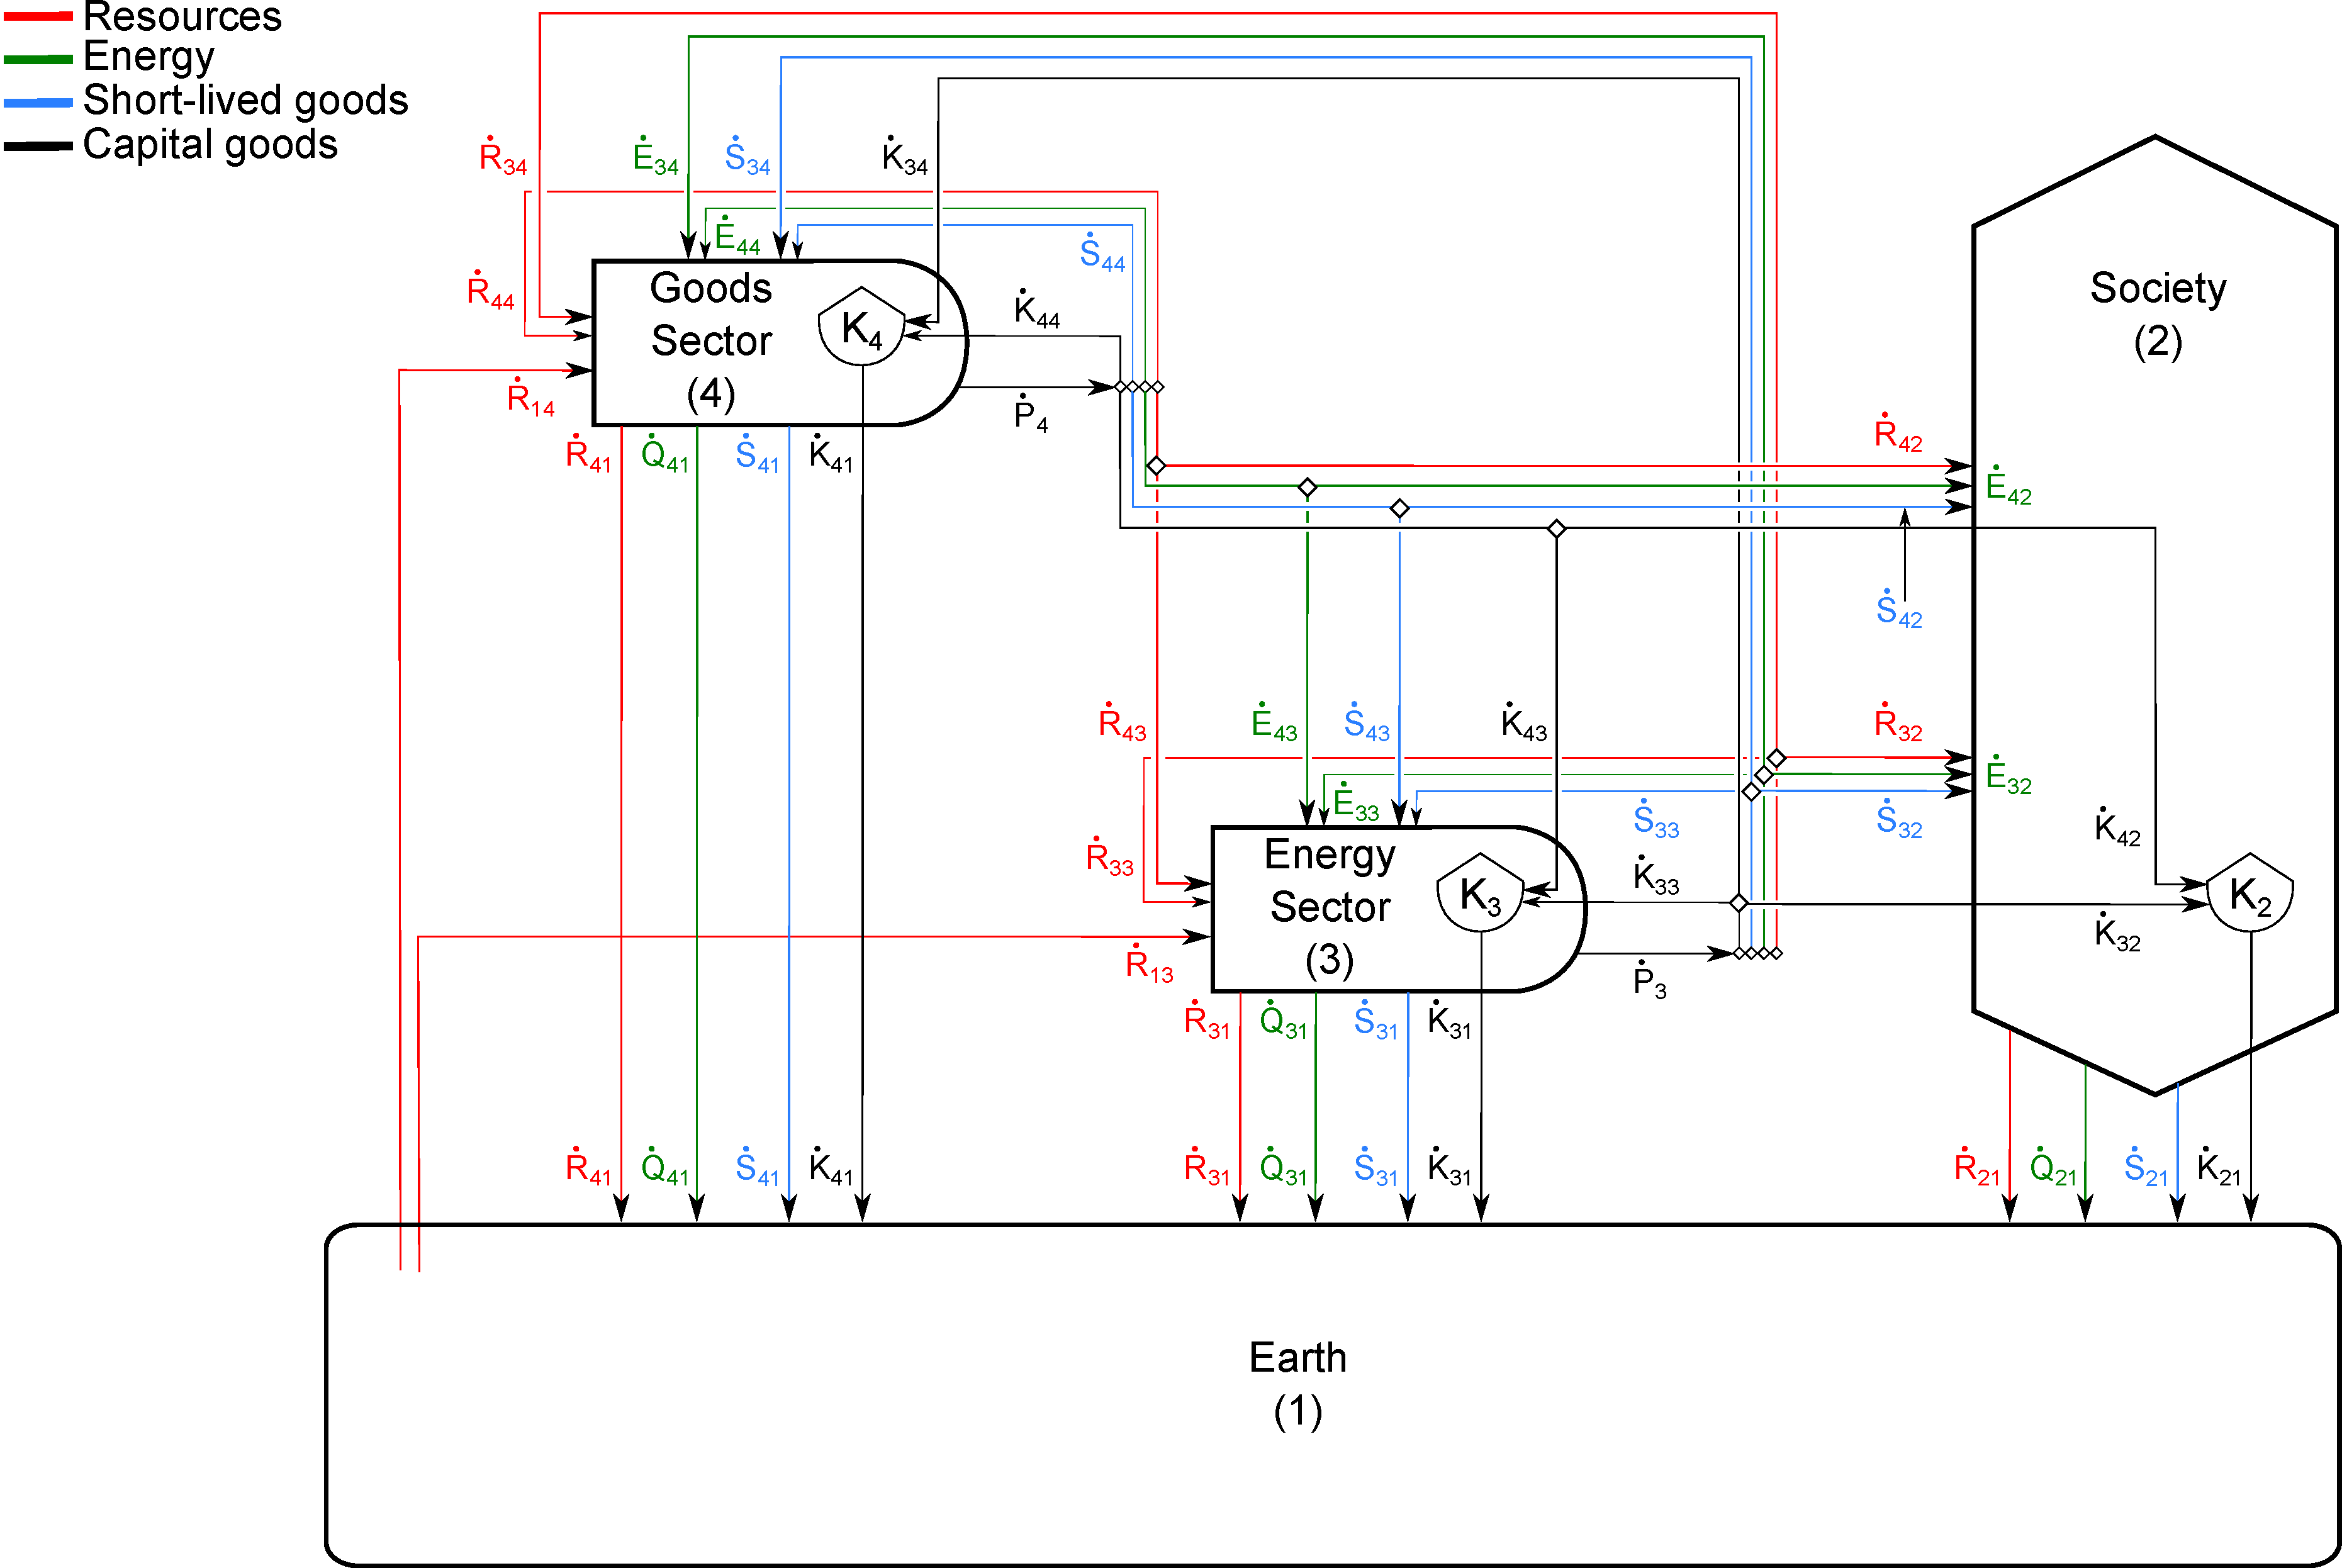
\includegraphics[width=1.0\linewidth]{Chapter_Example_D/images/PERKS_two_sector.pdf}
\caption{Flows of resources (red arrows), direct energy ($\dot{E}$, green arrows), short-lived goods (blue arrows), capital goods (black arrows) and waste flows including waste heat ($\dot{Q}$) for a two sector economy. Flows of capital $\dot{K}$ are able to accumulate within the sector; no other flows may accumulate.}
\label{fig:PERKS}
\end{figure}

\begin{equation}\label{eq:D_def_S_L}
B_{j} \equiv S_{j} + L_{j} = L_{j}
\end{equation}

%\begin{equation}\label{eq:D_def_dot_S_L}
%\dot{B} = \dot{S} + \dot{L} = \zeta\dot{B} + (1-\zeta)\dot{B}
%\end{equation}


\begin{equation}\label{eq:D_def_acc_S_L}
\frac{\textrm{d}B_{j}}{\textrm{dt}} =\frac{\textrm{d}S_{j}}{\textrm{dt}} + \frac{\textrm{d}L_{j}}{\textrm{dt}} = \frac{\textrm{d}L_{j}}{\textrm{dt}}
\end{equation}

We assume that all non-resource, energy flows $\dot{E}_{ij}$ are degraded to waste heat $\dot{Q}_{j1}$ by the processes of the sector, such that:

\begin{equation}\label{eq:D_E_balance}
\sum_{i} \dot{E}_{ij} = \dot{Q}_{j1}
\end{equation}

Similarly, we assume that all short-lived embodied energy flows $\dot{S}_{ij}$ are degraded to waste $\dot{S}_{j1}$ by the processes of the sector, such that:

\begin{equation}\label{eq:D_S_balance}
\sum_{i} \dot{S}_{ij} = \dot{S}_{j1}
\end{equation}

Since long-lived embodied energy flows, $\dot{L}_{ij}$ may accumulate with a sector, we can define that:

\begin{equation}\label{eq:D_L_balance}
\sum_{i} \dot{L}_{ij} = \dot{L}_{j1} + \frac{\textrm{d}L_{j}}{\textrm{dt}}
\end{equation}

%Given equations \ref{eq:D_E_balance} - \ref{eq:D_L_balance}, we may now stipulate that any resource flows into a sector, $\dot{R}_{ij}$, must either leave as waste flows to the earth $\dot{R}_{j1}$, or as part of the product from that sector $\dot{T}_{j}$, such that:
%
%\begin{equation}\label{eq:D_T_balance}
%\sum_{i} \dot{R}_{ij} = \dot{R}_{j1} + \dot{T}_{j}
%\end{equation}

%%%%%%%%%% Example D %%%%%%%%%%
\section{First Law of Thermodynamics}
%%%%%%%%%%

As before, the First Law of Thermodynamics requires that energy is conserved around each sector of the economy as well as around the Earth (1) and Society (2) as shown in Figure \ref{}. 

The First Law of Thermodynamics around the Earth (1), Society (2), the Energy sector (3) and Goods and Services sector (4) gives

\begin{equation} \label{eq:D-CV_E_dot_1}
	\frac{\mathrm{d}E_{1}}{\mathrm{d}t} 	 =  \dot{Q}_{21} + \dot{Q}_{31} + \dot{Q}_{41} - \dot{E}_{13} - \dot{E}_{14},
\end{equation}

\begin{equation} \label{eq:D-CV_E_dot_2}
	\frac{\mathrm{d}E_{2}}{\mathrm{d}t} 	 = \dot{E}_{32}  + \dot{E}_{42} - \dot{Q}_{21},
\end{equation}

\begin{equation} \label{eq:D-CV_E_dot_3}
	\frac{\mathrm{d}E_{3}}{\mathrm{d}t} 	 = \dot{E}_{13} + \dot{E}_{33} + \dot{E}_{43} - \dot{E}_{3} - \dot{Q}_{31}.
\end{equation}

\noindent and 

\begin{equation} \label{eq:D-CV_E_dot_4}
	\frac{\mathrm{d}E_{4}}{\mathrm{d}t} 	 = \dot{E}_{14} + \dot{E}_{34} + \dot{E}_{44} - \dot{E}_{4} - \dot{Q}_{41}.
\end{equation}

As in Examples A and B, we can set the accumulation of direct energy to zero.

\begin{equation} \label{eq:D-CV_E_dot_1_SS}
	0 =  \dot{Q}_{21} + \dot{Q}_{31} + \dot{Q}_{41} - \dot{E}_{13} - \dot{E}_{14}
\end{equation}

\begin{equation} \label{eq:D-CV_E_dot_2_SS}
	0  = \dot{E}_{32}  + \dot{E}_{42} - \dot{Q}_{21}
\end{equation}

\begin{equation} \label{eq:D-CV_E_dot_3_SS}
	0 = \dot{E}_{13} + \dot{E}_{33} + \dot{E}_{43} - \dot{E}_{3} - \dot{Q}_{31}
\end{equation}

\noindent and 

\begin{equation} \label{eq:D-CV_E_dot_4_SS}
	0 = \dot{E}_{14} + \dot{E}_{34} + \dot{E}_{44} - \dot{E}_4 - \dot{Q}_{41}
\end{equation}


%%%%%%%%%% Example D %%%%%%%%%%
\section{Total energy accounting}
%%%%%%%%%%

Accounting for accumulation of total energy and using the assumption that total energy is conserved, we can write the following equations.

\begin{equation} \label{eq:D-CV_T_1}
	\frac{\mathrm{d}T_{1}}{\mathrm{d}t} 	 = \dot{T}_{21} + \dot{T}_{31} + \dot{T}_{41} - \dot{T}_{13} - \dot{T}_{14},
\end{equation}

\begin{equation} \label{eq:D-CV_T_2}
	\frac{\mathrm{d}T_{2}}{\mathrm{d}t} 	 = \dot{T}_{32} + \dot{T}_{42} - \dot{T}_{21},
\end{equation}

\begin{equation} \label{eq:D-CV_T_3}
	\frac{\mathrm{d}T_{3}}{\mathrm{d}t} 	 = \dot{T}_{13} + \dot{T}_{33} + \dot{T}_{43} - \dot{T}_{3} - \dot{T}_{31},
\end{equation}

\noindent and 

\begin{equation} \label{eq:D-CV_T_4}
	\frac{\mathrm{d}T_{4}}{\mathrm{d}t} 	 = \dot{T}_{14} + \dot{T}_{34} + \dot{T}_{44} - \dot{T}_{4} - \dot{T}_{41}.
\end{equation}


%%%%%%%%%% Example D %%%%%%%%%%
\section{Embodied energy accounting}
%%%%%%%%%%

Given that $\frac{\mathrm{d}E_{i}}{\mathrm{d}t} = \frac{\mathrm{d}R_{i}}{\mathrm{d}t} = \frac{\mathrm{d}S_{i}}{\mathrm{d}t} = 0$, we note that $\frac{\mathrm{d}T_i}{\mathrm{d}t} = \frac{\mathrm{d}L_i}{\mathrm{d}t}$. Substituting $\dot{T} = \dot{R} + \dot{E} + \dot{S} + \dot{L}$ into the total energy accounting equations gives

\begin{equation} \label{eq:D-CV_dB_1}
	\frac{\mathrm{d}L_{1}}{\mathrm{d}t} 	 = \dot{E}_{21} + \dot{S}_{21} + \dot{L}_{21} + \dot{R}_{31} + \dot{E}_{31} + \dot{S}_{31} + \dot{L}_{31} + \dot{R}_{41} + \dot{E}_{41} + \dot{S}_{41} + \dot{L}_{41} - \dot{R}_{13} - \dot{R}_{14},
\end{equation}

\begin{equation} \label{eq:D-CV_dB_2}
	\frac{\mathrm{d}L_{2}}{\mathrm{d}t} 	 = \dot{E}_{32} + \dot{S}_{32} + \dot{L}_{32} + \dot{E}_{42} + \dot{S}_{42} + \dot{L}_{42} - \dot{E}_{21} - \dot{S}_{21} - \dot{L}_{21},
\end{equation}

\begin{equation} \label{eq:D-CV_dB_3}
	\frac{\mathrm{d}L_{3}}{\mathrm{d}t} 	 = \dot{R}_{13} + \dot{R}_{33} + \dot{E}_{33} + \dot{S}_{33} + \dot{L}_{33} + \dot{R}_{43} + \dot{E}_{43} + \dot{S}_{43} + \dot{L}_{43} - \dot{T}_{3} - \dot{R}_{31} - \dot{E}_{31} - \dot{S}_{31} - \dot{L}_{31},
\end{equation}

\noindent and 

\begin{equation} \label{eq:D-CV_dB_4}
	\frac{\mathrm{d}L_{4}}{\mathrm{d}t} 	 = \dot{R}_{14} + \dot{R}_{34} + \dot{E}_{34} + \dot{S}_{34} + \dot{L}_{34} + \dot{R}_{44} + \dot{E}_{44} + \dot{S}_{44} + \dot{L}_{44} - \dot{T}_{4} - \dot{R}_{41} - \dot{E}_{41} - \dot{S}_{41} - \dot{L}_{41}.
\end{equation}

Substituting the First Law of Thermodynamics (Equations \ref{eq:D-CV_E_dot_1_SS} through \ref{eq:D-CV_E_dot_4_SS}) into the total energy accounting equations (Equations \ref{eq:D-CV_dB_1} through \ref{eq:D-CV_dB_4}) gives embodied energy accounting equations for Example D.

\begin{equation} \label{eq:D-embodied_acct_1}
	\frac{\mathrm{d}L_{1}}{\mathrm{d}t} 	 = \dot{S}_{21} + \dot{L}_{21} + \dot{R}_{31} + \dot{S}_{31} + \dot{L}_{31} + \dot{R}_{41} +\dot{S}_{41} + \dot{L}_{41} - \dot{Q}_{21} - \dot{Q}_{31} - \dot{Q}_{41}
\end{equation}

\begin{equation} \label{eq:D-embodied_acct_2}
	\frac{\mathrm{d}L_{2}}{\mathrm{d}t} 	 = \dot{S}_{32} + \dot{L}_{32} + \dot{S}_{42} + \dot{L}_{42} + \dot{Q}_{21} - \dot{S}_{21} - \dot{L}_{21}
\end{equation}

\begin{equation} \label{eq:D-embodied_acct_3}
	\frac{\mathrm{d}L_{3}}{\mathrm{d}t} 	 = \dot{S}_{33} + \dot{L_33} + \dot{S}_{43} + \dot{L}_{43} + \dot{Q}_{31} + \dot{E}_{3} - \dot{T}_{3} - \dot{R}_{31} - \dot{S}_{31} - \dot{L}_{31}
\end{equation}

\begin{equation} \label{eq:D-embodied_acct_4}
	\frac{\mathrm{d}L_{4}}{\mathrm{d}t} 	 = \dot{S}_{34} + \dot{L_34} + \dot{S}_{44} + \dot{L}_{44} + \dot{Q}_{41} + \dot{E}_{4} - \dot{T}_{4} - \dot{R}_{41} - \dot{S}_{41} - \dot{L}_{41}
\end{equation}

[MIK ENDED HERE - MAR 27, 2013]

%Again remembering that $\frac{\textrm{d}E_{i}}{\textrm{dt}} = \dot{E}_{i1} = 0$ we can substitute \ref{eq:D_first_law} into \ref{eq:D_total_energy} to obtain:
%
%\begin{equation}\label{eq:D_emb_energy}
%\frac{\textrm{d}B_{i}}{\textrm{dt}} = \sum_{j}\dot{B}{ji} - \dot{B}_{i} - \dot{B}_{i1} + \dot{Q}_{i1}
%\end{equation}
%
%Remembering that $\frac{\textrm{d}S_{i}}{\textrm{dt}} = 0$ and $\frac{\textrm{d}B_{i}}{\textrm{dt}} = \frac{\textrm{d}S_{i}}{\textrm{dt}} + \frac{\textrm{d}L_{i}}{\textrm{dt}} = \frac{\textrm{d}L_{i}}{\textrm{dt}}$, we may simplify equation \ref{eq:D_emb_energy} to:
%
%\begin{equation}\label{eq:D_emb_energy_dL}
%\frac{\textrm{d}L_{i}}{\textrm{dt}} = \sum_{j}\dot{B}{ji} - \dot{B}_{i} - \dot{B}_{i1} + \dot{Q}_{i1}
%\end{equation}

%Given that $\frac{\mathrm{d}E_{i}}{\mathrm{d}t} = \frac{\mathrm{d}S_{i}}{\mathrm{d}t} = 0$, we again note that $\frac{\mathrm{d}T_i}{\mathrm{d}t} = \frac{\mathrm{d}B_i}{\mathrm{d}t} = \frac{\mathrm{d}L_{i}}{\mathrm{d}t}$. Substituting $\dot{T} = \dot{E} + \dot{B} = \dot{E} + \dot{S} + \dot{L}$ into the total energy accounting equations gives
%
%\begin{equation} \label{eq:D-CV_dB_1}
%	\frac{\mathrm{d}L_{1}}{\mathrm{d}t} 	 = \dot{E}_{21} + \dot{S}_{21} + \dot{L}_{21}+ \dot{E}_{31} + \dot{S}_{31} + \dot{L}_{31} + \dot{E}_{41} + \dot{S}_{41} + \dot{L}_{41} - \dot{E}_{13} - \dot{S}_{13} - \dot{L}_{13} - \dot{E}_{14} - \dot{S}_{14} - \dot{L}_{14},
%\end{equation}
%
%\begin{equation} \label{eq:D-CV_dB_2}
%	\frac{\mathrm{d}L_{2}}{\mathrm{d}t} 	 = \dot{E}_{32} + \dot{S}_{32} + \dot{L}_{32} + \dot{E}_{42} + \dot{S}_{42} + \dot{L}_{42} - \dot{E}_{21} - \dot{S}_{21} - \dot{L}_{21},
%\end{equation}
%
%\begin{equation} \label{eq:D-CV_dB_3}
%	\frac{\mathrm{d}L_{3}}{\mathrm{d}t} 	 = \dot{E}_{13} + \dot{S}_{13} + \dot{L}_{13} + \dot{E}_{33} + \dot{S}_{33} + \dot{L}_{33}+ \dot{E}_{43} + \dot{S}_{43} + \dot{L}_{43} - \dot{E}_{3} - \dot{S}_{3} - \dot{L}_{3} - \dot{E}_{31} - \dot{S}_{31} - \dot{L}_{31},
%\end{equation}
%
%\noindent and 
%
%\begin{equation} \label{eq:D-CV_dB_4}
%	\frac{\mathrm{d}L_{4}}{\mathrm{d}t} 	 = \dot{E}_{14} + \dot{S}_{14} + \dot{L}_{14} + \dot{E}_{34} + \dot{S}_{34} + \dot{L}_{34}+ \dot{E}_{44} + \dot{S}_{44} + \dot{L}_{44} - \dot{E}_{4} - \dot{S}_{4} - \dot{L}_{4} - \dot{E}_{41} - \dot{S}_{41} - \dot{L}_{41}.
%\end{equation}
%
%Substituting the First Law of Thermodynamics (Equations \ref{eq:C-CV_E_dot_1_SS} through \ref{eq:C-CV_E_dot_4_SS}) into the total energy accounting equations (Equations \ref{eq:D-CV_dB_1} through \ref{eq:D-CV_dB_4}) gives embodied energy accounting equations for Example D.
%
%\begin{equation} \label{eq:D-embodied_acct_1}
%	\frac{\mathrm{d}L_{1}}{\mathrm{d}t} 	 = \dot{S}_{21} + \dot{L}_{21} + \dot{S}_{31} + \dot{L}_{31} + \dot{S}_{41} + \dot{L}_{41} - \dot{S}_{13} - \dot{L}_{13} - \dot{S}_{14} -  \dot{L}_{14} - \dot{Q}_{21} - \dot{Q}_{31} - \dot{Q}_{41}
%\end{equation}
%
%\begin{equation} \label{eq:D-embodied_acct_2}
%	\frac{\mathrm{d}L_{2}}{\mathrm{d}t} 	 = \dot{S}_{32} +  \dot{L}_{32} + \dot{S}_{42} +  \dot{L}_{42} + \dot{Q}_{21} - \dot{S}_{21} -  \dot{L}_{21}
%\end{equation}
%
%\begin{equation} \label{eq:D-embodied_acct_3}
%	\frac{\mathrm{d}L_{3}}{\mathrm{d}t} 	 = \dot{S}_{13} +  \dot{L}_{13} + \dot{S}_{33} +  \dot{L}_{33} + \dot{S}_{43} +  \dot{L}_{43} + \dot{Q}_{31} - \dot{S}_{3} -  \dot{L}_{3} - \dot{S}_{31} -  \dot{L}_{31}
%\end{equation}
%
%\begin{equation} \label{eq:D-embodied_acct_4}
%	\frac{\mathrm{d}L_{4}}{\mathrm{d}t}	 = \dot{S}_{14} +  \dot{L}_{14} + \dot{S}_{34} +  \dot{L}_{34} + \dot{S}_{44} +  \dot{L}_{44} + \dot{Q}_{41} - \dot{S}_{4} -  \dot{L}_{4} - \dot{S}_{41} -  \dot{L}_{41}
%\end{equation}
%
%To verify the above derivation, we sum Equations \ref{eq:D-embodied_acct_1} through \ref{eq:D-embodied_acct_4} and use the following identities:
%
%\begin{equation} \label{eq:D-S_sum_3_output}
%	\dot{S}_3 = \dot{S}_{32} + \dot{S}_{33} + \dot{S}_{34}
%\end{equation}
%
%\begin{equation} \label{eq:D-L_sum_3_output}
%	\dot{L}_3 = \dot{L}_{32} + \dot{L}_{33} + \dot{L}_{34}
%\end{equation}
%
%\begin{equation} \label{eq:D-S_sum_4_output}
%	\dot{S}_4 = \dot{S}_{42} + \dot{S}_{43} + \dot{S}_{44};
%\end{equation}
%
%\noindent and
%
%\begin{equation} \label{eq:D-L_sum_4_output}
%	\dot{L}_4 = \dot{L}_{42} + \dot{L}_{43} + \dot{L}_{44};
%\end{equation}
%
%\noindent to obtain
%
%\begin{equation} \label{eq:D-B_sums_to_zero}
%	\frac{\mathrm{d}B_{1}}{\mathrm{d}t} + \frac{\mathrm{d}B_{2}}{\mathrm{d}t} + \frac{\mathrm{d}B_{3}}{\mathrm{d}t} + \frac{\mathrm{d}B_{4}}{\mathrm{d}t} = 0
%\end{equation}
%
%\noindent as expected. The total embodied energy content of the system (Earth (1), Society (2), Energy sector (3), and Goods and Services sector (4)) is constant with respect to time.

%%%%%%%%%% Example D %%%%%%%%%%
 \section{Depreciation}
%%%%%%%%%%


The term $\dot{B}_{i1}$ represents material depreciation (i.e., disposal) rates. There are two components to this disposal of embodied energy: the first is disposal of short-lived goods, $S_{i1}$, the second is depreciation of long-lived capital, $L_{i1} = \gamma_i L_i$. We may now substitute these into equation \ref{eq:D_emb_energy_dL} to obtain:

\begin{equation}\label{eq:D_dep}
\frac{\textrm{d}L_{i}}{\textrm{dt}} = \sum_{j}\dot{B}{ji} - \dot{B}_{i} - \dot{S}_{i1} - \gamma_i L_i + \dot{Q}_{i1}
\end{equation}

%We can represent the embodied energy content of material depreciation as $\dot{B}_{i1} = \gamma_i B_i = \gamma_i (S_i + L_i)$. Realizing that $S_i = 0$ we can see that $\gamma_i B_i = \gamma_i L_i$ which we may use to obtain:
%
%\begin{equation} \label{eq:D-embodied_acct_1_depreciation}
%	\frac{\mathrm{d}L_{1}}{\mathrm{d}t} 	 = \dot{S}_{21} + \gamma_2 L_2 + \dot{S}_{31} + \gamma_3 L_3 + \dot{S}_{41} + \gamma_4 L_4 - \dot{S}_{13} - \dot{L}_{13} - \dot{S}_{14} - \dot{L}_{14} - \dot{Q}_{21} - \dot{Q}_{31} - \dot{Q}_{41}
%\end{equation}
%
%\begin{equation} \label{eq:D-embodied_acct_2_depreciation}
%	\frac{\mathrm{d}L_{2}}{\mathrm{d}t} 	 = \dot{S}_{32} + \dot{L}_{32} + \dot{S}_{42} + \dot{L}_{42} + \dot{Q}_{21} - \dot{S}_{21} - \gamma_2 L_2
%\end{equation}
%
%\begin{equation} \label{eq:D-embodied_acct_3_depreciation}
%	\frac{\mathrm{d}L_{3}}{\mathrm{d}t} 	 = \dot{S}_{13} + \dot{L}_{13} + \dot{S}_{33} + \dot{L}_{33} + \dot{S}_{43} + \dot{L}_{43} + \dot{Q}_{31} - \dot{S}_{3} - \dot{L}_{3} - \dot{S}_{31} - \gamma_3 L_3
%\end{equation}
%
%\begin{equation} \label{eq:D-embodied_acct_4_depreciation}
%	\frac{\mathrm{d}L_{4}}{\mathrm{d}t}	 = \dot{S}_{14} + \dot{L}_{14} + \dot{S}_{34} + \dot{L}_{34} + \dot{S}_{44} + \dot{L}_{44} + \dot{Q}_{41} - \dot{S}_{4} - \dot{L}_{4} - \dot{S}_{41} - \gamma_4 L_4
%\end{equation}


%%%%%%%%%% Example D %%%%%%%%%%
\section{Final demand}
%%%%%%%%%%

Society's demand vector for total energy, $\dot{T}$, can again be written as 

\begin{equation} \label{eq:D-demand_vector_T_dot}
	\vec{Y}_{\dot{T}} = 	\begin{Bmatrix} 	\dot{T}_{32}	\\
																\dot{T}_{42}	\\
									\end{Bmatrix}.
\end{equation}

\noindent In terms of total energy, the ultimate demand ($Y_{\dot{T}}$) is given by 

\begin{equation} \label{eq:D-final_demand_T_sum}
	Y_{\dot{T}} = 	\sum_{i=3}^{N} \dot{T}_{i2} = \dot{T}_{32} + \dot{B}_{42} = \dot{T}_{32} + \dot{S}_{42} + \dot{L}_{42}.
\end{equation}

\noindent after realizing that $\dot{E}_{42} = 0$.

Using $\dot{T}_{32} = \dot{E}_{32} + \dot{S}_{32} + \dot{L}_{32}$ and rearranging Equation \ref{eq:D-final_demand_T_sum} gives

\begin{equation} \label{eq:D-rearranged_final_demand_T_sum}
	\dot{S}_{32} +\dot{L}_{32} + \dot{S}_{42} + \dot{L}_{42} = Y_{\dot{T}} - \dot{E}_{32}.
\end{equation}

\noindent Substituting Equation \ref{eq:D-rearranged_final_demand_T_sum} into Equation \ref{eq:D-embodied_acct_2_depreciation} yields

\begin{equation} \label{eq:D-intermediate_T_sum_dB2_dt}
	\frac{\mathrm{d}L_2}{\mathrm{d}t} = Y_{\dot{T}} - \dot{E}_{32} + \dot{Q}_{21} - \dot{S}_{21} - \gamma_2 L_2.
\end{equation}

Substituting Equation \ref{eq:C-CV_E_dot_2_SS} into Eqaution \ref{eq:D-intermediate_T_sum_dB2_dt} and realizing that $\dot{E}_{42} = 0$ because direct energy is supplied to society by the energy sector only, we obtain 

\begin{equation} \label{eq:D-compare_demand_and_accumulation}
	\frac{\mathrm{d}L_{2}}{\mathrm{d}t} = Y_{\dot{T}} - \dot{S}-{21} - \gamma_{2}L_{2},
\end{equation}

\noindent indicating that the final demand vector for total energy ($Y_{\dot{T}}$) and the accumulation rate of energy in society $\left(\frac{\mathrm{d}L_{2}}{\mathrm{d}t}\right)$ differ by the rate of disposal from society ($\gamma_{2}L_{2}$). We note that as total embodied energy in society ($B_{2}$) becomes increasingly large, we need an ever-increasing rate of energy supplied to the society ($Y_{\dot{T}}$) to maintain positive growth $\left(\frac{\mathrm{d}L_{2}}{\mathrm{d}t}\right)$. 

%%%%%%%%%% Example D %%%%%%%%%%
\section{Flows of Value ($\dot{X}$)}
%%%%%%%%%%

The following figure shows value flows ($\dot{X}$) in the two-sector economy.

Realizing that the valuable output from energy sectors is direct energy, $\dot{X}_{3} = \dot{E}_{3}$ and $\dot{X}_{3j} = \dot{E}_{3j}$. Thus, outputs from energy sectors are given in energy units (joules or BTUs). 

Written in terms of value flows, the ultimate demand vector ($\vec{Y}$) is given by

\begin{equation} \label{eq:D-demand_vector_B_dot}
	\vec{Y}_{\dot{X}} = 	\begin{Bmatrix} 	\dot{X}_{32}	\\
																\dot{X}_{42}	\\
									\end{Bmatrix},
\end{equation}

\noindent and the total value demand from society ($Y$) is 

\begin{equation} \label{eq:D-total_value_demand}
	Y_{\dot{X}} = \sum_{i=1}^{N} \dot{X}_{i2} = \dot{X}_{32} + \dot{X}_{42}.
	\end{equation}

%%%%%%%%%% Example D %%%%%%%%%%
\section{Matrix Formulation}
%%%%%%%%%%

We can use Equations \ref{eq:epsilon_output_def} through \ref{eq:epsilon_equiv_1} to rewrite Equations \ref{eq:D-CV_B_1_depreciation} and \ref{eq:D-CV_B_2_depreciation} as

\begin{equation} \label{eq:D-CV_B_3_with_eps}
	\dot{X}_{33}\varepsilon_{3} + \dot{X}_{43}\varepsilon_{4} + \dot{E}_{13} - \frac{\mathrm{d}L_{3}}{\mathrm{d}t} - \dot{S}_{31} - \gamma_{3}L_{3} = \dot{X}_{3}\varepsilon_{3}
\end{equation}

\noindent and 

\begin{equation} \label{eq:D-CV_B_4_with_eps}
	\dot{X}_{34}\varepsilon_{3} + \dot{X}_{44}\varepsilon_{4} + \dot{E}_{14} - \frac{\mathrm{d}L_{4}}{\mathrm{d}t} - \dot{S}_{41} - \gamma_{4}L_{4} = \dot{X}_{4}\varepsilon_{4}.
\end{equation}

We can rewrite Equations \ref{eq:D-CV_B_3_with_eps} and \ref{eq:D-CV_B_4_with_eps} in matrix notation with the following definitions:

\begin{equation} \label{eq:D-eps_vec_def}
	\vec{\varepsilon} =		\begin{Bmatrix} 	\varepsilon_{3}	\\
																\varepsilon_{4}	\\
									\end{Bmatrix},
\end{equation}

\begin{equation} \label{eq:D-E_vec_def}
	\vec{E} =		\begin{Bmatrix} 	\dot{E}_{13}	\\
													\dot{E}_{14}\\
						\end{Bmatrix},
\end{equation}

\begin{equation} \label{eq:D-dLdt_vec_def}
	\frac{\mathrm{d}\vec{L}}{\mathrm{d}t} =	\begin{Bmatrix}	\frac{\mathrm{d}L_{3}}{\mathrm{d}t}	\\
																									\frac{\mathrm{d}L_{4}}{\mathrm{d}t}\\
																		\end{Bmatrix},
\end{equation}

\begin{equation} \label{eq:B_vec_def}
	\vec{B} =	\vec{L} =		\begin{Bmatrix}	L_{3}\\
																	L_{4}\\
										\end{Bmatrix},
\end{equation}

\begin{equation} \label{eq:D-A_matrix_def}
	\vec{A} =	\begin{bmatrix} 	a_{33} & a_{34}	\\
												a_{43} & a_{44}	\\
					\end{bmatrix},
\end{equation}

\begin{equation} \label{eq:D-X_t_matrix_def}
	\vec{X}_{t} =		\begin{bmatrix} 	\dot{X}_{33}		&	\dot{X}_{34}	\\
														\dot{X}_{43}		&	\dot{X}_{44}\\
							\end{bmatrix},
\end{equation}

\begin{equation} \label{eq:D-X_hat_matrix_def}
	\hat{\vec{X}} = \delta_{ij}\dot{X}_{j} = \begin{bmatrix} 	\dot{X}_{33}		&	0					\\
																								0					&	\dot{X}_{44}	\\
																							\end{bmatrix},
\end{equation}


\begin{equation} \label{eq:D-B_hat_matrix_def}
	\hat{\vec{\gamma}} = \delta_{ij}\gamma_{j},
\end{equation}

\noindent and

\begin{equation} \label{eq:D-S_vec_def}
	\vec{S} =		\begin{Bmatrix} 	\dot{S}_{31}	\\
													\dot{S}_{41}\\
						\end{Bmatrix},
\end{equation}

\noindent such that:

\begin{equation} \label{D-eq:matrix_leontief}
	\vec{X}_{t}^{\mathrm{T}}\vec{\varepsilon} + \vec{E} - \left(\frac{\mathrm{d}\vec{L}}{\mathrm{d}t} +\vec{S} + \hat{\vec{\gamma}}\vec{L}\right) = \hat{\vec{X}}\vec{\varepsilon}.
\end{equation}

%%%%%%%%%% Example D %%%%%%%%%%
\section{Estimating $\vec{\varepsilon}$ and $\frac{\mathrm{d}\vec{B}}{\mathrm{d}t}$}
%%%%%%%%%%

With Equation \ref{eq:D-matrix_leontief}, we can solve for either the energy accumulation vector ($\vec{\frac{\mathrm{d}L}{\mathrm{d}t}}$) or the energy intensity vector ($\vec{\varepsilon}$), but not both. 

Solving for the accumulation vector gives

\begin{equation} \label{eq:D-dL_dt_leontief}
	\frac{\mathrm{d}\vec{L}}{\mathrm{d}t} = (\vec{X}_{t}^{\mathrm{T}} - \hat{\vec{X}})\vec{\varepsilon} + \vec{E} - \vec{S} - \hat{\vec{\gamma}}\vec{L}.
\end{equation}

\noindent Finally, we can substutute Equation \ref{eq:Xdifference1} which gives

\begin{equation} \label{eq:D-dB_dt_leontief_with_A}
	\frac{\mathrm{d}\vec{L}}{\mathrm{d}t} = \hat{\vec{X}} (\vec{A}^{\mathrm{T}} - \vec{I}) \vec{\varepsilon} + \vec{E} - \vec{S} - \hat{\vec{\gamma}}\vec{L},
\end{equation}

\noindent which allows estimation of the accumulation of long-lived goods in economic sectors $\left(\frac{\mathrm{d}\vec{L}}{\mathrm{d}t}\right)$ knowing only sector outputs ($\hat{\vec{X}}$), sector input-output ratios ($\vec{A}$), sector energy intensities ($\vec{\varepsilon}$), energy input to the economy ($\vec{E}$), and sector physical depreciation rates ($\hat{\vec{\gamma}}\vec{L}$). In theory, the transaction matrix ($\vec{X}_{t}$) is not required if the input-ouput ratios ($\vec{A}$) are known, though in reality, knowledge of input-output ratios would be derived from the transaction matrix $\vec{X}_{t}$ .

Solving for the energy intensity vector gives

\begin{equation} \label{eq:D-epsilon_leontief}
	\vec{\varepsilon} = (\hat{\vec{X}} - \vec{X}_{t}^{\mathrm{T}})^{-1}\left[\vec{E} - \left(\frac{\mathrm{d}\vec{L}}{\mathrm{d}t} + \vec{S} + \hat{\vec{\gamma}}\vec{L}\right)\right].
\end{equation}

\noindent Substituting Equation \ref{eq:Xdifference2_inverse} gives

\begin{equation} \label{eq:D-epsilon_leontief_with_A}
	\vec{\varepsilon} = (\vec{I} - \vec{A}^{\mathrm{T}})^{-1}\hat{\vec{X}}^{-1}\left[\vec{E} - \left(\frac{\mathrm{d}\vec{L}}{\mathrm{d}t} + \vec{S} + \hat{\vec{\gamma}}\vec{L}\right)\right],
\end{equation}

\noindent which allows estimation of the energy intensity of economic sectors ($\vec{\varepsilon}$) knowing only sector input-output ratios ($\vec{A}$), sector outputs ($\hat{\vec{X}}$), energy input to the economy ($\vec{E}$), sector embodied energy accumulation rates $\left(\frac{\mathrm{d}\vec{L}}{\mathrm{d}t}\right)$, and sector physical depreciation rates ($\hat{\vec{\gamma}}\vec{L}$).

Comparison of Equations \ref{eq:eps1_ss_IO} and \ref{eq:epsilon_leontief_with_A} shows the similarities between the single-sector algebraic formulation and the multi-sector matrix formulation of the I-O analysis method. This newly developed multi-sector matrix formulation can be extended to any desired level of economic and energy sector disaggregation as shown by Bullard (1975, 1978) and others.


\bibliography{EROI_review_v2}
\bibliographystyle{unsrt}


% Always give a unique label
% and use \ref{<label>} for cross-references
% and \cite{<label>} for bibliographic references
% use \sectionmark{}
% to alter or adjust the section heading in the running head
%% Instead of simply listing headings of different levels we recommend to let every heading be followed by at least a short passage of text. Furtheron please use the \LaTeX\ automatism for all your cross-references and citations.

%% Please note that the first line of text that follows a heading is not indented, whereas the first lines of all subsequent paragraphs are.

%% Use the standard \verb|equation| environment to typeset your equations, e.g.
%
%% \begin{equation}
%% a \times b = c\;,
%% \end{equation}
%
%% however, for multiline equations we recommend to use the \verb|eqnarray|
%% environment\footnote{In physics texts please activate the class option \texttt{vecphys} to depict your vectors in \textbf{\itshape boldface-italic} type - as is customary for a wide range of physical subjects.}.
%% \begin{eqnarray}
%% a \times b = c \nonumber\\
%% \vec{a} \cdot \vec{b}=\vec{c}
%% \label{eq:01}
%% \end{eqnarray}

%% \subsection{Subsection Heading}
%% \label{subsec:2}
%% Instead of simply listing headings of different levels we recommend to let every heading be followed by at least a short passage of text. Furtheron please use the \LaTeX\ automatism for all your cross-references\index{cross-references} and citations\index{citations} as has already been described in Sect.~\ref{sec:2}.

%% \begin{quotation}
%% Please do not use quotation marks when quoting texts! Simply use the \verb|quotation| environment -- it will automatically render Springer's preferred layout.
%% \end{quotation}


%% \subsubsection{Subsubsection Heading}
%% Instead of simply listing headings of different levels we recommend to let every heading be followed by at least a short passage of text. Furtheron please use the \LaTeX\ automatism for all your cross-references and citations as has already been described in Sect.~\ref{subsec:2}, see also Fig.~\ref{fig:1}\footnote{If you copy text passages, figures, or tables from other works, you must obtain \textit{permission} from the copyright holder (usually the original publisher). Please enclose the signed permission with the manucript. The sources\index{permission to print} must be acknowledged either in the captions, as footnotes or in a separate section of the book.}

%% Please note that the first line of text that follows a heading is not indented, whereas the first lines of all subsequent paragraphs are.

% For figures use
%
%% \begin{figure}[b]
%% \sidecaption
% Use the relevant command for your figure-insertion program
% to insert the figure file.
% For example, with the option graphics use
%% \includegraphics[scale=.65]{figure}
%
% If not, use
%\picplace{5cm}{2cm} % Give the correct figure height and width in cm
%
%% \caption{If the width of the figure is less than 7.8 cm use the \texttt{sidecapion} command to flush the caption on the left side of the page. If the figure is positioned at the top of the page, align the sidecaption with the top of the figure -- to achieve this you simply need to use the optional argument \texttt{[t]} with the \texttt{sidecaption} command}
%% \label{fig:1}       % Give a unique label
%% \end{figure}


%% \paragraph{Paragraph Heading} %
%% Instead of simply listing headings of different levels we recommend to let every heading be followed by at least a short passage of text. Furtheron please use the \LaTeX\ automatism for all your cross-references and citations as has already been described in Sect.~\ref{sec:2}.

%% Please note that the first line of text that follows a heading is not indented, whereas the first lines of all subsequent paragraphs are.

%% For typesetting numbered lists we recommend to use the \verb|enumerate| environment -- it will automatically render Springer's preferred layout.

%% \begin{enumerate}
%% \item{Livelihood and survival mobility are oftentimes coutcomes of uneven socioeconomic development.}
%% \begin{enumerate}
%% \item{Livelihood and survival mobility are oftentimes coutcomes of uneven socioeconomic development.}
%% \item{Livelihood and survival mobility are oftentimes coutcomes of uneven socioeconomic development.}
%% \end{enumerate}
%% \item{Livelihood and survival mobility are oftentimes coutcomes of uneven socioeconomic development.}
%% \end{enumerate}


%% \subparagraph{Subparagraph Heading} In order to avoid simply listing headings of different levels we recommend to let every heading be followed by at least a short passage of text. Use the \LaTeX\ automatism for all your cross-references and citations as has already been described in Sect.~\ref{sec:2}, see also Fig.~\ref{fig:2}.

%% Please note that the first line of text that follows a heading is not indented, whereas the first lines of all subsequent paragraphs are.

%% For unnumbered list we recommend to use the \verb|itemize| environment -- it will automatically render Springer's preferred layout.

%% \begin{itemize}
%% \item{Livelihood and survival mobility are oftentimes coutcomes of uneven socioeconomic development, cf. Table~\ref{tab:1}.}
%% \begin{itemize}
%% \item{Livelihood and survival mobility are oftentimes coutcomes of uneven socioeconomic development.}
%% \item{Livelihood and survival mobility are oftentimes coutcomes of uneven socioeconomic development.}
%% \end{itemize}
%% \item{Livelihood and survival mobility are oftentimes coutcomes of uneven socioeconomic development.}
%% \end{itemize}

%% \begin{figure}[t]
%% \sidecaption[t]
% Use the relevant command for your figure-insertion program
% to insert the figure file.
% For example, with the option graphics use
%% \includegraphics[scale=.65]{figure}
%
% If not, use
%\picplace{5cm}{2cm} % Give the correct figure height and width in cm
%
%% \caption{Please write your figure caption here}
%% \label{fig:2}       % Give a unique label
%% \end{figure}

%% \runinhead{Run-in Heading Boldface Version} Use the \LaTeX\ automatism for all your cross-references and citations as has already been described in Sect.~\ref{sec:2}.

%% \subruninhead{Run-in Heading Italic Version} Use the \LaTeX\ automatism for all your cross-refer\-ences and citations as has already been described in Sect.~\ref{sec:2}\index{paragraph}.
% Use the \index{} command to code your index words
%
% For tables use
%
%% \begin{table}
%% \caption{Please write your table caption here}
%% \label{tab:1}       % Give a unique label
%
% For LaTeX tables use
%
%% \begin{tabular}{p{2cm}p{2.4cm}p{2cm}p{4.9cm}}
%% \hline\noalign{\smallskip}
%% Classes & Subclass & Length & Action Mechanism  \\
%% \noalign{\smallskip}\svhline\noalign{\smallskip}
%% Translation & mRNA$^a$  & 22 (19--25) & Translation repression, mRNA cleavage\\
%% Translation & mRNA cleavage & 21 & mRNA cleavage\\
%% Translation & mRNA  & 21--22 & mRNA cleavage\\
%%Translation & mRNA  & 24--26 & Histone and DNA Modification\\
%%\noalign{\smallskip}\hline\noalign{\smallskip}
%%\end{tabular}
%%$^a$ Table foot note (with superscript)
%%\end{table}
%
%% \section{Section Heading}
%%\label{sec:3}
% Always give a unique label
% and use \ref{<label>} for cross-references
% and \cite{<label>} for bibliographic references
% use \sectionmark{}
% to alter or adjust the section heading in the running head
%% Instead of simply listing headings of different levels we recommend to let every heading be followed by at least a short passage of text. Furtheron please use the \LaTeX\ automatism for all your cross-references and citations as has already been described in Sect.~\ref{sec:2}.

%% Please note that the first line of text that follows a heading is not indented, whereas the first lines of all subsequent paragraphs are.

%%If you want to list definitions or the like we recommend to use the Springer-enhanced \verb|description| environment -- it will automatically render Springer's preferred layout.

%%\begin{description}[Type 1]
%%\item[Type 1]{That addresses central themes pertainng to migration, health, and disease. In Sect.~\ref{sec:1}, Wilson discusses the role of human migration in infectious disease distributions and patterns.}
%%\item[Type 2]{That addresses central themes pertainng to migration, health, and disease. In Sect.~\ref{subsec:2}, Wilson discusses the role of human migration in infectious disease distributions and patterns.}
%%\end{description}

%%\subsection{Subsection Heading} %
%% In order to avoid simply listing headings of different levels we recommend to let every heading be followed by at least a short passage of text. Use the \LaTeX\ automatism for all your cross-references and citations citations as has already been described in Sect.~\ref{sec:2}.

%% Please note that the first line of text that follows a heading is not indented, whereas the first lines of all subsequent paragraphs are.

%% \begin{svgraybox}
%% If you want to emphasize complete paragraphs of texts we recommend to use the newly defined Springer class option \verb|graybox| and the newly defined environment \verb|svgraybox|. This will produce a 15 percent screened box 'behind' your text.

%% If you want to emphasize complete paragraphs of texts we recommend to use the newly defined Springer class option and environment \verb|svgraybox|. This will produce a 15 percent screened box 'behind' your text.
%% \end{svgraybox}


%% \subsubsection{Subsubsection Heading}
%%Instead of simply listing headings of different levels we recommend to let every heading be followed by at least a short passage of text. Furtheron please use the \LaTeX\ automatism for all your cross-references and citations as has already been described in Sect.~\ref{sec:2}.

%% Please note that the first line of text that follows a heading is not indented, whereas the first lines of all subsequent paragraphs are.

%% \begin{theorem}
%% Theorem text goes here.
%% \end{theorem}
%
% or
%
%% \begin{definition}
%% Definition text goes here.
%% \end{definition}

%% \begin{proof}
%\smartqed
%% Proof text goes here.
%% \qed
%% \end{proof}

%%\paragraph{Paragraph Heading} %
%% Instead of simply listing headings of different levels we recommend to let every heading be followed by at least a short passage of text. Furtheron please use the \LaTeX\ automatism for all your cross-references and citations as has already been described in Sect.~\ref{sec:2}.

%% Note that the first line of text that follows a heading is not indented, whereas the first lines of all subsequent paragraphs are.
%
% For built-in environments use
%
%%\begin{theorem}
%%Theorem text goes here.
%%\end{theorem}
%
%%\begin{definition}
%%Definition text goes here.
%%\end{definition}
%
%%\begin{proof}
%%\smartqed
%% Proof text goes here.
%%\qed
%%\end{proof}
%
%% \begin{acknowledgement}
%% If you want to include acknowledgments of assistance and the like at the end of an individual chapter please use the \verb|acknowledgement| environment -- it will automatically render Springer's preferred layout.
%% \end{acknowledgement}
%
%% \section*{Appendix}
%% \addcontentsline{toc}{section}{Appendix}
%
%% When placed at the end of a chapter or contribution (as opposed to at the end of the book), the numbering of tables, figures, and equations in the appendix section continues on from that in the main text. Hence please \textit{do not} use the \verb|appendix| command when writing an appendix at the end of your chapter or contribution. If there is only one the appendix is designated ``Appendix'', or ``Appendix 1'', or ``Appendix 2'', etc. if there is more than one.

%% \begin{equation}
%% a \times b = c
%% \end{equation}
% Problems or Exercises should be sorted chapterwise
%% \section*{Problems}
%% \addcontentsline{toc}{section}{Problems}
%
% Use the following environment.
% Don't forget to label each problem;
% the label is needed for the solutions' environment
%% \begin{prob}
%% \label{prob1}
%% A given problem or Excercise is described here. The
%% problem is described here. The problem is described here.
%% \end{prob}

%% \begin{prob}
%% \label{prob2}
%% \textbf{Problem Heading}\\
%% (a) The first part of the problem is described here.\\
%% (b) The second part of the problem is described here.
%% \end{prob}




%!TEX root = ../../Heun_Dale_Haney_A_dynamic_approach_to_input_output_modeling.tex
%%%%%%%%%%%%%%%%%%%%% chapter.tex %%%%%%%%%%%%%%%%%%%%%%%%%%%%%%%%%
%
% sample chapter
%
% Use this file as a template for your own input.
%
%%%%%%%%%%%%%%%%%%%%%%%% Springer-Verlag %%%%%%%%%%%%%%%%%%%%%%%%%%
%\motto{Use the template \emph{chapter.tex} to style the various elements of your chapter content.}

\motto{Development without growth beyond the earth's carrying capacity is true progress.~\emph{\cite{Daly:2012aa}}

\hfill---\emph{Herman Daly}}


%%%%%%%%%%%%%%%%%%%%%%%%%%%%%%%%%%
%%%%%%%%%% Implications %%%%%%%%%%
%%%%%%%%%%%%%%%%%%%%%%%%%%%%%%%%%%
\chapter{Implications}
% Always give a unique label
\label{chap:implications}
% use \chaptermark{} to alter or adjust the chapter heading in the running head
\chaptermark{Implications}
%%%%%%%%%%%%%%%%%%%%%%%%%%%%%%%%%%
%%%%%%%%%%%%%%%%%%%%%%%%%%%%%%%%%%
%%%%%%%%%%%%%%%%%%%%%%%%%%%%%%%%%%


%% \abstract{Each chapter should be preceded by an abstract (10--15 lines long) that summarizes the content. The abstract will appear \textit{online} at \url{www.SpringerLink.com} and be available with unrestricted access. This allows unregistered users to read the abstract as a teaser for the complete chapter. As a general rule the abstracts will not appear in the printed version of your book unless it is the style of your particular book or that of the series to which your book belongs.\newline\indent
%% Please use the 'starred' version of the new Springer \texttt{abstract} command for typesetting the text of the online abstracts (cf. source file of this chapter template \texttt{abstract}) and include them with the source files of your manuscript. Use the plain \texttt{abstract} command if the abstract is also to appear in the printed version of the book.}

%% Use the template \emph{chapter.tex} together with the Springer document class SVMono (monograph-type books) or SVMult (edited books) to style the various elements of your chapter content in the Springer layout.

\abstract*{In this chapter, we discuss several implications that arise from 
the detailed development of our dynamic framework for material,
energy, and value accounting.
The first implications are for the energy I-O method itself. 
We recommend a physical accounting framework that fully
accounts for capital stock and energy input from society (final consumption)
to the economy.
We then discuss implications for economic ``development,''
namely that economic growth could be considered a ``fully coupled'' problem: 
understanding it requires breadth of knowledge 
and appreciation for interactions among many important factors,
including financial capital, physical capital and associated ambodied energy,
direct energy, resources, and societal inputs.
Each, alone, is necessary, but not sufficient, for economic development.
We discuss implications for recycling and reuse of materials
as well as the concept of dematerialziation.
Finally, we view the concept of a steady-state economy through
the lens of our framework.
We find that there are many potential definitions of a steady-state economy,
none of which are fully satisfying when compared against the ideal 
of sustainability.}


Several implications can be drawn from the detailed development 
of our framework for materials, energy, and value accounting 
(in Chapters~\ref{chap:materials}--\ref{chap:intensity}).
In the sections below, we discuss 
implications for the Energy Input-Output (EI-O) method itself,
implications for economic ``development,''
implications for recycling, reuse, and dematerialization, and
comparisons between our framework and the notion of a steady-state economy.
We begin by examining the EI-O method 
through the lens of our framework.


%%%%%%%%%% Implications for the I-O method %%%%%%%%%%
\section{Implications for the I-O method}
\label{sec:Implications_for_IO}
%%%%%%%%%%

Extension of the Leontief
Input-Output method
for energy analysis has allowed energy analysts to estimate 
the energy intensity
of economic products~($\boldsymbol{\varepsilon}$). 
As discussed in Section~\ref{sec:Value_Methodology},
we do not take the ability to estimate energy intensity as a license
to declare an intrinsic ``energy theory of value.''
Rather, we belive that energy intensity~($\boldsymbol{\varepsilon}$) is an 
important and useful metric that can assess 
the energy performance of economies,
even within the prevailing subjective theory of value
that underlies modern economics.
It is important to consider the assumptions behind
the literature's presentation of the EI-O method 
for estimating the energy intensity of economic output
before drawing implications from our framework.

As we investigate, we will use the following
coordinates of analysis:
product-based vs.\ physical accounting frameworks,
whether capital stock is included in the accounting framework, and
whether energy input from society to the economy is included.
(See Figure~\ref{fig:coords_of_analysis}.)
We will end with our suggestion for how best to estimate
$\boldsymbol{\varepsilon}$ within
a materials, energy, and value accounting framework.

\begin{figure}[!ht]
\centering{}
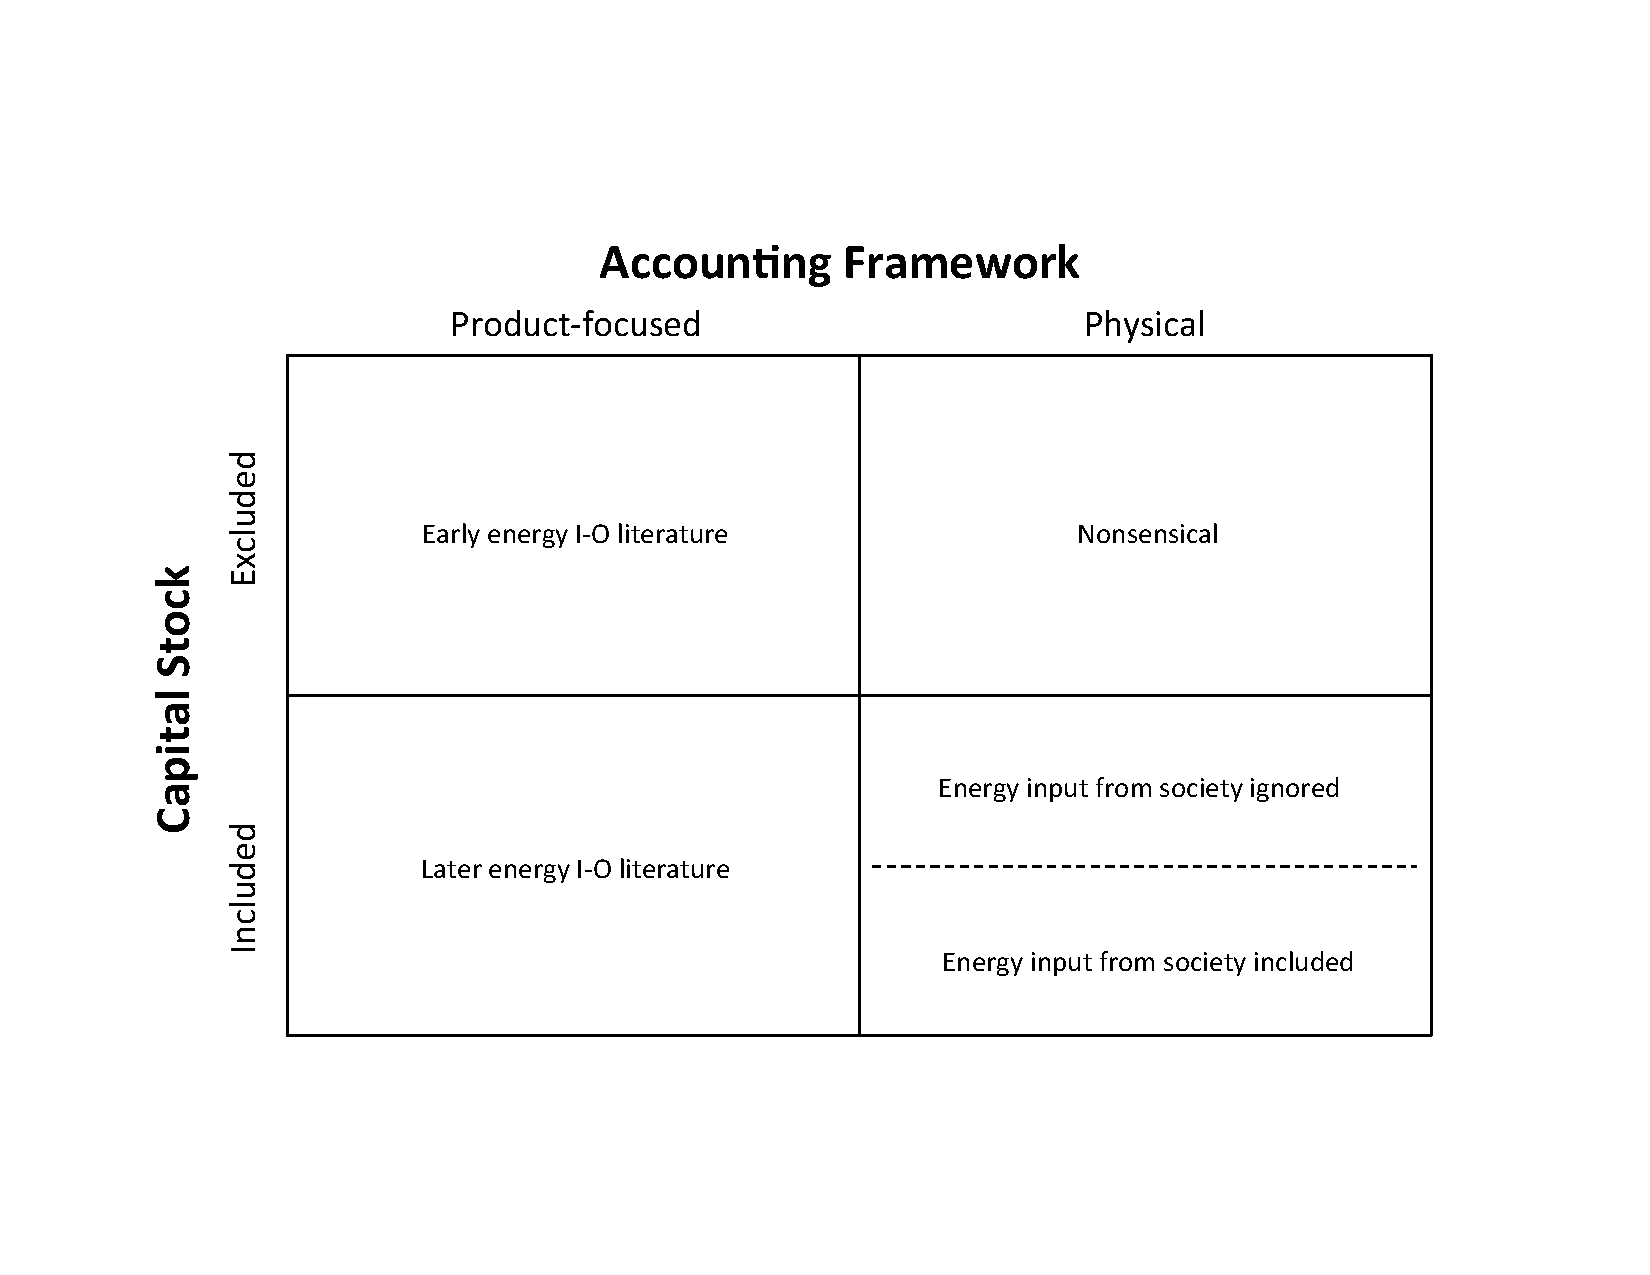
\includegraphics[width=0.8\linewidth]{Part_3/Chapter_Implications/Images/Grid.pdf}
\caption[Coordinates of analysis for implications for the I-O method]{Coordinates of analysis for implications for the EI-O method.}
\label{fig:coords_of_analysis}
\end{figure}


%+++++++++ I-O implications: product-based vs. physical ++++++++++
\subsection{Product-based vs.\ physical approaches}
\label{sec:prod_vs_physical}
%+++++++++

The distinction between product-focused and physical
accounting frameworks is located in the columns
of Figure~\ref{fig:coords_of_analysis}.
A \emph{physical accounting} framework strictly follows materials 
through the economy. 
Embodied energy is allocated to the material stock or material flow
in which it resides---wherever it goes, so goes the embodied energy. 
When the material is scrapped, so is its embodied energy.
For example, energy embodied within wastes ($\vec{B}_{waste}$) 
is not assigned to economic products. 
Rather, the energy embodied in wastes flows out of sectors 
into the biosphere \emph{with the waste material}.
In contrast, a \emph{product-focused accounting} framework assigns 
energy embodied in wastes to the products of the sector.
Both product-based and physical accounting frameworks
assign direct energy ($\dot{E}$) consumed by each sector
to the products of each sector.

Equation~\ref{eq:B_prod_physical_excluding_K} below
describes the outflow of embodied energy from sector $j$, 
for a physical accounting system 
that neglects both capital stock accumulation
and capital inflow (upper-right quadrant of
Figure~\ref{fig:coords_of_analysis}).\footnote{Equation~\ref{eq:B_prod_physical_excluding_K} 
	is used for illustrative purposes only. 
	A physical accounting framework would necessarily 
	include both flows and stocks of capital.
	Thus, the upper-right quadrant of Figure~\ref{fig:coords_of_analysis}
	(physical accounting framework that neglects capital)
	is labeled as nonsensical.}

\begin{equation} \label{eq:B_prod_physical_excluding_K}
	\dot{B}_{j}^{'}
	= \sum\limits_{i=1}^{n} \dot{B}_{ij}^{'} 
	- \dot{B}_{waste,j}
	+ \dot{Q}_{j0}
\end{equation}

\noindent{}Terms written with a ``prime''
(e.g.~$\dot{B}_{j}^{'}$) indicate definitions and terms that 
exclude input capital flows~($\dot{K}$) and capital stock~($K$).
The term~$\dot{B}_{waste,j}$ represents the energy embodied 
within wasted resource~($\dot{R}_{j0}$) 
and short-lived~($\dot{S}_{j0}$) material flows.
The $\dot{B}_{waste,j}$ term is subtracted, because waste material flows \emph{out of}
the sector. 
In a physical accounting framework, the energy embodied 
in waste flows ($\dot{B}_{waste,j}$)
is not assigned to the product~($\dot{B}_{j}^{'}$).

In contrast, Equation~\ref{eq:B_prod_product_excluding_K} describes the outflow 
of embodied energy from sector~$j$,
exclusive of capital stock,
for a product-focused accounting framework 
(upper left quadrant of Figure~\ref{fig:coords_of_analysis}).

\begin{equation} \label{eq:B_prod_product_excluding_K}
	\dot{B}_{j}^{'}
	= \sum\limits_{i=1}^{n} \dot{B}_{ij}^{'} 
	+ \dot{Q}_{j0}
\end{equation}

\noindent{}Notice that Equation~\ref{eq:B_prod_product_excluding_K} 
does not subtract the energy embodied in waste resource and short-lived material
flows ($\dot{B}_{waste,j}$) on the right side of the equation, 
because product-focused accounting systems assign energy embodied in wastes
to products.


%+++++++++ I-O implications: Capital stock ++++++++++
\subsection{Capital flows and stock}
\label{sec:capital_stock}
%+++++++++

The rows of Figure~\ref{fig:coords_of_analysis}
represent the role of capital flows and stock in an accounting framework.
The BEA Industry Accounts 
include capital flows in the ``make''
tables for each industry~\cite[Table~1]{Streitwieser:2011aa}, 
but capital inflows are accounted separately 
from intermediate uses as 
``Private fixed invest­ment''~\cite[Table~2]{Streitwieser:2011aa}.
During the earliest years of the EI-O method 
(prior to the mid-1970s) 
both capital inflows to economic sectors 
and stocks of capital were ignored.
In essence, the state of the art was located in the upper-left quadrant
of Figure~\ref{fig:coords_of_analysis}.
In time, Kirkpatrick~\cite{Kirkpatrick:1974te}, 
Bullard and Herendeen~\cite{Bullard-III:1975aa},
and Casler~\cite{Casler:1983uy} attempted to 
include inflows of capital in a product-focused
accounting framework, thereby moving the state of the art 
to the lower-left quadrant of Figure~\ref{fig:coords_of_analysis}.

We agree with this move, because of the many ways in which
capital stock is important for economies.
We can use the work of Eugene Odum~\cite{Odum1969}
to explain the importance of capital stock
within ecosystems,
and we have Herman Daly to thank
for making the connection between
ecosystems and economies.\cite{Daly1995}

In 1969, Odum outlined a number of 
defining characteristics of both \emph{developmental}
(growing) and \emph{mature} (stable) ecosystems in terms of key
properties of the system.\cite{Odum1969}
Ecosystems cannot
grow indefinitely in their (photosynthetic)~production rate~($P$)
due to the necessity of increasing maintenance
demands as the stock of biomass~($B$) increases.
Eventually, all production is used in this manner
and growth ceases 
$\left(\frac{\mathrm{d}}{\mathrm{d}t}(P) = 0\right)$.

In the early stages of ecosystem development,
the energy production rate 
per unit of biomass stock~$\left( \frac{P}{B} \right)$
is high.
As the ecosystem approaches maturity,
this ratio decreases.
Put another way,
the biomass stock (maintained) per unit of energy produced
$\left( \mathrm{the \; inverse \; ratio, \;} \frac{B}{P} \right)$
starts low and asymptotically increases to a maximum
when growth (in both $P$ and $B$) has ceased. 
The value of $\frac{B}{P}$ at the asymptote may be high or low\footnote{The
	value of $\frac{B}{P}$ at maturity (and the time taken to reach it)
	``may vary not only with different climatic 
	and physiographic situations but also with
	different ecosystem attributes in the same physical 
	environment.''~\cite[p.263]{Odum1969}}
and may therefore be considered a measure of 
the ``efficiency'' to which the ecosystem applies
energy production toward
the goal of maintaining biomass stock.
 
Turning back to economies,
Daly has, in our view,
correctly applied this concept to societal patterns
of economic consumption.\cite{Daly1995}
Our framework analogously suggests that
as capital stock~($\vec{B}_{K}$) increases,
an increasing flow of energy supply~($\vec{E}_{0}$)
will be needed to maintain that stock.\footnote{Today's economies 
	(and economic models and economic assumptions) are still focused
	on the objective of growth.
	If energy supply rates ($\vec{E}_{0}$) are constrained,
	these dynamics provide a possible reason for the difficulty
	of maintaining high levels of economic growth
	in mature economies.
	Eventually,
	we must learn to maximize the $\frac{B}{P}$
	ratios of our economies 
	$\left(\frac{\vec{B}_{K}}{\vec{E}_{0}}\right)$.}
Thus, it is important to account for capital stock in 
a material, energy, and value accounting framework.

To see the effect of the move from the upper-left to the lower-left
quadrant of Figure~\ref{fig:coords_of_analysis}, 
it is important to understand clearly both the assumptions and data that were used.
Energy analysts in the mid-1970s were utilizing the BEA
I-O tables,
which include capital flows on the output, but do not include capital flows on the input. 
Thus, this early literature implicitly assumes that 

\begin{equation} \label{eq:a_prime_lit}
	a_{ij}^{'} 
	\equiv \frac{\dot{X}_{\dot{R}_{ij}} + \dot{X}_{\dot{S}_{ij}}}
				{\dot{X}_{\dot{R}_{j}} + \dot{X}_{\dot{S}_{j}} + \dot{X}_{\dot{K}_{j}}}
	= \frac{\dot{X}_{ij}^{'}}{\dot{X}_{j}}.
\end{equation}

\noindent{}Comparison between Equations~\ref{eq:aij_def_expanded}
and~\ref{eq:a_prime_lit}
highlights the fact that the early literature neglects flows of capital stock
($\dot{X}_{\dot{K}_{ij}}$) on the input.
Thus, the Input-Output matrix in the early EI-O literature
($\vec{A^{'}}$) is

\begin{equation} \label{eq:A_matrix_def_literature}
	\vec{A}^{'} 
	=
	\begin{bmatrix}
		a_{22}^{'} & a_{23}^{'}	\\[4pt]   % [4pt] gives a little extra vertical space.
		a_{32}^{'} & a_{33}^{'}	
	\end{bmatrix}.
\end{equation}

% \noindent{}Furthermore, the early literature implicitly defines 
% energy intensity as
% 
% \begin{equation}
% 	\varepsilon_{j}^{'} 
% 	= \frac{\dot{T}_{j}^{'}}{\dot{X}_{j}^{'}},
% \end{equation}
% 
% \noindent{}with
% 
% \begin{equation}
% 	\dot{T}_{j}^{'} \equiv \dot{T}_{\dot{R}_{j}} + \dot{T}_{\dot{S}_{j}}
% \end{equation}
% 
% \noindent{}and
% 
% \begin{equation}
% 	\dot{X}_{j}^{'} \equiv \dot{X}_{\dot{R}_{j}} + \dot{X}_{\dot{S}_{j}}.
% \end{equation}
% 
% \noindent{}The above equations implicitly ignore both value and energy embodied within
% flows of capital.
% \noindent{}In contrast, our framework (Equation~\ref{eq:X_hat_matrix_def})
% includes capital flows explicitly:
% 
% \begin{equation}
% 	\hat{\vec{X}} = \hat{\vec{X}}_{\dot{R}} + \hat{\vec{X}}_{\dot{S}} + \hat{\vec{X}}_{\dot{K}}.
% \end{equation}
% 
The implicit assumptions of the early energy I-O literature 
are consistent with the upper-left quadrant
of Figure~\ref{fig:coords_of_analysis}, 
and the energy intensity equation
found in most of the early literature is

\begin{equation} \label{eq:intensity_upper_left}
	\boldsymbol{\varepsilon}^{'}
	= {\left( \vec{I} - {\vec{A}^{'}}^{\mathrm{T}} \right)}^{-1}
		{\left( \hat{\vec{X}} \right)}^{-1}
		\vec{E}_{0}.
\end{equation}

Bullard and Herendeen~\cite{Bullard-III:1975aa}, 
following Kirkpatrick~\cite{Kirkpatrick:1974te},
added flows of capital as inputs 
to each sector~\cite[Figure~5]{Bullard-III:1975aa},
and, in so doing, changed Equation~\ref{eq:intensity_upper_left}
to Equation~\ref{eq:intensity_lower_left}:

\begin{equation} \label{eq:intensity_lower_left}
	\boldsymbol{\varepsilon}
	= {\left[ \vec{I} - 
			\left( {\vec{A}^{'}}^{\mathrm{T}} 
					+ \vec{A}_{\dot{K}}^{\mathrm{T}} \right) \right]}^{-1}
		{\left( \hat{\vec{X}} \right)}^{-1}	\vec{E}_{0}
\end{equation}

\noindent{}with

\begin{equation}
	\vec{A}_{\dot{K}}
	\equiv
	\begin{bmatrix}
		a_{\dot{K}_{22}}	& a_{\dot{K}_{23}} \\
		a_{\dot{K}_{32}}    & a_{\dot{K}_{33}} \\
	\end{bmatrix}
\end{equation}

\noindent{}and

\begin{equation}
	a_{\dot{K}_{ij}}
	\equiv
	\frac{\dot{X}_{\dot{K}_{ij}}}{\dot{X}_{j}}.
\end{equation}

Bullard and Herendeen
counted embodied energy 
from incoming capital stock in $\vec{A}_{\dot{K}}$ 
only if it was used
for replacement.\cite[p.~488]{Bullard-III:1975aa}
Consequently, they did not count incoming energy embodied 
in capital if the incoming capital was used 
to increase the stock of capital within a sector.
In fact, Bullard and Herendeen's
product-focused accounting framework
did not include an embodied energy stock 
for economic sectors~($\vec{B}$) at all.
They assumed that half of the incoming capital 
went toward replacement.
These early researchers moved from the upper-left quadrant
to the lower-left quadrant of Figure~\ref{fig:coords_of_analysis}.
And, Equation~\ref{eq:intensity_lower_left} represents 
a partial step toward developing 
a method for estimating energy intensity ($\boldsymbol{\varepsilon}$)
that fully accounts for capital stock.

As stated above, we agree with Kirkpatrick~\cite{Kirkpatrick:1974te}, 
Bullard and Herendeen~\cite{Bullard-III:1975aa},
and Casler~\cite{Casler:1983uy} that incoming capital
is important and should be included in an accounting framework
(i.e., we should be on the lower half of Figure~\ref{fig:coords_of_analysis}).
But, we recommend that inclusion of incoming capital should
be done within a \emph{physical} accounting framework, 
i.e.\ we should make a second move from the lower-left to the lower-right
quadrant of Figure~\ref{fig:coords_of_analysis}.
Specifically, incoming capital should be included 
not only on incoming material streams but also
as a stock that can accumulate within the economic sector itself.

Our recommendation is informed by the work of 
Odum~\cite{Odum1969} and Daly~\cite{Daly1995}
and is based on the belief that
accounting for stocks of capital is important for developing a coherent view
of the structure of an economy. 
Stocks of capital are essential to the production process:
without machines and factories, cars cannot be produced. 
And, in industrialized economies 
maintenance of captial stock becomes an important 
driver of demand.
Thus, the buildup of capital stock (and associated embodied energy) 
within economic sectors is an essential aspect of industrialization.
Carefully tracking (on a physical, as opposed to financial, basis) 
capital stock in each economic sector is essential 
for understanding the network effects of 
upstream energy demand as new industries and products arise 
(e.g., electric vehicles). 

In a physical accounting system that includes capital stock
(lower-right quadrant of Figure~\ref{fig:coords_of_analysis}), 
energy embodied within accumulated capital stock
is not assigned to products ($\vec{P}$); 
rather, accumulated embodied energy is assigned to a stock of embodied energy
for each sector ($\vec{B}_{K}$).
And, the stock of embodied energy ($\vec{B}_{K}$)
can depreciate.

A physical accounting framework that fully includes capital stock
(lower-right quadrant of Figure~\ref{fig:coords_of_analysis}) 
is described by Equation~\ref{eq:intensity_lower_right_no_society}. 

\begin{equation} \label{eq:intensity_lower_right_no_society}
	\boldsymbol{\varepsilon}
	= {\left( \vec{I} - {\vec{A}}^{\mathrm{T}} \right)}^{-1}
		{\left( \hat{\vec{X}}  \right)}^{-1}
		\left[ \vec{E}_{0}
			  - \frac{\mathrm{d}\vec{B}_{K}}{\mathrm{d}t}
			  - \vec{B}_{waste}
			  - \hat{\boldsymbol{\gamma}}_{B} \vec{B}_{K} \right].
\end{equation}

\noindent{}Differences between Equation~\ref{eq:intensity_lower_right_no_society}
and Equation~\ref{eq:intensity_lower_left} include:

\begin{itemize}
	\item{Equation~\ref{eq:intensity_lower_right_no_society} includes $\vec{A}$
	while Equation~\ref{eq:intensity_lower_left} splits $\vec{A}$ into
	$\vec{A}^{'}$ and $\vec{A}_{\dot{K}}$ (a difference in appearance only),}
	
	\item{Equation~\ref{eq:intensity_lower_right_no_society} subtracts
	accumulation $\left( \frac{\mathrm{d}\vec{B}_{K}}{\mathrm{d}t} \right)$
	of energy embodied in capital stock,
	because energy embodied in the stock of capital 
	for a sector ($B_{K_{j}}$)
	is assigned to products of the sector,}
	
	\item{Equation~\ref{eq:intensity_lower_right_no_society} subtracts
	waste ($\vec{B}_{waste}$),
	because energy embodied in waste products is not assigned to 
	products of the sector, and}

	\item{Equation~\ref{eq:intensity_lower_right_no_society} subtracts
	depreciation ($\hat{\boldsymbol{\gamma}}_{B} \vec{B}_{K}$)
	of energy embodied in capital stock,
	because energy embodied in depreciated capital ($\dot{B}_{\dot{K}_{j0}}$)
	is assigned to products of the sector.}
\end{itemize}

There are two topics related to Equation~\ref{eq:intensity_lower_right_no_society} 
that are worthy of consideration:
waste flows and an accounting equation for capital stock.


%--------- I-O implications: Capital stock: Waste ----------
\subsubsection{Waste flows}
\label{sec:waste_flows}
%---------

We are unaware of any estimates of the energy embodied in wasted
material in an economy ($\vec{B}_{waste}$).  
But, it may be possible to develop a metric for the resource material efficiency of an 
economic sector ($\eta_{\dot{R}}$),
i.e.\ the fraction of the material that actually makes it into the product, 
such that:

\begin{equation} \label{eq:manufacturing_effiency}
	\eta_{\dot{R}_{j}}
	\equiv \frac{\dot{P}_{j}}{\sum\limits_{i=1}^{n} \dot{R}_{ij}}.
\end{equation}

\noindent{}With the above definition, 
the scrap rate for resources could be expressed as
$(1~-~\eta_{\dot{R}}) \sum\limits_{i=1}^{n} \dot{R}_{ij}$.
Allwood et.\ al.~\cite[p. 193]{allwood2012sustainable} 
used a process-based approach to manufacturing efficiencies
for metals used in manufacturing. 
The data are summarized in Table~\ref{tab:scrap_rates}.

\begin{table}
\caption[Manufacturing efficiencies for selected goods]{Manufacturing efficiencies
($\eta_{\dot{R}}$, 
Equation~\ref{eq:manufacturing_effiency})
for selected manufactured goods.\cite{allwood2012sustainable}}
\begin{center}
\begin{tabular} {r @{\hspace{2em}} l}
	\toprule
	Product & $\eta_{\dot{R}}$ [\%] \\
	\midrule
	Steel I-beam             & 90 \\
	Car Door Panel           & 50 \\
	Aluminium Drink Can      & 50 \\
	Aircraft Wing Skin Panel & 10 \\
	\bottomrule
\end{tabular}
\end{center}
\label{tab:scrap_rates}
\end{table}

Furthermore, one could assume that the rate
of short-lived materials ($\dot{S}$) used by a sector could be given as a 
fraction of the resource ($\dot{R}$) use rate such that:

\begin{equation}
	\rho_{\dot{S}_{j}}
	\equiv \frac{\dot{S}_{j0}}{\sum\limits_{i=1}^{n} \dot{R}_{ij}}
	= \frac{\sum\limits_{i=1}^{n} \dot{S}_{ij}}{\sum\limits_{i=1}^{n} \dot{R}_{ij}}.
\end{equation}

With the above definitions, the waste resource rate from an economic sector
can be given as

\begin{equation}
	\dot{R}_{j0} + \dot{S}_{j0}
	= (1 - \eta_{\dot{R}_{j}} + \rho_{\dot{S}_{j}}) \sum\limits_{i=1}^{n} \dot{R}_{ij}.
\end{equation}

\noindent{}The embodied energy in the waste materials would need to be estimated
from the embodied energy of the incoming resource and short-lived material flows as

\begin{equation}
	\dot{B}_{waste,j}
	= \dot{B}_{\dot{R}_{j0}} + \dot{B}_{\dot{S}_{j0}}.
\end{equation}


%--------- I-O implications: Capital stock: capital accounting equation ----------
\subsubsection{Simplification via capital stock accounting equation}
\label{sec:capital_accounting}
%---------

A possible simplification to Equation~\ref{eq:intensity_lower_right_no_society}
can be obtained from a control volume around the stock of capital in sector $j$:

\begin{equation}
	\frac{\mathrm{d}B_{K_{j}}}{\mathrm{d}t}
	= \sum\limits_{i=1}^{n} \dot{B}_{\dot{K}_{ij}} 
	- \gamma_{B_{j}} B_{K_{j}}.
\end{equation}

We can express the incoming energy embodied in capital ($\sum_{i=1}^{n} \dot{B}_{\dot{K}_{ij}}$)
as a fraction ($\alpha_{B_{j}}$) of the capital stock ($B_{K_{j}}$) as

\begin{equation}
	\alpha_{B_{j}}
	\equiv 
	\frac{\sum\limits_{i=1}^{n} \dot{B}_{\dot{K}_{ij}}} {B_{K_{j}}}
\end{equation}

\noindent{}for $j \in [2,n]$.

\noindent{}Together with the Kronecker delta ($\delta_{ij}$), we can write

\begin{equation}
	\hat{\boldsymbol{\alpha}}_{B}
	\equiv
	\delta_{ij} \alpha_{B_{j}}
	=
	\begin{bmatrix}
		\alpha_{B_{2}}	& 0               \\
		0               & \alpha_{B_{3}}  \\
	\end{bmatrix}.
\end{equation}

\noindent{}Thus, the embodied energy accounting equation around
the stock of capital in the economy can be written in matrix form as

\begin{equation}
	\frac{\mathrm{d}\vec{B}_{K}}{\mathrm{d}t}
	= \hat{\boldsymbol{\alpha}}_{B} \vec{B}_{K}
	- \hat{\boldsymbol{\gamma}}_{B} \vec{B}_{K}.
\end{equation}

\noindent{}Rearranging slightly gives

\begin{equation} \label{eq:alpha_cap_stock}
	\hat{\boldsymbol{\alpha}}_{B} \vec{B}_{K}
	= \frac{\mathrm{d}\vec{B}_{K}}{\mathrm{d}t}
	+ \hat{\boldsymbol{\gamma}}_{B} \vec{B}_{K},
\end{equation}

\noindent{}which says that incoming capital ($\hat{\boldsymbol{\alpha}}_{B} \vec{B}_{K}$)
can be used to either
increase the stock of capital in the economy 
$\left( \frac{\mathrm{d}\vec{B}_{K}}{\mathrm{d}t} \right)$
or overcome depreciation ($\hat{\boldsymbol{\gamma}}_{B} \vec{B}_{K}$).
Substituting Equation~\ref{eq:alpha_cap_stock} into
Equation~\ref{eq:intensity_lower_right_no_society} gives

\begin{equation} \label{eq:epsilon_leontief_with_A_alpha}
	\boldsymbol{\varepsilon} 
	= {(\vec{I} - \vec{A}^{\mathrm{T}})}^{-1}\hat{\vec{X}}^{-1}
		\left[\vec{E}_{0} 
				- \hat{\boldsymbol{\alpha}}_{B} \vec{B}_{K}
				- \vec{B}_{waste}
		\right].
\end{equation}


%+++++++++ I-O implications: Energy input from society ++++++++++
\subsection{Energy input from society}
\label{sec:energy_from_society}
%+++++++++

In Sections~\ref{sec:prod_vs_physical}
and~\ref{sec:capital_stock} above,
we implicitly assumed that society 
(final consumption, Sector~1 in our example economies A--C) % chktex 8
contributes negligible energy to the economy.
Thus, all vectors and matrices in Equation~\ref{eq:intensity_lower_right_no_society}
involve Sectors~2--$n$, but not Sector~1.

Energy input from society to the economy ($\vec{T}_{1}$)
is ``muscle work'' supplied by working humans 
and draft animals.\cite{Ayres:2003ec,Ayres:2010ug,Warr:2012cg} 
This muscle work term ($\vec{T}_{1}$) should include
all upstream energy required to make the labor available.\footnote{At this point 
	in the development of our framework,
	we are assuming that Final Consumption (Sector 1) is exogenous to the economy 
	(Sectors 2\ldots{}$n$), 
	and upstream energy consumption needs to be included manually.
	However, in Section~\ref{sec:what_is_endogenous}, we show that Final Consumption
	can be endogenized.
	Once endogenized, the energy intensity of Final Consumption ($\varepsilon_{1}$) 
	will automatically include the upstream energy required to make labor available.
	(See Appendix~\ref{chap:infinite_series}.)

	It is important to note, too, that labor can have very high energy intensity, 
	because $\varepsilon_{1}$ includes the energy required to supply food 
	for and transport to workers.} 
Equation~\ref{eq:epsilon_leontief_with_A} 
adds the effect of energy input from society to the economy,
effectively moving from the top half to the lower half of the lower-right quadrant
in Figure~\ref{fig:coords_of_analysis}.

\begin{equation}
	\boldsymbol{\varepsilon} 
	= {(\vec{I} - \vec{A}^{\mathrm{T}})}^{-1}\hat{\vec{X}}^{-1}
		\left[\vec{E}_{0} 
				+ \vec{T}_{1} 
				- \frac{\mathrm{d}\vec{B}_{K}}{\mathrm{d}t} 
				- \vec{B}_{waste}
				- \hat{\boldsymbol{\gamma}}_{B}\vec{B}_{K}
		\right].\tag{\ref{eq:epsilon_leontief_with_A}}
\end{equation}

For industrialized economies, the direct energy component ($\vec{E}_{1}$) 
of muscle work ($\vec{T}_{1}$)
is likely to provide only a small fraction
of the energy input from fossil fuels ($\vec{E}_{0}$).
But, the embodied energy of the muscle work ($\vec{B}_{1}$) is likely to be large.
For agrarian
and developing economies, 
$\vec{T}_{1}$ and $\vec{E}_{0}$ 
could be on the same order of magnitude.
For both industrial and agrarian economies,
neglecting $\vec{T}_{1}$ could cause errors
in estimates of $\boldsymbol{\varepsilon}$.
To the extent that $\vec{T}_{1}$ 
is significant relative to $\vec{E}_{0}$,
neglecting $\vec{T}_{1}$
will underpredict the energy intensity of economic output.
Energy input from society is discussed further 
in Section~\ref{sec:what_is_endogenous}.


%+++++++++ I-O implications: Recommendation ++++++++++
\subsection{Recommendation}
\label{sec:I-O_recommendation}
%+++++++++

Sections~\ref{sec:prod_vs_physical}--\ref{sec:energy_from_society} 
discussed three factors that affect the form of the
energy intensity equation: 
product-focused vs.\ physical accounting frameworks,
whether capital stock is included, and
whether energy input from society is included.
The three factors are summarized in Figure~\ref{fig:coords_of_analysis}.

At this point, it is instructive to look back at the 
product-focused vs.\ physical discussion in Section~\ref{sec:prod_vs_physical}.
We understand the argument for including capital stock in a product-focused
accounting framework (lower-left quadrant of Figure~\ref{fig:coords_of_analysis}):
capital stock and waste exist 
solely due to product demand, 
therefore energy embodied in capital and waste should be assigned to products. 
However, a product-focused framework that includes capital stock (lower-left quadrant of
Figure~\ref{fig:coords_of_analysis})
masks structural aspects of economies
that we believe are essential to fully understanding how and why energy flows 
through economies, namely the accumulation of capital
and associated energy embodied within sectors.

The metabolic metaphor provides guidance here. 
If we were to create a model of an organism that neglects 
tissues that accumulate embodied energy,
the organism (in the model) has nothing with which to 
absorb, process, waste, or otherwise exchange
material with the biosphere.
The organism doesn't physically exist (in the model)!
Neglecting to account for the stock of capital (and its embodied energy) 
is tantamount to assuming that economic production occurs out of nothing!
Accounting for capital stock is essential.

For our framework, we chose a physical accounting approach
(which puts us in the right column of Figure~\ref{fig:coords_of_analysis}).
We chose the physical approach primarily because of our belief that 
capital is an important aspect of economies,
and the physical accounting framework
properly includes a stock of capital for each sector of the economy.
Product-based accounting frameworks mask crucial aspects 
of why and how energy flows through economies.
We acknowledge that the choice of a physical accounting framework necessitates
careful tracking of capital flows (and associated embodied energy)
through the economy. 
For more on data needs, see Section~\ref{sec:Data}.

Finally, we suggest that accounting for energy input from society
to the economy is important, 
and we need to be in the lower half of the bottom-right quadrant
of Figure~\ref{fig:coords_of_analysis}.
So, the state of the art has moved from the nascent energy I-O literature
located in the upper-left quadrant of Figure~\ref{fig:coords_of_analysis}
as represented by Equation~\ref{eq:intensity_upper_left}
through the lower-left quadrant of Figure~\ref{fig:coords_of_analysis}
as represented by Equation~\ref{eq:intensity_lower_left}
to the lower half of the bottom-right quadrant 
of Figure~\ref{fig:coords_of_analysis}
as represented by Equation~\ref{eq:epsilon_leontief_with_A}.

The implication of the detailed development of our framework
on the EI-O method is 
some suggested enhancements to the EI-O method, 
including

\begin{itemize}
	\item{conversion to a physical accounting framework such as the one we propose herein,}
	
	\item{physical (as opposed to financial) tracking 
	of accumulated capital stock within economic sectors,}
	
	\item{redefinition of $\vec{A}$ and $\boldsymbol{\varepsilon}$ to include
	embodied energy on inflows of material, and}
	
	\item{use of Equation~\ref{eq:epsilon_leontief_with_A} instead of
	Equations~\ref{eq:intensity_upper_left} or~\ref{eq:intensity_lower_left}
	for estimating energy intensity ($\boldsymbol{\varepsilon}$)
	of economic sectors within an economy.}
\end{itemize}
 

%%%%%%%%%% Implications %%%%%%%%%%
\section{Implications for economic growth}
\label{sec:implications_for_development}
%%%%%%%%%%

Across the world, economic health and well-being 
is measured almost exclusively 
by Gross Domestic Product (GDP). 
If GDP grows, the economy is said to be growing.\footnote{GDP 
	is not the only indicator of well-being available; 
	there are several other measures in use.
	The Human Development Index (HDI) is a globally accepted measure 
	that augments GDP with education and life expectancy.\cite{Malik:2013aa} 
	In the US, the state of Maryland has been tracking well-being 
	using the \emph{Genuine Progress Indicator} (MDGPI),
	which combines measures of economic transactions with 
	environmental and social costs.\cite{MDDNR:2013aa,Bagstad:2007aa} 
	The MDGPI is closely related to 
	Herman Daly's Index of Sustainable Economic Welfare (ISEW)
	which allows policy-makers to account for contributions of and impacts on 
	the natural environment.\cite{Daly:1994aa,MDDNR:2014ab}
	Another example is the Nation of Bhutan's \emph{Gross National Happiness} (GNH),
	a systematic, annual compliation 
		of survey and other data related to nine factors: 
		ecological diversity and resilience,
		psychological well-being,
		health,
		education, 
		culture, 
		time use, 
		good governance, 
		community vitality, and 
		living standards.\cite{Ura:2012aa,GNH:2014aa}
	These alternatives to GDP are slowly gaining acceptance, particularly
	as their valuation methods are strengthened.\cite{Lawn:2003aa}}
Our framework affords the opportunity to assess economic growth 
in several dimensions.
Viewing these dimensions through the lens of our framework 
illustrates some important points about measures 
of economic growth and well-being.

% We're not using this footnote, because we have moved 
% toward talking about ``growth'' and away from talking about ``development.''
% Economic ``development''\footnote{We choose 
% 	to use the word ``development'' to
% 	describe expanding economies, despite significant misgivings about the term. 
% 	The unambiguously positive connotations of the words ``development'' and ``developed''
% 	fail to capture the nuances of travel along economic development paths:
% 	there are so many ways in which life experience in ``developed'' countries 
% 	is both better and worse than life in ``developing'' countries.
% 	We hope to convey our misgivings by surrounding these words with quotation marks in this text.}
% 
With reference to Figure~\ref{fig:C_value}, GDP is calculated by

\begin{equation} \label{eq:GDP_def}
	GDP
	= \sum\limits_{j=2}^{n} \dot{X}_{j}
\end{equation}

\noindent{}where $n$ is the number of sectors in the economy.
Equation~\ref{eq:GDP_def} clearly shows that 
$GDP$ is a \emph{flow} of value in units of \$/year.

A second possible measure of economic well-being is a \emph{stock}, 
wealth:

\begin{equation} \label{eq:Dev_Integral_Wealth}
	X_{j}(t) 
	= X_{j}(0) 
	+ \int_{t=0}^{t=t} \frac{\mathrm{d}X_{j}}{\mathrm{d}t}\mathrm{d}t,
\end{equation}

\noindent{}where $j=1$ for societal wealth 
and $j \in [2,n]$ for corporate wealth, both measured in dollars.

As an economy grows,
sectors within the economy accumulate capital stock 
($K$, typically expressed in units of dollars)
and associated embodied energy 
($B_{K}$, expressed in units of joules).
If we turn this around, 
accumulation of embodied energy
in economic sectors and society 
could be considered a \emph{proxy} for growth.\footnote{Embodied energy 
	as a proxy for economic growth may be overly focused on capital stock, 
	therefore one-dimensional, and reductive, 
	but GDP and other measures are open to similar criticism.}
Equation~\ref{eq:Dev_Integral_Economy} indicates how accumulated
embodied energy in the capital stock 
of an economy ($\vec{B}_{K}$) could be calculated:

\begin{equation} \label{eq:Dev_Integral_Economy}
	\vec{B}_{K}(t) 
	= \vec{B}_{K}(0) 
	+ \int_{t=0}^{t=t} \frac{\mathrm{d}\vec{B}_{K}}{\mathrm{d}t}\mathrm{d}t,
\end{equation}

\noindent{}where $\vec{B}_{K}$ is given by Equation~\ref{eq:B_vec_def}.
Equation~\ref{eq:Dev_Integral_Economy} clearly shows
that energy embodied in capital ($\vec{B}_{K}$) 
is a \emph{stock} (in units of joules), not a flow.

The behavior of $\vec{B}_{K}$ 
with respect to
$\frac{\mathrm{d}\vec{B}_{K}}{\mathrm{d}t}$ 
is vitally important. 
As an economy transitions from agrarian to industrialized, 
its capital stock ($K$) and associated embodied energy ($B_{K}$)
grows ever larger. 
The outflow of depreciated capital stock and its associated embodied energy 
will occur at a faster rate, too.
As increasingly large amounts of energy are embodied 
in the capital stock of an economy ($B_{K}$), 
Equation~\ref{eq:matrix_leontief} shows that
increasingly large energy extraction rates ($\vec{E}_{0}$) 
are required to maintain capital stock 
in the sectors of the economy
to offset the effects of depreciation 
($\hat{\boldsymbol{\gamma}}_{B} \vec{B}_{K}$),
assuming that $\frac{\mathrm{d}\vec{B}_{K}}{\mathrm{d}t} \ge 0$ 
is desired. 

During a period of rapid industrialization and infrastructure build-out, 
we expect both GDP and energy embodied in the economy ($\vec{B}_{K}$)
to increase.
But, there is no guarantee that GDP and $\vec{B}_{K}$ move 
in the same direction at all times.
Industrialized economies may experience GDP growth while 
the stock of embodied energy in the economy ($\vec{B}_{K}$) remains nearly constant,
because the economy is running circles to overcome the effects of depreciation.

There can be a time lag between movements of GDP and $\vec{B}_{K}$, too.
At the beginning of an economic downturn (defined as prolonged GDP reduction),
capital stock and associated embodied energy ($\vec{B}_{K}$) will remain approximately constant:
GDP moves but $\vec{B}_{K}$ doesn't.
But as the GDP decline continues, 
maintenance flows for capital stock will be reduced.
If depreciation overtakes maintenance, $\vec{B}_{K}$ will decline. 

% This next paragraph is too speculative.
% We don't have evidence of this at this time.
% If economic decline is associated with significant external 
% infrastructure investment (such as occurred in post-colonial Africa),
% GDP may decrease 
% while the stock of energy embodied in the economy ($\vec{B}_{K}$) increases 
% due to foreign aid focused on infrastructure enhancement. 

``Extract and export'' economies may exhibit different dynamics.
GDP growth occurs as resources are extracted and sold, 
but $\vec{B}_{K}$ remains flat if that income is not 
invested back into the economy as capital. 
An example of this occured with rubber exports from the Amazon.
Per capita incomes increased by an order of magnitude 
from 1820 to 1900 during the rubber export boom. 
However, as Amazon rubber exports dropped in value
due to stiff competition from Asian rubber production, 
per capita incomes dropped precipitously back to original levels. 
Throughout this period, the capital stock, 
and presumably the stock of embodied energy ($\vec{B}_{K}$), 
remained nearly constant.\cite{bunker1984modes}

In fact, capital (represented by energy embodied in infrastructure, $\vec{B}_{K}$) and 
financial resources or wealth (represented by $X_{2 \ldots n}$) 
are complementary factors of production for economic processes. 
But, we can go further than linking physical capital with financial resources.
If capital~($\vec{B}_{K}$) is to be useful, we need financial resources
or currency~($\dot{X}$) to 
\begin{itemize}
	\item{purchase direct energy~($\dot{E}$) to power the capital,}
	
	\item{purchase resources~($\dot{R}$) to feed the capital, and}
	
	\item{pay workers~(represented 
	by societal energy input to the economy,~$\vec{T}_{1}$) 
	to operate the capital.}
\end{itemize}

Thus, economic growth could be considered a ``fully coupled'' problem:
understanding it requires breadth of knowledge and appreciation for 
interactions among many important factors.
Each factor discussed above 
($\dot{X}$, $X$, $\vec{B}_{K}$, $\dot{E}$, $\dot{R}$, and $\vec{T}_{1}$)
is necessary, but not sufficient, for economic growth.

Our framework serves to highlight several issues in economic growth. 
Should it be measured by a stock or a flow? 
Which measure is most appropriate? 
What roles do currency, capital stock, energy, resources, and labor
play in economic processes?
These are overlapping and complementary areas of inquiry, and
we encourage further research in all of these areas.


%%%%%%%%%% Implications %%%%%%%%%%
\section{Implications for recycling, reuse, and dematerialization}
\label{sec:recycling}
%%%%%%%%%%

Dematerialization is the idea that economic activity can be unlinked 
from material or energy demands.\cite{FischerKowalski:2011uo} 
One method for dematerializing an economy 
is reuse and recycling of materials from both
short-lived goods
$\left(\vec{B}_{waste}\right)$
and depreciated
capital stock~$\left(\hat{\boldsymbol{\gamma}}_{B}\vec{B}_{K}\right)$
that would otherwise have
been discarded to the biosphere.\footnote{The 
other prevailing theory in the economics literature, that
dematerialization will occur as the economy substitutes away from production of material goods 
toward information and services, has been strongly challenged 
by ecological economists.\cite{Bartelmus:2003vi,parrinello2004service}}

In Chapter~\ref{chap:intensity},
we defined the rate of accumulation 
of embodied energy within the economy
$\left(\frac{\mathrm{d}\vec{B}_{K}}{\mathrm{d}t}\right)$
by the following equation:

\begin{equation}
	\frac{\mathrm{d}\vec{B}_{K}}{\mathrm{d}t} 
	= \vec{E}_{0}
	+ \vec{T}_{1}
	+ \hat{\vec{X}} (\vec{A}^{\mathrm{T}} - \vec{I})\boldsymbol{\varepsilon} 
	- \vec{B}_{waste}
	- \hat{\boldsymbol{\gamma}}_{B}\vec{B}_{K}\tag{\ref{eq:matrix_leontief}}
\end{equation}

One effect of recycling is to reduce the magnitude 
of the waste 
$\left(\vec{B}_{waste}\right)$
and depreciation 
$\left(\hat{\boldsymbol{\gamma}}_{B}\right)$ terms.
As can be seen in Equation~\ref{eq:matrix_leontief},
reducing both $\vec{B}_{waste}$ 
and~$\hat{\boldsymbol{\gamma}}_{B}$, 
puts \emph{upward} pressure on the accumulation of 
energy embodied in capital stock
$\left(\frac{\mathrm{d}\vec{B}_{K}}{\mathrm{d}t}\right)$,
all other things being equal.

Recycling has a mixed effect on energy demand ($\vec{E}_{0}$). 
Because recycled materials can displace newly-produced material 
in the economy and society, 
recycling will tend to reduce energy demand ($\vec{E}_{0}$). 
However, recycling processes require energy to operate, 
thereby putting upward pressure on energy demand ($\vec{E}_{0}$). 
If the energetic cost of recycling is lower than 
the energetic cost of obtaining virgin materials, 
as is the case for many metals
(e.g.\ aluminum~\cite{Chapman1975}), 
the result is a net reduction of energy demand 
from the biosphere ($\vec{E}_{0}$). 
Berry and Fels found that recycling of the material in automobiles
would result in energy reduction of 12,640 kW-hr per vehicle.\cite[p.~15]{Berry:1973vo}
Therefore recycling will put \emph{downward} pressure on 
the growth of embodied energy in the economy
$\left(\frac{\mathrm{d}\vec{B}_{K}}{\mathrm{d}t}\right)$,
via reduced $\vec{E}_{0}$, all other things being equal. 

If recycling produces a net reduction in energy demand ($\vec{E}_{0}$), 
% i.e.\ if the effect of displaced production dominates over the effect 
% of energy consumed in recycling processes, 
the upward pressure on growth 
$\left(\frac{\mathrm{d}\vec{B}_{K}}{\mathrm{d}t}\right)$ 
from decrease in depreciation 
$\left(\hat{\boldsymbol{\gamma}}_{B}\right)$ 
and waste ($\vec{B}_{waste}$)
and the downward pressure on growth 
from net reduction in energy demand 
$\left(\vec{E}_{0}\right)$ 
can offset each other.
Under those conditions, 
the accumulation rate of energy embodied
in capital stock
$\left(\frac{\mathrm{d}\vec{B}_{K}}{\mathrm{d}t}\right)$ 
will remain near zero 
and total embodied energy 
$(\vec{B}_{K})$ will remain constant. 
In that scenario, 
dematerialization can occur: 
reduced material and energy input ($\vec{E}_{0}$) 
can be accompanied by 
no change in
the growth of the economy
$\left(\frac{\mathrm{d}\vec{B}_{K}}{\mathrm{d}t}\right)$.
However,
as will be discussed in Section~\ref{sec:material_quality},
recycled materials can never entirely replace
the need for virgin materials.


%%%%%%%%%% Implications %%%%%%%%%%
\section{Comparison to a steady-state economy}
\label{sec:SSE}
%%%%%%%%%%

\begin{quotation}
	Growth means larger jaws and a bigger digestive tract 
	for more rapidly converting more resources into more waste, 
	in the service of unexamined and frequently destructive 
	individual wants.
	Development means better digestion of a non-growing throughput, 
	and more worthy and satisfying goals to which our life energies 
	could be devoted.\cite{Daly:2012aa}
\end{quotation}

As discussed in Chapter~\ref{chap:intro},
the human economy is a subset of the biosphere, 
a finite, non-growing system.
Thus, the human economy cannot physically grow indefinitely.
The concept of a non-growing or ``steady-state'' economy
has existed for centuries.

There are a number of different
conditions that may characterize a system as steady-state.
In thermodynamics,
steady state is characterized by unchanging system properties ($p$),
such that $\left(\frac{\textrm{d}p}{\textrm{d}t}\right) = 0$.
In ecological economics, a steady-state
economy has been defined as a constant rate
of material throughput that maintains the stock
of ecological capital and provides a qualitatively well-lived life 
for the population.\cite[p.~32]{Daly1997}  
This definition is consistent
with zero rate of accumulation of stock. 
Ecological capital is not drawn down, 
nor is manufactured capital quantifiably increased. 
Increases in living standards result from economic ``development,'' 
in which qualitative 
improvement in life occurs through increases 
in ``efficiency, technology, and ethics.''~\cite[p.~167]{Daly1997} 

Two other conditions that might define a steady-state
economy are constant GDP or constant population.
Our framework, can address the first three steady-state conditions
(constant capital stock, constant throughput, and constant GDP).
The fourth condition (constant population) could be
accommodated with some adaptation of the 
framework. 
The issue of human population as part of society's
capital stock is addressed in Section~\ref{sec:people_as_stock}.


%+++++++++++++++++++++++++++++++++++++++++++
%+++++++++ Constant capital stock ++++++++++
%+++++++++++++++++++++++++++++++++++++++++++
\subsection{Constant level of capital stock}

In Chapter~\ref{chap:materials}, 
we introduced Equation~\ref{eq:C_CV_all_b}:

\begin{align}\tag{\ref{eq:C_CV_all_b}}
	- \frac{\mathrm{d}R_{0}}{\mathrm{d}t}										&
	=\sum_{j}\frac{\mathrm{d}K_{j}}{\mathrm{d}t}
	+ \sum_{i,j}\dot{S}_{ij}
	+ \sum_{j}\gamma_{K_{j}}K_{j}.
\end{align}

\noindent{}which indicates that 
natural resources in the 
biosphere~$\left(- \frac{\mathrm{d}R_{0}}{\mathrm{d}t}\right)$
are depleted by the economy
for the purposes of:

\begin{itemize}
	\item{increasing man-made capital stocks
	within the economy~$\left(\frac{\mathrm{d}K_{j}}{\mathrm{d}t}\right)$,}
	\item{providing short-lived goods exchanged within the
	economy~$\left(\dot{S}_{ij}\right)$, and}
	\item{overcoming depreciation of man-made
	capital stocks~$\left(\gamma_{K_{j}}K_{j}\right)$.}
\end{itemize}

Assuming,
first,
that a steady-state economy exists when the level
of capital stock remains constant
$\left(\sum_{j}\frac{\mathrm{d}K_{j}}{\mathrm{d}t}=0\right)$,\footnote{Note
that the steady-state condition does not preclude expansion
of some sectors of the economy, provided that there is 
equal contraction elsewhere.}
we can see that Equation~\ref{eq:C_CV_all_b}
reduces to:

\begin{align}\label{eq:C_CV_all_c}
	- \frac{\mathrm{d}R_{0}}{\mathrm{d}t}										&
	= \sum_{i,j}\dot{S}_{ij}
	+ \sum_{j}\gamma_{K_{j}}K_{j}.
\end{align}

A number of interesting concepts may be understood via
Equation~\ref{eq:C_CV_all_c}. 
Firstly,
if our steady-state economy is to be supported
sustainably,
then withdrawal of natural resources from the biosphere
$\left(\frac{\mathrm{d}R_{0}}{\mathrm{d}t}\right)$
had better be at some rate lower than the biosphere
can replenish those stocks. 
In reality, 
$\frac{\mathrm{d}R_{0}}{\mathrm{d}t}$
is really the sum of many different resources
(flora and fauna, water) each of which will have
its own natural rate of regeneration.
As such, 
the sustainability criterion  is a vector of values,
one for each natural resource, 
all of which be met individually.

Secondly,
the steady state condition 
$\left(\sum_{j}\frac{\mathrm{d}K_{j}}{\mathrm{d}t}=0\right)$
says nothing about the transfer rates of short-lived goods 
within in the economy $\left(\sum_{i,j}\dot{S}_{ij}\right)$
or the depreciation of capital stock back to the biopshere
$\left(\sum_{j}\gamma_{K_{j}}K_{j}\right)$.
Equation~\ref{eq:C_CV_all_c} indicates that 
the higher the rates of these flows,
the greater the rate of depletion of
natural resources, and the more difficult it will be to
meet the sustainability condition 
(that the withdrawal rate of natural resources from the biosphere
is lower than the biosphere
replenishment rate).
Within industrial society,
the flow of short-lived goods 
(packaging,
paper products,
disposable tableware,
cutlery,
and napkins)
is large,
and, presumably, attaining a sustainable steady-state economy
will be difficult.
This definition of steady state 
$\left(\sum_{j}\frac{\mathrm{d}K_{j}}{\mathrm{d}t}=0\right)$
does not necessarily coincide with sustainability.

As discussed in Chapter~\ref{chap:materials},
the rate of depreciation ($\gamma_{K}$) is inversely
proportional to the average lifetime of capital stock---as
the average lifetime of capital stock decreases,
the rate of depreciation of capital stock increases which
increases the draw on natural resources (by Equation~\ref{eq:C_CV_all_c}).
It is likely that the average lifetime of capital stock has
decreased over the last century, 
due to a decrease in durability of capital stock
(the average table built today is not as durable as the average table
built in the early twentieth century)
and also due to increasing proportions of consumer electronics
with short lifetimes (cell phones, laptops, tablets).
Decreasing lifetime causes higher rates of flow for
replacement materials.
In the absence of extreme recycling of materials,
these large replacement flows place large demands on
natural resources.

Thirdly,
the maintenance flows necessary to overcome
depreciation
$\left(\sum_{j}\gamma_{K_{j}}K_{j}\right)$
are proportional to the magnitude of the capital
stock ($K_{j}$).
As such,
a larger stock of capital requires
greater draw on natural resources and is thus harder
to maintain within any sustainability constraint.
These points emphasize that constant capital stock
(or analogously constant population)
is not a sufficient condition for environmental sustainability.


%++++++++++++++++++++++++++++++++++++++++
%+++++++++ Constant throughput ++++++++++
%++++++++++++++++++++++++++++++++++++++++
\subsection{Constant material throughput}

Herman Daly has placed great emphasis on a steady-state
economy as having a constant rate of material throughput 
\cite{Daly1977, Daly1997}
which, as discussed above, should be below biophysical limits
if sustainability is to be achieved.
This is often referred to as the ``scale'' issue---how 
large is the (currently growing) human economy in relation
to the finite, non-growing biosphere of which it is a sub-system?
Growth of the human economy must either displace other natural
ecosystems (replacing old growth forest with cultivated crops)
or deplete natural capital stocks, be they 
renewable (fisheries) or 
non-renewable (fossil fuels).
As shown in Figure~\ref{fig:C_materials},
material throughput is composed of two distinct processes:
exchange of material \emph{from} the biosphere 
\emph{into} the economy (extraction)
and exchange of material \emph{from} the economy
\emph{into} biosphere (waste and depreciation).
We may characterize constant material throughput
as either constant rate of extraction, constant rate of
waste disposal, or both.
In the language of our framework, we could write:

\begin{align}\label{eq:const_throughput}
	\frac{\mathrm{d}}{\mathrm{d}t}\left(\dot{R}_{0}\right)		&
	= 0																							\\
	\frac{\mathrm{d}}{\mathrm{d}t}\left(\dot{S}_{0}\right)		&
	= 0																						\\
	\sum\limits_{i}
			\left[
				\frac{\mathrm{d}}{\mathrm{d}t}\left(\dot{R}_{i0}\right)
				+ \frac{\mathrm{d}}{\mathrm{d}t}\left(\dot{S}_{i0}\right)
				+ \frac{\mathrm{d}}{\mathrm{d}t}\left(\dot{K}_{i0}\right)
			\right]																			&
	= 0.
\end{align}

The above equations say nothing about the level 
of man-made capital stock ($K$)
or the flow rate of short-lived goods ($\dot{S}$).
Thus, within the constant throughput constraint,
increasingly effective use of materials could
theoretically allow increasing accumulation
of man-made capital~($K$) 
and increasing flow of short-lived goods ($\dot{S}_{ij}$)
as society learns to use resources better.
Eventually,
physical limits would entail that capital
stock could no longer be increased.
Presumably,
society would desire that the throughput of
materials would be within levels that could
be sustained by the biosphere,
both at the input side---natural 
resources extracted at rates lower
than natural regeneration rates---and 
at the output side---wastes emitted 
at rates below which
the biosphere can assimilate.


%++++++++++++++++++++++++++++++++++++++++
%+++++++++ Constant GDP ++++++++++
%++++++++++++++++++++++++++++++++++++++++
\subsection{Constant GDP}

Although one definition of a steady-state economy is
based upon constant levels of \emph{material} throughput,
it is possible to examine the implications of constraining the \emph{value} of 
GDP to be constant.\footnote{This is a theoretical exercise, 
	as Daly takes great pains to be clear that 
	the steady-state economy is materially-based. ``It is not
	to be thought of as `zero growth in GNP'.''~\cite[p. 32]{Daly1997}}
Within our framework,
a condition of constant GDP would be
characterized by the following equation:

\begin{equation}\label{eq:const_GDP}
	\frac{\mathrm{d}}{\mathrm{d}t}\left(GDP\right)
	=	\sum\limits_{j}\frac{\mathrm{d}}{\mathrm{d}t}\left(\dot{X}_{j}\right)
	= 0.
\end{equation}

Because,
under the subjective theory of value,
no value is attributed to the flow of materials
to or from the biosphere,
it is unclear what impact constant GDP would have
on capital stock ($K$)
or material throughput
(both extraction and waste disposal).
If we constrained $\dot{R}_{0}$ and
$\dot{S}_{0}$, 
it is likely that economic growth would 
decrease or even become zero or negative
$\left(\frac{\mathrm{d}}{\mathrm{d}t}\left(GDP\right) \leq 0\right)$.
It is conceivable that constraining
economic growth may act to constrain
material throughput,
though this is certainly not assured.

Although constraining GDP may not achieve the desired restraint on material throughput,
increasing GDP may not produce a desired increase 
in material well-being, either. 
This is particularly 
true for countries that have already achieved high levels of wealth.  
Many authors argue that increasing GDP
no longer guarantees increasing welfare~\cite{G-R1975a, Wackernagel1996,
Cobb1999, Daly2006, Costanza2014} 
for two main reasons:
\begin{itemize}
	\item firstly, that the costs of growth in GDP (e.g., externalities 
           and defensive expenditures) outweigh any benefit 
	that comes from increasing GDP;\@ and
	
	\item secondly, that increased GDP 
	increases relative income inequality,
	which decreases welfare for both rich and poor 
	alike.\cite{Daly2006}
\end{itemize}

Indeed, it may be the case that at the margin an increase 
in GDP produces more ``illth'' than ``wealth,'' 
resulting
in ``uneconomic'' growth.\cite[p. 42]{Daly2006} 
Uneconomic growth is much more likely 
to occur in a wealthy society than in a poor one, 
according to the law of diminishing returns.\footnote{Measuring
whether or not growth is ``economic'' cannot be done 
with traditional measures, such as GDP, since there is no
debit column in the ledger for GDP\@.
However, alternative metrics, such as ISEW or GPI, can perform such a function.}
Thus, a case could be made for constraining GDP growth in wealthy countries 
so that resources may be allocated to poorer countries
where growth in GDP is still likely to be ``economic.''~\cite{Daly2006}


%****** Mik: Finish this section. 
%In terms of what a SSE would look like in the I-O framework, 
%at first blush, I would think that dB/dt = 0 is one aspect.  
%Also, with no growth, inflow rates = depreciation rates.  
%The larger that B is for any society, the larger E must be (to overcome depreciation).  
%To minimize E, hyper-recycling is probably useful.  
%Those are at least a place to start. ******
%
%****** In our discussion, 
%we also addressed the attempts at SSE from point of view of society. 
%In order to achieve this goal \emph{without} recycling, 
%the goods and services sector should have to increase extraction to offset decreasing ore grade, 
%the energy sector should have to increase extraction of energy 
%to allow increasing extraction (unless efficiency could make up the gap: unlikely) 
%in which case the SSE would be violated from these two and from the POV of the earth.
%******


%%%%%%%%%% Implications Summary %%%%%%%%%%
\section{Summary}
\label{sec:summary_implications}
%%%%%%%%%%

In this chapter, we discussed several implications that arise from 
the detailed development of our dynamic framework for material,
energy, and value accounting.
The first implications are for the EI-O method itself. 
We recommend a physical accounting framework that fully
accounts for capital stock and energy input from society 
(normally assumed to not provide direct energy to the economy).
We then discussed implications for economic ``growth,''
namely that economic growth could be considered a ``fully coupled'' problem: 
understanding it requires breadth of knowledge 
and appreciation for interactions among many important factors,
including financial capital, physical capital and associated embodied energy,
direct energy, resources, and societal inputs.
Each, alone, is necessary, but not sufficient, for economic growth.
We discussed implications for recycling and reuse of materials
as well as the concept of dematerialziation.
Finally, we viewed the concept of a steady-state economy through
the lens of our framework.
We found that there are many potential definitions of a steady-state economy,
none of which are fully satisfying when compared against the ideal 
of sustainability.

In the next chapter, we point to some unfinished business.


\bibliographystyle{unsrt}
\bibliography{../../EROI_review_v3}


% Always give a unique label
% and use \ref{<label>} for cross-references
% and \cite{<label>} for bibliographic references
% use \sectionmark{}
% to alter or adjust the section heading in the running head
%% Instead of simply listing headings of different levels we recommend to let every heading be followed by at least a short passage of text. Furtheron please use the \LaTeX\ automatism for all your cross-references and citations.

%% Please note that the first line of text that follows a heading is not indented, whereas the first lines of all subsequent paragraphs are.

%% Use the standard \verb|equation| environment to typeset your equations, e.g.
%
%% \begin{equation}
%% a \times b = c\;,
%% \end{equation}
%
%% however, for multiline equations we recommend to use the \verb|eqnarray|
%% environment\footnote{In physics texts please activate the class option \texttt{vecphys} to depict your vectors in \textbf{\itshape boldface-italic} type - as is customary for a wide range of physical subjects.}.
%% \begin{eqnarray}
%% a \times b = c \nonumber\\
%% \vec{a} \cdot \vec{b}=\vec{c}
%% \label{eq:01}
%% \end{eqnarray}

%% \subsection{Subsection Heading}
%% \label{subsec:2}
%% Instead of simply listing headings of different levels we recommend to let every heading be followed by at least a short passage of text. Furtheron please use the \LaTeX\ automatism for all your cross-references\index{cross-references} and citations\index{citations} as has already been described in Sect.~\ref{sec:2}.

%% \begin{quotation}
%% Please do not use quotation marks when quoting texts! Simply use the \verb|quotation| environment -- it will automatically render Springer's preferred layout.
%% \end{quotation}


%% \subsubsection{Subsubsection Heading}
%% Instead of simply listing headings of different levels we recommend to let every heading be followed by at least a short passage of text. Furtheron please use the \LaTeX\ automatism for all your cross-references and citations as has already been described in Sect.~\ref{subsec:2}, see also Fig.~\ref{fig:1}\footnote{If you copy text passages, figures, or tables from other works, you must obtain \textit{permission} from the copyright holder (usually the original publisher). Please enclose the signed permission with the manucript. The sources\index{permission to print} must be acknowledged either in the captions, as footnotes or in a separate section of the book.}

%% Please note that the first line of text that follows a heading is not indented, whereas the first lines of all subsequent paragraphs are.

% For figures use
%
%% \begin{figure}[b]
%% \sidecaption
% Use the relevant command for your figure-insertion program
% to insert the figure file.
% For example, with the option graphics use
%% \includegraphics[scale=.65]{figure}
%
% If not, use
%\picplace{5cm}{2cm} % Give the correct figure height and width in cm
%
%% \caption{If the width of the figure is less than 7.8 cm use the \texttt{sidecapion} command to flush the caption on the left side of the page. If the figure is positioned at the top of the page, align the sidecaption with the top of the figure -- to achieve this you simply need to use the optional argument \texttt{[t]} with the \texttt{sidecaption} command}
%% \label{fig:1}       % Give a unique label
%% \end{figure}


%% \paragraph{Paragraph Heading} %
%% Instead of simply listing headings of different levels we recommend to let every heading be followed by at least a short passage of text. Furtheron please use the \LaTeX\ automatism for all your cross-references and citations as has already been described in Sect.~\ref{sec:2}.

%% Please note that the first line of text that follows a heading is not indented, whereas the first lines of all subsequent paragraphs are.

%% For typesetting numbered lists we recommend to use the \verb|enumerate| environment -- it will automatically render Springer's preferred layout.

%% \begin{enumerate}
%% \item{Livelihood and survival mobility are oftentimes coutcomes of uneven socioeconomic development.}
%% \begin{enumerate}
%% \item{Livelihood and survival mobility are oftentimes coutcomes of uneven socioeconomic development.}
%% \item{Livelihood and survival mobility are oftentimes coutcomes of uneven socioeconomic development.}
%% \end{enumerate}
%% \item{Livelihood and survival mobility are oftentimes coutcomes of uneven socioeconomic development.}
%% \end{enumerate}


%% \subparagraph{Subparagraph Heading} In order to avoid simply listing headings of different levels we recommend to let every heading be followed by at least a short passage of text. Use the \LaTeX\ automatism for all your cross-references and citations as has already been described in Sect.~\ref{sec:2}, see also Fig.~\ref{fig:2}.

%% Please note that the first line of text that follows a heading is not indented, whereas the first lines of all subsequent paragraphs are.

%% For unnumbered list we recommend to use the \verb|itemize| environment -- it will automatically render Springer's preferred layout.

%% \begin{itemize}
%% \item{Livelihood and survival mobility are oftentimes coutcomes of uneven socioeconomic development, cf. Table~\ref{tab:1}.}
%% \begin{itemize}
%% \item{Livelihood and survival mobility are oftentimes coutcomes of uneven socioeconomic development.}
%% \item{Livelihood and survival mobility are oftentimes coutcomes of uneven socioeconomic development.}
%% \end{itemize}
%% \item{Livelihood and survival mobility are oftentimes coutcomes of uneven socioeconomic development.}
%% \end{itemize}

%% \begin{figure}[t]
%% \sidecaption[t]
% Use the relevant command for your figure-insertion program
% to insert the figure file.
% For example, with the option graphics use
%% \includegraphics[scale=.65]{figure}
%
% If not, use
%\picplace{5cm}{2cm} % Give the correct figure height and width in cm
%
%% \caption{Please write your figure caption here}
%% \label{fig:2}       % Give a unique label
%% \end{figure}

%% \runinhead{Run-in Heading Boldface Version} Use the \LaTeX\ automatism for all your cross-references and citations as has already been described in Sect.~\ref{sec:2}.

%% \subruninhead{Run-in Heading Italic Version} Use the \LaTeX\ automatism for all your cross-refer\-ences and citations as has already been described in Sect.~\ref{sec:2}\index{paragraph}.
% Use the \index{} command to code your index words
%
% For tables use
%
%% \begin{table}
%% \caption{Please write your table caption here}
%% \label{tab:1}       % Give a unique label
%
% For LaTeX tables use
%
%% \begin{tabular}{p{2cm}p{2.4cm}p{2cm}p{4.9cm}}
%% \hline\noalign{\smallskip}
%% Classes & Subclass & Length & Action Mechanism  \\
%% \noalign{\smallskip}\svhline\noalign{\smallskip}
%% Translation & mRNA$^a$  & 22 (19--25) & Translation repression, mRNA cleavage\\
%% Translation & mRNA cleavage & 21 & mRNA cleavage\\
%% Translation & mRNA  & 21--22 & mRNA cleavage\\
%%Translation & mRNA  & 24--26 & Histone and DNA Modification\\
%%\noalign{\smallskip}\hline\noalign{\smallskip}
%%\end{tabular}
%%$^a$ Table foot note (with superscript)
%%\end{table}
%
%% \section{Section Heading}
%%\label{sec:3}
% Always give a unique label
% and use \ref{<label>} for cross-references
% and \cite{<label>} for bibliographic references
% use \sectionmark{}
% to alter or adjust the section heading in the running head
%% Instead of simply listing headings of different levels we recommend to let every heading be followed by at least a short passage of text. Furtheron please use the \LaTeX\ automatism for all your cross-references and citations as has already been described in Sect.~\ref{sec:2}.

%% Please note that the first line of text that follows a heading is not indented, whereas the first lines of all subsequent paragraphs are.

%%If you want to list definitions or the like we recommend to use the Springer-enhanced \verb|description| environment -- it will automatically render Springer's preferred layout.

%%\begin{description}[Type 1]
%%\item[Type 1]{That addresses central themes pertainng to migration, health, and disease. In Sect.~\ref{sec:1}, Wilson discusses the role of human migration in infectious disease distributions and patterns.}
%%\item[Type 2]{That addresses central themes pertainng to migration, health, and disease. In Sect.~\ref{subsec:2}, Wilson discusses the role of human migration in infectious disease distributions and patterns.}
%%\end{description}

%%\subsection{Subsection Heading} %
%% In order to avoid simply listing headings of different levels we recommend to let every heading be followed by at least a short passage of text. Use the \LaTeX\ automatism for all your cross-references and citations citations as has already been described in Sect.~\ref{sec:2}.

%% Please note that the first line of text that follows a heading is not indented, whereas the first lines of all subsequent paragraphs are.

%% \begin{svgraybox}
%% If you want to emphasize complete paragraphs of texts we recommend to use the newly defined Springer class option \verb|graybox| and the newly defined environment \verb|svgraybox|. This will produce a 15 percent screened box 'behind' your text.

%% If you want to emphasize complete paragraphs of texts we recommend to use the newly defined Springer class option and environment \verb|svgraybox|. This will produce a 15 percent screened box 'behind' your text.
%% \end{svgraybox}


%% \subsubsection{Subsubsection Heading}
%%Instead of simply listing headings of different levels we recommend to let every heading be followed by at least a short passage of text. Furtheron please use the \LaTeX\ automatism for all your cross-references and citations as has already been described in Sect.~\ref{sec:2}.

%% Please note that the first line of text that follows a heading is not indented, whereas the first lines of all subsequent paragraphs are.

%% \begin{theorem}
%% Theorem text goes here.
%% \end{theorem}
%
% or
%
%% \begin{definition}
%% Definition text goes here.
%% \end{definition}

%% \begin{proof}
%\smartqed
%% Proof text goes here.
%% \qed
%% \end{proof}

%%\paragraph{Paragraph Heading} %
%% Instead of simply listing headings of different levels we recommend to let every heading be followed by at least a short passage of text. Furtheron please use the \LaTeX\ automatism for all your cross-references and citations as has already been described in Sect.~\ref{sec:2}.

%% Note that the first line of text that follows a heading is not indented, whereas the first lines of all subsequent paragraphs are.
%
% For built-in environments use
%
%%\begin{theorem}
%%Theorem text goes here.
%%\end{theorem}
%
%%\begin{definition}
%%Definition text goes here.
%%\end{definition}
%
%%\begin{proof}
%%\smartqed
%% Proof text goes here.
%%\qed
%%\end{proof}
%
%% \begin{acknowledgement}
%% If you want to include acknowledgments of assistance and the like at the end of an individual chapter please use the \verb|acknowledgement| environment -- it will automatically render Springer's preferred layout.
%% \end{acknowledgement}
%
%% \section*{Appendix}
%% \addcontentsline{toc}{section}{Appendix}
%
%% When placed at the end of a chapter or contribution (as opposed to at the end of the book), the numbering of tables, figures, and equations in the appendix section continues on from that in the main text. Hence please \textit{do not} use the \verb|appendix| command when writing an appendix at the end of your chapter or contribution. If there is only one the appendix is designated ``Appendix'', or ``Appendix 1'', or ``Appendix 2'', etc. if there is more than one.

%% \begin{equation}
%% a \times b = c
%% \end{equation}
% Problems or Exercises should be sorted chapterwise
%% \section*{Problems}
%% \addcontentsline{toc}{section}{Problems}
%
% Use the following environment.
% Don't forget to label each problem;
% the label is needed for the solutions' environment
%% \begin{prob}
%% \label{prob1}
%% A given problem or Excercise is described here. The
%% problem is described here. The problem is described here.
%% \end{prob}

%% \begin{prob}
%% \label{prob2}
%% \textbf{Problem Heading}\\
%% (a) The first part of the problem is described here.\\
%% (b) The second part of the problem is described here.
%% \end{prob}




%%%%%%%%%%%%%%%%%%%%% chapter.tex %%%%%%%%%%%%%%%%%%%%%%%%%%%%%%%%%
%
% sample chapter
%
% Use this file as a template for your own input.
%
%%%%%%%%%%%%%%%%%%%%%%%% Springer-Verlag %%%%%%%%%%%%%%%%%%%%%%%%%%
%\motto{Use the template \emph{chapter.tex} to style the various elements of your chapter content.}
\chapter{Conceptual and theoretical issues}
\chaptermark{Issues}
\label{chap:issues} % Always give a unique label
% use \chaptermark{}
% to alter or adjust the chapter heading in the running head

\abstract*{[NEED TO ADD ABSTRACT HERE]}

%% \abstract{Each chapter should be preceded by an abstract (10--15 lines long) that summarizes the content. The abstract will appear \textit{online} at \url{www.SpringerLink.com} and be available with unrestricted access. This allows unregistered users to read the abstract as a teaser for the complete chapter. As a general rule the abstracts will not appear in the printed version of your book unless it is the style of your particular book or that of the series to which your book belongs.\newline\indent
%% Please use the 'starred' version of the new Springer \texttt{abstract} command for typesetting the text of the online abstracts (cf. source file of this chapter template \texttt{abstract}) and include them with the source files of your manuscript. Use the plain \texttt{abstract} command if the abstract is also to appear in the printed version of the book.}

%% Use the template \emph{chapter.tex} together with the Springer document class SVMono (monograph-type books) or SVMult (edited books) to style the various elements of your chapter content in the Springer layout.



%%%%%%%%%% Conceptual and Theoretical Issues %%%%%%%%%%
\section{Choice of Energy Input Vector}
%%%%%%%%%%

Consistent with traditional I-O methods, the derivation presented above counts energy at the point of inflow to the economy. That is, elements of the energy input vector to the economy ($\vec{E}$) are zero except for those sectors that receive energy directly from the Earth. With the traditional approach, energy input to energy sectors is non-zero, and energy input to non-energy sectors is zero. So, in the two-sector example C above, $\dot{E}_{14} = 0$ and $\dot{E}_{13} \neq 0$. 

Costanza (1984) suggests an alternative approach, namely to count energy input to the economy at the point of conversion to useful work. Theoretical justification for this direct energy conversion (DEC) approach comes from both thermodynamic and economic considerations. The thermodynamic justification derives from the purpose of energy consumption in an economy, namely to produce useful work. If energy flows \emph{through} a sector, it should not be counted ``against" that sector: only energy that is converted to useful work \emph{in} the sector should be counted against that sector.

The economic justification derives from the typical treatment of transportation sectors of the economy. ****** More here. See Costanza (1984) for the transportation analogy. ******

The DEC approach implicitly redefines energy intensity to be the required amount of fossil fuel energy to produce a unit of economic output. 

****** Equation redefining $\varepsilon$ here.

In the DEC approach, electricity consumption is converted to its fossil energy equivalent (coal) before being ``applied" to an economic sector. And, refined petroleum is converted to its fossil energy equivalent (crude) before being ``applied" to an economic sector.

****** The DEC option is akin to my idea of substituting the 1st Law into the total energy equation. Show this derivation after redefining $\varepsilon$ to be embodied energy per dollar, not total energy per dollar. So, there is a second implicit assumption going on with Costanza (1984), namely that we have a re-derivation of energy intensity. ******

****** Show that re-derivation results in only counting the energy burned by each sector (or the waste heat off of each sector). Costanza (1984) shows that distributing energy input at the point of consumption reduces the variance of energy intensity across all sectors of the economy. ******


%%%%%%%%%% Conceptual and Theoretical Issues %%%%%%%%%%
\section{What is Endogenous?}
%%%%%%%%%%

Are government and households endogenous? Costanza (1980) was the first to endogenize government and households, because households provide services to the economy (labor) in exchange for wages and government provides services to the economy in exchange for taxes, both of which require energy. Costanza (1980) showed that by including government and households as sectors in the economy, the variation of energy intensity is significantly reduced across all sectors of the economy. 


%%%%%%%%%% Conceptual and Theoretical Issues %%%%%%%%%%
\section{What About the Sun?}
%%%%%%%%%%

Costanza (1980) includes an option to consider the sun as an input to the economy, thereby significantly increasing the energy intensity of agricultural sectors and other sectors that depend upon agricultural outputs, however Costanza (1984) did not include the sun \cite{Costanza1980, Costanza1984}. Whether solar input to the economy should be considered is probably dependent upon the objectives of the analysis. In this framework we are primarily interested in the effects of declining energy resource quality in industrial economies, due to depletion of fossil fuels. As such, inclusion of solar flows is unnecessary. However, expanding the framework to include non-industrial or more agrarian societies would probably require accounting for these flows. Additionally, similar concerns might be raised in dealing with a society that is largely reliant on solar or wind energy.   [EARLIER FOOTNOTE ON INDUSTRIAL VS. NON-INDUSTRIAL ECONOMIES COULD BE BROUGHT IN HERE - MD]

There are a number of means by which solar flows can be accounted. Short-term solar flows could be accounted in the output of agricultural and forestry sectors, as well as some of the renewable energy producers, such as solar thermal and PV, wind, ocean thermal, hydro-power and biomass. This method does not account for longer-term flows of solar energy used to form fossil fuels. The \emph{emergy} accounting method puts all flows in terms of \emph{em}bodied en\emph{ergy} flows \cite{Odum1975, Odum1996}. The basic unit of measure is the \emph{em}joule which is often given in terms of flows of solar energy embodied in the energy (or material) - the solar emjoules - per unit of resource, abbreviated to seJ/J for energy resources, or seJ/g for materials. As such, even fossil fuels, e.g. coal, extracted from the earth have an embodied energy of around 67,000 seJ/J \cite{Brown2004}. 


\bibliography{EROI_review_v2}
\bibliographystyle{unsrt}


% Always give a unique label
% and use \ref{<label>} for cross-references
% and \cite{<label>} for bibliographic references
% use \sectionmark{}
% to alter or adjust the section heading in the running head
%% Instead of simply listing headings of different levels we recommend to let every heading be followed by at least a short passage of text. Furtheron please use the \LaTeX\ automatism for all your cross-references and citations.

%% Please note that the first line of text that follows a heading is not indented, whereas the first lines of all subsequent paragraphs are.

%% Use the standard \verb|equation| environment to typeset your equations, e.g.
%
%% \begin{equation}
%% a \times b = c\;,
%% \end{equation}
%
%% however, for multiline equations we recommend to use the \verb|eqnarray|
%% environment\footnote{In physics texts please activate the class option \texttt{vecphys} to depict your vectors in \textbf{\itshape boldface-italic} type - as is customary for a wide range of physical subjects.}.
%% \begin{eqnarray}
%% a \times b = c \nonumber\\
%% \vec{a} \cdot \vec{b}=\vec{c}
%% \label{eq:01}
%% \end{eqnarray}

%% \subsection{Subsection Heading}
%% \label{subsec:2}
%% Instead of simply listing headings of different levels we recommend to let every heading be followed by at least a short passage of text. Furtheron please use the \LaTeX\ automatism for all your cross-references\index{cross-references} and citations\index{citations} as has already been described in Sect.~\ref{sec:2}.

%% \begin{quotation}
%% Please do not use quotation marks when quoting texts! Simply use the \verb|quotation| environment -- it will automatically render Springer's preferred layout.
%% \end{quotation}


%% \subsubsection{Subsubsection Heading}
%% Instead of simply listing headings of different levels we recommend to let every heading be followed by at least a short passage of text. Furtheron please use the \LaTeX\ automatism for all your cross-references and citations as has already been described in Sect.~\ref{subsec:2}, see also Fig.~\ref{fig:1}\footnote{If you copy text passages, figures, or tables from other works, you must obtain \textit{permission} from the copyright holder (usually the original publisher). Please enclose the signed permission with the manucript. The sources\index{permission to print} must be acknowledged either in the captions, as footnotes or in a separate section of the book.}

%% Please note that the first line of text that follows a heading is not indented, whereas the first lines of all subsequent paragraphs are.

% For figures use
%
%% \begin{figure}[b]
%% \sidecaption
% Use the relevant command for your figure-insertion program
% to insert the figure file.
% For example, with the option graphics use
%% \includegraphics[scale=.65]{figure}
%
% If not, use
%\picplace{5cm}{2cm} % Give the correct figure height and width in cm
%
%% \caption{If the width of the figure is less than 7.8 cm use the \texttt{sidecapion} command to flush the caption on the left side of the page. If the figure is positioned at the top of the page, align the sidecaption with the top of the figure -- to achieve this you simply need to use the optional argument \texttt{[t]} with the \texttt{sidecaption} command}
%% \label{fig:1}       % Give a unique label
%% \end{figure}


%% \paragraph{Paragraph Heading} %
%% Instead of simply listing headings of different levels we recommend to let every heading be followed by at least a short passage of text. Furtheron please use the \LaTeX\ automatism for all your cross-references and citations as has already been described in Sect.~\ref{sec:2}.

%% Please note that the first line of text that follows a heading is not indented, whereas the first lines of all subsequent paragraphs are.

%% For typesetting numbered lists we recommend to use the \verb|enumerate| environment -- it will automatically render Springer's preferred layout.

%% \begin{enumerate}
%% \item{Livelihood and survival mobility are oftentimes coutcomes of uneven socioeconomic development.}
%% \begin{enumerate}
%% \item{Livelihood and survival mobility are oftentimes coutcomes of uneven socioeconomic development.}
%% \item{Livelihood and survival mobility are oftentimes coutcomes of uneven socioeconomic development.}
%% \end{enumerate}
%% \item{Livelihood and survival mobility are oftentimes coutcomes of uneven socioeconomic development.}
%% \end{enumerate}


%% \subparagraph{Subparagraph Heading} In order to avoid simply listing headings of different levels we recommend to let every heading be followed by at least a short passage of text. Use the \LaTeX\ automatism for all your cross-references and citations as has already been described in Sect.~\ref{sec:2}, see also Fig.~\ref{fig:2}.

%% Please note that the first line of text that follows a heading is not indented, whereas the first lines of all subsequent paragraphs are.

%% For unnumbered list we recommend to use the \verb|itemize| environment -- it will automatically render Springer's preferred layout.

%% \begin{itemize}
%% \item{Livelihood and survival mobility are oftentimes coutcomes of uneven socioeconomic development, cf. Table~\ref{tab:1}.}
%% \begin{itemize}
%% \item{Livelihood and survival mobility are oftentimes coutcomes of uneven socioeconomic development.}
%% \item{Livelihood and survival mobility are oftentimes coutcomes of uneven socioeconomic development.}
%% \end{itemize}
%% \item{Livelihood and survival mobility are oftentimes coutcomes of uneven socioeconomic development.}
%% \end{itemize}

%% \begin{figure}[t]
%% \sidecaption[t]
% Use the relevant command for your figure-insertion program
% to insert the figure file.
% For example, with the option graphics use
%% \includegraphics[scale=.65]{figure}
%
% If not, use
%\picplace{5cm}{2cm} % Give the correct figure height and width in cm
%
%% \caption{Please write your figure caption here}
%% \label{fig:2}       % Give a unique label
%% \end{figure}

%% \runinhead{Run-in Heading Boldface Version} Use the \LaTeX\ automatism for all your cross-references and citations as has already been described in Sect.~\ref{sec:2}.

%% \subruninhead{Run-in Heading Italic Version} Use the \LaTeX\ automatism for all your cross-refer\-ences and citations as has already been described in Sect.~\ref{sec:2}\index{paragraph}.
% Use the \index{} command to code your index words
%
% For tables use
%
%% \begin{table}
%% \caption{Please write your table caption here}
%% \label{tab:1}       % Give a unique label
%
% For LaTeX tables use
%
%% \begin{tabular}{p{2cm}p{2.4cm}p{2cm}p{4.9cm}}
%% \hline\noalign{\smallskip}
%% Classes & Subclass & Length & Action Mechanism  \\
%% \noalign{\smallskip}\svhline\noalign{\smallskip}
%% Translation & mRNA$^a$  & 22 (19--25) & Translation repression, mRNA cleavage\\
%% Translation & mRNA cleavage & 21 & mRNA cleavage\\
%% Translation & mRNA  & 21--22 & mRNA cleavage\\
%%Translation & mRNA  & 24--26 & Histone and DNA Modification\\
%%\noalign{\smallskip}\hline\noalign{\smallskip}
%%\end{tabular}
%%$^a$ Table foot note (with superscript)
%%\end{table}
%
%% \section{Section Heading}
%%\label{sec:3}
% Always give a unique label
% and use \ref{<label>} for cross-references
% and \cite{<label>} for bibliographic references
% use \sectionmark{}
% to alter or adjust the section heading in the running head
%% Instead of simply listing headings of different levels we recommend to let every heading be followed by at least a short passage of text. Furtheron please use the \LaTeX\ automatism for all your cross-references and citations as has already been described in Sect.~\ref{sec:2}.

%% Please note that the first line of text that follows a heading is not indented, whereas the first lines of all subsequent paragraphs are.

%%If you want to list definitions or the like we recommend to use the Springer-enhanced \verb|description| environment -- it will automatically render Springer's preferred layout.

%%\begin{description}[Type 1]
%%\item[Type 1]{That addresses central themes pertainng to migration, health, and disease. In Sect.~\ref{sec:1}, Wilson discusses the role of human migration in infectious disease distributions and patterns.}
%%\item[Type 2]{That addresses central themes pertainng to migration, health, and disease. In Sect.~\ref{subsec:2}, Wilson discusses the role of human migration in infectious disease distributions and patterns.}
%%\end{description}

%%\subsection{Subsection Heading} %
%% In order to avoid simply listing headings of different levels we recommend to let every heading be followed by at least a short passage of text. Use the \LaTeX\ automatism for all your cross-references and citations citations as has already been described in Sect.~\ref{sec:2}.

%% Please note that the first line of text that follows a heading is not indented, whereas the first lines of all subsequent paragraphs are.

%% \begin{svgraybox}
%% If you want to emphasize complete paragraphs of texts we recommend to use the newly defined Springer class option \verb|graybox| and the newly defined environment \verb|svgraybox|. This will produce a 15 percent screened box 'behind' your text.

%% If you want to emphasize complete paragraphs of texts we recommend to use the newly defined Springer class option and environment \verb|svgraybox|. This will produce a 15 percent screened box 'behind' your text.
%% \end{svgraybox}


%% \subsubsection{Subsubsection Heading}
%%Instead of simply listing headings of different levels we recommend to let every heading be followed by at least a short passage of text. Furtheron please use the \LaTeX\ automatism for all your cross-references and citations as has already been described in Sect.~\ref{sec:2}.

%% Please note that the first line of text that follows a heading is not indented, whereas the first lines of all subsequent paragraphs are.

%% \begin{theorem}
%% Theorem text goes here.
%% \end{theorem}
%
% or
%
%% \begin{definition}
%% Definition text goes here.
%% \end{definition}

%% \begin{proof}
%\smartqed
%% Proof text goes here.
%% \qed
%% \end{proof}

%%\paragraph{Paragraph Heading} %
%% Instead of simply listing headings of different levels we recommend to let every heading be followed by at least a short passage of text. Furtheron please use the \LaTeX\ automatism for all your cross-references and citations as has already been described in Sect.~\ref{sec:2}.

%% Note that the first line of text that follows a heading is not indented, whereas the first lines of all subsequent paragraphs are.
%
% For built-in environments use
%
%%\begin{theorem}
%%Theorem text goes here.
%%\end{theorem}
%
%%\begin{definition}
%%Definition text goes here.
%%\end{definition}
%
%%\begin{proof}
%%\smartqed
%% Proof text goes here.
%%\qed
%%\end{proof}
%
%% \begin{acknowledgement}
%% If you want to include acknowledgments of assistance and the like at the end of an individual chapter please use the \verb|acknowledgement| environment -- it will automatically render Springer's preferred layout.
%% \end{acknowledgement}
%
%% \section*{Appendix}
%% \addcontentsline{toc}{section}{Appendix}
%
%% When placed at the end of a chapter or contribution (as opposed to at the end of the book), the numbering of tables, figures, and equations in the appendix section continues on from that in the main text. Hence please \textit{do not} use the \verb|appendix| command when writing an appendix at the end of your chapter or contribution. If there is only one the appendix is designated ``Appendix'', or ``Appendix 1'', or ``Appendix 2'', etc. if there is more than one.

%% \begin{equation}
%% a \times b = c
%% \end{equation}
% Problems or Exercises should be sorted chapterwise
%% \section*{Problems}
%% \addcontentsline{toc}{section}{Problems}
%
% Use the following environment.
% Don't forget to label each problem;
% the label is needed for the solutions' environment
%% \begin{prob}
%% \label{prob1}
%% A given problem or Excercise is described here. The
%% problem is described here. The problem is described here.
%% \end{prob}

%% \begin{prob}
%% \label{prob2}
%% \textbf{Problem Heading}\\
%% (a) The first part of the problem is described here.\\
%% (b) The second part of the problem is described here.
%% \end{prob}


 

%!TEX root = /Users/matt/Documents/GitRepositories/Dynamic-IO-Modeling/Manuscript/Book_take_2/Heun_Dale_Haney_A_dynamic_approach_to_input_output_modeling.tex
%%%%%%%%%%%%%%%%%%%%% appendix.tex %%%%%%%%%%%%%%%%%%%%%%%%%%%%%%%%%
%
% sample appendix
%
% Use this file as a template for your own input.
%
%%%%%%%%%%%%%%%%%%%%%%%% Springer-Verlag %%%%%%%%%%%%%%%%%%%%%%%%%%

\appendix
%\motto{All's well that ends well}
\chapter{Proof of Equation~\ref{eq:Xdifference1}}
\label{app:A} % Always give a unique label
% use \chaptermark{}
% to alter or adjust the chapter heading in the running head

%Use the template \emph{appendix.tex} together with the Springer document class SVMono (monograph-type books) or SVMult (edited books) to style appendix of your book in the Springer layout.

We begin with a restatement of Equation \ref{eq:Xdifference1}.

\begin{equation} \label{eq:Xdifference1Proof-1}
	\vec{X}_t^\mathrm{T} - \hat{\vec{X}} = \hat{\vec{X}}(\vec{A}^\mathrm{T} - \vec{I})
\end{equation}

\noindent We expand the matrices to obtain

\begin{equation} \label{eq:Xdifference1Proof-2}
\begin{bmatrix} 	\dot{X}_{33} & \dot{X}_{43}	\\
				\dot{X}_{34} & \dot{X}_{44}	\\
\end{bmatrix} \\
- \\
\begin{bmatrix} 	\dot{X}_{3} & 0	\\
				0 & \dot{X}_{4}	\\
\end{bmatrix} \\
= \\
\begin{bmatrix} 	\dot{X}_{3} & 0	\\
				0 & \dot{X}_{4}	\\
\end{bmatrix} \\
\begin{bmatrix} 	a_{33}-1 & a_{43}	\\
				a_{34} & a_{44}-1	\\
\end{bmatrix}.
\end{equation}

\noindent Multiplication of the matrices provides

\begin{equation} \label{eq:Xdifference1Proof-3}
\begin{bmatrix} 	\dot{X}_{33} - \dot{X}_3 & \dot{X}_{43}	\\
				\dot{X}_{34} & \dot{X}_{44} - \dot{X}_4	\\
\end{bmatrix} \\
= \\
\begin{bmatrix} 	\dot{X}_3 a_{33} - \dot{X}_3 & \dot{X}_3 a_{43}	\\
				\dot{X}_4 a_{34} & \dot{X}_4 a_{44} - \dot{X}_4	\\
\end{bmatrix}.
\end{equation}

\noindent Using $\dot{X}_j a_{ij} = \dot{X}_{ij}$ (see Equation \ref{eq:aij_def}) gives

\begin{equation} \label{eq:Xdifference1Proof-4}
\begin{bmatrix} 	\dot{X}_{33} - \dot{X}_3 & \dot{X}_{43}	\\
				\dot{X}_{34} & \dot{X}_{44} - \dot{X}_4	\\
\end{bmatrix} \\
= \\
\begin{bmatrix} 	\dot{X}_{33} - \dot{X}_3 & \dot{X}_{43}	\\
				\dot{X}_{34} & \dot{X}_{44} - \dot{X}_4	\\
\end{bmatrix}
\end{equation}

\noindent to complete the proof.



%\section{Section Heading}
%\label{sec:A1}
%% Always give a unique label
%% and use \ref{<label>} for cross-references
%% and \cite{<label>} for bibliographic references
%% use \sectionmark{}
%% to alter or adjust the section heading in the running head
%Instead of simply listing headings of different levels we recommend to let every heading be followed by at least a short passage of text. Furtheron please use the \LaTeX\ automatism for all your cross-references and citations.
%
%
%\subsection{Subsection Heading}
%\label{sec:A2}
%Instead of simply listing headings of different levels we recommend to let every heading be followed by at least a short passage of text. Furtheron please use the \LaTeX\ automatism for all your cross-references and citations as has already been described in Sect.~\ref{sec:A1}.
%
%For multiline equations we recommend to use the \verb|eqnarray| environment.
%\begin{eqnarray}
%\vec{a}\times\vec{b}=\vec{c} \nonumber\\
%\vec{a}\times\vec{b}=\vec{c}
%\label{eq:A01}
%\end{eqnarray}
%
%\subsubsection{Subsubsection Heading}
%Instead of simply listing headings of different levels we recommend to let every heading be followed by at least a short passage of text. Furtheron please use the \LaTeX\ automatism for all your cross-references and citations as has already been described in Sect.~\ref{sec:A2}.
%
%Please note that the first line of text that follows a heading is not indented, whereas the first lines of all subsequent paragraphs are.
%
%% For figures use
%%
%\begin{figure}[t]
%\sidecaption[t]
%%\centering
%% Use the relevant command for your figure-insertion program
%% to insert the figure file.
%% For example, with the option graphics use
%\includegraphics[scale=.65]{figure}
%%
%% If not, use
%%\picplace{5cm}{2cm} % Give the correct figure height and width in cm
%%
%\caption{Please write your figure caption here}
%\label{fig:A1}       % Give a unique label
%\end{figure}
%
%% For tables use
%%
%\begin{table}
%\caption{Please write your table caption here}
%\label{tab:A1}       % Give a unique label
%%
%% For LaTeX tables use
%%
%\begin{tabular}{p{2cm}p{2.4cm}p{2cm}p{4.9cm}}
%\hline\noalign{\smallskip}
%Classes & Subclass & Length & Action Mechanism  \\
%\noalign{\smallskip}\hline\noalign{\smallskip}
%Translation & mRNA$^a$  & 22 (19--25) & Translation repression, mRNA cleavage\\
%Translation & mRNA cleavage & 21 & mRNA cleavage\\
%Translation & mRNA  & 21--22 & mRNA cleavage\\
%Translation & mRNA  & 24--26 & Histone and DNA Modification\\
%\noalign{\smallskip}\hline\noalign{\smallskip}
%\end{tabular}
%$^a$ Table foot note (with superscript)
%\end{table}
%%


%!TEX root = ../Heun_Dale_Haney_A_dynamic_approach_to_input_output_modeling.tex
%%%%%%%%%%%%%%%%%%%%% appendix.tex %%%%%%%%%%%%%%%%%%%%%%%%%%%%%%%%%
%
% sample appendix
%
% Use this file as a template for your own input.
%
%%%%%%%%%%%%%%%%%%%%%%%% Springer-Verlag %%%%%%%%%%%%%%%%%%%%%%%%%%

%\motto{All's well that ends well}
\chapter{Proof of Equation~\ref{eq:Xdifference2}}
\label{app:B} % Always give a unique label
% use \chaptermark{}
% to alter or adjust the chapter heading in the running head

%Use the template \emph{appendix.tex} together with the Springer document class SVMono (monograph-type books) or SVMult (edited books) to style appendix of your book in the Springer layout.


We begin with a restatement of Equation \ref{eq:Xdifference2}.

\begin{equation} \label{eq:Xdifference2Proof-1}
	\hat{\vec{X}} - \vec{X}_t^\mathrm{T} = \hat{\vec{X}}(\vec{I} - \vec{A}^\mathrm{T})
\end{equation}

\noindent We expand the matrices to obtain

\begin{equation} \label{eq:Xdifference2Proof-2}
\begin{bmatrix} 	\dot{X}_{3} & 0	\\
				0 & \dot{X}_{4}	\\
\end{bmatrix} \\
 - \\
\begin{bmatrix} 	\dot{X}_{33} & \dot{X}_{43}	\\
				\dot{X}_{34} & \dot{X}_{44}	\\
\end{bmatrix} \\
= \\
\begin{bmatrix} 	\dot{X}_{3} & 0	\\
				0 & \dot{X}_{4}	\\
\end{bmatrix} \\
\begin{bmatrix} 	1 - a_{33} & -a_{43}	\\
				-a_{34} & 1 - a_{44}	\\
\end{bmatrix}.
\end{equation}

\noindent Multiplication of the matrices provides

\begin{equation} \label{eq:Xdifference2Proof-3}
\begin{bmatrix} 	\dot{X}_{3} - \dot{X}_{33} & - \dot{X}_{43}	\\
				- \dot{X}_{34} & \dot{X}_{4} - \dot{X}_{44}	\\
\end{bmatrix} \\
= \\
\begin{bmatrix} 	\dot{X}_{3} - \dot{X}_3 a_{33} & - \dot{X}_3 a_{43}	\\
				- \dot{X}_4 a_{34} & \dot{X}_{4} - \dot{X}_4 a_{44}	\\
\end{bmatrix}.
\end{equation}

\noindent Using $\dot{X}_j a_{ij} = \dot{X}_{ij}$ (see Equation \ref{eq:aij_def}) gives

\begin{equation} \label{eq:Xdifference2Proof-4}
\begin{bmatrix} 	\dot{X}_{3} - \dot{X}_{33} & - \dot{X}_{43}	\\
				- \dot{X}_{34} & \dot{X}_{4} - \dot{X}_{44}	\\
\end{bmatrix} \\
= \\
\begin{bmatrix} 	\dot{X}_{3} - \dot{X}_{33} & - \dot{X}_{43}	\\
				- \dot{X}_{34} & \dot{X}_{4} - \dot{X}_{44}	\\
\end{bmatrix}
\end{equation}

\noindent to complete the proof.



%\section{Section Heading}
%\label{sec:A1}
%% Always give a unique label
%% and use \ref{<label>} for cross-references
%% and \cite{<label>} for bibliographic references
%% use \sectionmark{}
%% to alter or adjust the section heading in the running head
%Instead of simply listing headings of different levels we recommend to let every heading be followed by at least a short passage of text. Furtheron please use the \LaTeX\ automatism for all your cross-references and citations.
%
%
%\subsection{Subsection Heading}
%\label{sec:A2}
%Instead of simply listing headings of different levels we recommend to let every heading be followed by at least a short passage of text. Furtheron please use the \LaTeX\ automatism for all your cross-references and citations as has already been described in Sect.~\ref{sec:A1}.
%
%For multiline equations we recommend to use the \verb|eqnarray| environment.
%\begin{eqnarray}
%\vec{a}\times\vec{b}=\vec{c} \nonumber\\
%\vec{a}\times\vec{b}=\vec{c}
%\label{eq:A01}
%\end{eqnarray}
%
%\subsubsection{Subsubsection Heading}
%Instead of simply listing headings of different levels we recommend to let every heading be followed by at least a short passage of text. Furtheron please use the \LaTeX\ automatism for all your cross-references and citations as has already been described in Sect.~\ref{sec:A2}.
%
%Please note that the first line of text that follows a heading is not indented, whereas the first lines of all subsequent paragraphs are.
%
%% For figures use
%%
%\begin{figure}[t]
%\sidecaption[t]
%%\centering
%% Use the relevant command for your figure-insertion program
%% to insert the figure file.
%% For example, with the option graphics use
%\includegraphics[scale=.65]{figure}
%%
%% If not, use
%%\picplace{5cm}{2cm} % Give the correct figure height and width in cm
%%
%\caption{Please write your figure caption here}
%\label{fig:A1}       % Give a unique label
%\end{figure}
%
%% For tables use
%%
%\begin{table}
%\caption{Please write your table caption here}
%\label{tab:A1}       % Give a unique label
%%
%% For LaTeX tables use
%%
%\begin{tabular}{p{2cm}p{2.4cm}p{2cm}p{4.9cm}}
%\hline\noalign{\smallskip}
%Classes & Subclass & Length & Action Mechanism  \\
%\noalign{\smallskip}\hline\noalign{\smallskip}
%Translation & mRNA$^a$  & 22 (19--25) & Translation repression, mRNA cleavage\\
%Translation & mRNA cleavage & 21 & mRNA cleavage\\
%Translation & mRNA  & 21--22 & mRNA cleavage\\
%Translation & mRNA  & 24--26 & Histone and DNA Modification\\
%\noalign{\smallskip}\hline\noalign{\smallskip}
%\end{tabular}
%$^a$ Table foot note (with superscript)
%\end{table}
%%


%!TEX root = ../Heun_Dale_Haney_A_dynamic_approach_to_input_output_modeling.tex
%%%%%%%%%%%%%%%%%%%%% appendix.tex %%%%%%%%%%%%%%%%%%%%%%%%%%%%%%%%%
%
% sample appendix
%
% Use this file as a template for your own input.
%
%%%%%%%%%%%%%%%%%%%%%%%% Springer-Verlag %%%%%%%%%%%%%%%%%%%%%%%%%%

\appendix
%\motto{All's well that ends well}
\chapter{Derivation of Equation~\ref{eq:Xdifference2_inverse}}
\label{app:C} % Always give a unique label
% use \chaptermark{}
% to alter or adjust the chapter heading in the running head

%Use the template \emph{appendix.tex} together with the Springer document class SVMono (monograph-type books) or SVMult (edited books) to style appendix of your book in the Springer layout.


We begin with a restatement of Equation \ref{eq:Xdifference2}.

\begin{equation} \label{eq:Xdifference2_inverse_Proof-1}
	\hat{\vec{X}} - \vec{X}_t^\mathrm{T} = \hat{\vec{X}}(\vec{I} - \vec{A}^\mathrm{T})
\end{equation}

\noindent We take the inverse of both sides of the equation to obtain

\begin{equation} \label{eq:Xdifference2_inverse_Proof-2}
	\left(\hat{\vec{X}} - \vec{X}_t^\mathrm{T}\right)^{-1} = \left(\hat{\vec{X}}(\vec{I} - \vec{A}^\mathrm{T})\right)^{-1}.
\end{equation}

\noindent We now apply the following matrix identity (formula 6.2, pg. 308 from \cite{Zwillinger2011})

%[MIK: THE REFERENCE FOR THIS IS BEYER, WILLIAM H. STANDARD MATHEMATICAL TABLES AND FORMULAE, CRC PRESS, 29TH EDITION, 1991, FORMULA 6.2, P. 308. NEEDS TO BE CITED WITH A PROPER TEX CITATION. --MKH]

\begin{equation} \label{eq:Xdifference2_inverse_Proof-3}
	\left(\vec{A}\vec{B}\vec{C}\right)^{-1} = \vec{C}^{-1} \vec{B}^{-1} \vec{A}^{-1}
\end{equation}

\noindent to the right side of Equation \ref{eq:Xdifference2_inverse_Proof-2} to obtain

\begin{equation} \label{eq:Xdifference2_inverse_Proof-4}
	\left(\hat{\vec{X}} - \vec{X}_t^\mathrm{T}\right)^{-1} = (\vec{I} - \vec{A}^{\mathrm{T}})^{-1} \hat{\vec{X}}^{-1},
\end{equation}

\noindent which is identical to Equation~\ref{eq:Xdifference2_inverse}.



%\section{Section Heading}
%\label{sec:A1}
%% Always give a unique label
%% and use \ref{<label>} for cross-references
%% and \cite{<label>} for bibliographic references
%% use \sectionmark{}
%% to alter or adjust the section heading in the running head
%Instead of simply listing headings of different levels we recommend to let every heading be followed by at least a short passage of text. Furtheron please use the \LaTeX\ automatism for all your cross-references and citations.
%
%
%\subsection{Subsection Heading}
%\label{sec:A2}
%Instead of simply listing headings of different levels we recommend to let every heading be followed by at least a short passage of text. Furtheron please use the \LaTeX\ automatism for all your cross-references and citations as has already been described in Sect.~\ref{sec:A1}.
%
%For multiline equations we recommend to use the \verb|eqnarray| environment.
%\begin{eqnarray}
%\vec{a}\times\vec{b}=\vec{c} \nonumber\\
%\vec{a}\times\vec{b}=\vec{c}
%\label{eq:A01}
%\end{eqnarray}
%
%\subsubsection{Subsubsection Heading}
%Instead of simply listing headings of different levels we recommend to let every heading be followed by at least a short passage of text. Furtheron please use the \LaTeX\ automatism for all your cross-references and citations as has already been described in Sect.~\ref{sec:A2}.
%
%Please note that the first line of text that follows a heading is not indented, whereas the first lines of all subsequent paragraphs are.
%
%% For figures use
%%
%\begin{figure}[t]
%\sidecaption[t]
%%\centering
%% Use the relevant command for your figure-insertion program
%% to insert the figure file.
%% For example, with the option graphics use
%\includegraphics[scale=.65]{figure}
%%
%% If not, use
%%\picplace{5cm}{2cm} % Give the correct figure height and width in cm
%%
%\caption{Please write your figure caption here}
%\label{fig:A1}       % Give a unique label
%\end{figure}
%
%% For tables use
%%
%\begin{table}
%\caption{Please write your table caption here}
%\label{tab:A1}       % Give a unique label
%%
%% For LaTeX tables use
%%
%\begin{tabular}{p{2cm}p{2.4cm}p{2cm}p{4.9cm}}
%\hline\noalign{\smallskip}
%Classes & Subclass & Length & Action Mechanism  \\
%\noalign{\smallskip}\hline\noalign{\smallskip}
%Translation & mRNA$^a$  & 22 (19--25) & Translation repression, mRNA cleavage\\
%Translation & mRNA cleavage & 21 & mRNA cleavage\\
%Translation & mRNA  & 21--22 & mRNA cleavage\\
%Translation & mRNA  & 24--26 & Histone and DNA Modification\\
%\noalign{\smallskip}\hline\noalign{\smallskip}
%\end{tabular}
%$^a$ Table foot note (with superscript)
%\end{table}
%%



%\include{appendix}

\backmatter%%%%%%%%%%%%%%%%%%%%%%%%%%%%%%%%%%%%%%%%%%%%%%%%%%%%%%%
%%!TEX root = ../Heun_Dale_Haney_A_dynamic_approach_to_input_output_modeling.tex

%%%%%%%%%%%%%%%%%%%%%%%%%%%%%%%%%%%%%%%%%%%%%%%%%%%%%%%%%%%%%%%%%%%
%%%%%%%%%%%%%%%%%%%%%%%%%%%%%%%%%%%%%%%%%%%%%%%%%%%%%%%%%%%%%%%%%%%
% This file contins information for the acronym section.
% Acronyms is built with the glossaries package.
%%%%%%%%%%%%%%%%%%%%%%%%%%%%%%%%%%%%%%%%%%%%%%%%%%%%%%%%%%%%%%%%%%%
%%%%%%%%%%%%%%%%%%%%%%%%%%%%%%%%%%%%%%%%%%%%%%%%%%%%%%%%%%%%%%%%%%%

% Define the glossary database for the nomenclature section
\newglossary{glossary}{gloin}{gloout}{Glossary}

% Define the style for the glossary
\newglossarystyle{glossarystyle}{
	\setglossarystyle{long}
}

%%%%%%%%%%%%%%%%%%%%%%%%%%%%%%%%%%%%%
% Provide Glossary entries.
%
% Fields of the glossary entries are:
%    key: the unnamed argument right after \newglossaryentry{_key_}{params}.
%         Convention: Let's adopt the convention that ALL keys are ALL lower-case 
%                     and prefixed by "glo:". This prevents conflicts with the Index.
%    name: how the symbol will appear in the Glossary
%    description: the description of the term to appear in the Glossary.
%    sort: how the entry will be sorted in the Index.
%         Convention: Always include a sort field.
%                     Use ALL lowercase letters in the sort field.
%    type: in this file, always "glossary".
%%%%%%%%%%%%%%%%%%%%%%%%%%%%%%%%%%%%%

\newglossaryentry{glo:bea}{name = BEA,
								description = Bureau of Economic Analysis{,}
												US Department of Commerce 
												(\url{http://www.bea.gov}),
								sort = bea,
								type = glossary, 
								}

\newglossaryentry{glo:dec}{name = DEC,
								description = Direct Energy Conversion,
								sort = dec,
								type = glossary, 
								}

\newglossaryentry{glo:gdp}{name = GDP,
								description = Gross Domenstic Product,
								sort = gdp,
								type = glossary, 
								}

\newglossaryentry{glo:eia}{name = EIA,
								description = Energy Information Administration,
								sort = eia,
								type = glossary, 
								}

\newglossaryentry{glo:ei-o}{name = EI-O,
								description = Energy Input-Output,
								sort = eio,
								type = glossary, 
								}

\newglossaryentry{glo:eiolca}{name = EIOLCA,
								description = Economic Input-Output Life Cycle Assessment
								(\url{http://www.eiolca.net}),
								sort = eiolca,
								type = glossary, 
								}

\newglossaryentry{glo:ew-mfa}{name = EW-MFA,
								description = Economy-Wide Materials Flow Accounts,
								sort = ewmfa,
								type = glossary, 
								}
								
\newglossaryentry{glo:ger}{name = GER,
								description = Gross Energy Ratio,
								sort = ger,
								type = glossary, 
								}
								
\newglossaryentry{glo:ghg}{name = GHG,
								description = Greenhouse Gas,
								sort = ghg,
								type = glossary, 
								}
								
\newglossaryentry{glo:ie}{name = IE,
								description = Industrial Ecology,
								sort = ie,
								type = glossary, 
								}

\newglossaryentry{glo:i-o}{name = I-O,
								description = Input-Output,
								sort = io,
								type = glossary, 
								}

\newglossaryentry{glo:klems}{name = KLEMS,
								description = Capital (K){,} Labor (L){,}
									Energy (E){,} Materials (M){,} and Services (S),
								sort = klems,
								type = glossary, 
								}

\newglossaryentry{glo:lca}{name = LCA,
								description = Life Cycle Assessment,
								sort = lca,
								type = glossary, 
								}

\newglossaryentry{glo:mfa}{name = MFA,
								description = Material Flow Analysis,
								sort = mfa,
								type = glossary, 
								}
								
\newglossaryentry{glo:naics}{name = NAICS,
								description = North American Industry Classification System,
								sort = naics,
								type = glossary, 
								}

\newglossaryentry{glo:nea}{name = NEA,
								description = Net Energy Analysis,
								sort = nea,
								type = glossary, 
								}
								
\newglossaryentry{glo:oica}{name = OICA,
								description = International Organization of 
												Motor Vehicle Manufacturers,
								sort = oica,
								type = glossary, 
								}
								
\newglossaryentry{glo:perks}{name = PERKS,
								description = Product{,} Energy{,} Resource{,} Capital~(K){,}
												and Short-lived material diagram,
								sort = perks,
								type = glossary, 
								}
								
\newglossaryentry{glo:un}{name = UN,
								description = United Nations,
								sort = un,
								type = glossary, 
								}
								
\newglossaryentry{glo:us}{name = US,
								description = United States,
								sort = us,
								type = glossary, 
								}								
%\include{solutions}
%\printindex

%%%%%%%%%%%%%%%%%%%%%%%%%%%%%%%%%%%%%%%%%%%%%%%%%%%%%%%%%%%%%%%%%%%%%%

\end{document}





